% \iffalse meta-comment
% -------------------------------------------------------- %
% Copyright (c) 2017 Raphael Frey rmfrey@runbox.com        %
% -------------------------------------------------------- %
%                                                          %
% This file  may be distributed and/or  modified under the %
% conditions of  the LaTeX Project Public  License, either %
% version 1.3c  of this  license or  (at your  option) any %
% later version. The latest version of this license is in: %
%                                                          %
%     http://www.latex-project.org/lppl.txt                %
%                                                          %
% and version 1.3c  or later is part  of all distributions %
% of LaTeX version 2008/05/04 or later.                    %
% -------------------------------------------------------- %
% \fi
%
%\CheckSum{0}
%
%
%^^A ------------------------------------------------------------------------- %
%^^A                                              DRIVER, PROVIDESCLASS ETC. <<<
% \iffalse
%<*driver>
\ProvidesFile{alpenthesis.dtx}
%</driver>
%<class>\NeedsTeXFormat{LaTeX2e}
%<class>\ProvidesClass{alpenthesis}%
%<*class>
    [2017/04/06 v0.0.1 PDF-LaTeX class for my thesis]
%</class>
%<*driver>
\expandafter\ifx\csname ifenglish\endcsname\relax
    \expandafter\newif\csname ifenglish\endcsname
    \englishtrue
\fi
\documentclass[a4paper,11pt,oneside]{ltxdoc}
\EnableCrossrefs
\CodelineIndex
\RecordChanges
% ----------------------------------------------- PACKAGES %
\usepackage[T1]{fontenc}
\usepackage[utf8]{inputenc}
\ifenglish
    \usepackage[english]{babel}
\else
    \usepackage[ngerman]{babel}
\fi
\usepackage{xcolor-solarized}
\usepackage[light,nott]{kpfonts}
\usepackage[scaled=0.8125]{DejaVuSansMono}
\usepackage{hypdoc}
\usepackage{tikz}
\usepackage{alpencolors}
\usepackage{booktabs}
\usepackage{minted}
% ------------------------------------------ HELPER MACROS %
\newcommand*\pacname[1]{\textsf{#1}}
\newcommand*\code[1]{\texttt{#1}}
\newcommand*\athes{\pacname{alpenthesis}}
\newcommand*\memoir{\pacname{memoir}}
\begin{document} % ****************************** DOCUMENT %
    \DocInput{alpenthesis.dtx}
\end{document}
%</driver>
% \fi
%^^A >>>
%
%^^A ------------------------------------------------------------------------- %
%^^A                                                 GetFileInto, DoNotIndex <<<
% \GetFileInfo{alpenthesis.dtx}
% \DoNotIndex{\addtolength,\bfseries,\captiondelim,\captionnamefont}
% \DoNotIndex{\captiontitlefont,\checkandfixthelayout,\color,\Large}
% \DoNotIndex{\large,\LoadWithClassOptions,\maxsecnumdepth,\maxtocdepth}
% \DoNotIndex{\newcommand,\newfixedcaption,\pagestyle,\paperheight}
% \DoNotIndex{\paperwidth,\renewcommand,\RequirePackage,\setlength}
% \DoNotIndex{\setlrmarginsandblock,\setsecheadstyle,\setsubsecheadstyle}
% \DoNotIndex{\setsubsubsecheadstyle,\settrimmedsize,\settrims}
% \DoNotIndex{\setulmarginsandblock,\sffamily,\small,\stockaiii}
% \DoNotIndex{\stockwidth,\textsf,\texttt,\trimedge,\trimmarkscolor}
% \DoNotIndex{\trimtop}
% \DoNotIndex{\@chapapp,\addtodef,\afterchapskip,\afterchapternum}
% \DoNotIndex{\athes,\beforechapskip,\begin,\end}
% \DoNotIndex{\alpth@bottomscreen,\chapnamefont,\chapnumfont}
% \DoNotIndex{\chapterheadstart,\chapternamenum,\chaptitlefont}
% \DoNotIndex{\edgewidth,\fadingIndex,\fi,\fill,\flushright,\foreach}
% \DoNotIndex{\globalcolorstrue,\height,\hspace,\HUGE,\includepdf}
% \DoNotIndex{\input,\iterstop,\iterstopvert,\j,\k,\LARGE,\leftTransp}
% \DoNotIndex{\MakeTextUppercase,\m,\makebox,\marginparsep,\marginparwidth}
% \DoNotIndex{\maxElementNumber,\midchapskip,\n,\newif,\newlength,\nobreak}
% \DoNotIndex{\numberOfHorizSides,\numberOfHorizElements,\offsetVert}
% \DoNotIndex{\par,\pgfkeysgetvalue,\pgfmathcos,\pgfmathmod,\pgfmathresult}
% \DoNotIndex{\pgfmathsetmacro,\pgfmathtruncatemacro,\pgfplotsset}
% \DoNotIndex{\printchaptername,\printchapternonum,\printchapternum}
% \DoNotIndex{\printchaptertitle,\x,\y,\resizebox}
% \DoNotIndex{\rightTransp,\rowtestcolor,\rule,\side,\spinemargin}
% \DoNotIndex{\textwidth,\thechapter,\thepage,\tikz,\tikzfading,\tikzset}
% \DoNotIndex{\usepackage,\usepgfplotslibrary,\usetikzlibrary,\vskip,\vspace}
%^^A>>>
%
%^^A ------------------------------------------------------------------------- %
%^^A                                                    TITLE, ABSTRACT, ToC <<<
% \author{Raphael Frey \\[1ex] \href{https://github.com/alpenwasser/}%
%                                     {\nolinkurl{https://github.com/alpenwasser/}}}
%
% \ifenglish
%   \title{The \athes\ Class\thanks{This document corresponds
%       to \athes~\fileversion, dated~\filedate.}}
%   \maketitle
%   \begin{abstract}
%        The \athes\  class is the  \LaTeX class I  wrote for my  thesis. It is
%        based on  the \memoir\  class and  is a  collection of  various custom
%        commands  and  configurations  to  suit my  personal  preferences  and
%        requirements. You may or  may not find some of it  useful, but keep in
%        mind that this is a class created  for a specific use case to cater to
%        a  select  few people's  preferences,  so  some  things may  not  seem
%        sensible or acceptable to you.
%
%        For  this  reason, the  class  does  not really  allow  for  a lot  of
%        customisation\footnotemark. It is primarily a ``fire-and-forget'' sort of affair.
%
%        \footnotetext{%
%            In principle,  most options and  commands from the  \memoir\ class
%            are present and  supported, but because this class loads  a lot of
%            packages  and preforms  a lot  of customization,  the results  may
%            sometimes  be undesired. I  have taken  no particular  precautions
%            when it comes to compatibility on  this level beyond what I needed
%            to make my personal configuration work as desired.}
%   \end{abstract}
% \else
%   \title{Die \athes-Klasse\thanks{Dieses Dokument entspricht
%          \athes~\fileversion, datiert~\filedate.}}
%   \maketitle
%   \begin{abstract}
%        Die \athes-Klasse  ist die \LaTeX-Klasse,  die ich f\"ur  meine Thesis
%        entwickelt habe,  aufbauend auf  der \memoir-Klasse. Sie  ist prim\"ar
%        eine Kollektion  von massgeschneiderten Befehlen  und Konfigurationen,
%        um   meine   pers\"onlichen   Bed\"urfnisse   und   Anforderungen   zu
%        erf\"ullen. Jemand  k\"onnte einen  Teil  davon allenfalls  n\"utzlich
%        finden. Man beachte  aber, dass diese Klasse  f\"ur einen spezifischen
%        Zweck f\"ur  einige wenige  Personen geschrieben  wurde. Somit m\"ogen
%        einige  Dinge  aus der  Sicht  der  geneigten Leserin  nicht  sinnvoll
%        implementiert sein.
%
%        Aus diesem  Grund ist  bei dieser  Klasse auch  nicht viel  Raum f\"ur
%        Konfiguration  vorgesehen\footnotemark. Es  ist  gr\"osstenteils  eine
%        ``fire-and-forget''-Angelegenheit.
%
%        \footnotetext{%
%            Im   Prinzip  werden   die  meisten   Optionen  und   Befehle  der
%            \pacname{memoir}-Klasse unterst\"utzt, aber  je nach Einstellungen
%            k\"onnten seltsame  Ergebnisse  auftreten,  da diese  Klasse viele
%            Packages l\"adt  und diverse Konfigurationen macht. Ich  habe hier
%            nicht explizit auf Kompatibilit\"at geachtet.}
%   \end{abstract}
% \fi
%
% \tableofcontents
%^^A >>>
%
%^^A ------------------------------------------------------------------------- %
%^^A                                                            INSTALLATION <<<
% \section{Installation}
% \label{sec:installation}
%
% \ifenglish
%    This section  deals with setting  up the \pacname{alpenthesis}  class and
%    setting up  a document with  it. Once you have generated  the \code{.cls}
%    class  file and  the \code{.pdf}  documentation (that  is: this  file, or
%    its  equivalent  in  another  language), or  have  received  those  files
%    from  somebody,  you  will   need  to  place  the  \code{alpenthesis.cls}
%    file  in  the  directory  of  your document  and  then  activate  it  via
%    |\documentclass{alpenthesis}|. See the \code{example.tex} for an example.
%
%    ^^A\inputminted[linenos=true,numbersep=4pt,fontsize=\footnotesize]{tex}{example.tex}
%   ^^A TODO: File structure tree with the needed files.
% \else
%    Dieser      Abschnitt      erkl\"art       die      Installation      der
%    \pacname{alpenthesis}-Klasse  und  erl\"autert,   wie  man  ein  Dokument
%    mit  ihr einrichtet. Nachdem  man  die \code{.cls}  Klassendatei und  die
%    Dokumentation  (dieses  Dokument,   oder  ein  anderssprachiges  Pendant)
%    generiert oder diese Dateien von  einer anderen Quelle erhalten hat, muss
%    man die Klassendatei \code{alpenthesis.cls} im selben Verzeichnis wie das
%    zu generierende Dokument platzieren und via |\documentclass{alpenthesis}|
%    aktivieren. Siehe  die  Datei   \code{example.tex},  welche  mitgeliefert
%    worden sein sollte.
% \fi
%^^A >>>
%
%^^A ------------------------------------------------------------------------- %
%^^A                                                          USER INTERFACE <<<
% \ifenglish
%    \section{User Interface}
%    \label{sec:user-interface}
% \else
%    \section{Benutzer-Interface}
%    \label{sec:user-interface}
% \fi
%
% |\documentclass\oarg{args}{alpenthesis}|\vspace{1em}
%
% \ifenglish
%    Loads  the  \athes\  class  with options  \meta{args}. Those  options  are
%    directly passed through to the  underlying \memoir\ class, so most options
%    for \memoir\  can be  specified. However, some may  be less  sensible than
%    others, given all the other configurations \athes\ makes.
%
%    If you require heavy customisation,  it is probably recommendable to start
%    off with the \memoir\ class itself as a base and build from there, relying
%    on its excellent documentation.
% \else
%    L\"adt    die    \athes-Klasse    mit    den    spezifizierten    Optionen
%    \meta{args}. Diese   Optionen   werden   direkt   an   die   unterliegende
%    \memoir-Klasse  weitergegeben. Somit  k\"onnen   beinahe  alle  f\"ur  die
%    \memoir-Klasse verf\"ugbaren Optionen  geladen werden. Man beachte jedoch,
%    dass  nicht unbedingt  alle  Optionen Sinn  machen,  da die  \athes-Klasse
%    selbst noch einige Konfigurationen vornimmt.
%
%    M\"ochte man  starke Individualisierungen  vornehmen, macht  es vermutlich
%    mehr Sinn, die  \memoir-Klasse direkt zu laden und  anhand der exzellenten
%    Dokumentation die gew\"unschte Konfiguration zu erstellen.
% \fi
% \DescribeMacro{\aiiistock}
% \DescribeMacro{\showtrimson}
% \DescribeMacro{\showtrimsoff}
% \ifenglish
%    Sets the  stock size to  A3 paper, keeping the  trimmed paper size  at A4,
%    vertically and  horizontally centered. Prints trim  marks for the  A4 page
%    centered on the A3 sheet.
%
%    To disable  trim marks,  you can  use the  |\showtrimsoff|. |\showtrimson|
%    will  enable them  again. Refer  to the  \memoir\  documentation for  more
%    information.
% \else
%    Setzt  die  Bogengr\"osse  auf  A3,  w\"ahrend  die  bedruckte  Seite  auf
%    A4  behalten wird.   Der  bedruckte Bereich  ist  vertikal und  horizontal
%    zentriert auf dem A3-Bogen. Druckt Markierungen um die A4-Seite.
%
%    Um  die  Markierungen zu  entfernen  kann  der |\showtrimsoff|-Befehl  von
%    \memoir\ benutzt werden. |\showtrimson| schaltet sie wieder ein. Siehe die
%    \memoir-Dokumentation.
% \fi
%
% \DescribeMacro{\hextrue}
% \DescribeMacro{\hexfalse}
% \ifenglish
%    In order to save time when compiling a document, the |\hexfalse| value can
%    be set in the preamble. This leads to the hexagon grind being omitted from
%    the chapter style.
%
%    Setting |\hextrue|  will enable the hexagons. This  lengthens compile time
%    significantly.
%
%    The principle is similar to the  |draft| option which is available in many
%    document classes and  packages. Personally I do not tend to  use that much
%    though because of  all the usual things which come  with |draft|, which is
%    why I decided to implement a separate command.
% \else
%    Um  Zeit  zu  sparen  beim   Kompilieren,  kann  man  |\hexfalse|  in  der
%    Pre\"aambel setzen. Dies f\"uhrt dazu,  dass die Hexagons im Kapitel-Style
%    nicht gedruckt werden.
%
%    Den  Wert   |\hextrue|  zu  setzen, aktiviert die  Hexagons. Dies
%    verl\"angert die Kompilierzeit bedeutend.
%
%    Das  Prinzip  ist  \"ahnlich  wie  die  in  vielen  Packages  und  Klassen
%    verf\"ugbare |draft|-Option. Da  ich diese  jedoch f\"ur  meinen Geschmack
%    im  Normalfall  etwas  viele  unerw\"unschte Seiteneffekte  hat,  ist  ein
%    unabh\"angiger Switch implementiert.
% \fi
%^^A >>>
%
% \StopEventually{\PrintIndex}
%^^A ------------------------------------------------------------------------- %
%^^A                                                          IMPLEMENTATION <<<
% \section{Implementation}
% \label{sec:implementation}
%
%^^A ---------------------------------------------- Loading the memoir Class <<<
% \ifenglish
%    \subsection{Loading the Base Class (\memoir)}
%    \label{subsec:memload}
%    The underlyng  class is  \memoir, and  all options  passed to  the \athes\
%    class are directly  passed on to \memoir\  via the |\LoadClassWithOptions|
%    command.
%
%    Additionally, the two hexagon configuration switches are defined.
% \else
%    \subsection{Laden der Basisklasse (\memoir)}
%    \label{subsec:memload}
%    Die  zugrundeliegende Klasse  ist \memoir. Alle  an \athes\  \"ubergebenen
%    Optionen   werden   direkt   an   die   \memoir-Klasse   \"ubergeben   via
%    |\LoadClassWithOptions|.
%
%    Im Weiteren werden  die beiden Konfigurations-Booloeans f\"ur die Hexagons
%    hier definiert.
% \fi
% \color{sqB}
%^^A Need the class guards to prevent the macro code from being included again
%^^A in example.tex and the German .tex file
% \iffalse
%<*class>
% \fi
%    \begin{macrocode}
\LoadClassWithOptions{memoir}
\newif\ifhex
\newif\ifpaper
%    \end{macrocode}
% \iffalse
%</class>
% \fi
% \color{black}
%^^A>>>
%^^A ---------------------------------------------- Fonts, inputenc, fontenc <<<
% \ifenglish
%    \subsection{General Configuration}
%    \label{subsec:general-config}
%    We choose  the \pacname{kpfonts}  Package for serif  and sans  serif fonts
%    with the  |light| option,  and \pacname{DejaVuSansMono} as  our typewriter
%    font. Also, we  ensure that we  can write our  source code files with UTF8
%    characters and have T1 font encoding for our output.
% \else
%    \subsection{Allgemeine Konfiguration}
%    \label{subsec:general-config}
%    Wir  w\"ahlen  \pacname{kpfonts} als  unsere  Schriftart  f\"ur Serif  und
%    Sans-Serif,  mit  der  |light|-Option,  und  \pacname{DejaVuSansMono}  als
%    unsere  Monospace-Schriftart. Wir  stellen   ebenfalls  sicher,  dass  wir
%    UTF8-Input in unserem  Quelltext haben k\"onnen und dass der  Output in T1
%    codiert wird.
% \fi
% \color{sqB}
% \iffalse
%<*class>
% \fi
%    \begin{macrocode}
\RequirePackage[rmx,nott,intlimits,sumlimits]{kpfonts}
\RequirePackage[scaled=0.8125]{DejaVuSansMono}
\RequirePackage[utf8]{inputenc}
\RequirePackage[T1]{fontenc}
%    \end{macrocode}
% \iffalse
%</class>
% \fi
% \color{black}
%^^A>>>
%^^A ------------------------------------------------ DOCUMENT COLOR PALETTE <<<
% \ifenglish
%    \subsection{Document Color Palette}
%    \label{subsec:colors}
%    We  define the  following  colors  as our  document  colors  in a  central
%    location.  This allows easy modification  of document colors while keeping
%    the entire document consistent.
% \else
%    \subsection{Farbpalette des Dokuments}
%    \label{subsec:colors}
%    Wir  definieren  die  folgenden  Farben  f\"ur  unser  Dokument  an  einer
%    zentralen Stelle.  Dies erlaubt es,  die Farbpalette des Dokuments einfach
%    zu  modifizieren  und  dabei  die   Farben  \"uber  das  gesamte  Dokument
%    konsistent zu behalten.
% \fi
% \begin{center}
%     \begin{tabular}{llllllll}
%         \toprule
%         \multicolumn{8}{l}{\textsc{Dark}} \\
%         \rowtestcolor{da0} & \rowtestcolor{da1} & \rowtestcolor{da2} & \rowtestcolor{da3} \\
%         \rowtestcolor{da4} \\
%         \midrule
%         \multicolumn{8}{l}{\textsc{Bright}} \\
%         \rowtestcolor{br0} & \rowtestcolor{br1} & \rowtestcolor{br2} \\
%         \midrule
%         \multicolumn{8}{l}{\textsc{Contrast}} \\
%         \rowtestcolor{ct0} & \rowtestcolor{ct1} & \rowtestcolor{ct2} & \rowtestcolor{ct3} \\
%         \rowtestcolor{ct4} & \rowtestcolor{ct5} & \rowtestcolor{ct6} \\
%         \midrule
%         \multicolumn{8}{l}{\textsc{Sequential}} \\
%         \rowtestcolor{sq0} & \rowtestcolor{sq1} & \rowtestcolor{sq2} & \rowtestcolor{sq3} \\
%         \rowtestcolor{sq4} & \rowtestcolor{sq5} & \rowtestcolor{sq6} & \rowtestcolor{sq7} \\
%         \rowtestcolor{sq8} & \rowtestcolor{sq9} & \rowtestcolor{sqA} & \rowtestcolor{sqB} \\
%         \rowtestcolor{sqC} \\
%         \midrule
%         \multicolumn{8}{l}{\textsc{Diverging}} \\
%         \rowtestcolor{dv-7} & \rowtestcolor{dv-6} & \rowtestcolor{dv-5} & \rowtestcolor{dv-4} \\
%         \rowtestcolor{dv-3} & \rowtestcolor{dv-2} & \rowtestcolor{dv-1} & \rowtestcolor{dv+0} \\
%         \rowtestcolor{dv+1} & \rowtestcolor{dv+2} & \rowtestcolor{dv+3} & \rowtestcolor{dv+4} \\
%         \rowtestcolor{dv+5} & \rowtestcolor{dv+6} & \rowtestcolor{dv+7} \\
%         \midrule
%         \multicolumn{8}{l}{\textsc{Qualitative}} \\
%         \rowtestcolor{q0} & \rowtestcolor{q1} & \rowtestcolor{q2} & \rowtestcolor{q3} \\
%         \rowtestcolor{q4} & \rowtestcolor{q5} & \rowtestcolor{q6} & \rowtestcolor{q7} \\
%         \bottomrule
%     \end{tabular}
% \end{center}
% \color{sqB}
% \iffalse
%<*class|colors>
%^^A We  extract the  color information into  a package for  use in  the class
%^^A documentation.
%<colors>\ProvidesPackage{alpencolors}[2017/04/08 v1.0 color palette for alpenthesis]
% \fi
%    \begin{macrocode}
\RequirePackage{xcolor}
\globalcolorstrue
\definecolor{da0}{HTML}{002B36}
\definecolor{da1}{HTML}{073642}
\definecolor{da2}{HTML}{008080}
\definecolor{da3}{HTML}{800080}
\definecolor{da4}{HTML}{404040}
\definecolor{ct0}{HTML}{CB4B16}
\definecolor{ct1}{HTML}{DC322F}
\definecolor{ct2}{HTML}{DC3682}
\definecolor{ct3}{HTML}{268BD2}
\definecolor{ct4}{HTML}{2AA198}
\definecolor{ct5}{HTML}{B58900}
\definecolor{ct6}{HTML}{859900}
\definecolor{br0}{HTML}{BEB9AA}
\definecolor{br1}{HTML}{EEE8D5}
\definecolor{br2}{HTML}{FDF6E3}
\definecolor{sq0}{HTML}{F7FBFF}
\definecolor{sq1}{HTML}{EFF3FF}
\definecolor{sq2}{HTML}{DECDF7}
\definecolor{sq3}{HTML}{C6DBEF}
\definecolor{sq4}{HTML}{BDD7E7}
\definecolor{sq5}{HTML}{9ECAE1}
\definecolor{sq6}{HTML}{6BAED6}
\definecolor{sq7}{HTML}{4292C6}
\definecolor{sq8}{HTML}{3182BD}
\definecolor{sq9}{HTML}{2171B5}
\definecolor{sqA}{HTML}{08519C}
\definecolor{sqB}{HTML}{084594}
\definecolor{sqC}{HTML}{08306B}
\definecolor{dv-7}{HTML}{8E0152}
\definecolor{dv-6}{HTML}{C51B7D}
\definecolor{dv-5}{HTML}{D01C8B}
\definecolor{dv-4}{HTML}{DE77AE}
\definecolor{dv-3}{HTML}{E9A3C9}
\definecolor{dv-2}{HTML}{F1B6DA}
\definecolor{dv-1}{HTML}{FDE0EF}
\definecolor{dv+0}{HTML}{F7F7F7}
\definecolor{dv+1}{HTML}{D1E5F0}
\definecolor{dv+2}{HTML}{92C5DE}
\definecolor{dv+3}{HTML}{67A9CF}
\definecolor{dv+4}{HTML}{4393C3}
\definecolor{dv+5}{HTML}{0571B0}
\definecolor{dv+6}{HTML}{2166AC}
\definecolor{dv+7}{HTML}{053061}
\definecolor{q0}{named}{ct3}
\definecolor{q1}{named}{sqB}
\definecolor{q2}{named}{ct2}
\definecolor{q3}{named}{da3}
\definecolor{q4}{HTML}{FEC44F}
\definecolor{q5}{named}{ct0}
\definecolor{q6}{HTML}{80EA82}
\definecolor{q7}{HTML}{2E7D32}
\newcommand*\testcolor[1]{\tikz \fill[#1] (0em,0ex) rectangle (2em,2ex);}
\newcommand*\rowtestcolor[1]{#1 & \tikz \fill[#1] (0em,0ex) rectangle (2em,2ex);}
%    \end{macrocode}
% \iffalse
%</class|colors>
% \fi
% \color{black}
%^^A >>>
%^^A --------------------------------------------------- TikZ, PGF, PGFPLOTS <<<
% \ifenglish
%    \subsection{Ti\emph{k}Z, \textsc{pgfplots}}
%    \label{subsec:tikz-pgfplots}
% \else
%    \subsection{Ti\emph{k}Z, \textsc{pgfplots}}
%    \label{subsec:tikz-pgfplots}
% \fi
% \color{sqB}
% \iffalse
%<*class>
% \fi
%    \begin{macrocode}
\RequirePackage{tikz}
\usetikzlibrary{calc}
\usetikzlibrary{fadings}
\RequirePackage{pgfplots}
\pgfplotsset{compat=1.14}
\usepgfplotslibrary{external}
\tikzexternalize[prefix=cache/,optimize command away=\includepdf]
%    \end{macrocode}
% \iffalse
%</class>
% \fi
% \color{black}
%^^A >>>
%^^A -------------------------------------------------- HEXAGON CALCULATIONS <<<
% \ifenglish
%    \subsection{Hexagon Calculations}
%    \label{subsec:hexagon-calcs}
%    In this section,  the various required calculations for  the hexagon grids
%    are made. The basis is the number  of hexagons sides (not hexagons!) which
%    are to fit into one page width. Going  from there, the height of a hexagon
%    as well as the number of rows and columns are calculated.
% \else
%    \subsection{Berechnungen f\"ur Hexagons}
%    \label{subsec:hexagon-calcs}
%    An  dieser   Stelle  werden   diverse  Berechnungen  f\"ur   die  Hexagons
%    ausgef\"uhrt.  Grundlage ist die  Anzahl Hexagon-Seitenl\"angen (nicht die
%    Anzahl  Hexagons!), welche  in eine  Seitenbreite passt. Darauf  basierend
%    werden die halbe H\"ohe eines Hexagons sowie die Anzahl Spalten und Zeilen
%    berechnet.
% \fi
% \color{sqB}
% \iffalse
%<*class>
% \fi
%    \begin{macrocode}
\pgfmathsetmacro\alpth@paperwidth{21}
\pgfmathsetmacro\alpth@paperheight{29.7}
\pgfmathsetmacro\alpth@numberOfSidesHorizontally{22}
\pgfmathsetmacro\alpth@side
    {\alpth@paperwidth / \alpth@numberOfSidesHorizontally}
\pgfmathtruncatemacro\alpth@totCols
    {0.666667 * \alpth@numberOfSidesHorizontally + 1}
\pgfmathcos{30}
\pgfmathsetmacro\alpth@height
    {\pgfmathresult * \alpth@side}
\pgfmathtruncatemacro\alpth@numberOfHeightsVertically
    {\alpth@paperheight / \alpth@height}
\pgfmathtruncatemacro\alpth@totRows
    {0.5 * \alpth@numberOfHeightsVertically + 1}
\pgfmathtruncatemacro\alpth@totRowsChap
    {0.1333 * \alpth@numberOfHeightsVertically + 1}
%    \end{macrocode}
% \iffalse
%</class>
% \fi
% \color{black}
% \ifenglish
%    If the print version is to be generated, a uniform color for each hexagon,
%    depending on its horizontal and vertical position, is calculated:
% \else
%    Falls  die Druckversion  erstellt werden  soll, wird  eine uniforme  Farbe
%    f\"ur  jedes Hexagon,  abh\"angig von  seiner horizontalen  und vertikalen
%    Position, generiert:
% \fi
% \color{sqB}
% \iffalse
%<*class>
% \fi
%    \begin{macrocode}
\AtBeginDocument{%
    \ifpaper
        \foreach \y in {0,...,\alpth@totRowsChap} {%
            \foreach \x in {0,...,\alpth@totCols}{%
                \pgfmathsetmacro\mix
                    {100 * \x / \alpth@totCols}%
                \pgfmathsetmacro\mixvert
                    {100 * \y / \alpth@totRowsChap}%
                \colorlet{hex-\x}{white!\mix!br0}%
                \colorlet{hex-\x-\y}{white!\mixvert!hex-\x}%
                \colorlet{hexframecol-\x}{white!\mix!br2}%
                \colorlet{hexframecol-\x-\y}
                    {white!\mixvert!hexframecol-\x}%
                \colorlet{chapcol-\x}{dv-4!\mix!dv-7}%
                \colorlet{chapcol-\x-\y}
                    {dv-2!\mixvert!chapcol-\x}%
                \colorlet{appcol-\x}{ct4!\mix!da2}%
                \colorlet{appcol-\x-\y}{white!\mixvert!appcol-\x}%
            }%
        }%
%    \end{macrocode}
% \iffalse
%</class>
% \fi
% \color{black}
% \ifenglish
%    For the  electronic version,  fadings are used  instead. Unfortunately, we
%    cannot simply have one global fading  which applies to all hexagons (since
%    each hexagon is  a single path)\footnotemark, so one  fading is calculated
%    for each  hexagon based  on its  horizontal position. The  vertical fading
%    effect is later achieved by  overlaying a white-to-transparent screen from
%    the grid's bottom edge. Maybe one day I'll figure out how to combine these
%    into one single and nice step.
%
%    \footnotetext{%
%        Or more accurately: I  have not been able to find  a way to accomplish
%        this.}
% \else
%    F\"ur die elektronische Version werden stattdessen Fadings benutzt. Leider
%    kann  nicht  einfach   ein  globales  Fading  definiert   und  \"uber  das
%    gesamte  Gitter  gelegt  werden  (da   jedes  einzelne  Hexagon  ein  Pfad
%    ist)\footnotemark, deshalb  wird f\"ur jedes Hexagon  ein Fading bestimmt,
%    abh\"angig  von   der  horizontalen  Position  im   Gitter. Der  vertikale
%    Fading-Effekt  wird  mit   einem  weiss-zu-transparenten  Fading  erzeugt,
%    welches dem gesamten Gitter  von unten \"uberlagert wird. Vielleicht finde
%    ich  eines  Tages eine  clevere  Variante,  die  beiden Effekte  in  einen
%    einzelnen, eleganten Schritt zu kombinieren.
%
%    \footnotetext{%
%        Oder genauer  gesagt: Ich habe  bisher nicht herausgefunden,  wie dies
%        m\"oglich w\"are.}
% \fi
% \color{sqB}
% \iffalse
%<*class>
% \fi
%    \begin{macrocode}
    \else
        \foreach \x in {0,...,\alpth@totCols}{%
            \pgfmathsetmacro\leftTransp 
                {100 *  \x    / \alpth@totCols}%
            \pgfmathsetmacro\rightTransp
                {100 * (\x+1) / \alpth@totCols}%
            \tikzfading[%
                name=hexfade \x,
                right color=transparent!\rightTransp,
                left color=transparent!\leftTransp]%
        }%
    \fi
}
%    \end{macrocode}
% \iffalse
%</class>
% \fi
% \color{black}
%^^A >>>
%^^A ------------------------------------------ HEXAGON FULL PAGE BACKGROUND <<<
% \ifenglish
%    \subsection{Hexagon Page Background}
%    \label{subsec:hexagon-background}
% \else
%    \subsection{Hexagon Seitenhintergrund}
%    \label{subsec:hexagon-background}
% \fi
% \color{sqB}
% \iffalse
%<*class>
% \fi
%    \begin{macrocode}
\newcommand\fullhexpage[2]{%
    \ifhex
        \tikzset{external/export next=false}%
        \begin{tikzpicture}[remember picture,overlay,x=1cm,y=1cm]
            \path[clip] 
                (current page.north west)
                rectangle 
                (current page.south east);
            \foreach \y in {0,...,\alpth@totRows} {%
                \foreach \x in {0,...,\alpth@totCols} {%
                    \pgfmathsetmacro\alpth@isodd{mod(\x,2)}
                    \fill[fill=br2,draw=br1]
                        ($(current page.north west) +
                            (1.5 * \x * \alpth@side,
                                \alpth@isodd * \alpth@height - 
                                \y * 2 * \alpth@height)$)
                        -- ++(   0:\alpth@side)
                        -- ++( -60:\alpth@side)
                        -- ++(-120:\alpth@side)
                        -- ++(-180:\alpth@side)
                        -- ++(-240:\alpth@side) -- cycle;
                }
            }
            % Create vertical contrast bar on left side.
            % Put it inside scope for clipping.
            \begin{scope}
                \path[clip]
                    (current page.north west) 
                    rectangle 
                    ($(current page.south west) + 
                    (3.5 * \alpth@side,0)$);
                \foreach \y in {0,...,\alpth@totRows} {%
                    \foreach \x in {0,...,2} {%
                        \pgfmathsetmacro\alpth@isodd{mod(\x,2)}
                        \fill[fill=#1,draw=#2]
                            ($(current page.north west) +
                                (1.5 * \x * \alpth@side,
                                     \alpth@isodd * \alpth@height - 
                                     \y * 2 * \alpth@height)$)
                            -- ++(   0:\alpth@side)
                            -- ++( -60:\alpth@side)
                            -- ++(-120:\alpth@side)
                            -- ++(-180:\alpth@side)
                            -- ++(-240:\alpth@side) -- cycle;
                    }
                }
            \end{scope}
        \end{tikzpicture}%
    \fi
}
%    \end{macrocode}
% \iffalse
%</class>
% \fi
% \color{black}
%^^A>>>
%^^A ------------------------------------------------------------- tcolorbox <<<
% \ifenglish
%    \subsection{\pacname{tcolorbox}}
%    \label{subsec:tcolorbox}
%
%    Keeping with the theme of angled things, we define an octagon shape
%    as the surrounding shape for \pacname{tcolorbox}.
% \else
%    \subsection{\pacname{tcolorbox}}
%    \label{subsec:tcolorbox}
%
%    Um zum allgemeinen Thema der gewinkelten Dinge zu passen, wird ein Oktagon
%    als Form f\"ur den Rahmen der \pacname{tcolorbox}-Elemente definiert.
% \fi
% \color{sqB}
% \iffalse
%<*class>
% \fi
%    \begin{macrocode}
\RequirePackage{tcolorbox}
\tcbuselibrary{minted}
\tcbuselibrary{skins}
\tcbset{%
    colback=br2,
    coltitle=br2,
    colframe=da1,
    fonttitle=\sffamily,
    minted options={autogobble},
    enhanced,
    frame code={
        \draw[very thick]
               ([xshift=-3mm,yshift=+1mm]frame.north east)
            -- ([xshift=+0mm,yshift=-2mm]frame.north east)
            -- ([xshift=+0mm,yshift=+2mm]frame.south east)
            -- ([xshift=-3mm,yshift=-1mm]frame.south east)
            -- ([xshift=+3mm,yshift=-1mm]frame.south west)
            -- ([xshift=-0mm,yshift=+2mm]frame.south west)
            -- ([xshift=-0mm,yshift=-2mm]frame.north west)
            -- ([xshift=+3mm,yshift=+1mm]frame.north west)
            -- cycle;
    },
    interior titled code={%
        \path[tcb fill interior]
               ([xshift=-2.7mm,yshift=+1.3mm]interior.north east)
            -- ([xshift=+0.3mm,yshift=-1.7mm]interior.north east)
            -- ([xshift=+0.3mm,yshift=+1.7mm]interior.south east)
            -- ([xshift=-2.7mm,yshift=-1.3mm]interior.south east)
            -- ([xshift=+2.7mm,yshift=-1.3mm]interior.south west)
            -- ([xshift=-0.3mm,yshift=+1.7mm]interior.south west)
            -- ([xshift=-0.3mm,yshift=-1.7mm]interior.north west)
            -- ([xshift=+2.7mm,yshift=+1.3mm]interior.north west)
            -- cycle;
    },
    interior code={%
        \path[tcb fill interior]
               ([xshift=-2.7mm,yshift=+1.3mm]interior.north east)
            -- ([xshift=+0.3mm,yshift=-1.7mm]interior.north east)
            -- ([xshift=+0.3mm,yshift=+1.7mm]interior.south east)
            -- ([xshift=-2.7mm,yshift=-1.3mm]interior.south east)
            -- ([xshift=+2.7mm,yshift=-1.3mm]interior.south west)
            -- ([xshift=-0.3mm,yshift=+1.7mm]interior.south west)
            -- ([xshift=-0.3mm,yshift=-1.7mm]interior.north west)
            -- ([xshift=+2.7mm,yshift=+1.3mm]interior.north west)
            -- cycle;
    },
    title code={%
        \path[tcb fill frame]
               ([xshift=-3mm,yshift=+1mm]frame.north east)
            -- ([xshift=+0mm,yshift=-2mm]frame.north east)
            -- ([xshift=+0.3mm,yshift=-2mm]interior.north east)
            -- ([xshift=-3mm,yshift=+1mm]interior.north east)
            -- ([xshift=+3mm,yshift=+1mm]interior.north west)
            -- ([xshift=-0.3mm,yshift=-2mm]interior.north west)
            -- ([xshift=-0mm,yshift=-2mm]frame.north west)
            -- ([xshift=+3mm,yshift=+1mm]frame.north west)
            -- cycle;
    }
}
%    \end{macrocode}
% \iffalse
%</class>
% \fi
% \color{black}
%^^A >>>
%^^A ------------------------------------ OTHER PACKAGES WOTHOUT MUCH CONFIG <<<
% \ifenglish
%    \subsection{Other Packages}
%    \label{subsec:other-packages}
% \else
%    \subsection{Andere Packages}
%    \label{subsec:other-packages}
% \fi
% \color{sqB}
% \iffalse
%<*class>
% \fi
%    \begin{macrocode}
\RequirePackage[%
    pdfauthor=alpenwasser,
    pdfsubject={LaTeX document design},
    pdftitle={alpenwasser's thesis},
    bookmarksnumbered=true,
    pdfkeywords={LaTeX,design,alpenwasser,thesis,class,hexagons},
    colorlinks=true,
    linkcolor=sqB,
    citecolor=ct4,
    urlcolor=dv-6]{hyperref}
\RequirePackage[english]{babel}
\RequirePackage{amsmath}
\RequirePackage[separate-uncertainty=true]{siunitx}
\RequirePackage{counttexruns}
%    \end{macrocode}
% \iffalse
%</class>
% \fi
% \color{black}
%^^A >>>
%^^A --------------------------------------------------------- MEMOIR CONFIG <<<
%
%^^A -------------------------------------------------------- General Config <<<
% \ifenglish
%   \subsection{\memoir\ Configuration}
%   \label{subsec:memconfig}
%   \subsubsection{General Configuration}
%   \label{subsubsec:memoir:general-config}
% \else
%   \subsection{\memoir-Konfiguration}
%   \label{subsec:memconfig}
%   \subsubsection{Allgemeine Konfiguration}
%   \label{subsubsec:memoir:general-config}
% \fi
% \color{sqB}
% \iffalse
%<*class>
% \fi
%    \begin{macrocode}
\maxsecnumdepth{subsubsection}
\maxtocdepth{subsubsection}
\chapterstyle{veelo}
%    \end{macrocode}
% \iffalse
%</class>
% \fi
% \color{black}
%^^A>>>
%^^A ----------------------------------------------------------- Page Layout <<<
% \ifenglish
%     \subsubsection{Page Layout}
%     \label{subsubsec:page-layout}
% \else
%     \subsubsection{Seiten-Layout}
%     \label{subsubsec:page-layout}
% \fi
% \color{sqB}
% \iffalse
%<*class>
% \fi
%    \begin{macrocode}
\newcommand\aiiistock{%
    \stockaiii
    \settrimmedsize{297mm}{210mm}{*}
    \setlength{\trimtop}{\stockheight}
    \addtolength{\trimtop}{-\paperheight}
    \setlength{\trimedge}{\stockwidth}
    \addtolength{\trimedge}{-\paperwidth}
    \settrims{0.5\trimtop}{0.5\trimedge}
    \renewcommand*{\trimmarkscolor}{\color{red}}
    \showtrimson
    \checkandfixthelayout
}
\showtrimsoff
\setlrmarginsandblock{0.142857111\paperwidth}{0.190476190\paperwidth}{*}
\setulmarginsandblock{0.111111111\paperheight}{*}{1.5}%
\checkandfixthelayout
%    \end{macrocode}
% \iffalse
%</class>
% \fi
% \color{black}
%^^A>>>
%^^A -------------------------------------------- Sectional Title Formatting <<<
% \ifenglish
%    \subsubsection{Sectional Title Fonts and Styles} ^^A ---- Sec Title Fonts %
%    \label{subsubsec:title-fonts}
%    Sets font styles and other stylistic attributes for headings.
% \else
%    \subsubsection{Schriftarten und Stil f\"ur Titel von Abschnitten}
%    \label{subsubsec:title-fonts}
%    Definiert Schriftarten und andere Stil-Attribute f\"ur \"Uberschriften.
% \fi
% \color{sqB}
% \iffalse
%<*class>
% \fi
%    \begin{macrocode}
\setsecheadstyle{\color{sqB}\Large\bfseries\sffamily}
\setsubsecheadstyle{\color{sqB}\large\bfseries\sffamily}
\setsubsubsecheadstyle{\color{sqB}\bfseries\sffamily}
\addtodef{\printchaptername}{\color{sqB}}{}
%    \end{macrocode}
% \iffalse
%</class>
% \fi
% \color{black}
%^^A>>>
%^^A --------------------------------------------------- Headers and Footers <<<
% \ifenglish
%   \subsubsection{Headers and Footers}
%   \label{subsubsec:headers-footers}
% \else
%   \subsubsection{Kopf- und Fusszeilen}
%   \label{subsubsec:headers-footers}
% \fi
% \color{sqB}
% \iffalse
%<*class>
% \fi
%    \begin{macrocode}
\pagestyle{headings}
%    \end{macrocode}
% \iffalse
%</class>
% \fi
% \color{black}
%^^A>>>
%^^A -------------------------------------------------------------- Captions <<<
% \ifenglish
%   \subsubsection{Captions}
%   \label{subsubsec:captions}
% \else
%   \subsubsection{Legenden}
%   \label{subsubsec:captions}
% \fi
% \color{sqB}
% \iffalse
%<*class>
% \fi
%    \begin{macrocode}
\captionnamefont{\bfseries\small}
\captiontitlefont{\small}
\captiondelim{: }
% Captions for use outside of floats
\newfixedcaption{\figcaption}{figure}
\newfixedcaption{\tabcaption}{table}
%    \end{macrocode}
% \iffalse
%</class>
% \fi
% \color{black}
%^^A>>>
%^^A -------------------------------------------------------- Chapter Styles <<<
% \color{black}
% \ifenglish
%   \subsubsection{Chapter Style}
%   \label{subsubsec:chapterstyle}
%    The chapters are styled with grid of hexagons whose color is faded towards
%    the right sight of the page and towards the bottom. There are two versions
%    of  this  mechanisms: One for  printing,  activated  via the  |\papertrue|
%    switch, and  one for  the electronic document  version, activated  via the
%    |\paperfalse| switch (or no switch at all).
%
%    The  reason for  the two  implementation is  that the  electronic  version
%    uses  fadings  and   transparency,  which  can  cause   issues  with  some
%    printers\footnotemark.  Therefore,  instead of fadings, the  print version
%    uses  hexagons which  have slightly  differing colors, but each  hexagon's
%    color is  uniform. This does  not look  quite as nice  on the  screen, but
%    printing results have been satisfactory for  me so far, though obviously I
%    would prefer the faded version to just work. Your mileage may vary.
%
%    \footnotetext{%
%        I have had a  Canon printer do a hard reset while  trying to print the
%        faded version from a USB  stick plugged into the  printer. Our Kyocera
%        printer simply  printed a black bar  instead of hexagons when  I tried
%        doing the same.}
%
%    The  |\alpth@hexagons|  command prints  the  background  hexagon grid  for
%    numbered chapters, appendix chapters and unnumbered chapters.
% \else
%   \subsubsection{Kapitel-Stil}
%   \label{subsubsec:chapterstyle}
%    Die  Kapitel  werden  mit  einem  Gitter  von  Hexagons  dekoriert,  deren
%    Farbe  gegen rechts  und gegen  unten  verblasst in  Richtung weiss  (bzw.
%    transparent). Es gibt  zwei Verianten  dieses Mechanismus: Eine  f\"ur die
%    elektronische  Version,  welche  die   Standardeinstellung  ist  oder  mit
%    |\paperfalse| explizit aktiviert  werden kann, und eine  Version f\"ur den
%    Druck, welche mit |\papertrue| aktiviert wird.
%
%    Der  Grund   f\"ur  die   zwei  unterschiedlichen   Implementationen  ist,
%    dass   Drucker    h\"aufig   Probleme   mit   Transparenz    und   Fadings
%    haben\footnotemark. Die   Druckversion   benutzt   daher   statt   Fadings
%    unterschiedliche  Farben f\"ur  die Hexagons,  wobei jedoch  jedes Hexagon
%    eine  uniforme Farbe  hat. Dies  sieht  nicht ganz  so  nett  aus auf  dem
%    Bildschirm,  aber  Druckresultate  waren   bisher  ganz  gut,  obwohl  ich
%    es  nat\"urlich  bevorzugen  w\"urde,  wenn  die  Fading-Variante  einfach
%    funktionieren w\"urde. Your mileage may vary.
%
%    \footnotetext{%
%        Ich habe  bei einem Canon-Drucker  erlebt, dass er einen  harten Reset
%        machte,  als ich  versuchte, das  Dokument mit  Transparenz von  einem
%        USB-Stick  zu drucken,  der direkt  am Drucker  eingesteckt war. Unser
%        Kyocera-Drucker  druckte  statt  der   Hexagons  einach  einen  dicken
%        schwarzen Balken beim selben Versuch.}
%
%    Der  |\alpth@hexagons|-Befehl druckt  das  Hintergrundgitter mit  Hexagons
%    f\"ur numerierte und unnumerierte Kapitel sowie Kapitel im Appendix.
% \fi
% \color{sqB}
% \iffalse
%<*class>
% \fi
%    \begin{macrocode}
\newcommand\alpth@hexagons{%
    \tikzset{external/export next=false}%
    \begin{tikzpicture}[remember picture,overlay,x=1cm,y=1cm]
%    \end{macrocode}
% \iffalse
%</class>
% \fi
% \color{black}
% \ifenglish
%    Remove anything that is outside the page.
% \else
%    Allen Inhalt entfernen, der ausserhalb der Seite liegt.
% \fi
% \color{sqB}
% \iffalse
%<*class>
% \fi
%    \begin{macrocode}
        \ifpaper
            \path[clip] 
                (current page.north west)
                rectangle 
                ($(current page.north east) + (-0pt,-11 * \alpth@height)$);
        \else
            \path[clip] 
                (current page.north west)
                rectangle 
                (current page.east);
        \fi
%    \end{macrocode}
% \iffalse
%</class>
% \fi
% \color{black}
% \ifenglish
%    The outer loop iterates over the  rows, while the inner loop iterates over
%    the columns. Because the hexagons are offset by one |\alpth@height| in the
%    vertical direction between  even and odd columns, we must  for each column
%    determine if it is an even or odd one, and then offset it, or not.
%    
%    Also,  depending   on  whether   we're  in   |\papertrue|  mode   or  not,
%    we   either  use   the   fadings   or  uniform   colors   as  defined   in
%    Section~\ref{subsec:hexagon-calcs}.
% \else
%    Die  \"aussere   Schleife  iteriert  \"uber  die   Zeilen,  w\"ahrend  die
%    innere Schleife  \"uber die  Spalten iteriert. Weil  die Hexagons  um eine
%    |\@alpth@height| versetzt sind, abh\"angig davon,  ob sie in einer geraden
%    oder ungeraden Spalte sind, muss f\"ur jede Spalte bestimmt werden, ob sie
%    gerade oder ungerade ist, um sie dann entsprechend zu versetzen, oder eben
%    nicht.
%
%    Im  Weiteren  werden,  abh\"angig   davon  ob  wir  im  |\papertrue|-Modus
%    sind oder  nicht, die in  Abschnitt~\ref{subsec:hexagon-calcs} definierten
%    Fadings oder Farben benutzt.
% \fi
% \color{sqB}
% \iffalse
%<*class>
% \fi
%    \begin{macrocode}
        \foreach \y in {0,...,\alpth@totRowsChap} {%
            \foreach \x in {0,...,\alpth@totCols} {%
                % Find out if we're in an odd or even column
                \pgfmathsetmacro\alpth@isodd{mod(\x,2)}
                \ifpaper
                    \fill[fill=hex-\x-\y,draw=hexframecol-\x-\y]
                \else
                    \fill[br0,draw=br1,path fading=hexfade \x]
                \fi
                    ($(current page.north west) +
                        (1.5 * \x * \alpth@side,
                         \alpth@isodd * \alpth@height - \y * 2 * \alpth@height)$)
                    -- ++(   0:\alpth@side)
                    -- ++( -60:\alpth@side)
                    -- ++(-120:\alpth@side)
                    -- ++(-180:\alpth@side)
                    -- ++(-240:\alpth@side) -- cycle;
            }%
        }%
    \end{tikzpicture}%
}
%    \end{macrocode}
% \iffalse
%</class>
% \fi
% \color{black}
% \ifenglish
%    The |\alpth@chapnumhexagons| command prints a number of hexagon colored in
%    a  contrast  color. The number  of  hexagons  corresponds to  the  current
%    chapter  number. This command  is  therefore not  executed for  unnumbered
%    chapters.
%
%    The  mechanism for  the offset  based  on even  or odd  column numbers  is
%    identical to the one used in the background hexagon grid.
% \else
%    Der    |\alpth@chapnumhexagons|-Befehl    druckt   Hexagons    in    einer
%    Kontrastfarbe, deren Anzahl  der aktuellen Kapitelnummer entspricht. F\"ur
%    unnumerierte Kapitel wird dieser Befehl nat\"urlich nicht ausgef\"uhrt.
%
%    Der  Mechanismus  zur Bestimmung  der  Versetzung  abh\"angig von  gerader
%    respektive ungerader  Spalten-Nummer ist identisch zu  demjenigen, welcher
%    f\"ur das Hintergrund-Grid verwendet wird.
% \fi
% \color{sqB}
% \iffalse
%<*class>
% \fi
%    \begin{macrocode}
\newcommand\alpth@chapnumhexagons{%
    \tikzset{external/export next=false}
    \begin{tikzpicture}[remember picture,overlay,x=1cm,y=1cm]
        \path[clip] 
            ($(current page.north west) + (0pt,-0pt)$)
            rectangle
            ($(current page.east) + (-0pt,0pt)$);

        \foreach \n in {1,...,\thechapter} {%
            \pgfkeysgetvalue{/chapter \thechapter/hexagon \n/x}{\x}
            \pgfkeysgetvalue{/chapter \thechapter/hexagon \n/y}{\y}
            % Find out if we're in an odd or even column
            \pgfmathsetmacro\alpth@isodd{mod(\x,2)}
            \ifpaper
                \fill[fill=chapcol-\x-\y,draw=br1]
            \else
                \fill[fill=dv-7,draw=br1,path fading=hexfade \x]
            \fi
                ($(current page.north west) +
                    (1.5 * \x * \alpth@side,
                     \alpth@isodd * \alpth@height - \y * 2 * \alpth@height)$)
                -- ++(   0:\alpth@side)
                -- ++( -60:\alpth@side)
                -- ++(-120:\alpth@side)
                -- ++(-180:\alpth@side)
                -- ++(-240:\alpth@side) -- cycle;
        }%
    \end{tikzpicture}%
}
%    \end{macrocode}
% \iffalse
%</class>
% \fi
% \color{black}
% \ifenglish
%    The |\alpth@chapnumhexagons| command does the same thing for the appendix,
%    but  with a  different color. Also,  the iteration  loop must  be adjusted
%    because appendix chapters are numbered with letters.
% \else
%    Der |\alpth@chapnumhexagons|-Befehl macht das  Gleiche f\"ur den Appendix,
%    jedoch  mit einer  anderen Farbe. Ebenfalls  muss die  |\foreach|-Schleife
%    angepasst  werden, da  Kapitel  im Appendix  mit  Buchstaben statt  Zahlen
%    nummeriert sind.
% \fi
% \color{sqB}
% \iffalse
%<*class>
% \fi
%    \begin{macrocode}
\newcommand\alpth@appnumhexagons{%
    \tikzset{external/export next=false}
    \begin{tikzpicture}[remember picture,overlay,x=1cm,y=1cm]
        \path[clip] 
            ($(current page.north west) + (0pt,-0pt)$)
            rectangle
            ($(current page.east) + (-0pt,0pt)$);

        \foreach \n in {A,...,\thechapter} {%
            \pgfkeysgetvalue{/appendix \thechapter/hexagon \n/x}{\x}
            \pgfkeysgetvalue{/appendix \thechapter/hexagon \n/y}{\y}
            % Find out if we're in an odd or even column
            \pgfmathsetmacro\alpth@isodd{mod(\x,2)}
            \ifpaper
                \fill[fill=appcol-\x-\y,draw=br1]
            \else
                \fill[ct4,draw=br1,path fading=hexfade \x]
            \fi
                ($(current page.north west) +
                    (1.5 * \x * \alpth@side,
                     \alpth@isodd * \alpth@height - \y * 2 * \alpth@height)$)
                -- ++(   0:\alpth@side)
                -- ++( -60:\alpth@side)
                -- ++(-120:\alpth@side)
                -- ++(-180:\alpth@side)
                -- ++(-240:\alpth@side) -- cycle;
        }%
    \end{tikzpicture}%
}
%    \end{macrocode}
% \iffalse
%</class>
% \fi
% \color{black}
% \ifenglish
%    |\alpth@bottomscreen|  creates   a  screen  which  fades   from  white  to
%    transparent from below to top and  is overlaid on the hexagon grid's lower
%    edge. This results in the hexagon grid  being faded both towards the right
%    and towards the bottom.
%
%    This is not very elegant in my  humble opinion, but all attempts to remove
%    this command  and create  an angled  fading (which,  according to  the PGF
%    manual, should actually be possible) have failed so far.
%
%    In the  case of the  paper version, the  command simply clips  the hexagon
%    grid at  its lower edge. No bottom  screen is needed in  that case because
%    the hexagon colors already take the bidirectionality into account.
% \else
%    |\alpth@bottomscreen| erzeugt  einen Schirm, der von  weiss zu transparent
%    faded von  unten nach oben,  und am  unteren Ende \"uber  das Hexagon-Grid
%    gelegt wird. Dies erzeugt den Effekt  eines Hexagon-Grids, welches in zwei
%    Richtungen (nach rechts und nach unten) gefaded wird.
%
%    Es  ist   nicht  wirklich  ein   sehr  eleganter  Mechanismus   in  meinen
%    Augen. Allerdings bin  ich an  allen Versuchen,  diese Bidirektionalit\"at
%    direkt  in  den  Fadings  der Hexagons  zu  ber\"ucksichtigen,  kl\"aglich
%    gescheitert  (eigentlich  sollte  das  Erzeugen  von  gewinkelten  Fadings
%    gem\"ass PGF-Manual m\"oglich sein).
%
%    Bei der Papierversion schneidet dieser  Befehl einfach das Hexagon-Grid am
%    unteren Ende ab. Da die Bidirektionalit\"at der Farben in dem Fall bereits
%    in den Hexagon-Farben ber\"ucksichtigt wird, ist nicht mehr erforderlich.
% \fi
% \color{sqB}
% \iffalse
%<*class>
% \fi
%    \begin{macrocode}
\newcommand\alpth@bottomscreen{%
    \tikzset{external/export next=false}%
    \begin{tikzpicture}[remember picture,overlay,x=1cm,y=1cm]
        \path[clip] 
            (current page.north west)
            rectangle
            (current page.east);
    
        \ifpaper\else
            \fill[white,path fading=north]%
                ($(current page.north west) - (0pt, 10.5 * \alpth@side)$)
                rectangle
                ($(current page.north east) - (0pt,2 * \alpth@side)$);%
        \fi
    \end{tikzpicture}%
}
%    \end{macrocode}
% \iffalse
%</class>
% \fi
% \color{black}
% \ifenglish
%    The actual  |chapterstyle| code  is loosely  based on  the \emph{veelo}
%    chapterstyle from the \pacname{memoir} class.
% \else
%    Der    eigentliche    |chapterstyle|-Code    basiert    lose    auf    dem
%    \emph{veelo}-Stil aus der \pacname{memoir}-Klasse.
% \fi
% \color{sqB}
% \iffalse
%<*class>
% \fi
%    \begin{macrocode}
\newlength{\edgewidth}
\makechapterstyle{alpenthesis}{%
    % Lengths
    \setlength{\afterchapskip}{40pt}%
    \renewcommand*{\chapterheadstart}
        %{\vspace*{40pt}}%
        {\ifhex\alpth@hexagons\fi\vspace*{40pt}}%
    \renewcommand*{\afterchapternum}
        {\par\nobreak\vskip 25pt}%
    \setlength{\beforechapskip}{18mm}%
    \setlength{\midchapskip}{\paperwidth}%
    \addtolength{\midchapskip}{-\textwidth}%
    \addtolength{\midchapskip}{-\spinemargin}%
    % Fonts
    \renewcommand*{\chapnamefont}
        {\sffamily\LARGE\flushright}%
    \renewcommand*{\chapnumfont}
        {\sffamily\HUGE}%
    \renewcommand*{\chaptitlefont}
        {\sffamily\HUGE\flushright}%
    % Output:
    \renewcommand*\printchaptertitle{\chaptitlefont}%
    \renewcommand*{\printchaptername}{%
        \ifhex\alpth@chapnumhexagons\fi%
        \alpth@bottomscreen%
        \chapnamefont\MakeTextUppercase{\@chapapp}%
    }%
    \renewcommand*\printchapternonum{\alpth@bottomscreen}%
    % What comes between chaptername and the number:
    \renewcommand*{\chapternamenum}{}%
    % Print chapter number etc.
    \renewcommand*{\printchapternum}{%
        \setlength{\edgewidth}{\marginparwidth}%
        \addtolength{\edgewidth}{\marginparsep}%
        \makebox[0pt][l]{%
            \hspace{.8em}%
            \resizebox{!}{\beforechapskip}
                {\chapnumfont\thechapter}%
            \hspace{.8em}%
            %\rule{\midchapskip}{\beforechapskip}%
        }%
   }%
   \makeoddfoot{plain}{}{}{\thepage}}%
%    \end{macrocode}
% \iffalse
%</class>
% \fi
% \color{black}
% \ifenglish
%   The appendix  needs its own  style. It's mostly identical, except  for the
%   numbering hexagons.
% \else
%   Der Anhang erh\"alt seinen eigenen Stil. Beinahe identisch mit dem normalen
%   Stil, mit der \"andering f\"ur die Nummerierungs-Hexagons.
% \fi
% \color{sqB}
% \iffalse
%<*class>
% \fi
%    \begin{macrocode}
\makechapterstyle{alpenappendix}{%
    % Lengths
    \setlength{\afterchapskip}{40pt}%
    \renewcommand*{\chapterheadstart}
        %{\vspace*{40pt}}%
        {\ifhex\alpth@hexagons\fi\vspace*{40pt}}%
    \renewcommand*{\afterchapternum}
        {\par\nobreak\vskip 25pt}%
    \setlength{\beforechapskip}{18mm}%
    \setlength{\midchapskip}{\paperwidth}%
    \addtolength{\midchapskip}{-\textwidth}%
    \addtolength{\midchapskip}{-\spinemargin}%
    % Fonts
    \renewcommand*{\chapnamefont}
        {\sffamily\LARGE\flushright}%
    \renewcommand*{\chapnumfont}
        {\sffamily\HUGE}%
    \renewcommand*{\chaptitlefont}
        {\sffamily\HUGE\flushright}%
    % Output:
    \renewcommand*\printchaptertitle{\chaptitlefont}%
    \renewcommand*{\printchaptername}{%
        \ifhex\alpth@appnumhexagons\fi%
        \alpth@bottomscreen%
        \chapnamefont\MakeTextUppercase{\@chapapp}%
    }
    \renewcommand*\printchapternonum{\alpth@bottomscreen}%
    % What comes between chaptername and the number:
    \renewcommand*{\chapternamenum}{}%
    % Print chapter number etc.
    \renewcommand*{\printchapternum}{%
        \setlength{\edgewidth}{\marginparwidth}%
        \addtolength{\edgewidth}{\marginparsep}%
        \makebox[0pt][l]{%
            \hspace{.8em}%
            \resizebox{!}{\beforechapskip}
                {\chapnumfont \thechapter}%
            \hspace{.8em}%
            %\rule{\midchapskip}{\beforechapskip}%
        }%
   }%
   \makeoddfoot{plain}{}{}{\thepage}}%
%    \end{macrocode}
% \iffalse
%</class>
% \fi
% \color{black}
%^^A>>>
%^^A>>>
%^^A --------------------------------------------------------- HELPER MACROS <<<
% \ifenglish
%   \subsection{Helper Macros}
%   \label{subsec:helpermacros}
%   English description of helper macros.
% \else
%   \subsection{Hilfs-Macros}
%   \label{subsec:helpermacros}
%   Deutsche Beschreibung der Hilfs-Macros.
% \fi
% \color{sqB}
% \iffalse
%<*class>
% \fi
%    \begin{macrocode}
\newcommand*\pacname[1]{\textsf{#1}}
\newcommand*\code[1]{\texttt{#1}}
\newcommand*\athes{\pacname{alpenthesis}}
\pgfkeyssetvalue{/chapter 1/hexagon 1/x}{11}
\pgfkeyssetvalue{/chapter 1/hexagon 1/y}{0}
\pgfkeyssetvalue{/chapter 2/hexagon 1/x}{5}
\pgfkeyssetvalue{/chapter 2/hexagon 1/y}{2}
\pgfkeyssetvalue{/chapter 2/hexagon 2/x}{4}
\pgfkeyssetvalue{/chapter 2/hexagon 2/y}{2}
\pgfkeyssetvalue{/chapter 3/hexagon 1/x}{6}
\pgfkeyssetvalue{/chapter 3/hexagon 1/y}{1}
\pgfkeyssetvalue{/chapter 3/hexagon 2/x}{1}
\pgfkeyssetvalue{/chapter 3/hexagon 2/y}{3}
\pgfkeyssetvalue{/chapter 3/hexagon 3/x}{9}
\pgfkeyssetvalue{/chapter 3/hexagon 3/y}{1}
\pgfkeyssetvalue{/chapter 4/hexagon 1/x}{5}
\pgfkeyssetvalue{/chapter 4/hexagon 1/y}{2}
\pgfkeyssetvalue{/chapter 4/hexagon 2/x}{3}
\pgfkeyssetvalue{/chapter 4/hexagon 2/y}{2}
\pgfkeyssetvalue{/chapter 4/hexagon 3/x}{4}
\pgfkeyssetvalue{/chapter 4/hexagon 3/y}{0}
\pgfkeyssetvalue{/chapter 4/hexagon 4/x}{10}
\pgfkeyssetvalue{/chapter 4/hexagon 4/y}{0}
\pgfkeyssetvalue{/chapter 5/hexagon 1/x}{12}
\pgfkeyssetvalue{/chapter 5/hexagon 1/y}{4}
\pgfkeyssetvalue{/chapter 5/hexagon 2/x}{6}
\pgfkeyssetvalue{/chapter 5/hexagon 2/y}{3}
\pgfkeyssetvalue{/chapter 5/hexagon 3/x}{9}
\pgfkeyssetvalue{/chapter 5/hexagon 3/y}{0}
\pgfkeyssetvalue{/chapter 5/hexagon 4/x}{0}
\pgfkeyssetvalue{/chapter 5/hexagon 4/y}{4}
\pgfkeyssetvalue{/chapter 5/hexagon 5/x}{2}
\pgfkeyssetvalue{/chapter 5/hexagon 5/y}{0}
\pgfkeyssetvalue{/chapter 6/hexagon 1/x}{9}
\pgfkeyssetvalue{/chapter 6/hexagon 1/y}{0}
\pgfkeyssetvalue{/chapter 6/hexagon 2/x}{0}
\pgfkeyssetvalue{/chapter 6/hexagon 2/y}{2}
\pgfkeyssetvalue{/chapter 6/hexagon 3/x}{4}
\pgfkeyssetvalue{/chapter 6/hexagon 3/y}{2}
\pgfkeyssetvalue{/chapter 6/hexagon 4/x}{8}
\pgfkeyssetvalue{/chapter 6/hexagon 4/y}{4}
\pgfkeyssetvalue{/chapter 6/hexagon 5/x}{13}
\pgfkeyssetvalue{/chapter 6/hexagon 5/y}{2}
\pgfkeyssetvalue{/chapter 6/hexagon 6/x}{8}
\pgfkeyssetvalue{/chapter 6/hexagon 6/y}{1}
\pgfkeyssetvalue{/chapter 7/hexagon 1/x}{0}
\pgfkeyssetvalue{/chapter 7/hexagon 1/y}{0}
\pgfkeyssetvalue{/chapter 7/hexagon 2/x}{4}
\pgfkeyssetvalue{/chapter 7/hexagon 2/y}{2}
\pgfkeyssetvalue{/chapter 7/hexagon 3/x}{13}
\pgfkeyssetvalue{/chapter 7/hexagon 3/y}{1}
\pgfkeyssetvalue{/chapter 7/hexagon 4/x}{9}
\pgfkeyssetvalue{/chapter 7/hexagon 4/y}{2}
\pgfkeyssetvalue{/chapter 7/hexagon 5/x}{11}
\pgfkeyssetvalue{/chapter 7/hexagon 5/y}{1}
\pgfkeyssetvalue{/chapter 7/hexagon 6/x}{7}
\pgfkeyssetvalue{/chapter 7/hexagon 6/y}{0}
\pgfkeyssetvalue{/chapter 7/hexagon 7/x}{8}
\pgfkeyssetvalue{/chapter 7/hexagon 7/y}{0}
\pgfkeyssetvalue{/chapter 8/hexagon 1/x}{8}
\pgfkeyssetvalue{/chapter 8/hexagon 1/y}{3}
\pgfkeyssetvalue{/chapter 8/hexagon 2/x}{4}
\pgfkeyssetvalue{/chapter 8/hexagon 2/y}{0}
\pgfkeyssetvalue{/chapter 8/hexagon 3/x}{0}
\pgfkeyssetvalue{/chapter 8/hexagon 3/y}{3}
\pgfkeyssetvalue{/chapter 8/hexagon 4/x}{1}
\pgfkeyssetvalue{/chapter 8/hexagon 4/y}{4}
\pgfkeyssetvalue{/chapter 8/hexagon 5/x}{1}
\pgfkeyssetvalue{/chapter 8/hexagon 5/y}{1}
\pgfkeyssetvalue{/chapter 8/hexagon 6/x}{12}
\pgfkeyssetvalue{/chapter 8/hexagon 6/y}{4}
\pgfkeyssetvalue{/chapter 8/hexagon 7/x}{3}
\pgfkeyssetvalue{/chapter 8/hexagon 7/y}{2}
\pgfkeyssetvalue{/chapter 8/hexagon 8/x}{11}
\pgfkeyssetvalue{/chapter 8/hexagon 8/y}{1}
\pgfkeyssetvalue{/chapter 9/hexagon 1/x}{13}
\pgfkeyssetvalue{/chapter 9/hexagon 1/y}{1}
\pgfkeyssetvalue{/chapter 9/hexagon 2/x}{3}
\pgfkeyssetvalue{/chapter 9/hexagon 2/y}{1}
\pgfkeyssetvalue{/chapter 9/hexagon 3/x}{6}
\pgfkeyssetvalue{/chapter 9/hexagon 3/y}{4}
\pgfkeyssetvalue{/chapter 9/hexagon 4/x}{1}
\pgfkeyssetvalue{/chapter 9/hexagon 4/y}{3}
\pgfkeyssetvalue{/chapter 9/hexagon 5/x}{10}
\pgfkeyssetvalue{/chapter 9/hexagon 5/y}{2}
\pgfkeyssetvalue{/chapter 9/hexagon 6/x}{14}
\pgfkeyssetvalue{/chapter 9/hexagon 6/y}{2}
\pgfkeyssetvalue{/chapter 9/hexagon 7/x}{8}
\pgfkeyssetvalue{/chapter 9/hexagon 7/y}{0}
\pgfkeyssetvalue{/chapter 9/hexagon 8/x}{10}
\pgfkeyssetvalue{/chapter 9/hexagon 8/y}{4}
\pgfkeyssetvalue{/chapter 9/hexagon 9/x}{1}
\pgfkeyssetvalue{/chapter 9/hexagon 9/y}{1}
\pgfkeyssetvalue{/chapter 10/hexagon 1/x}{7}
\pgfkeyssetvalue{/chapter 10/hexagon 1/y}{1}
\pgfkeyssetvalue{/chapter 10/hexagon 2/x}{3}
\pgfkeyssetvalue{/chapter 10/hexagon 2/y}{2}
\pgfkeyssetvalue{/chapter 10/hexagon 3/x}{14}
\pgfkeyssetvalue{/chapter 10/hexagon 3/y}{4}
\pgfkeyssetvalue{/chapter 10/hexagon 4/x}{13}
\pgfkeyssetvalue{/chapter 10/hexagon 4/y}{3}
\pgfkeyssetvalue{/chapter 10/hexagon 5/x}{12}
\pgfkeyssetvalue{/chapter 10/hexagon 5/y}{3}
\pgfkeyssetvalue{/chapter 10/hexagon 6/x}{11}
\pgfkeyssetvalue{/chapter 10/hexagon 6/y}{2}
\pgfkeyssetvalue{/chapter 10/hexagon 7/x}{11}
\pgfkeyssetvalue{/chapter 10/hexagon 7/y}{1}
\pgfkeyssetvalue{/chapter 10/hexagon 8/x}{14}
\pgfkeyssetvalue{/chapter 10/hexagon 8/y}{2}
\pgfkeyssetvalue{/chapter 10/hexagon 9/x}{5}
\pgfkeyssetvalue{/chapter 10/hexagon 9/y}{4}
\pgfkeyssetvalue{/chapter 10/hexagon 10/x}{7}
\pgfkeyssetvalue{/chapter 10/hexagon 10/y}{3}
\pgfkeyssetvalue{/chapter 11/hexagon 1/x}{5}
\pgfkeyssetvalue{/chapter 11/hexagon 1/y}{0}
\pgfkeyssetvalue{/chapter 11/hexagon 2/x}{14}
\pgfkeyssetvalue{/chapter 11/hexagon 2/y}{0}
\pgfkeyssetvalue{/chapter 11/hexagon 3/x}{10}
\pgfkeyssetvalue{/chapter 11/hexagon 3/y}{3}
\pgfkeyssetvalue{/chapter 11/hexagon 4/x}{3}
\pgfkeyssetvalue{/chapter 11/hexagon 4/y}{1}
\pgfkeyssetvalue{/chapter 11/hexagon 5/x}{11}
\pgfkeyssetvalue{/chapter 11/hexagon 5/y}{0}
\pgfkeyssetvalue{/chapter 11/hexagon 6/x}{5}
\pgfkeyssetvalue{/chapter 11/hexagon 6/y}{3}
\pgfkeyssetvalue{/chapter 11/hexagon 7/x}{5}
\pgfkeyssetvalue{/chapter 11/hexagon 7/y}{2}
\pgfkeyssetvalue{/chapter 11/hexagon 8/x}{1}
\pgfkeyssetvalue{/chapter 11/hexagon 8/y}{0}
\pgfkeyssetvalue{/chapter 11/hexagon 9/x}{4}
\pgfkeyssetvalue{/chapter 11/hexagon 9/y}{0}
\pgfkeyssetvalue{/chapter 11/hexagon 10/x}{10}
\pgfkeyssetvalue{/chapter 11/hexagon 10/y}{0}
\pgfkeyssetvalue{/chapter 11/hexagon 11/x}{13}
\pgfkeyssetvalue{/chapter 11/hexagon 11/y}{3}
\pgfkeyssetvalue{/chapter 12/hexagon 1/x}{2}
\pgfkeyssetvalue{/chapter 12/hexagon 1/y}{1}
\pgfkeyssetvalue{/chapter 12/hexagon 2/x}{7}
\pgfkeyssetvalue{/chapter 12/hexagon 2/y}{2}
\pgfkeyssetvalue{/chapter 12/hexagon 3/x}{4}
\pgfkeyssetvalue{/chapter 12/hexagon 3/y}{2}
\pgfkeyssetvalue{/chapter 12/hexagon 4/x}{0}
\pgfkeyssetvalue{/chapter 12/hexagon 4/y}{0}
\pgfkeyssetvalue{/chapter 12/hexagon 5/x}{4}
\pgfkeyssetvalue{/chapter 12/hexagon 5/y}{1}
\pgfkeyssetvalue{/chapter 12/hexagon 6/x}{0}
\pgfkeyssetvalue{/chapter 12/hexagon 6/y}{2}
\pgfkeyssetvalue{/chapter 12/hexagon 7/x}{9}
\pgfkeyssetvalue{/chapter 12/hexagon 7/y}{2}
\pgfkeyssetvalue{/chapter 12/hexagon 8/x}{2}
\pgfkeyssetvalue{/chapter 12/hexagon 8/y}{0}
\pgfkeyssetvalue{/chapter 12/hexagon 9/x}{13}
\pgfkeyssetvalue{/chapter 12/hexagon 9/y}{0}
\pgfkeyssetvalue{/chapter 12/hexagon 10/x}{12}
\pgfkeyssetvalue{/chapter 12/hexagon 10/y}{0}
\pgfkeyssetvalue{/chapter 12/hexagon 11/x}{8}
\pgfkeyssetvalue{/chapter 12/hexagon 11/y}{4}
\pgfkeyssetvalue{/chapter 12/hexagon 12/x}{14}
\pgfkeyssetvalue{/chapter 12/hexagon 12/y}{1}
\pgfkeyssetvalue{/chapter 13/hexagon 1/x}{9}
\pgfkeyssetvalue{/chapter 13/hexagon 1/y}{3}
\pgfkeyssetvalue{/chapter 13/hexagon 2/x}{13}
\pgfkeyssetvalue{/chapter 13/hexagon 2/y}{1}
\pgfkeyssetvalue{/chapter 13/hexagon 3/x}{5}
\pgfkeyssetvalue{/chapter 13/hexagon 3/y}{3}
\pgfkeyssetvalue{/chapter 13/hexagon 4/x}{10}
\pgfkeyssetvalue{/chapter 13/hexagon 4/y}{3}
\pgfkeyssetvalue{/chapter 13/hexagon 5/x}{3}
\pgfkeyssetvalue{/chapter 13/hexagon 5/y}{2}
\pgfkeyssetvalue{/chapter 13/hexagon 6/x}{10}
\pgfkeyssetvalue{/chapter 13/hexagon 6/y}{2}
\pgfkeyssetvalue{/chapter 13/hexagon 7/x}{11}
\pgfkeyssetvalue{/chapter 13/hexagon 7/y}{4}
\pgfkeyssetvalue{/chapter 13/hexagon 8/x}{0}
\pgfkeyssetvalue{/chapter 13/hexagon 8/y}{2}
\pgfkeyssetvalue{/chapter 13/hexagon 9/x}{2}
\pgfkeyssetvalue{/chapter 13/hexagon 9/y}{2}
\pgfkeyssetvalue{/chapter 13/hexagon 10/x}{2}
\pgfkeyssetvalue{/chapter 13/hexagon 10/y}{4}
\pgfkeyssetvalue{/chapter 13/hexagon 11/x}{11}
\pgfkeyssetvalue{/chapter 13/hexagon 11/y}{0}
\pgfkeyssetvalue{/chapter 13/hexagon 12/x}{12}
\pgfkeyssetvalue{/chapter 13/hexagon 12/y}{1}
\pgfkeyssetvalue{/chapter 13/hexagon 13/x}{1}
\pgfkeyssetvalue{/chapter 13/hexagon 13/y}{4}
\pgfkeyssetvalue{/chapter 14/hexagon 1/x}{1}
\pgfkeyssetvalue{/chapter 14/hexagon 1/y}{1}
\pgfkeyssetvalue{/chapter 14/hexagon 2/x}{13}
\pgfkeyssetvalue{/chapter 14/hexagon 2/y}{0}
\pgfkeyssetvalue{/chapter 14/hexagon 3/x}{8}
\pgfkeyssetvalue{/chapter 14/hexagon 3/y}{1}
\pgfkeyssetvalue{/chapter 14/hexagon 4/x}{12}
\pgfkeyssetvalue{/chapter 14/hexagon 4/y}{1}
\pgfkeyssetvalue{/chapter 14/hexagon 5/x}{2}
\pgfkeyssetvalue{/chapter 14/hexagon 5/y}{0}
\pgfkeyssetvalue{/chapter 14/hexagon 6/x}{3}
\pgfkeyssetvalue{/chapter 14/hexagon 6/y}{0}
\pgfkeyssetvalue{/chapter 14/hexagon 7/x}{12}
\pgfkeyssetvalue{/chapter 14/hexagon 7/y}{2}
\pgfkeyssetvalue{/chapter 14/hexagon 8/x}{3}
\pgfkeyssetvalue{/chapter 14/hexagon 8/y}{3}
\pgfkeyssetvalue{/chapter 14/hexagon 9/x}{1}
\pgfkeyssetvalue{/chapter 14/hexagon 9/y}{0}
\pgfkeyssetvalue{/chapter 14/hexagon 10/x}{4}
\pgfkeyssetvalue{/chapter 14/hexagon 10/y}{4}
\pgfkeyssetvalue{/chapter 14/hexagon 11/x}{10}
\pgfkeyssetvalue{/chapter 14/hexagon 11/y}{2}
\pgfkeyssetvalue{/chapter 14/hexagon 12/x}{7}
\pgfkeyssetvalue{/chapter 14/hexagon 12/y}{4}
\pgfkeyssetvalue{/chapter 14/hexagon 13/x}{8}
\pgfkeyssetvalue{/chapter 14/hexagon 13/y}{2}
\pgfkeyssetvalue{/chapter 14/hexagon 14/x}{5}
\pgfkeyssetvalue{/chapter 14/hexagon 14/y}{0}
\pgfkeyssetvalue{/chapter 15/hexagon 1/x}{13}
\pgfkeyssetvalue{/chapter 15/hexagon 1/y}{1}
\pgfkeyssetvalue{/chapter 15/hexagon 2/x}{6}
\pgfkeyssetvalue{/chapter 15/hexagon 2/y}{3}
\pgfkeyssetvalue{/chapter 15/hexagon 3/x}{12}
\pgfkeyssetvalue{/chapter 15/hexagon 3/y}{1}
\pgfkeyssetvalue{/chapter 15/hexagon 4/x}{1}
\pgfkeyssetvalue{/chapter 15/hexagon 4/y}{2}
\pgfkeyssetvalue{/chapter 15/hexagon 5/x}{9}
\pgfkeyssetvalue{/chapter 15/hexagon 5/y}{2}
\pgfkeyssetvalue{/chapter 15/hexagon 6/x}{9}
\pgfkeyssetvalue{/chapter 15/hexagon 6/y}{4}
\pgfkeyssetvalue{/chapter 15/hexagon 7/x}{13}
\pgfkeyssetvalue{/chapter 15/hexagon 7/y}{2}
\pgfkeyssetvalue{/chapter 15/hexagon 8/x}{14}
\pgfkeyssetvalue{/chapter 15/hexagon 8/y}{0}
\pgfkeyssetvalue{/chapter 15/hexagon 9/x}{5}
\pgfkeyssetvalue{/chapter 15/hexagon 9/y}{1}
\pgfkeyssetvalue{/chapter 15/hexagon 10/x}{2}
\pgfkeyssetvalue{/chapter 15/hexagon 10/y}{2}
\pgfkeyssetvalue{/chapter 15/hexagon 11/x}{14}
\pgfkeyssetvalue{/chapter 15/hexagon 11/y}{4}
\pgfkeyssetvalue{/chapter 15/hexagon 12/x}{14}
\pgfkeyssetvalue{/chapter 15/hexagon 12/y}{3}
\pgfkeyssetvalue{/chapter 15/hexagon 13/x}{2}
\pgfkeyssetvalue{/chapter 15/hexagon 13/y}{1}
\pgfkeyssetvalue{/chapter 15/hexagon 14/x}{10}
\pgfkeyssetvalue{/chapter 15/hexagon 14/y}{0}
\pgfkeyssetvalue{/chapter 15/hexagon 15/x}{10}
\pgfkeyssetvalue{/chapter 15/hexagon 15/y}{1}
\pgfkeyssetvalue{/chapter 16/hexagon 1/x}{13}
\pgfkeyssetvalue{/chapter 16/hexagon 1/y}{0}
\pgfkeyssetvalue{/chapter 16/hexagon 2/x}{3}
\pgfkeyssetvalue{/chapter 16/hexagon 2/y}{1}
\pgfkeyssetvalue{/chapter 16/hexagon 3/x}{2}
\pgfkeyssetvalue{/chapter 16/hexagon 3/y}{1}
\pgfkeyssetvalue{/chapter 16/hexagon 4/x}{13}
\pgfkeyssetvalue{/chapter 16/hexagon 4/y}{4}
\pgfkeyssetvalue{/chapter 16/hexagon 5/x}{5}
\pgfkeyssetvalue{/chapter 16/hexagon 5/y}{2}
\pgfkeyssetvalue{/chapter 16/hexagon 6/x}{8}
\pgfkeyssetvalue{/chapter 16/hexagon 6/y}{3}
\pgfkeyssetvalue{/chapter 16/hexagon 7/x}{9}
\pgfkeyssetvalue{/chapter 16/hexagon 7/y}{1}
\pgfkeyssetvalue{/chapter 16/hexagon 8/x}{6}
\pgfkeyssetvalue{/chapter 16/hexagon 8/y}{1}
\pgfkeyssetvalue{/chapter 16/hexagon 9/x}{8}
\pgfkeyssetvalue{/chapter 16/hexagon 9/y}{0}
\pgfkeyssetvalue{/chapter 16/hexagon 10/x}{8}
\pgfkeyssetvalue{/chapter 16/hexagon 10/y}{1}
\pgfkeyssetvalue{/chapter 16/hexagon 11/x}{14}
\pgfkeyssetvalue{/chapter 16/hexagon 11/y}{4}
\pgfkeyssetvalue{/chapter 16/hexagon 12/x}{6}
\pgfkeyssetvalue{/chapter 16/hexagon 12/y}{0}
\pgfkeyssetvalue{/chapter 16/hexagon 13/x}{4}
\pgfkeyssetvalue{/chapter 16/hexagon 13/y}{0}
\pgfkeyssetvalue{/chapter 16/hexagon 14/x}{12}
\pgfkeyssetvalue{/chapter 16/hexagon 14/y}{0}
\pgfkeyssetvalue{/chapter 16/hexagon 15/x}{10}
\pgfkeyssetvalue{/chapter 16/hexagon 15/y}{1}
\pgfkeyssetvalue{/chapter 16/hexagon 16/x}{3}
\pgfkeyssetvalue{/chapter 16/hexagon 16/y}{0}
\pgfkeyssetvalue{/chapter 17/hexagon 1/x}{7}
\pgfkeyssetvalue{/chapter 17/hexagon 1/y}{3}
\pgfkeyssetvalue{/chapter 17/hexagon 2/x}{10}
\pgfkeyssetvalue{/chapter 17/hexagon 2/y}{1}
\pgfkeyssetvalue{/chapter 17/hexagon 3/x}{13}
\pgfkeyssetvalue{/chapter 17/hexagon 3/y}{1}
\pgfkeyssetvalue{/chapter 17/hexagon 4/x}{9}
\pgfkeyssetvalue{/chapter 17/hexagon 4/y}{4}
\pgfkeyssetvalue{/chapter 17/hexagon 5/x}{1}
\pgfkeyssetvalue{/chapter 17/hexagon 5/y}{0}
\pgfkeyssetvalue{/chapter 17/hexagon 6/x}{3}
\pgfkeyssetvalue{/chapter 17/hexagon 6/y}{2}
\pgfkeyssetvalue{/chapter 17/hexagon 7/x}{6}
\pgfkeyssetvalue{/chapter 17/hexagon 7/y}{3}
\pgfkeyssetvalue{/chapter 17/hexagon 8/x}{11}
\pgfkeyssetvalue{/chapter 17/hexagon 8/y}{0}
\pgfkeyssetvalue{/chapter 17/hexagon 9/x}{2}
\pgfkeyssetvalue{/chapter 17/hexagon 9/y}{0}
\pgfkeyssetvalue{/chapter 17/hexagon 10/x}{6}
\pgfkeyssetvalue{/chapter 17/hexagon 10/y}{2}
\pgfkeyssetvalue{/chapter 17/hexagon 11/x}{1}
\pgfkeyssetvalue{/chapter 17/hexagon 11/y}{1}
\pgfkeyssetvalue{/chapter 17/hexagon 12/x}{12}
\pgfkeyssetvalue{/chapter 17/hexagon 12/y}{3}
\pgfkeyssetvalue{/chapter 17/hexagon 13/x}{14}
\pgfkeyssetvalue{/chapter 17/hexagon 13/y}{3}
\pgfkeyssetvalue{/chapter 17/hexagon 14/x}{3}
\pgfkeyssetvalue{/chapter 17/hexagon 14/y}{3}
\pgfkeyssetvalue{/chapter 17/hexagon 15/x}{8}
\pgfkeyssetvalue{/chapter 17/hexagon 15/y}{4}
\pgfkeyssetvalue{/chapter 17/hexagon 16/x}{1}
\pgfkeyssetvalue{/chapter 17/hexagon 16/y}{3}
\pgfkeyssetvalue{/chapter 17/hexagon 17/x}{14}
\pgfkeyssetvalue{/chapter 17/hexagon 17/y}{4}
\pgfkeyssetvalue{/chapter 18/hexagon 1/x}{8}
\pgfkeyssetvalue{/chapter 18/hexagon 1/y}{4}
\pgfkeyssetvalue{/chapter 18/hexagon 2/x}{6}
\pgfkeyssetvalue{/chapter 18/hexagon 2/y}{1}
\pgfkeyssetvalue{/chapter 18/hexagon 3/x}{0}
\pgfkeyssetvalue{/chapter 18/hexagon 3/y}{1}
\pgfkeyssetvalue{/chapter 18/hexagon 4/x}{11}
\pgfkeyssetvalue{/chapter 18/hexagon 4/y}{4}
\pgfkeyssetvalue{/chapter 18/hexagon 5/x}{10}
\pgfkeyssetvalue{/chapter 18/hexagon 5/y}{4}
\pgfkeyssetvalue{/chapter 18/hexagon 6/x}{10}
\pgfkeyssetvalue{/chapter 18/hexagon 6/y}{2}
\pgfkeyssetvalue{/chapter 18/hexagon 7/x}{10}
\pgfkeyssetvalue{/chapter 18/hexagon 7/y}{3}
\pgfkeyssetvalue{/chapter 18/hexagon 8/x}{5}
\pgfkeyssetvalue{/chapter 18/hexagon 8/y}{3}
\pgfkeyssetvalue{/chapter 18/hexagon 9/x}{12}
\pgfkeyssetvalue{/chapter 18/hexagon 9/y}{4}
\pgfkeyssetvalue{/chapter 18/hexagon 10/x}{5}
\pgfkeyssetvalue{/chapter 18/hexagon 10/y}{0}
\pgfkeyssetvalue{/chapter 18/hexagon 11/x}{11}
\pgfkeyssetvalue{/chapter 18/hexagon 11/y}{2}
\pgfkeyssetvalue{/chapter 18/hexagon 12/x}{13}
\pgfkeyssetvalue{/chapter 18/hexagon 12/y}{4}
\pgfkeyssetvalue{/chapter 18/hexagon 13/x}{6}
\pgfkeyssetvalue{/chapter 18/hexagon 13/y}{2}
\pgfkeyssetvalue{/chapter 18/hexagon 14/x}{13}
\pgfkeyssetvalue{/chapter 18/hexagon 14/y}{1}
\pgfkeyssetvalue{/chapter 18/hexagon 15/x}{5}
\pgfkeyssetvalue{/chapter 18/hexagon 15/y}{1}
\pgfkeyssetvalue{/chapter 18/hexagon 16/x}{10}
\pgfkeyssetvalue{/chapter 18/hexagon 16/y}{1}
\pgfkeyssetvalue{/chapter 18/hexagon 17/x}{4}
\pgfkeyssetvalue{/chapter 18/hexagon 17/y}{1}
\pgfkeyssetvalue{/chapter 18/hexagon 18/x}{14}
\pgfkeyssetvalue{/chapter 18/hexagon 18/y}{0}
\pgfkeyssetvalue{/chapter 19/hexagon 1/x}{7}
\pgfkeyssetvalue{/chapter 19/hexagon 1/y}{1}
\pgfkeyssetvalue{/chapter 19/hexagon 2/x}{2}
\pgfkeyssetvalue{/chapter 19/hexagon 2/y}{2}
\pgfkeyssetvalue{/chapter 19/hexagon 3/x}{10}
\pgfkeyssetvalue{/chapter 19/hexagon 3/y}{0}
\pgfkeyssetvalue{/chapter 19/hexagon 4/x}{2}
\pgfkeyssetvalue{/chapter 19/hexagon 4/y}{3}
\pgfkeyssetvalue{/chapter 19/hexagon 5/x}{9}
\pgfkeyssetvalue{/chapter 19/hexagon 5/y}{2}
\pgfkeyssetvalue{/chapter 19/hexagon 6/x}{2}
\pgfkeyssetvalue{/chapter 19/hexagon 6/y}{4}
\pgfkeyssetvalue{/chapter 19/hexagon 7/x}{14}
\pgfkeyssetvalue{/chapter 19/hexagon 7/y}{1}
\pgfkeyssetvalue{/chapter 19/hexagon 8/x}{5}
\pgfkeyssetvalue{/chapter 19/hexagon 8/y}{3}
\pgfkeyssetvalue{/chapter 19/hexagon 9/x}{11}
\pgfkeyssetvalue{/chapter 19/hexagon 9/y}{4}
\pgfkeyssetvalue{/chapter 19/hexagon 10/x}{10}
\pgfkeyssetvalue{/chapter 19/hexagon 10/y}{3}
\pgfkeyssetvalue{/chapter 19/hexagon 11/x}{13}
\pgfkeyssetvalue{/chapter 19/hexagon 11/y}{3}
\pgfkeyssetvalue{/chapter 19/hexagon 12/x}{9}
\pgfkeyssetvalue{/chapter 19/hexagon 12/y}{3}
\pgfkeyssetvalue{/chapter 19/hexagon 13/x}{4}
\pgfkeyssetvalue{/chapter 19/hexagon 13/y}{0}
\pgfkeyssetvalue{/chapter 19/hexagon 14/x}{14}
\pgfkeyssetvalue{/chapter 19/hexagon 14/y}{2}
\pgfkeyssetvalue{/chapter 19/hexagon 15/x}{5}
\pgfkeyssetvalue{/chapter 19/hexagon 15/y}{2}
\pgfkeyssetvalue{/chapter 19/hexagon 16/x}{0}
\pgfkeyssetvalue{/chapter 19/hexagon 16/y}{2}
\pgfkeyssetvalue{/chapter 19/hexagon 17/x}{1}
\pgfkeyssetvalue{/chapter 19/hexagon 17/y}{4}
\pgfkeyssetvalue{/chapter 19/hexagon 18/x}{4}
\pgfkeyssetvalue{/chapter 19/hexagon 18/y}{1}
\pgfkeyssetvalue{/chapter 19/hexagon 19/x}{1}
\pgfkeyssetvalue{/chapter 19/hexagon 19/y}{0}
\pgfkeyssetvalue{/chapter 20/hexagon 1/x}{4}
\pgfkeyssetvalue{/chapter 20/hexagon 1/y}{2}
\pgfkeyssetvalue{/chapter 20/hexagon 2/x}{14}
\pgfkeyssetvalue{/chapter 20/hexagon 2/y}{2}
\pgfkeyssetvalue{/chapter 20/hexagon 3/x}{1}
\pgfkeyssetvalue{/chapter 20/hexagon 3/y}{1}
\pgfkeyssetvalue{/chapter 20/hexagon 4/x}{7}
\pgfkeyssetvalue{/chapter 20/hexagon 4/y}{4}
\pgfkeyssetvalue{/chapter 20/hexagon 5/x}{7}
\pgfkeyssetvalue{/chapter 20/hexagon 5/y}{1}
\pgfkeyssetvalue{/chapter 20/hexagon 6/x}{9}
\pgfkeyssetvalue{/chapter 20/hexagon 6/y}{2}
\pgfkeyssetvalue{/chapter 20/hexagon 7/x}{8}
\pgfkeyssetvalue{/chapter 20/hexagon 7/y}{3}
\pgfkeyssetvalue{/chapter 20/hexagon 8/x}{14}
\pgfkeyssetvalue{/chapter 20/hexagon 8/y}{4}
\pgfkeyssetvalue{/chapter 20/hexagon 9/x}{11}
\pgfkeyssetvalue{/chapter 20/hexagon 9/y}{1}
\pgfkeyssetvalue{/chapter 20/hexagon 10/x}{9}
\pgfkeyssetvalue{/chapter 20/hexagon 10/y}{3}
\pgfkeyssetvalue{/chapter 20/hexagon 11/x}{13}
\pgfkeyssetvalue{/chapter 20/hexagon 11/y}{4}
\pgfkeyssetvalue{/chapter 20/hexagon 12/x}{11}
\pgfkeyssetvalue{/chapter 20/hexagon 12/y}{2}
\pgfkeyssetvalue{/chapter 20/hexagon 13/x}{11}
\pgfkeyssetvalue{/chapter 20/hexagon 13/y}{0}
\pgfkeyssetvalue{/chapter 20/hexagon 14/x}{10}
\pgfkeyssetvalue{/chapter 20/hexagon 14/y}{2}
\pgfkeyssetvalue{/chapter 20/hexagon 15/x}{7}
\pgfkeyssetvalue{/chapter 20/hexagon 15/y}{0}
\pgfkeyssetvalue{/chapter 20/hexagon 16/x}{5}
\pgfkeyssetvalue{/chapter 20/hexagon 16/y}{2}
\pgfkeyssetvalue{/chapter 20/hexagon 17/x}{8}
\pgfkeyssetvalue{/chapter 20/hexagon 17/y}{0}
\pgfkeyssetvalue{/chapter 20/hexagon 18/x}{2}
\pgfkeyssetvalue{/chapter 20/hexagon 18/y}{2}
\pgfkeyssetvalue{/chapter 20/hexagon 19/x}{6}
\pgfkeyssetvalue{/chapter 20/hexagon 19/y}{2}
\pgfkeyssetvalue{/chapter 20/hexagon 20/x}{3}
\pgfkeyssetvalue{/chapter 20/hexagon 20/y}{0}
\pgfkeyssetvalue{/appendix A/hexagon A/x}{10}
\pgfkeyssetvalue{/appendix A/hexagon A/y}{4}
\pgfkeyssetvalue{/appendix a/hexagon a/x}{10}
\pgfkeyssetvalue{/appendix a/hexagon a/y}{4}
\pgfkeyssetvalue{/appendix B/hexagon A/x}{4}
\pgfkeyssetvalue{/appendix B/hexagon A/y}{2}
\pgfkeyssetvalue{/appendix b/hexagon a/x}{4}
\pgfkeyssetvalue{/appendix b/hexagon a/y}{2}
\pgfkeyssetvalue{/appendix B/hexagon B/x}{0}
\pgfkeyssetvalue{/appendix B/hexagon B/y}{0}
\pgfkeyssetvalue{/appendix b/hexagon b/x}{0}
\pgfkeyssetvalue{/appendix b/hexagon b/y}{0}
\pgfkeyssetvalue{/appendix C/hexagon A/x}{8}
\pgfkeyssetvalue{/appendix C/hexagon A/y}{2}
\pgfkeyssetvalue{/appendix c/hexagon a/x}{8}
\pgfkeyssetvalue{/appendix c/hexagon a/y}{2}
\pgfkeyssetvalue{/appendix C/hexagon B/x}{10}
\pgfkeyssetvalue{/appendix C/hexagon B/y}{4}
\pgfkeyssetvalue{/appendix c/hexagon b/x}{10}
\pgfkeyssetvalue{/appendix c/hexagon b/y}{4}
\pgfkeyssetvalue{/appendix C/hexagon C/x}{12}
\pgfkeyssetvalue{/appendix C/hexagon C/y}{3}
\pgfkeyssetvalue{/appendix c/hexagon c/x}{12}
\pgfkeyssetvalue{/appendix c/hexagon c/y}{3}
\pgfkeyssetvalue{/appendix D/hexagon A/x}{12}
\pgfkeyssetvalue{/appendix D/hexagon A/y}{0}
\pgfkeyssetvalue{/appendix d/hexagon a/x}{12}
\pgfkeyssetvalue{/appendix d/hexagon a/y}{0}
\pgfkeyssetvalue{/appendix D/hexagon B/x}{13}
\pgfkeyssetvalue{/appendix D/hexagon B/y}{3}
\pgfkeyssetvalue{/appendix d/hexagon b/x}{13}
\pgfkeyssetvalue{/appendix d/hexagon b/y}{3}
\pgfkeyssetvalue{/appendix D/hexagon C/x}{5}
\pgfkeyssetvalue{/appendix D/hexagon C/y}{0}
\pgfkeyssetvalue{/appendix d/hexagon c/x}{5}
\pgfkeyssetvalue{/appendix d/hexagon c/y}{0}
\pgfkeyssetvalue{/appendix D/hexagon D/x}{13}
\pgfkeyssetvalue{/appendix D/hexagon D/y}{0}
\pgfkeyssetvalue{/appendix d/hexagon d/x}{13}
\pgfkeyssetvalue{/appendix d/hexagon d/y}{0}
\pgfkeyssetvalue{/appendix E/hexagon A/x}{4}
\pgfkeyssetvalue{/appendix E/hexagon A/y}{0}
\pgfkeyssetvalue{/appendix e/hexagon a/x}{4}
\pgfkeyssetvalue{/appendix e/hexagon a/y}{0}
\pgfkeyssetvalue{/appendix E/hexagon B/x}{1}
\pgfkeyssetvalue{/appendix E/hexagon B/y}{1}
\pgfkeyssetvalue{/appendix e/hexagon b/x}{1}
\pgfkeyssetvalue{/appendix e/hexagon b/y}{1}
\pgfkeyssetvalue{/appendix E/hexagon C/x}{12}
\pgfkeyssetvalue{/appendix E/hexagon C/y}{2}
\pgfkeyssetvalue{/appendix e/hexagon c/x}{12}
\pgfkeyssetvalue{/appendix e/hexagon c/y}{2}
\pgfkeyssetvalue{/appendix E/hexagon D/x}{9}
\pgfkeyssetvalue{/appendix E/hexagon D/y}{1}
\pgfkeyssetvalue{/appendix e/hexagon d/x}{9}
\pgfkeyssetvalue{/appendix e/hexagon d/y}{1}
\pgfkeyssetvalue{/appendix E/hexagon E/x}{10}
\pgfkeyssetvalue{/appendix E/hexagon E/y}{3}
\pgfkeyssetvalue{/appendix e/hexagon e/x}{10}
\pgfkeyssetvalue{/appendix e/hexagon e/y}{3}
\pgfkeyssetvalue{/appendix F/hexagon A/x}{11}
\pgfkeyssetvalue{/appendix F/hexagon A/y}{4}
\pgfkeyssetvalue{/appendix f/hexagon a/x}{11}
\pgfkeyssetvalue{/appendix f/hexagon a/y}{4}
\pgfkeyssetvalue{/appendix F/hexagon B/x}{4}
\pgfkeyssetvalue{/appendix F/hexagon B/y}{0}
\pgfkeyssetvalue{/appendix f/hexagon b/x}{4}
\pgfkeyssetvalue{/appendix f/hexagon b/y}{0}
\pgfkeyssetvalue{/appendix F/hexagon C/x}{0}
\pgfkeyssetvalue{/appendix F/hexagon C/y}{0}
\pgfkeyssetvalue{/appendix f/hexagon c/x}{0}
\pgfkeyssetvalue{/appendix f/hexagon c/y}{0}
\pgfkeyssetvalue{/appendix F/hexagon D/x}{3}
\pgfkeyssetvalue{/appendix F/hexagon D/y}{3}
\pgfkeyssetvalue{/appendix f/hexagon d/x}{3}
\pgfkeyssetvalue{/appendix f/hexagon d/y}{3}
\pgfkeyssetvalue{/appendix F/hexagon E/x}{9}
\pgfkeyssetvalue{/appendix F/hexagon E/y}{4}
\pgfkeyssetvalue{/appendix f/hexagon e/x}{9}
\pgfkeyssetvalue{/appendix f/hexagon e/y}{4}
\pgfkeyssetvalue{/appendix F/hexagon F/x}{10}
\pgfkeyssetvalue{/appendix F/hexagon F/y}{1}
\pgfkeyssetvalue{/appendix f/hexagon f/x}{10}
\pgfkeyssetvalue{/appendix f/hexagon f/y}{1}
\pgfkeyssetvalue{/appendix G/hexagon A/x}{12}
\pgfkeyssetvalue{/appendix G/hexagon A/y}{1}
\pgfkeyssetvalue{/appendix g/hexagon a/x}{12}
\pgfkeyssetvalue{/appendix g/hexagon a/y}{1}
\pgfkeyssetvalue{/appendix G/hexagon B/x}{1}
\pgfkeyssetvalue{/appendix G/hexagon B/y}{2}
\pgfkeyssetvalue{/appendix g/hexagon b/x}{1}
\pgfkeyssetvalue{/appendix g/hexagon b/y}{2}
\pgfkeyssetvalue{/appendix G/hexagon C/x}{7}
\pgfkeyssetvalue{/appendix G/hexagon C/y}{0}
\pgfkeyssetvalue{/appendix g/hexagon c/x}{7}
\pgfkeyssetvalue{/appendix g/hexagon c/y}{0}
\pgfkeyssetvalue{/appendix G/hexagon D/x}{10}
\pgfkeyssetvalue{/appendix G/hexagon D/y}{1}
\pgfkeyssetvalue{/appendix g/hexagon d/x}{10}
\pgfkeyssetvalue{/appendix g/hexagon d/y}{1}
\pgfkeyssetvalue{/appendix G/hexagon E/x}{5}
\pgfkeyssetvalue{/appendix G/hexagon E/y}{1}
\pgfkeyssetvalue{/appendix g/hexagon e/x}{5}
\pgfkeyssetvalue{/appendix g/hexagon e/y}{1}
\pgfkeyssetvalue{/appendix G/hexagon F/x}{12}
\pgfkeyssetvalue{/appendix G/hexagon F/y}{3}
\pgfkeyssetvalue{/appendix g/hexagon f/x}{12}
\pgfkeyssetvalue{/appendix g/hexagon f/y}{3}
\pgfkeyssetvalue{/appendix G/hexagon G/x}{3}
\pgfkeyssetvalue{/appendix G/hexagon G/y}{4}
\pgfkeyssetvalue{/appendix g/hexagon g/x}{3}
\pgfkeyssetvalue{/appendix g/hexagon g/y}{4}
\pgfkeyssetvalue{/appendix H/hexagon A/x}{3}
\pgfkeyssetvalue{/appendix H/hexagon A/y}{4}
\pgfkeyssetvalue{/appendix h/hexagon a/x}{3}
\pgfkeyssetvalue{/appendix h/hexagon a/y}{4}
\pgfkeyssetvalue{/appendix H/hexagon B/x}{7}
\pgfkeyssetvalue{/appendix H/hexagon B/y}{2}
\pgfkeyssetvalue{/appendix h/hexagon b/x}{7}
\pgfkeyssetvalue{/appendix h/hexagon b/y}{2}
\pgfkeyssetvalue{/appendix H/hexagon C/x}{7}
\pgfkeyssetvalue{/appendix H/hexagon C/y}{3}
\pgfkeyssetvalue{/appendix h/hexagon c/x}{7}
\pgfkeyssetvalue{/appendix h/hexagon c/y}{3}
\pgfkeyssetvalue{/appendix H/hexagon D/x}{6}
\pgfkeyssetvalue{/appendix H/hexagon D/y}{0}
\pgfkeyssetvalue{/appendix h/hexagon d/x}{6}
\pgfkeyssetvalue{/appendix h/hexagon d/y}{0}
\pgfkeyssetvalue{/appendix H/hexagon E/x}{5}
\pgfkeyssetvalue{/appendix H/hexagon E/y}{1}
\pgfkeyssetvalue{/appendix h/hexagon e/x}{5}
\pgfkeyssetvalue{/appendix h/hexagon e/y}{1}
\pgfkeyssetvalue{/appendix H/hexagon F/x}{11}
\pgfkeyssetvalue{/appendix H/hexagon F/y}{2}
\pgfkeyssetvalue{/appendix h/hexagon f/x}{11}
\pgfkeyssetvalue{/appendix h/hexagon f/y}{2}
\pgfkeyssetvalue{/appendix H/hexagon G/x}{1}
\pgfkeyssetvalue{/appendix H/hexagon G/y}{3}
\pgfkeyssetvalue{/appendix h/hexagon g/x}{1}
\pgfkeyssetvalue{/appendix h/hexagon g/y}{3}
\pgfkeyssetvalue{/appendix H/hexagon H/x}{14}
\pgfkeyssetvalue{/appendix H/hexagon H/y}{2}
\pgfkeyssetvalue{/appendix h/hexagon h/x}{14}
\pgfkeyssetvalue{/appendix h/hexagon h/y}{2}
\pgfkeyssetvalue{/appendix I/hexagon A/x}{14}
\pgfkeyssetvalue{/appendix I/hexagon A/y}{0}
\pgfkeyssetvalue{/appendix i/hexagon a/x}{14}
\pgfkeyssetvalue{/appendix i/hexagon a/y}{0}
\pgfkeyssetvalue{/appendix I/hexagon B/x}{10}
\pgfkeyssetvalue{/appendix I/hexagon B/y}{0}
\pgfkeyssetvalue{/appendix i/hexagon b/x}{10}
\pgfkeyssetvalue{/appendix i/hexagon b/y}{0}
\pgfkeyssetvalue{/appendix I/hexagon C/x}{1}
\pgfkeyssetvalue{/appendix I/hexagon C/y}{4}
\pgfkeyssetvalue{/appendix i/hexagon c/x}{1}
\pgfkeyssetvalue{/appendix i/hexagon c/y}{4}
\pgfkeyssetvalue{/appendix I/hexagon D/x}{7}
\pgfkeyssetvalue{/appendix I/hexagon D/y}{0}
\pgfkeyssetvalue{/appendix i/hexagon d/x}{7}
\pgfkeyssetvalue{/appendix i/hexagon d/y}{0}
\pgfkeyssetvalue{/appendix I/hexagon E/x}{4}
\pgfkeyssetvalue{/appendix I/hexagon E/y}{3}
\pgfkeyssetvalue{/appendix i/hexagon e/x}{4}
\pgfkeyssetvalue{/appendix i/hexagon e/y}{3}
\pgfkeyssetvalue{/appendix I/hexagon F/x}{8}
\pgfkeyssetvalue{/appendix I/hexagon F/y}{3}
\pgfkeyssetvalue{/appendix i/hexagon f/x}{8}
\pgfkeyssetvalue{/appendix i/hexagon f/y}{3}
\pgfkeyssetvalue{/appendix I/hexagon G/x}{4}
\pgfkeyssetvalue{/appendix I/hexagon G/y}{4}
\pgfkeyssetvalue{/appendix i/hexagon g/x}{4}
\pgfkeyssetvalue{/appendix i/hexagon g/y}{4}
\pgfkeyssetvalue{/appendix I/hexagon H/x}{13}
\pgfkeyssetvalue{/appendix I/hexagon H/y}{3}
\pgfkeyssetvalue{/appendix i/hexagon h/x}{13}
\pgfkeyssetvalue{/appendix i/hexagon h/y}{3}
\pgfkeyssetvalue{/appendix I/hexagon I/x}{13}
\pgfkeyssetvalue{/appendix I/hexagon I/y}{2}
\pgfkeyssetvalue{/appendix i/hexagon i/x}{13}
\pgfkeyssetvalue{/appendix i/hexagon i/y}{2}
\pgfkeyssetvalue{/appendix J/hexagon A/x}{8}
\pgfkeyssetvalue{/appendix J/hexagon A/y}{4}
\pgfkeyssetvalue{/appendix j/hexagon a/x}{8}
\pgfkeyssetvalue{/appendix j/hexagon a/y}{4}
\pgfkeyssetvalue{/appendix J/hexagon B/x}{8}
\pgfkeyssetvalue{/appendix J/hexagon B/y}{1}
\pgfkeyssetvalue{/appendix j/hexagon b/x}{8}
\pgfkeyssetvalue{/appendix j/hexagon b/y}{1}
\pgfkeyssetvalue{/appendix J/hexagon C/x}{5}
\pgfkeyssetvalue{/appendix J/hexagon C/y}{0}
\pgfkeyssetvalue{/appendix j/hexagon c/x}{5}
\pgfkeyssetvalue{/appendix j/hexagon c/y}{0}
\pgfkeyssetvalue{/appendix J/hexagon D/x}{11}
\pgfkeyssetvalue{/appendix J/hexagon D/y}{3}
\pgfkeyssetvalue{/appendix j/hexagon d/x}{11}
\pgfkeyssetvalue{/appendix j/hexagon d/y}{3}
\pgfkeyssetvalue{/appendix J/hexagon E/x}{10}
\pgfkeyssetvalue{/appendix J/hexagon E/y}{2}
\pgfkeyssetvalue{/appendix j/hexagon e/x}{10}
\pgfkeyssetvalue{/appendix j/hexagon e/y}{2}
\pgfkeyssetvalue{/appendix J/hexagon F/x}{7}
\pgfkeyssetvalue{/appendix J/hexagon F/y}{4}
\pgfkeyssetvalue{/appendix j/hexagon f/x}{7}
\pgfkeyssetvalue{/appendix j/hexagon f/y}{4}
\pgfkeyssetvalue{/appendix J/hexagon G/x}{5}
\pgfkeyssetvalue{/appendix J/hexagon G/y}{4}
\pgfkeyssetvalue{/appendix j/hexagon g/x}{5}
\pgfkeyssetvalue{/appendix j/hexagon g/y}{4}
\pgfkeyssetvalue{/appendix J/hexagon H/x}{4}
\pgfkeyssetvalue{/appendix J/hexagon H/y}{3}
\pgfkeyssetvalue{/appendix j/hexagon h/x}{4}
\pgfkeyssetvalue{/appendix j/hexagon h/y}{3}
\pgfkeyssetvalue{/appendix J/hexagon I/x}{12}
\pgfkeyssetvalue{/appendix J/hexagon I/y}{3}
\pgfkeyssetvalue{/appendix j/hexagon i/x}{12}
\pgfkeyssetvalue{/appendix j/hexagon i/y}{3}
\pgfkeyssetvalue{/appendix J/hexagon J/x}{5}
\pgfkeyssetvalue{/appendix J/hexagon J/y}{2}
\pgfkeyssetvalue{/appendix j/hexagon j/x}{5}
\pgfkeyssetvalue{/appendix j/hexagon j/y}{2}
\pgfkeyssetvalue{/appendix K/hexagon A/x}{4}
\pgfkeyssetvalue{/appendix K/hexagon A/y}{1}
\pgfkeyssetvalue{/appendix k/hexagon a/x}{4}
\pgfkeyssetvalue{/appendix k/hexagon a/y}{1}
\pgfkeyssetvalue{/appendix K/hexagon B/x}{8}
\pgfkeyssetvalue{/appendix K/hexagon B/y}{4}
\pgfkeyssetvalue{/appendix k/hexagon b/x}{8}
\pgfkeyssetvalue{/appendix k/hexagon b/y}{4}
\pgfkeyssetvalue{/appendix K/hexagon C/x}{2}
\pgfkeyssetvalue{/appendix K/hexagon C/y}{1}
\pgfkeyssetvalue{/appendix k/hexagon c/x}{2}
\pgfkeyssetvalue{/appendix k/hexagon c/y}{1}
\pgfkeyssetvalue{/appendix K/hexagon D/x}{12}
\pgfkeyssetvalue{/appendix K/hexagon D/y}{2}
\pgfkeyssetvalue{/appendix k/hexagon d/x}{12}
\pgfkeyssetvalue{/appendix k/hexagon d/y}{2}
\pgfkeyssetvalue{/appendix K/hexagon E/x}{10}
\pgfkeyssetvalue{/appendix K/hexagon E/y}{2}
\pgfkeyssetvalue{/appendix k/hexagon e/x}{10}
\pgfkeyssetvalue{/appendix k/hexagon e/y}{2}
\pgfkeyssetvalue{/appendix K/hexagon F/x}{12}
\pgfkeyssetvalue{/appendix K/hexagon F/y}{0}
\pgfkeyssetvalue{/appendix k/hexagon f/x}{12}
\pgfkeyssetvalue{/appendix k/hexagon f/y}{0}
\pgfkeyssetvalue{/appendix K/hexagon G/x}{1}
\pgfkeyssetvalue{/appendix K/hexagon G/y}{2}
\pgfkeyssetvalue{/appendix k/hexagon g/x}{1}
\pgfkeyssetvalue{/appendix k/hexagon g/y}{2}
\pgfkeyssetvalue{/appendix K/hexagon H/x}{6}
\pgfkeyssetvalue{/appendix K/hexagon H/y}{1}
\pgfkeyssetvalue{/appendix k/hexagon h/x}{6}
\pgfkeyssetvalue{/appendix k/hexagon h/y}{1}
\pgfkeyssetvalue{/appendix K/hexagon I/x}{4}
\pgfkeyssetvalue{/appendix K/hexagon I/y}{3}
\pgfkeyssetvalue{/appendix k/hexagon i/x}{4}
\pgfkeyssetvalue{/appendix k/hexagon i/y}{3}
\pgfkeyssetvalue{/appendix K/hexagon J/x}{12}
\pgfkeyssetvalue{/appendix K/hexagon J/y}{3}
\pgfkeyssetvalue{/appendix k/hexagon j/x}{12}
\pgfkeyssetvalue{/appendix k/hexagon j/y}{3}
\pgfkeyssetvalue{/appendix K/hexagon K/x}{10}
\pgfkeyssetvalue{/appendix K/hexagon K/y}{0}
\pgfkeyssetvalue{/appendix k/hexagon k/x}{10}
\pgfkeyssetvalue{/appendix k/hexagon k/y}{0}
\pgfkeyssetvalue{/appendix L/hexagon A/x}{2}
\pgfkeyssetvalue{/appendix L/hexagon A/y}{3}
\pgfkeyssetvalue{/appendix l/hexagon a/x}{2}
\pgfkeyssetvalue{/appendix l/hexagon a/y}{3}
\pgfkeyssetvalue{/appendix L/hexagon B/x}{9}
\pgfkeyssetvalue{/appendix L/hexagon B/y}{3}
\pgfkeyssetvalue{/appendix l/hexagon b/x}{9}
\pgfkeyssetvalue{/appendix l/hexagon b/y}{3}
\pgfkeyssetvalue{/appendix L/hexagon C/x}{14}
\pgfkeyssetvalue{/appendix L/hexagon C/y}{3}
\pgfkeyssetvalue{/appendix l/hexagon c/x}{14}
\pgfkeyssetvalue{/appendix l/hexagon c/y}{3}
\pgfkeyssetvalue{/appendix L/hexagon D/x}{1}
\pgfkeyssetvalue{/appendix L/hexagon D/y}{0}
\pgfkeyssetvalue{/appendix l/hexagon d/x}{1}
\pgfkeyssetvalue{/appendix l/hexagon d/y}{0}
\pgfkeyssetvalue{/appendix L/hexagon E/x}{11}
\pgfkeyssetvalue{/appendix L/hexagon E/y}{4}
\pgfkeyssetvalue{/appendix l/hexagon e/x}{11}
\pgfkeyssetvalue{/appendix l/hexagon e/y}{4}
\pgfkeyssetvalue{/appendix L/hexagon F/x}{5}
\pgfkeyssetvalue{/appendix L/hexagon F/y}{3}
\pgfkeyssetvalue{/appendix l/hexagon f/x}{5}
\pgfkeyssetvalue{/appendix l/hexagon f/y}{3}
\pgfkeyssetvalue{/appendix L/hexagon G/x}{9}
\pgfkeyssetvalue{/appendix L/hexagon G/y}{0}
\pgfkeyssetvalue{/appendix l/hexagon g/x}{9}
\pgfkeyssetvalue{/appendix l/hexagon g/y}{0}
\pgfkeyssetvalue{/appendix L/hexagon H/x}{4}
\pgfkeyssetvalue{/appendix L/hexagon H/y}{2}
\pgfkeyssetvalue{/appendix l/hexagon h/x}{4}
\pgfkeyssetvalue{/appendix l/hexagon h/y}{2}
\pgfkeyssetvalue{/appendix L/hexagon I/x}{3}
\pgfkeyssetvalue{/appendix L/hexagon I/y}{3}
\pgfkeyssetvalue{/appendix l/hexagon i/x}{3}
\pgfkeyssetvalue{/appendix l/hexagon i/y}{3}
\pgfkeyssetvalue{/appendix L/hexagon J/x}{2}
\pgfkeyssetvalue{/appendix L/hexagon J/y}{2}
\pgfkeyssetvalue{/appendix l/hexagon j/x}{2}
\pgfkeyssetvalue{/appendix l/hexagon j/y}{2}
\pgfkeyssetvalue{/appendix L/hexagon K/x}{4}
\pgfkeyssetvalue{/appendix L/hexagon K/y}{4}
\pgfkeyssetvalue{/appendix l/hexagon k/x}{4}
\pgfkeyssetvalue{/appendix l/hexagon k/y}{4}
\pgfkeyssetvalue{/appendix L/hexagon L/x}{6}
\pgfkeyssetvalue{/appendix L/hexagon L/y}{2}
\pgfkeyssetvalue{/appendix l/hexagon l/x}{6}
\pgfkeyssetvalue{/appendix l/hexagon l/y}{2}
\pgfkeyssetvalue{/appendix M/hexagon A/x}{1}
\pgfkeyssetvalue{/appendix M/hexagon A/y}{1}
\pgfkeyssetvalue{/appendix m/hexagon a/x}{1}
\pgfkeyssetvalue{/appendix m/hexagon a/y}{1}
\pgfkeyssetvalue{/appendix M/hexagon B/x}{8}
\pgfkeyssetvalue{/appendix M/hexagon B/y}{2}
\pgfkeyssetvalue{/appendix m/hexagon b/x}{8}
\pgfkeyssetvalue{/appendix m/hexagon b/y}{2}
\pgfkeyssetvalue{/appendix M/hexagon C/x}{4}
\pgfkeyssetvalue{/appendix M/hexagon C/y}{3}
\pgfkeyssetvalue{/appendix m/hexagon c/x}{4}
\pgfkeyssetvalue{/appendix m/hexagon c/y}{3}
\pgfkeyssetvalue{/appendix M/hexagon D/x}{0}
\pgfkeyssetvalue{/appendix M/hexagon D/y}{4}
\pgfkeyssetvalue{/appendix m/hexagon d/x}{0}
\pgfkeyssetvalue{/appendix m/hexagon d/y}{4}
\pgfkeyssetvalue{/appendix M/hexagon E/x}{11}
\pgfkeyssetvalue{/appendix M/hexagon E/y}{3}
\pgfkeyssetvalue{/appendix m/hexagon e/x}{11}
\pgfkeyssetvalue{/appendix m/hexagon e/y}{3}
\pgfkeyssetvalue{/appendix M/hexagon F/x}{14}
\pgfkeyssetvalue{/appendix M/hexagon F/y}{4}
\pgfkeyssetvalue{/appendix m/hexagon f/x}{14}
\pgfkeyssetvalue{/appendix m/hexagon f/y}{4}
\pgfkeyssetvalue{/appendix M/hexagon G/x}{2}
\pgfkeyssetvalue{/appendix M/hexagon G/y}{0}
\pgfkeyssetvalue{/appendix m/hexagon g/x}{2}
\pgfkeyssetvalue{/appendix m/hexagon g/y}{0}
\pgfkeyssetvalue{/appendix M/hexagon H/x}{2}
\pgfkeyssetvalue{/appendix M/hexagon H/y}{2}
\pgfkeyssetvalue{/appendix m/hexagon h/x}{2}
\pgfkeyssetvalue{/appendix m/hexagon h/y}{2}
\pgfkeyssetvalue{/appendix M/hexagon I/x}{13}
\pgfkeyssetvalue{/appendix M/hexagon I/y}{2}
\pgfkeyssetvalue{/appendix m/hexagon i/x}{13}
\pgfkeyssetvalue{/appendix m/hexagon i/y}{2}
\pgfkeyssetvalue{/appendix M/hexagon J/x}{11}
\pgfkeyssetvalue{/appendix M/hexagon J/y}{0}
\pgfkeyssetvalue{/appendix m/hexagon j/x}{11}
\pgfkeyssetvalue{/appendix m/hexagon j/y}{0}
\pgfkeyssetvalue{/appendix M/hexagon K/x}{1}
\pgfkeyssetvalue{/appendix M/hexagon K/y}{0}
\pgfkeyssetvalue{/appendix m/hexagon k/x}{1}
\pgfkeyssetvalue{/appendix m/hexagon k/y}{0}
\pgfkeyssetvalue{/appendix M/hexagon L/x}{4}
\pgfkeyssetvalue{/appendix M/hexagon L/y}{2}
\pgfkeyssetvalue{/appendix m/hexagon l/x}{4}
\pgfkeyssetvalue{/appendix m/hexagon l/y}{2}
\pgfkeyssetvalue{/appendix M/hexagon M/x}{5}
\pgfkeyssetvalue{/appendix M/hexagon M/y}{1}
\pgfkeyssetvalue{/appendix m/hexagon m/x}{5}
\pgfkeyssetvalue{/appendix m/hexagon m/y}{1}
\pgfkeyssetvalue{/appendix N/hexagon A/x}{3}
\pgfkeyssetvalue{/appendix N/hexagon A/y}{4}
\pgfkeyssetvalue{/appendix n/hexagon a/x}{3}
\pgfkeyssetvalue{/appendix n/hexagon a/y}{4}
\pgfkeyssetvalue{/appendix N/hexagon B/x}{6}
\pgfkeyssetvalue{/appendix N/hexagon B/y}{1}
\pgfkeyssetvalue{/appendix n/hexagon b/x}{6}
\pgfkeyssetvalue{/appendix n/hexagon b/y}{1}
\pgfkeyssetvalue{/appendix N/hexagon C/x}{5}
\pgfkeyssetvalue{/appendix N/hexagon C/y}{1}
\pgfkeyssetvalue{/appendix n/hexagon c/x}{5}
\pgfkeyssetvalue{/appendix n/hexagon c/y}{1}
\pgfkeyssetvalue{/appendix N/hexagon D/x}{10}
\pgfkeyssetvalue{/appendix N/hexagon D/y}{0}
\pgfkeyssetvalue{/appendix n/hexagon d/x}{10}
\pgfkeyssetvalue{/appendix n/hexagon d/y}{0}
\pgfkeyssetvalue{/appendix N/hexagon E/x}{2}
\pgfkeyssetvalue{/appendix N/hexagon E/y}{0}
\pgfkeyssetvalue{/appendix n/hexagon e/x}{2}
\pgfkeyssetvalue{/appendix n/hexagon e/y}{0}
\pgfkeyssetvalue{/appendix N/hexagon F/x}{4}
\pgfkeyssetvalue{/appendix N/hexagon F/y}{0}
\pgfkeyssetvalue{/appendix n/hexagon f/x}{4}
\pgfkeyssetvalue{/appendix n/hexagon f/y}{0}
\pgfkeyssetvalue{/appendix N/hexagon G/x}{6}
\pgfkeyssetvalue{/appendix N/hexagon G/y}{2}
\pgfkeyssetvalue{/appendix n/hexagon g/x}{6}
\pgfkeyssetvalue{/appendix n/hexagon g/y}{2}
\pgfkeyssetvalue{/appendix N/hexagon H/x}{11}
\pgfkeyssetvalue{/appendix N/hexagon H/y}{0}
\pgfkeyssetvalue{/appendix n/hexagon h/x}{11}
\pgfkeyssetvalue{/appendix n/hexagon h/y}{0}
\pgfkeyssetvalue{/appendix N/hexagon I/x}{12}
\pgfkeyssetvalue{/appendix N/hexagon I/y}{3}
\pgfkeyssetvalue{/appendix n/hexagon i/x}{12}
\pgfkeyssetvalue{/appendix n/hexagon i/y}{3}
\pgfkeyssetvalue{/appendix N/hexagon J/x}{7}
\pgfkeyssetvalue{/appendix N/hexagon J/y}{4}
\pgfkeyssetvalue{/appendix n/hexagon j/x}{7}
\pgfkeyssetvalue{/appendix n/hexagon j/y}{4}
\pgfkeyssetvalue{/appendix N/hexagon K/x}{7}
\pgfkeyssetvalue{/appendix N/hexagon K/y}{0}
\pgfkeyssetvalue{/appendix n/hexagon k/x}{7}
\pgfkeyssetvalue{/appendix n/hexagon k/y}{0}
\pgfkeyssetvalue{/appendix N/hexagon L/x}{7}
\pgfkeyssetvalue{/appendix N/hexagon L/y}{1}
\pgfkeyssetvalue{/appendix n/hexagon l/x}{7}
\pgfkeyssetvalue{/appendix n/hexagon l/y}{1}
\pgfkeyssetvalue{/appendix N/hexagon M/x}{14}
\pgfkeyssetvalue{/appendix N/hexagon M/y}{1}
\pgfkeyssetvalue{/appendix n/hexagon m/x}{14}
\pgfkeyssetvalue{/appendix n/hexagon m/y}{1}
\pgfkeyssetvalue{/appendix N/hexagon N/x}{4}
\pgfkeyssetvalue{/appendix N/hexagon N/y}{1}
\pgfkeyssetvalue{/appendix n/hexagon n/x}{4}
\pgfkeyssetvalue{/appendix n/hexagon n/y}{1}
\pgfkeyssetvalue{/appendix O/hexagon A/x}{9}
\pgfkeyssetvalue{/appendix O/hexagon A/y}{1}
\pgfkeyssetvalue{/appendix o/hexagon a/x}{9}
\pgfkeyssetvalue{/appendix o/hexagon a/y}{1}
\pgfkeyssetvalue{/appendix O/hexagon B/x}{5}
\pgfkeyssetvalue{/appendix O/hexagon B/y}{4}
\pgfkeyssetvalue{/appendix o/hexagon b/x}{5}
\pgfkeyssetvalue{/appendix o/hexagon b/y}{4}
\pgfkeyssetvalue{/appendix O/hexagon C/x}{13}
\pgfkeyssetvalue{/appendix O/hexagon C/y}{1}
\pgfkeyssetvalue{/appendix o/hexagon c/x}{13}
\pgfkeyssetvalue{/appendix o/hexagon c/y}{1}
\pgfkeyssetvalue{/appendix O/hexagon D/x}{0}
\pgfkeyssetvalue{/appendix O/hexagon D/y}{2}
\pgfkeyssetvalue{/appendix o/hexagon d/x}{0}
\pgfkeyssetvalue{/appendix o/hexagon d/y}{2}
\pgfkeyssetvalue{/appendix O/hexagon E/x}{3}
\pgfkeyssetvalue{/appendix O/hexagon E/y}{4}
\pgfkeyssetvalue{/appendix o/hexagon e/x}{3}
\pgfkeyssetvalue{/appendix o/hexagon e/y}{4}
\pgfkeyssetvalue{/appendix O/hexagon F/x}{2}
\pgfkeyssetvalue{/appendix O/hexagon F/y}{1}
\pgfkeyssetvalue{/appendix o/hexagon f/x}{2}
\pgfkeyssetvalue{/appendix o/hexagon f/y}{1}
\pgfkeyssetvalue{/appendix O/hexagon G/x}{6}
\pgfkeyssetvalue{/appendix O/hexagon G/y}{4}
\pgfkeyssetvalue{/appendix o/hexagon g/x}{6}
\pgfkeyssetvalue{/appendix o/hexagon g/y}{4}
\pgfkeyssetvalue{/appendix O/hexagon H/x}{3}
\pgfkeyssetvalue{/appendix O/hexagon H/y}{0}
\pgfkeyssetvalue{/appendix o/hexagon h/x}{3}
\pgfkeyssetvalue{/appendix o/hexagon h/y}{0}
\pgfkeyssetvalue{/appendix O/hexagon I/x}{9}
\pgfkeyssetvalue{/appendix O/hexagon I/y}{2}
\pgfkeyssetvalue{/appendix o/hexagon i/x}{9}
\pgfkeyssetvalue{/appendix o/hexagon i/y}{2}
\pgfkeyssetvalue{/appendix O/hexagon J/x}{8}
\pgfkeyssetvalue{/appendix O/hexagon J/y}{2}
\pgfkeyssetvalue{/appendix o/hexagon j/x}{8}
\pgfkeyssetvalue{/appendix o/hexagon j/y}{2}
\pgfkeyssetvalue{/appendix O/hexagon K/x}{2}
\pgfkeyssetvalue{/appendix O/hexagon K/y}{0}
\pgfkeyssetvalue{/appendix o/hexagon k/x}{2}
\pgfkeyssetvalue{/appendix o/hexagon k/y}{0}
\pgfkeyssetvalue{/appendix O/hexagon L/x}{4}
\pgfkeyssetvalue{/appendix O/hexagon L/y}{0}
\pgfkeyssetvalue{/appendix o/hexagon l/x}{4}
\pgfkeyssetvalue{/appendix o/hexagon l/y}{0}
\pgfkeyssetvalue{/appendix O/hexagon M/x}{2}
\pgfkeyssetvalue{/appendix O/hexagon M/y}{3}
\pgfkeyssetvalue{/appendix o/hexagon m/x}{2}
\pgfkeyssetvalue{/appendix o/hexagon m/y}{3}
\pgfkeyssetvalue{/appendix O/hexagon N/x}{9}
\pgfkeyssetvalue{/appendix O/hexagon N/y}{0}
\pgfkeyssetvalue{/appendix o/hexagon n/x}{9}
\pgfkeyssetvalue{/appendix o/hexagon n/y}{0}
\pgfkeyssetvalue{/appendix O/hexagon O/x}{10}
\pgfkeyssetvalue{/appendix O/hexagon O/y}{1}
\pgfkeyssetvalue{/appendix o/hexagon o/x}{10}
\pgfkeyssetvalue{/appendix o/hexagon o/y}{1}
\pgfkeyssetvalue{/appendix P/hexagon A/x}{7}
\pgfkeyssetvalue{/appendix P/hexagon A/y}{0}
\pgfkeyssetvalue{/appendix p/hexagon a/x}{7}
\pgfkeyssetvalue{/appendix p/hexagon a/y}{0}
\pgfkeyssetvalue{/appendix P/hexagon B/x}{3}
\pgfkeyssetvalue{/appendix P/hexagon B/y}{2}
\pgfkeyssetvalue{/appendix p/hexagon b/x}{3}
\pgfkeyssetvalue{/appendix p/hexagon b/y}{2}
\pgfkeyssetvalue{/appendix P/hexagon C/x}{12}
\pgfkeyssetvalue{/appendix P/hexagon C/y}{2}
\pgfkeyssetvalue{/appendix p/hexagon c/x}{12}
\pgfkeyssetvalue{/appendix p/hexagon c/y}{2}
\pgfkeyssetvalue{/appendix P/hexagon D/x}{8}
\pgfkeyssetvalue{/appendix P/hexagon D/y}{4}
\pgfkeyssetvalue{/appendix p/hexagon d/x}{8}
\pgfkeyssetvalue{/appendix p/hexagon d/y}{4}
\pgfkeyssetvalue{/appendix P/hexagon E/x}{12}
\pgfkeyssetvalue{/appendix P/hexagon E/y}{4}
\pgfkeyssetvalue{/appendix p/hexagon e/x}{12}
\pgfkeyssetvalue{/appendix p/hexagon e/y}{4}
\pgfkeyssetvalue{/appendix P/hexagon F/x}{14}
\pgfkeyssetvalue{/appendix P/hexagon F/y}{3}
\pgfkeyssetvalue{/appendix p/hexagon f/x}{14}
\pgfkeyssetvalue{/appendix p/hexagon f/y}{3}
\pgfkeyssetvalue{/appendix P/hexagon G/x}{10}
\pgfkeyssetvalue{/appendix P/hexagon G/y}{1}
\pgfkeyssetvalue{/appendix p/hexagon g/x}{10}
\pgfkeyssetvalue{/appendix p/hexagon g/y}{1}
\pgfkeyssetvalue{/appendix P/hexagon H/x}{12}
\pgfkeyssetvalue{/appendix P/hexagon H/y}{3}
\pgfkeyssetvalue{/appendix p/hexagon h/x}{12}
\pgfkeyssetvalue{/appendix p/hexagon h/y}{3}
\pgfkeyssetvalue{/appendix P/hexagon I/x}{4}
\pgfkeyssetvalue{/appendix P/hexagon I/y}{2}
\pgfkeyssetvalue{/appendix p/hexagon i/x}{4}
\pgfkeyssetvalue{/appendix p/hexagon i/y}{2}
\pgfkeyssetvalue{/appendix P/hexagon J/x}{9}
\pgfkeyssetvalue{/appendix P/hexagon J/y}{4}
\pgfkeyssetvalue{/appendix p/hexagon j/x}{9}
\pgfkeyssetvalue{/appendix p/hexagon j/y}{4}
\pgfkeyssetvalue{/appendix P/hexagon K/x}{14}
\pgfkeyssetvalue{/appendix P/hexagon K/y}{1}
\pgfkeyssetvalue{/appendix p/hexagon k/x}{14}
\pgfkeyssetvalue{/appendix p/hexagon k/y}{1}
\pgfkeyssetvalue{/appendix P/hexagon L/x}{0}
\pgfkeyssetvalue{/appendix P/hexagon L/y}{2}
\pgfkeyssetvalue{/appendix p/hexagon l/x}{0}
\pgfkeyssetvalue{/appendix p/hexagon l/y}{2}
\pgfkeyssetvalue{/appendix P/hexagon M/x}{1}
\pgfkeyssetvalue{/appendix P/hexagon M/y}{3}
\pgfkeyssetvalue{/appendix p/hexagon m/x}{1}
\pgfkeyssetvalue{/appendix p/hexagon m/y}{3}
\pgfkeyssetvalue{/appendix P/hexagon N/x}{6}
\pgfkeyssetvalue{/appendix P/hexagon N/y}{0}
\pgfkeyssetvalue{/appendix p/hexagon n/x}{6}
\pgfkeyssetvalue{/appendix p/hexagon n/y}{0}
\pgfkeyssetvalue{/appendix P/hexagon O/x}{12}
\pgfkeyssetvalue{/appendix P/hexagon O/y}{1}
\pgfkeyssetvalue{/appendix p/hexagon o/x}{12}
\pgfkeyssetvalue{/appendix p/hexagon o/y}{1}
\pgfkeyssetvalue{/appendix P/hexagon P/x}{11}
\pgfkeyssetvalue{/appendix P/hexagon P/y}{1}
\pgfkeyssetvalue{/appendix p/hexagon p/x}{11}
\pgfkeyssetvalue{/appendix p/hexagon p/y}{1}
\pgfkeyssetvalue{/appendix Q/hexagon A/x}{7}
\pgfkeyssetvalue{/appendix Q/hexagon A/y}{3}
\pgfkeyssetvalue{/appendix q/hexagon a/x}{7}
\pgfkeyssetvalue{/appendix q/hexagon a/y}{3}
\pgfkeyssetvalue{/appendix Q/hexagon B/x}{7}
\pgfkeyssetvalue{/appendix Q/hexagon B/y}{0}
\pgfkeyssetvalue{/appendix q/hexagon b/x}{7}
\pgfkeyssetvalue{/appendix q/hexagon b/y}{0}
\pgfkeyssetvalue{/appendix Q/hexagon C/x}{12}
\pgfkeyssetvalue{/appendix Q/hexagon C/y}{4}
\pgfkeyssetvalue{/appendix q/hexagon c/x}{12}
\pgfkeyssetvalue{/appendix q/hexagon c/y}{4}
\pgfkeyssetvalue{/appendix Q/hexagon D/x}{10}
\pgfkeyssetvalue{/appendix Q/hexagon D/y}{3}
\pgfkeyssetvalue{/appendix q/hexagon d/x}{10}
\pgfkeyssetvalue{/appendix q/hexagon d/y}{3}
\pgfkeyssetvalue{/appendix Q/hexagon E/x}{14}
\pgfkeyssetvalue{/appendix Q/hexagon E/y}{4}
\pgfkeyssetvalue{/appendix q/hexagon e/x}{14}
\pgfkeyssetvalue{/appendix q/hexagon e/y}{4}
\pgfkeyssetvalue{/appendix Q/hexagon F/x}{11}
\pgfkeyssetvalue{/appendix Q/hexagon F/y}{3}
\pgfkeyssetvalue{/appendix q/hexagon f/x}{11}
\pgfkeyssetvalue{/appendix q/hexagon f/y}{3}
\pgfkeyssetvalue{/appendix Q/hexagon G/x}{6}
\pgfkeyssetvalue{/appendix Q/hexagon G/y}{3}
\pgfkeyssetvalue{/appendix q/hexagon g/x}{6}
\pgfkeyssetvalue{/appendix q/hexagon g/y}{3}
\pgfkeyssetvalue{/appendix Q/hexagon H/x}{13}
\pgfkeyssetvalue{/appendix Q/hexagon H/y}{0}
\pgfkeyssetvalue{/appendix q/hexagon h/x}{13}
\pgfkeyssetvalue{/appendix q/hexagon h/y}{0}
\pgfkeyssetvalue{/appendix Q/hexagon I/x}{11}
\pgfkeyssetvalue{/appendix Q/hexagon I/y}{4}
\pgfkeyssetvalue{/appendix q/hexagon i/x}{11}
\pgfkeyssetvalue{/appendix q/hexagon i/y}{4}
\pgfkeyssetvalue{/appendix Q/hexagon J/x}{11}
\pgfkeyssetvalue{/appendix Q/hexagon J/y}{0}
\pgfkeyssetvalue{/appendix q/hexagon j/x}{11}
\pgfkeyssetvalue{/appendix q/hexagon j/y}{0}
\pgfkeyssetvalue{/appendix Q/hexagon K/x}{8}
\pgfkeyssetvalue{/appendix Q/hexagon K/y}{1}
\pgfkeyssetvalue{/appendix q/hexagon k/x}{8}
\pgfkeyssetvalue{/appendix q/hexagon k/y}{1}
\pgfkeyssetvalue{/appendix Q/hexagon L/x}{9}
\pgfkeyssetvalue{/appendix Q/hexagon L/y}{2}
\pgfkeyssetvalue{/appendix q/hexagon l/x}{9}
\pgfkeyssetvalue{/appendix q/hexagon l/y}{2}
\pgfkeyssetvalue{/appendix Q/hexagon M/x}{7}
\pgfkeyssetvalue{/appendix Q/hexagon M/y}{4}
\pgfkeyssetvalue{/appendix q/hexagon m/x}{7}
\pgfkeyssetvalue{/appendix q/hexagon m/y}{4}
\pgfkeyssetvalue{/appendix Q/hexagon N/x}{14}
\pgfkeyssetvalue{/appendix Q/hexagon N/y}{3}
\pgfkeyssetvalue{/appendix q/hexagon n/x}{14}
\pgfkeyssetvalue{/appendix q/hexagon n/y}{3}
\pgfkeyssetvalue{/appendix Q/hexagon O/x}{2}
\pgfkeyssetvalue{/appendix Q/hexagon O/y}{4}
\pgfkeyssetvalue{/appendix q/hexagon o/x}{2}
\pgfkeyssetvalue{/appendix q/hexagon o/y}{4}
\pgfkeyssetvalue{/appendix Q/hexagon P/x}{3}
\pgfkeyssetvalue{/appendix Q/hexagon P/y}{4}
\pgfkeyssetvalue{/appendix q/hexagon p/x}{3}
\pgfkeyssetvalue{/appendix q/hexagon p/y}{4}
\pgfkeyssetvalue{/appendix Q/hexagon Q/x}{4}
\pgfkeyssetvalue{/appendix Q/hexagon Q/y}{1}
\pgfkeyssetvalue{/appendix q/hexagon q/x}{4}
\pgfkeyssetvalue{/appendix q/hexagon q/y}{1}
\pgfkeyssetvalue{/appendix R/hexagon A/x}{13}
\pgfkeyssetvalue{/appendix R/hexagon A/y}{4}
\pgfkeyssetvalue{/appendix r/hexagon a/x}{13}
\pgfkeyssetvalue{/appendix r/hexagon a/y}{4}
\pgfkeyssetvalue{/appendix R/hexagon B/x}{12}
\pgfkeyssetvalue{/appendix R/hexagon B/y}{0}
\pgfkeyssetvalue{/appendix r/hexagon b/x}{12}
\pgfkeyssetvalue{/appendix r/hexagon b/y}{0}
\pgfkeyssetvalue{/appendix R/hexagon C/x}{6}
\pgfkeyssetvalue{/appendix R/hexagon C/y}{3}
\pgfkeyssetvalue{/appendix r/hexagon c/x}{6}
\pgfkeyssetvalue{/appendix r/hexagon c/y}{3}
\pgfkeyssetvalue{/appendix R/hexagon D/x}{12}
\pgfkeyssetvalue{/appendix R/hexagon D/y}{3}
\pgfkeyssetvalue{/appendix r/hexagon d/x}{12}
\pgfkeyssetvalue{/appendix r/hexagon d/y}{3}
\pgfkeyssetvalue{/appendix R/hexagon E/x}{11}
\pgfkeyssetvalue{/appendix R/hexagon E/y}{1}
\pgfkeyssetvalue{/appendix r/hexagon e/x}{11}
\pgfkeyssetvalue{/appendix r/hexagon e/y}{1}
\pgfkeyssetvalue{/appendix R/hexagon F/x}{0}
\pgfkeyssetvalue{/appendix R/hexagon F/y}{2}
\pgfkeyssetvalue{/appendix r/hexagon f/x}{0}
\pgfkeyssetvalue{/appendix r/hexagon f/y}{2}
\pgfkeyssetvalue{/appendix R/hexagon G/x}{1}
\pgfkeyssetvalue{/appendix R/hexagon G/y}{3}
\pgfkeyssetvalue{/appendix r/hexagon g/x}{1}
\pgfkeyssetvalue{/appendix r/hexagon g/y}{3}
\pgfkeyssetvalue{/appendix R/hexagon H/x}{6}
\pgfkeyssetvalue{/appendix R/hexagon H/y}{1}
\pgfkeyssetvalue{/appendix r/hexagon h/x}{6}
\pgfkeyssetvalue{/appendix r/hexagon h/y}{1}
\pgfkeyssetvalue{/appendix R/hexagon I/x}{7}
\pgfkeyssetvalue{/appendix R/hexagon I/y}{0}
\pgfkeyssetvalue{/appendix r/hexagon i/x}{7}
\pgfkeyssetvalue{/appendix r/hexagon i/y}{0}
\pgfkeyssetvalue{/appendix R/hexagon J/x}{9}
\pgfkeyssetvalue{/appendix R/hexagon J/y}{1}
\pgfkeyssetvalue{/appendix r/hexagon j/x}{9}
\pgfkeyssetvalue{/appendix r/hexagon j/y}{1}
\pgfkeyssetvalue{/appendix R/hexagon K/x}{4}
\pgfkeyssetvalue{/appendix R/hexagon K/y}{1}
\pgfkeyssetvalue{/appendix r/hexagon k/x}{4}
\pgfkeyssetvalue{/appendix r/hexagon k/y}{1}
\pgfkeyssetvalue{/appendix R/hexagon L/x}{1}
\pgfkeyssetvalue{/appendix R/hexagon L/y}{4}
\pgfkeyssetvalue{/appendix r/hexagon l/x}{1}
\pgfkeyssetvalue{/appendix r/hexagon l/y}{4}
\pgfkeyssetvalue{/appendix R/hexagon M/x}{12}
\pgfkeyssetvalue{/appendix R/hexagon M/y}{2}
\pgfkeyssetvalue{/appendix r/hexagon m/x}{12}
\pgfkeyssetvalue{/appendix r/hexagon m/y}{2}
\pgfkeyssetvalue{/appendix R/hexagon N/x}{7}
\pgfkeyssetvalue{/appendix R/hexagon N/y}{1}
\pgfkeyssetvalue{/appendix r/hexagon n/x}{7}
\pgfkeyssetvalue{/appendix r/hexagon n/y}{1}
\pgfkeyssetvalue{/appendix R/hexagon O/x}{13}
\pgfkeyssetvalue{/appendix R/hexagon O/y}{0}
\pgfkeyssetvalue{/appendix r/hexagon o/x}{13}
\pgfkeyssetvalue{/appendix r/hexagon o/y}{0}
\pgfkeyssetvalue{/appendix R/hexagon P/x}{2}
\pgfkeyssetvalue{/appendix R/hexagon P/y}{4}
\pgfkeyssetvalue{/appendix r/hexagon p/x}{2}
\pgfkeyssetvalue{/appendix r/hexagon p/y}{4}
\pgfkeyssetvalue{/appendix R/hexagon Q/x}{6}
\pgfkeyssetvalue{/appendix R/hexagon Q/y}{2}
\pgfkeyssetvalue{/appendix r/hexagon q/x}{6}
\pgfkeyssetvalue{/appendix r/hexagon q/y}{2}
\pgfkeyssetvalue{/appendix R/hexagon R/x}{0}
\pgfkeyssetvalue{/appendix R/hexagon R/y}{3}
\pgfkeyssetvalue{/appendix r/hexagon r/x}{0}
\pgfkeyssetvalue{/appendix r/hexagon r/y}{3}
\pgfkeyssetvalue{/appendix S/hexagon A/x}{3}
\pgfkeyssetvalue{/appendix S/hexagon A/y}{4}
\pgfkeyssetvalue{/appendix s/hexagon a/x}{3}
\pgfkeyssetvalue{/appendix s/hexagon a/y}{4}
\pgfkeyssetvalue{/appendix S/hexagon B/x}{5}
\pgfkeyssetvalue{/appendix S/hexagon B/y}{0}
\pgfkeyssetvalue{/appendix s/hexagon b/x}{5}
\pgfkeyssetvalue{/appendix s/hexagon b/y}{0}
\pgfkeyssetvalue{/appendix S/hexagon C/x}{2}
\pgfkeyssetvalue{/appendix S/hexagon C/y}{1}
\pgfkeyssetvalue{/appendix s/hexagon c/x}{2}
\pgfkeyssetvalue{/appendix s/hexagon c/y}{1}
\pgfkeyssetvalue{/appendix S/hexagon D/x}{8}
\pgfkeyssetvalue{/appendix S/hexagon D/y}{3}
\pgfkeyssetvalue{/appendix s/hexagon d/x}{8}
\pgfkeyssetvalue{/appendix s/hexagon d/y}{3}
\pgfkeyssetvalue{/appendix S/hexagon E/x}{12}
\pgfkeyssetvalue{/appendix S/hexagon E/y}{3}
\pgfkeyssetvalue{/appendix s/hexagon e/x}{12}
\pgfkeyssetvalue{/appendix s/hexagon e/y}{3}
\pgfkeyssetvalue{/appendix S/hexagon F/x}{14}
\pgfkeyssetvalue{/appendix S/hexagon F/y}{3}
\pgfkeyssetvalue{/appendix s/hexagon f/x}{14}
\pgfkeyssetvalue{/appendix s/hexagon f/y}{3}
\pgfkeyssetvalue{/appendix S/hexagon G/x}{8}
\pgfkeyssetvalue{/appendix S/hexagon G/y}{4}
\pgfkeyssetvalue{/appendix s/hexagon g/x}{8}
\pgfkeyssetvalue{/appendix s/hexagon g/y}{4}
\pgfkeyssetvalue{/appendix S/hexagon H/x}{9}
\pgfkeyssetvalue{/appendix S/hexagon H/y}{3}
\pgfkeyssetvalue{/appendix s/hexagon h/x}{9}
\pgfkeyssetvalue{/appendix s/hexagon h/y}{3}
\pgfkeyssetvalue{/appendix S/hexagon I/x}{1}
\pgfkeyssetvalue{/appendix S/hexagon I/y}{0}
\pgfkeyssetvalue{/appendix s/hexagon i/x}{1}
\pgfkeyssetvalue{/appendix s/hexagon i/y}{0}
\pgfkeyssetvalue{/appendix S/hexagon J/x}{14}
\pgfkeyssetvalue{/appendix S/hexagon J/y}{2}
\pgfkeyssetvalue{/appendix s/hexagon j/x}{14}
\pgfkeyssetvalue{/appendix s/hexagon j/y}{2}
\pgfkeyssetvalue{/appendix S/hexagon K/x}{13}
\pgfkeyssetvalue{/appendix S/hexagon K/y}{2}
\pgfkeyssetvalue{/appendix s/hexagon k/x}{13}
\pgfkeyssetvalue{/appendix s/hexagon k/y}{2}
\pgfkeyssetvalue{/appendix S/hexagon L/x}{14}
\pgfkeyssetvalue{/appendix S/hexagon L/y}{1}
\pgfkeyssetvalue{/appendix s/hexagon l/x}{14}
\pgfkeyssetvalue{/appendix s/hexagon l/y}{1}
\pgfkeyssetvalue{/appendix S/hexagon M/x}{14}
\pgfkeyssetvalue{/appendix S/hexagon M/y}{4}
\pgfkeyssetvalue{/appendix s/hexagon m/x}{14}
\pgfkeyssetvalue{/appendix s/hexagon m/y}{4}
\pgfkeyssetvalue{/appendix S/hexagon N/x}{10}
\pgfkeyssetvalue{/appendix S/hexagon N/y}{4}
\pgfkeyssetvalue{/appendix s/hexagon n/x}{10}
\pgfkeyssetvalue{/appendix s/hexagon n/y}{4}
\pgfkeyssetvalue{/appendix S/hexagon O/x}{7}
\pgfkeyssetvalue{/appendix S/hexagon O/y}{0}
\pgfkeyssetvalue{/appendix s/hexagon o/x}{7}
\pgfkeyssetvalue{/appendix s/hexagon o/y}{0}
\pgfkeyssetvalue{/appendix S/hexagon P/x}{4}
\pgfkeyssetvalue{/appendix S/hexagon P/y}{3}
\pgfkeyssetvalue{/appendix s/hexagon p/x}{4}
\pgfkeyssetvalue{/appendix s/hexagon p/y}{3}
\pgfkeyssetvalue{/appendix S/hexagon Q/x}{1}
\pgfkeyssetvalue{/appendix S/hexagon Q/y}{1}
\pgfkeyssetvalue{/appendix s/hexagon q/x}{1}
\pgfkeyssetvalue{/appendix s/hexagon q/y}{1}
\pgfkeyssetvalue{/appendix S/hexagon R/x}{4}
\pgfkeyssetvalue{/appendix S/hexagon R/y}{4}
\pgfkeyssetvalue{/appendix s/hexagon r/x}{4}
\pgfkeyssetvalue{/appendix s/hexagon r/y}{4}
\pgfkeyssetvalue{/appendix S/hexagon S/x}{11}
\pgfkeyssetvalue{/appendix S/hexagon S/y}{2}
\pgfkeyssetvalue{/appendix s/hexagon s/x}{11}
\pgfkeyssetvalue{/appendix s/hexagon s/y}{2}
\pgfkeyssetvalue{/appendix T/hexagon A/x}{8}
\pgfkeyssetvalue{/appendix T/hexagon A/y}{4}
\pgfkeyssetvalue{/appendix t/hexagon a/x}{8}
\pgfkeyssetvalue{/appendix t/hexagon a/y}{4}
\pgfkeyssetvalue{/appendix T/hexagon B/x}{7}
\pgfkeyssetvalue{/appendix T/hexagon B/y}{3}
\pgfkeyssetvalue{/appendix t/hexagon b/x}{7}
\pgfkeyssetvalue{/appendix t/hexagon b/y}{3}
\pgfkeyssetvalue{/appendix T/hexagon C/x}{6}
\pgfkeyssetvalue{/appendix T/hexagon C/y}{1}
\pgfkeyssetvalue{/appendix t/hexagon c/x}{6}
\pgfkeyssetvalue{/appendix t/hexagon c/y}{1}
\pgfkeyssetvalue{/appendix T/hexagon D/x}{5}
\pgfkeyssetvalue{/appendix T/hexagon D/y}{4}
\pgfkeyssetvalue{/appendix t/hexagon d/x}{5}
\pgfkeyssetvalue{/appendix t/hexagon d/y}{4}
\pgfkeyssetvalue{/appendix T/hexagon E/x}{8}
\pgfkeyssetvalue{/appendix T/hexagon E/y}{2}
\pgfkeyssetvalue{/appendix t/hexagon e/x}{8}
\pgfkeyssetvalue{/appendix t/hexagon e/y}{2}
\pgfkeyssetvalue{/appendix T/hexagon F/x}{14}
\pgfkeyssetvalue{/appendix T/hexagon F/y}{1}
\pgfkeyssetvalue{/appendix t/hexagon f/x}{14}
\pgfkeyssetvalue{/appendix t/hexagon f/y}{1}
\pgfkeyssetvalue{/appendix T/hexagon G/x}{4}
\pgfkeyssetvalue{/appendix T/hexagon G/y}{2}
\pgfkeyssetvalue{/appendix t/hexagon g/x}{4}
\pgfkeyssetvalue{/appendix t/hexagon g/y}{2}
\pgfkeyssetvalue{/appendix T/hexagon H/x}{0}
\pgfkeyssetvalue{/appendix T/hexagon H/y}{0}
\pgfkeyssetvalue{/appendix t/hexagon h/x}{0}
\pgfkeyssetvalue{/appendix t/hexagon h/y}{0}
\pgfkeyssetvalue{/appendix T/hexagon I/x}{7}
\pgfkeyssetvalue{/appendix T/hexagon I/y}{0}
\pgfkeyssetvalue{/appendix t/hexagon i/x}{7}
\pgfkeyssetvalue{/appendix t/hexagon i/y}{0}
\pgfkeyssetvalue{/appendix T/hexagon J/x}{12}
\pgfkeyssetvalue{/appendix T/hexagon J/y}{1}
\pgfkeyssetvalue{/appendix t/hexagon j/x}{12}
\pgfkeyssetvalue{/appendix t/hexagon j/y}{1}
\pgfkeyssetvalue{/appendix T/hexagon K/x}{5}
\pgfkeyssetvalue{/appendix T/hexagon K/y}{2}
\pgfkeyssetvalue{/appendix t/hexagon k/x}{5}
\pgfkeyssetvalue{/appendix t/hexagon k/y}{2}
\pgfkeyssetvalue{/appendix T/hexagon L/x}{6}
\pgfkeyssetvalue{/appendix T/hexagon L/y}{3}
\pgfkeyssetvalue{/appendix t/hexagon l/x}{6}
\pgfkeyssetvalue{/appendix t/hexagon l/y}{3}
\pgfkeyssetvalue{/appendix T/hexagon M/x}{6}
\pgfkeyssetvalue{/appendix T/hexagon M/y}{2}
\pgfkeyssetvalue{/appendix t/hexagon m/x}{6}
\pgfkeyssetvalue{/appendix t/hexagon m/y}{2}
\pgfkeyssetvalue{/appendix T/hexagon N/x}{10}
\pgfkeyssetvalue{/appendix T/hexagon N/y}{0}
\pgfkeyssetvalue{/appendix t/hexagon n/x}{10}
\pgfkeyssetvalue{/appendix t/hexagon n/y}{0}
\pgfkeyssetvalue{/appendix T/hexagon O/x}{3}
\pgfkeyssetvalue{/appendix T/hexagon O/y}{1}
\pgfkeyssetvalue{/appendix t/hexagon o/x}{3}
\pgfkeyssetvalue{/appendix t/hexagon o/y}{1}
\pgfkeyssetvalue{/appendix T/hexagon P/x}{6}
\pgfkeyssetvalue{/appendix T/hexagon P/y}{0}
\pgfkeyssetvalue{/appendix t/hexagon p/x}{6}
\pgfkeyssetvalue{/appendix t/hexagon p/y}{0}
\pgfkeyssetvalue{/appendix T/hexagon Q/x}{12}
\pgfkeyssetvalue{/appendix T/hexagon Q/y}{4}
\pgfkeyssetvalue{/appendix t/hexagon q/x}{12}
\pgfkeyssetvalue{/appendix t/hexagon q/y}{4}
\pgfkeyssetvalue{/appendix T/hexagon R/x}{3}
\pgfkeyssetvalue{/appendix T/hexagon R/y}{4}
\pgfkeyssetvalue{/appendix t/hexagon r/x}{3}
\pgfkeyssetvalue{/appendix t/hexagon r/y}{4}
\pgfkeyssetvalue{/appendix T/hexagon S/x}{3}
\pgfkeyssetvalue{/appendix T/hexagon S/y}{3}
\pgfkeyssetvalue{/appendix t/hexagon s/x}{3}
\pgfkeyssetvalue{/appendix t/hexagon s/y}{3}
\pgfkeyssetvalue{/appendix T/hexagon T/x}{11}
\pgfkeyssetvalue{/appendix T/hexagon T/y}{2}
\pgfkeyssetvalue{/appendix t/hexagon t/x}{11}
\pgfkeyssetvalue{/appendix t/hexagon t/y}{2}
\pgfkeyssetvalue{/appendix U/hexagon A/x}{8}
\pgfkeyssetvalue{/appendix U/hexagon A/y}{4}
\pgfkeyssetvalue{/appendix u/hexagon a/x}{8}
\pgfkeyssetvalue{/appendix u/hexagon a/y}{4}
\pgfkeyssetvalue{/appendix U/hexagon B/x}{4}
\pgfkeyssetvalue{/appendix U/hexagon B/y}{0}
\pgfkeyssetvalue{/appendix u/hexagon b/x}{4}
\pgfkeyssetvalue{/appendix u/hexagon b/y}{0}
\pgfkeyssetvalue{/appendix U/hexagon C/x}{8}
\pgfkeyssetvalue{/appendix U/hexagon C/y}{2}
\pgfkeyssetvalue{/appendix u/hexagon c/x}{8}
\pgfkeyssetvalue{/appendix u/hexagon c/y}{2}
\pgfkeyssetvalue{/appendix U/hexagon D/x}{5}
\pgfkeyssetvalue{/appendix U/hexagon D/y}{0}
\pgfkeyssetvalue{/appendix u/hexagon d/x}{5}
\pgfkeyssetvalue{/appendix u/hexagon d/y}{0}
\pgfkeyssetvalue{/appendix U/hexagon E/x}{0}
\pgfkeyssetvalue{/appendix U/hexagon E/y}{2}
\pgfkeyssetvalue{/appendix u/hexagon e/x}{0}
\pgfkeyssetvalue{/appendix u/hexagon e/y}{2}
\pgfkeyssetvalue{/appendix U/hexagon F/x}{2}
\pgfkeyssetvalue{/appendix U/hexagon F/y}{1}
\pgfkeyssetvalue{/appendix u/hexagon f/x}{2}
\pgfkeyssetvalue{/appendix u/hexagon f/y}{1}
\pgfkeyssetvalue{/appendix U/hexagon G/x}{7}
\pgfkeyssetvalue{/appendix U/hexagon G/y}{2}
\pgfkeyssetvalue{/appendix u/hexagon g/x}{7}
\pgfkeyssetvalue{/appendix u/hexagon g/y}{2}
\pgfkeyssetvalue{/appendix U/hexagon H/x}{10}
\pgfkeyssetvalue{/appendix U/hexagon H/y}{3}
\pgfkeyssetvalue{/appendix u/hexagon h/x}{10}
\pgfkeyssetvalue{/appendix u/hexagon h/y}{3}
\pgfkeyssetvalue{/appendix U/hexagon I/x}{1}
\pgfkeyssetvalue{/appendix U/hexagon I/y}{0}
\pgfkeyssetvalue{/appendix u/hexagon i/x}{1}
\pgfkeyssetvalue{/appendix u/hexagon i/y}{0}
\pgfkeyssetvalue{/appendix U/hexagon J/x}{8}
\pgfkeyssetvalue{/appendix U/hexagon J/y}{3}
\pgfkeyssetvalue{/appendix u/hexagon j/x}{8}
\pgfkeyssetvalue{/appendix u/hexagon j/y}{3}
\pgfkeyssetvalue{/appendix U/hexagon K/x}{3}
\pgfkeyssetvalue{/appendix U/hexagon K/y}{1}
\pgfkeyssetvalue{/appendix u/hexagon k/x}{3}
\pgfkeyssetvalue{/appendix u/hexagon k/y}{1}
\pgfkeyssetvalue{/appendix U/hexagon L/x}{12}
\pgfkeyssetvalue{/appendix U/hexagon L/y}{4}
\pgfkeyssetvalue{/appendix u/hexagon l/x}{12}
\pgfkeyssetvalue{/appendix u/hexagon l/y}{4}
\pgfkeyssetvalue{/appendix U/hexagon M/x}{5}
\pgfkeyssetvalue{/appendix U/hexagon M/y}{1}
\pgfkeyssetvalue{/appendix u/hexagon m/x}{5}
\pgfkeyssetvalue{/appendix u/hexagon m/y}{1}
\pgfkeyssetvalue{/appendix U/hexagon N/x}{3}
\pgfkeyssetvalue{/appendix U/hexagon N/y}{3}
\pgfkeyssetvalue{/appendix u/hexagon n/x}{3}
\pgfkeyssetvalue{/appendix u/hexagon n/y}{3}
\pgfkeyssetvalue{/appendix U/hexagon O/x}{2}
\pgfkeyssetvalue{/appendix U/hexagon O/y}{4}
\pgfkeyssetvalue{/appendix u/hexagon o/x}{2}
\pgfkeyssetvalue{/appendix u/hexagon o/y}{4}
\pgfkeyssetvalue{/appendix U/hexagon P/x}{9}
\pgfkeyssetvalue{/appendix U/hexagon P/y}{0}
\pgfkeyssetvalue{/appendix u/hexagon p/x}{9}
\pgfkeyssetvalue{/appendix u/hexagon p/y}{0}
\pgfkeyssetvalue{/appendix U/hexagon Q/x}{1}
\pgfkeyssetvalue{/appendix U/hexagon Q/y}{3}
\pgfkeyssetvalue{/appendix u/hexagon q/x}{1}
\pgfkeyssetvalue{/appendix u/hexagon q/y}{3}
\pgfkeyssetvalue{/appendix U/hexagon R/x}{11}
\pgfkeyssetvalue{/appendix U/hexagon R/y}{0}
\pgfkeyssetvalue{/appendix u/hexagon r/x}{11}
\pgfkeyssetvalue{/appendix u/hexagon r/y}{0}
\pgfkeyssetvalue{/appendix U/hexagon S/x}{9}
\pgfkeyssetvalue{/appendix U/hexagon S/y}{4}
\pgfkeyssetvalue{/appendix u/hexagon s/x}{9}
\pgfkeyssetvalue{/appendix u/hexagon s/y}{4}
\pgfkeyssetvalue{/appendix U/hexagon T/x}{6}
\pgfkeyssetvalue{/appendix U/hexagon T/y}{0}
\pgfkeyssetvalue{/appendix u/hexagon t/x}{6}
\pgfkeyssetvalue{/appendix u/hexagon t/y}{0}
\pgfkeyssetvalue{/appendix U/hexagon U/x}{11}
\pgfkeyssetvalue{/appendix U/hexagon U/y}{4}
\pgfkeyssetvalue{/appendix u/hexagon u/x}{11}
\pgfkeyssetvalue{/appendix u/hexagon u/y}{4}
\pgfkeyssetvalue{/appendix V/hexagon A/x}{11}
\pgfkeyssetvalue{/appendix V/hexagon A/y}{4}
\pgfkeyssetvalue{/appendix v/hexagon a/x}{11}
\pgfkeyssetvalue{/appendix v/hexagon a/y}{4}
\pgfkeyssetvalue{/appendix V/hexagon B/x}{7}
\pgfkeyssetvalue{/appendix V/hexagon B/y}{3}
\pgfkeyssetvalue{/appendix v/hexagon b/x}{7}
\pgfkeyssetvalue{/appendix v/hexagon b/y}{3}
\pgfkeyssetvalue{/appendix V/hexagon C/x}{4}
\pgfkeyssetvalue{/appendix V/hexagon C/y}{0}
\pgfkeyssetvalue{/appendix v/hexagon c/x}{4}
\pgfkeyssetvalue{/appendix v/hexagon c/y}{0}
\pgfkeyssetvalue{/appendix V/hexagon D/x}{3}
\pgfkeyssetvalue{/appendix V/hexagon D/y}{2}
\pgfkeyssetvalue{/appendix v/hexagon d/x}{3}
\pgfkeyssetvalue{/appendix v/hexagon d/y}{2}
\pgfkeyssetvalue{/appendix V/hexagon E/x}{4}
\pgfkeyssetvalue{/appendix V/hexagon E/y}{4}
\pgfkeyssetvalue{/appendix v/hexagon e/x}{4}
\pgfkeyssetvalue{/appendix v/hexagon e/y}{4}
\pgfkeyssetvalue{/appendix V/hexagon F/x}{14}
\pgfkeyssetvalue{/appendix V/hexagon F/y}{2}
\pgfkeyssetvalue{/appendix v/hexagon f/x}{14}
\pgfkeyssetvalue{/appendix v/hexagon f/y}{2}
\pgfkeyssetvalue{/appendix V/hexagon G/x}{6}
\pgfkeyssetvalue{/appendix V/hexagon G/y}{4}
\pgfkeyssetvalue{/appendix v/hexagon g/x}{6}
\pgfkeyssetvalue{/appendix v/hexagon g/y}{4}
\pgfkeyssetvalue{/appendix V/hexagon H/x}{8}
\pgfkeyssetvalue{/appendix V/hexagon H/y}{3}
\pgfkeyssetvalue{/appendix v/hexagon h/x}{8}
\pgfkeyssetvalue{/appendix v/hexagon h/y}{3}
\pgfkeyssetvalue{/appendix V/hexagon I/x}{9}
\pgfkeyssetvalue{/appendix V/hexagon I/y}{0}
\pgfkeyssetvalue{/appendix v/hexagon i/x}{9}
\pgfkeyssetvalue{/appendix v/hexagon i/y}{0}
\pgfkeyssetvalue{/appendix V/hexagon J/x}{9}
\pgfkeyssetvalue{/appendix V/hexagon J/y}{3}
\pgfkeyssetvalue{/appendix v/hexagon j/x}{9}
\pgfkeyssetvalue{/appendix v/hexagon j/y}{3}
\pgfkeyssetvalue{/appendix V/hexagon K/x}{7}
\pgfkeyssetvalue{/appendix V/hexagon K/y}{0}
\pgfkeyssetvalue{/appendix v/hexagon k/x}{7}
\pgfkeyssetvalue{/appendix v/hexagon k/y}{0}
\pgfkeyssetvalue{/appendix V/hexagon L/x}{2}
\pgfkeyssetvalue{/appendix V/hexagon L/y}{2}
\pgfkeyssetvalue{/appendix v/hexagon l/x}{2}
\pgfkeyssetvalue{/appendix v/hexagon l/y}{2}
\pgfkeyssetvalue{/appendix V/hexagon M/x}{3}
\pgfkeyssetvalue{/appendix V/hexagon M/y}{1}
\pgfkeyssetvalue{/appendix v/hexagon m/x}{3}
\pgfkeyssetvalue{/appendix v/hexagon m/y}{1}
\pgfkeyssetvalue{/appendix V/hexagon N/x}{5}
\pgfkeyssetvalue{/appendix V/hexagon N/y}{3}
\pgfkeyssetvalue{/appendix v/hexagon n/x}{5}
\pgfkeyssetvalue{/appendix v/hexagon n/y}{3}
\pgfkeyssetvalue{/appendix V/hexagon O/x}{1}
\pgfkeyssetvalue{/appendix V/hexagon O/y}{3}
\pgfkeyssetvalue{/appendix v/hexagon o/x}{1}
\pgfkeyssetvalue{/appendix v/hexagon o/y}{3}
\pgfkeyssetvalue{/appendix V/hexagon P/x}{13}
\pgfkeyssetvalue{/appendix V/hexagon P/y}{1}
\pgfkeyssetvalue{/appendix v/hexagon p/x}{13}
\pgfkeyssetvalue{/appendix v/hexagon p/y}{1}
\pgfkeyssetvalue{/appendix V/hexagon Q/x}{11}
\pgfkeyssetvalue{/appendix V/hexagon Q/y}{1}
\pgfkeyssetvalue{/appendix v/hexagon q/x}{11}
\pgfkeyssetvalue{/appendix v/hexagon q/y}{1}
\pgfkeyssetvalue{/appendix V/hexagon R/x}{8}
\pgfkeyssetvalue{/appendix V/hexagon R/y}{2}
\pgfkeyssetvalue{/appendix v/hexagon r/x}{8}
\pgfkeyssetvalue{/appendix v/hexagon r/y}{2}
\pgfkeyssetvalue{/appendix V/hexagon S/x}{0}
\pgfkeyssetvalue{/appendix V/hexagon S/y}{1}
\pgfkeyssetvalue{/appendix v/hexagon s/x}{0}
\pgfkeyssetvalue{/appendix v/hexagon s/y}{1}
\pgfkeyssetvalue{/appendix V/hexagon T/x}{5}
\pgfkeyssetvalue{/appendix V/hexagon T/y}{0}
\pgfkeyssetvalue{/appendix v/hexagon t/x}{5}
\pgfkeyssetvalue{/appendix v/hexagon t/y}{0}
\pgfkeyssetvalue{/appendix V/hexagon U/x}{12}
\pgfkeyssetvalue{/appendix V/hexagon U/y}{4}
\pgfkeyssetvalue{/appendix v/hexagon u/x}{12}
\pgfkeyssetvalue{/appendix v/hexagon u/y}{4}
\pgfkeyssetvalue{/appendix V/hexagon V/x}{11}
\pgfkeyssetvalue{/appendix V/hexagon V/y}{3}
\pgfkeyssetvalue{/appendix v/hexagon v/x}{11}
\pgfkeyssetvalue{/appendix v/hexagon v/y}{3}
\pgfkeyssetvalue{/appendix X/hexagon A/x}{9}
\pgfkeyssetvalue{/appendix X/hexagon A/y}{2}
\pgfkeyssetvalue{/appendix x/hexagon a/x}{9}
\pgfkeyssetvalue{/appendix x/hexagon a/y}{2}
\pgfkeyssetvalue{/appendix X/hexagon B/x}{12}
\pgfkeyssetvalue{/appendix X/hexagon B/y}{1}
\pgfkeyssetvalue{/appendix x/hexagon b/x}{12}
\pgfkeyssetvalue{/appendix x/hexagon b/y}{1}
\pgfkeyssetvalue{/appendix X/hexagon C/x}{9}
\pgfkeyssetvalue{/appendix X/hexagon C/y}{4}
\pgfkeyssetvalue{/appendix x/hexagon c/x}{9}
\pgfkeyssetvalue{/appendix x/hexagon c/y}{4}
\pgfkeyssetvalue{/appendix X/hexagon D/x}{4}
\pgfkeyssetvalue{/appendix X/hexagon D/y}{2}
\pgfkeyssetvalue{/appendix x/hexagon d/x}{4}
\pgfkeyssetvalue{/appendix x/hexagon d/y}{2}
\pgfkeyssetvalue{/appendix X/hexagon E/x}{2}
\pgfkeyssetvalue{/appendix X/hexagon E/y}{2}
\pgfkeyssetvalue{/appendix x/hexagon e/x}{2}
\pgfkeyssetvalue{/appendix x/hexagon e/y}{2}
\pgfkeyssetvalue{/appendix X/hexagon F/x}{11}
\pgfkeyssetvalue{/appendix X/hexagon F/y}{4}
\pgfkeyssetvalue{/appendix x/hexagon f/x}{11}
\pgfkeyssetvalue{/appendix x/hexagon f/y}{4}
\pgfkeyssetvalue{/appendix X/hexagon G/x}{10}
\pgfkeyssetvalue{/appendix X/hexagon G/y}{4}
\pgfkeyssetvalue{/appendix x/hexagon g/x}{10}
\pgfkeyssetvalue{/appendix x/hexagon g/y}{4}
\pgfkeyssetvalue{/appendix X/hexagon H/x}{7}
\pgfkeyssetvalue{/appendix X/hexagon H/y}{1}
\pgfkeyssetvalue{/appendix x/hexagon h/x}{7}
\pgfkeyssetvalue{/appendix x/hexagon h/y}{1}
\pgfkeyssetvalue{/appendix X/hexagon I/x}{2}
\pgfkeyssetvalue{/appendix X/hexagon I/y}{3}
\pgfkeyssetvalue{/appendix x/hexagon i/x}{2}
\pgfkeyssetvalue{/appendix x/hexagon i/y}{3}
\pgfkeyssetvalue{/appendix X/hexagon J/x}{13}
\pgfkeyssetvalue{/appendix X/hexagon J/y}{0}
\pgfkeyssetvalue{/appendix x/hexagon j/x}{13}
\pgfkeyssetvalue{/appendix x/hexagon j/y}{0}
\pgfkeyssetvalue{/appendix X/hexagon K/x}{14}
\pgfkeyssetvalue{/appendix X/hexagon K/y}{3}
\pgfkeyssetvalue{/appendix x/hexagon k/x}{14}
\pgfkeyssetvalue{/appendix x/hexagon k/y}{3}
\pgfkeyssetvalue{/appendix X/hexagon L/x}{0}
\pgfkeyssetvalue{/appendix X/hexagon L/y}{1}
\pgfkeyssetvalue{/appendix x/hexagon l/x}{0}
\pgfkeyssetvalue{/appendix x/hexagon l/y}{1}
\pgfkeyssetvalue{/appendix X/hexagon M/x}{8}
\pgfkeyssetvalue{/appendix X/hexagon M/y}{4}
\pgfkeyssetvalue{/appendix x/hexagon m/x}{8}
\pgfkeyssetvalue{/appendix x/hexagon m/y}{4}
\pgfkeyssetvalue{/appendix X/hexagon N/x}{13}
\pgfkeyssetvalue{/appendix X/hexagon N/y}{1}
\pgfkeyssetvalue{/appendix x/hexagon n/x}{13}
\pgfkeyssetvalue{/appendix x/hexagon n/y}{1}
\pgfkeyssetvalue{/appendix X/hexagon O/x}{4}
\pgfkeyssetvalue{/appendix X/hexagon O/y}{3}
\pgfkeyssetvalue{/appendix x/hexagon o/x}{4}
\pgfkeyssetvalue{/appendix x/hexagon o/y}{3}
\pgfkeyssetvalue{/appendix X/hexagon P/x}{4}
\pgfkeyssetvalue{/appendix X/hexagon P/y}{0}
\pgfkeyssetvalue{/appendix x/hexagon p/x}{4}
\pgfkeyssetvalue{/appendix x/hexagon p/y}{0}
\pgfkeyssetvalue{/appendix X/hexagon Q/x}{13}
\pgfkeyssetvalue{/appendix X/hexagon Q/y}{3}
\pgfkeyssetvalue{/appendix x/hexagon q/x}{13}
\pgfkeyssetvalue{/appendix x/hexagon q/y}{3}
\pgfkeyssetvalue{/appendix X/hexagon R/x}{5}
\pgfkeyssetvalue{/appendix X/hexagon R/y}{1}
\pgfkeyssetvalue{/appendix x/hexagon r/x}{5}
\pgfkeyssetvalue{/appendix x/hexagon r/y}{1}
\pgfkeyssetvalue{/appendix X/hexagon S/x}{1}
\pgfkeyssetvalue{/appendix X/hexagon S/y}{4}
\pgfkeyssetvalue{/appendix x/hexagon s/x}{1}
\pgfkeyssetvalue{/appendix x/hexagon s/y}{4}
\pgfkeyssetvalue{/appendix X/hexagon T/x}{11}
\pgfkeyssetvalue{/appendix X/hexagon T/y}{1}
\pgfkeyssetvalue{/appendix x/hexagon t/x}{11}
\pgfkeyssetvalue{/appendix x/hexagon t/y}{1}
\pgfkeyssetvalue{/appendix X/hexagon U/x}{10}
\pgfkeyssetvalue{/appendix X/hexagon U/y}{0}
\pgfkeyssetvalue{/appendix x/hexagon u/x}{10}
\pgfkeyssetvalue{/appendix x/hexagon u/y}{0}
\pgfkeyssetvalue{/appendix X/hexagon V/x}{8}
\pgfkeyssetvalue{/appendix X/hexagon V/y}{1}
\pgfkeyssetvalue{/appendix x/hexagon v/x}{8}
\pgfkeyssetvalue{/appendix x/hexagon v/y}{1}
\pgfkeyssetvalue{/appendix X/hexagon X/x}{3}
\pgfkeyssetvalue{/appendix X/hexagon X/y}{3}
\pgfkeyssetvalue{/appendix x/hexagon x/x}{3}
\pgfkeyssetvalue{/appendix x/hexagon x/y}{3}
\pgfkeyssetvalue{/appendix Y/hexagon A/x}{10}
\pgfkeyssetvalue{/appendix Y/hexagon A/y}{2}
\pgfkeyssetvalue{/appendix y/hexagon a/x}{10}
\pgfkeyssetvalue{/appendix y/hexagon a/y}{2}
\pgfkeyssetvalue{/appendix Y/hexagon B/x}{5}
\pgfkeyssetvalue{/appendix Y/hexagon B/y}{4}
\pgfkeyssetvalue{/appendix y/hexagon b/x}{5}
\pgfkeyssetvalue{/appendix y/hexagon b/y}{4}
\pgfkeyssetvalue{/appendix Y/hexagon C/x}{3}
\pgfkeyssetvalue{/appendix Y/hexagon C/y}{2}
\pgfkeyssetvalue{/appendix y/hexagon c/x}{3}
\pgfkeyssetvalue{/appendix y/hexagon c/y}{2}
\pgfkeyssetvalue{/appendix Y/hexagon D/x}{1}
\pgfkeyssetvalue{/appendix Y/hexagon D/y}{4}
\pgfkeyssetvalue{/appendix y/hexagon d/x}{1}
\pgfkeyssetvalue{/appendix y/hexagon d/y}{4}
\pgfkeyssetvalue{/appendix Y/hexagon E/x}{10}
\pgfkeyssetvalue{/appendix Y/hexagon E/y}{3}
\pgfkeyssetvalue{/appendix y/hexagon e/x}{10}
\pgfkeyssetvalue{/appendix y/hexagon e/y}{3}
\pgfkeyssetvalue{/appendix Y/hexagon F/x}{4}
\pgfkeyssetvalue{/appendix Y/hexagon F/y}{2}
\pgfkeyssetvalue{/appendix y/hexagon f/x}{4}
\pgfkeyssetvalue{/appendix y/hexagon f/y}{2}
\pgfkeyssetvalue{/appendix Y/hexagon G/x}{2}
\pgfkeyssetvalue{/appendix Y/hexagon G/y}{3}
\pgfkeyssetvalue{/appendix y/hexagon g/x}{2}
\pgfkeyssetvalue{/appendix y/hexagon g/y}{3}
\pgfkeyssetvalue{/appendix Y/hexagon H/x}{13}
\pgfkeyssetvalue{/appendix Y/hexagon H/y}{4}
\pgfkeyssetvalue{/appendix y/hexagon h/x}{13}
\pgfkeyssetvalue{/appendix y/hexagon h/y}{4}
\pgfkeyssetvalue{/appendix Y/hexagon I/x}{3}
\pgfkeyssetvalue{/appendix Y/hexagon I/y}{0}
\pgfkeyssetvalue{/appendix y/hexagon i/x}{3}
\pgfkeyssetvalue{/appendix y/hexagon i/y}{0}
\pgfkeyssetvalue{/appendix Y/hexagon J/x}{14}
\pgfkeyssetvalue{/appendix Y/hexagon J/y}{3}
\pgfkeyssetvalue{/appendix y/hexagon j/x}{14}
\pgfkeyssetvalue{/appendix y/hexagon j/y}{3}
\pgfkeyssetvalue{/appendix Y/hexagon K/x}{4}
\pgfkeyssetvalue{/appendix Y/hexagon K/y}{1}
\pgfkeyssetvalue{/appendix y/hexagon k/x}{4}
\pgfkeyssetvalue{/appendix y/hexagon k/y}{1}
\pgfkeyssetvalue{/appendix Y/hexagon L/x}{5}
\pgfkeyssetvalue{/appendix Y/hexagon L/y}{0}
\pgfkeyssetvalue{/appendix y/hexagon l/x}{5}
\pgfkeyssetvalue{/appendix y/hexagon l/y}{0}
\pgfkeyssetvalue{/appendix Y/hexagon M/x}{12}
\pgfkeyssetvalue{/appendix Y/hexagon M/y}{4}
\pgfkeyssetvalue{/appendix y/hexagon m/x}{12}
\pgfkeyssetvalue{/appendix y/hexagon m/y}{4}
\pgfkeyssetvalue{/appendix Y/hexagon N/x}{11}
\pgfkeyssetvalue{/appendix Y/hexagon N/y}{2}
\pgfkeyssetvalue{/appendix y/hexagon n/x}{11}
\pgfkeyssetvalue{/appendix y/hexagon n/y}{2}
\pgfkeyssetvalue{/appendix Y/hexagon O/x}{0}
\pgfkeyssetvalue{/appendix Y/hexagon O/y}{2}
\pgfkeyssetvalue{/appendix y/hexagon o/x}{0}
\pgfkeyssetvalue{/appendix y/hexagon o/y}{2}
\pgfkeyssetvalue{/appendix Y/hexagon P/x}{6}
\pgfkeyssetvalue{/appendix Y/hexagon P/y}{3}
\pgfkeyssetvalue{/appendix y/hexagon p/x}{6}
\pgfkeyssetvalue{/appendix y/hexagon p/y}{3}
\pgfkeyssetvalue{/appendix Y/hexagon Q/x}{2}
\pgfkeyssetvalue{/appendix Y/hexagon Q/y}{4}
\pgfkeyssetvalue{/appendix y/hexagon q/x}{2}
\pgfkeyssetvalue{/appendix y/hexagon q/y}{4}
\pgfkeyssetvalue{/appendix Y/hexagon R/x}{11}
\pgfkeyssetvalue{/appendix Y/hexagon R/y}{3}
\pgfkeyssetvalue{/appendix y/hexagon r/x}{11}
\pgfkeyssetvalue{/appendix y/hexagon r/y}{3}
\pgfkeyssetvalue{/appendix Y/hexagon S/x}{10}
\pgfkeyssetvalue{/appendix Y/hexagon S/y}{0}
\pgfkeyssetvalue{/appendix y/hexagon s/x}{10}
\pgfkeyssetvalue{/appendix y/hexagon s/y}{0}
\pgfkeyssetvalue{/appendix Y/hexagon T/x}{1}
\pgfkeyssetvalue{/appendix Y/hexagon T/y}{3}
\pgfkeyssetvalue{/appendix y/hexagon t/x}{1}
\pgfkeyssetvalue{/appendix y/hexagon t/y}{3}
\pgfkeyssetvalue{/appendix Y/hexagon U/x}{12}
\pgfkeyssetvalue{/appendix Y/hexagon U/y}{2}
\pgfkeyssetvalue{/appendix y/hexagon u/x}{12}
\pgfkeyssetvalue{/appendix y/hexagon u/y}{2}
\pgfkeyssetvalue{/appendix Y/hexagon V/x}{1}
\pgfkeyssetvalue{/appendix Y/hexagon V/y}{0}
\pgfkeyssetvalue{/appendix y/hexagon v/x}{1}
\pgfkeyssetvalue{/appendix y/hexagon v/y}{0}
\pgfkeyssetvalue{/appendix Y/hexagon X/x}{1}
\pgfkeyssetvalue{/appendix Y/hexagon X/y}{2}
\pgfkeyssetvalue{/appendix y/hexagon x/x}{1}
\pgfkeyssetvalue{/appendix y/hexagon x/y}{2}
\pgfkeyssetvalue{/appendix Y/hexagon Y/x}{7}
\pgfkeyssetvalue{/appendix Y/hexagon Y/y}{3}
\pgfkeyssetvalue{/appendix y/hexagon y/x}{7}
\pgfkeyssetvalue{/appendix y/hexagon y/y}{3}
\pgfkeyssetvalue{/appendix Z/hexagon A/x}{14}
\pgfkeyssetvalue{/appendix Z/hexagon A/y}{1}
\pgfkeyssetvalue{/appendix z/hexagon a/x}{14}
\pgfkeyssetvalue{/appendix z/hexagon a/y}{1}
\pgfkeyssetvalue{/appendix Z/hexagon B/x}{1}
\pgfkeyssetvalue{/appendix Z/hexagon B/y}{3}
\pgfkeyssetvalue{/appendix z/hexagon b/x}{1}
\pgfkeyssetvalue{/appendix z/hexagon b/y}{3}
\pgfkeyssetvalue{/appendix Z/hexagon C/x}{13}
\pgfkeyssetvalue{/appendix Z/hexagon C/y}{1}
\pgfkeyssetvalue{/appendix z/hexagon c/x}{13}
\pgfkeyssetvalue{/appendix z/hexagon c/y}{1}
\pgfkeyssetvalue{/appendix Z/hexagon D/x}{4}
\pgfkeyssetvalue{/appendix Z/hexagon D/y}{4}
\pgfkeyssetvalue{/appendix z/hexagon d/x}{4}
\pgfkeyssetvalue{/appendix z/hexagon d/y}{4}
\pgfkeyssetvalue{/appendix Z/hexagon E/x}{10}
\pgfkeyssetvalue{/appendix Z/hexagon E/y}{4}
\pgfkeyssetvalue{/appendix z/hexagon e/x}{10}
\pgfkeyssetvalue{/appendix z/hexagon e/y}{4}
\pgfkeyssetvalue{/appendix Z/hexagon F/x}{14}
\pgfkeyssetvalue{/appendix Z/hexagon F/y}{4}
\pgfkeyssetvalue{/appendix z/hexagon f/x}{14}
\pgfkeyssetvalue{/appendix z/hexagon f/y}{4}
\pgfkeyssetvalue{/appendix Z/hexagon G/x}{1}
\pgfkeyssetvalue{/appendix Z/hexagon G/y}{4}
\pgfkeyssetvalue{/appendix z/hexagon g/x}{1}
\pgfkeyssetvalue{/appendix z/hexagon g/y}{4}
\pgfkeyssetvalue{/appendix Z/hexagon H/x}{6}
\pgfkeyssetvalue{/appendix Z/hexagon H/y}{2}
\pgfkeyssetvalue{/appendix z/hexagon h/x}{6}
\pgfkeyssetvalue{/appendix z/hexagon h/y}{2}
\pgfkeyssetvalue{/appendix Z/hexagon I/x}{10}
\pgfkeyssetvalue{/appendix Z/hexagon I/y}{2}
\pgfkeyssetvalue{/appendix z/hexagon i/x}{10}
\pgfkeyssetvalue{/appendix z/hexagon i/y}{2}
\pgfkeyssetvalue{/appendix Z/hexagon J/x}{9}
\pgfkeyssetvalue{/appendix Z/hexagon J/y}{3}
\pgfkeyssetvalue{/appendix z/hexagon j/x}{9}
\pgfkeyssetvalue{/appendix z/hexagon j/y}{3}
\pgfkeyssetvalue{/appendix Z/hexagon K/x}{6}
\pgfkeyssetvalue{/appendix Z/hexagon K/y}{3}
\pgfkeyssetvalue{/appendix z/hexagon k/x}{6}
\pgfkeyssetvalue{/appendix z/hexagon k/y}{3}
\pgfkeyssetvalue{/appendix Z/hexagon L/x}{7}
\pgfkeyssetvalue{/appendix Z/hexagon L/y}{1}
\pgfkeyssetvalue{/appendix z/hexagon l/x}{7}
\pgfkeyssetvalue{/appendix z/hexagon l/y}{1}
\pgfkeyssetvalue{/appendix Z/hexagon M/x}{12}
\pgfkeyssetvalue{/appendix Z/hexagon M/y}{2}
\pgfkeyssetvalue{/appendix z/hexagon m/x}{12}
\pgfkeyssetvalue{/appendix z/hexagon m/y}{2}
\pgfkeyssetvalue{/appendix Z/hexagon N/x}{7}
\pgfkeyssetvalue{/appendix Z/hexagon N/y}{0}
\pgfkeyssetvalue{/appendix z/hexagon n/x}{7}
\pgfkeyssetvalue{/appendix z/hexagon n/y}{0}
\pgfkeyssetvalue{/appendix Z/hexagon O/x}{0}
\pgfkeyssetvalue{/appendix Z/hexagon O/y}{4}
\pgfkeyssetvalue{/appendix z/hexagon o/x}{0}
\pgfkeyssetvalue{/appendix z/hexagon o/y}{4}
\pgfkeyssetvalue{/appendix Z/hexagon P/x}{14}
\pgfkeyssetvalue{/appendix Z/hexagon P/y}{0}
\pgfkeyssetvalue{/appendix z/hexagon p/x}{14}
\pgfkeyssetvalue{/appendix z/hexagon p/y}{0}
\pgfkeyssetvalue{/appendix Z/hexagon Q/x}{2}
\pgfkeyssetvalue{/appendix Z/hexagon Q/y}{0}
\pgfkeyssetvalue{/appendix z/hexagon q/x}{2}
\pgfkeyssetvalue{/appendix z/hexagon q/y}{0}
\pgfkeyssetvalue{/appendix Z/hexagon R/x}{3}
\pgfkeyssetvalue{/appendix Z/hexagon R/y}{1}
\pgfkeyssetvalue{/appendix z/hexagon r/x}{3}
\pgfkeyssetvalue{/appendix z/hexagon r/y}{1}
\pgfkeyssetvalue{/appendix Z/hexagon S/x}{13}
\pgfkeyssetvalue{/appendix Z/hexagon S/y}{2}
\pgfkeyssetvalue{/appendix z/hexagon s/x}{13}
\pgfkeyssetvalue{/appendix z/hexagon s/y}{2}
\pgfkeyssetvalue{/appendix Z/hexagon T/x}{3}
\pgfkeyssetvalue{/appendix Z/hexagon T/y}{4}
\pgfkeyssetvalue{/appendix z/hexagon t/x}{3}
\pgfkeyssetvalue{/appendix z/hexagon t/y}{4}
\pgfkeyssetvalue{/appendix Z/hexagon U/x}{13}
\pgfkeyssetvalue{/appendix Z/hexagon U/y}{4}
\pgfkeyssetvalue{/appendix z/hexagon u/x}{13}
\pgfkeyssetvalue{/appendix z/hexagon u/y}{4}
\pgfkeyssetvalue{/appendix Z/hexagon V/x}{6}
\pgfkeyssetvalue{/appendix Z/hexagon V/y}{4}
\pgfkeyssetvalue{/appendix z/hexagon v/x}{6}
\pgfkeyssetvalue{/appendix z/hexagon v/y}{4}
\pgfkeyssetvalue{/appendix Z/hexagon X/x}{13}
\pgfkeyssetvalue{/appendix Z/hexagon X/y}{0}
\pgfkeyssetvalue{/appendix z/hexagon x/x}{13}
\pgfkeyssetvalue{/appendix z/hexagon x/y}{0}
\pgfkeyssetvalue{/appendix Z/hexagon Y/x}{11}
\pgfkeyssetvalue{/appendix Z/hexagon Y/y}{4}
\pgfkeyssetvalue{/appendix z/hexagon y/x}{11}
\pgfkeyssetvalue{/appendix z/hexagon y/y}{4}
\pgfkeyssetvalue{/appendix Z/hexagon Z/x}{13}
\pgfkeyssetvalue{/appendix Z/hexagon Z/y}{3}
\pgfkeyssetvalue{/appendix z/hexagon z/x}{13}
\pgfkeyssetvalue{/appendix z/hexagon z/y}{3}

%    \end{macrocode}
% \iffalse
%</class>
% \fi
% \color{black}
%^^A >>>
%^^A >>>
%
% \Finale
%
%^^A ------------------------------------------------------------------------- %
%^^A                                                                 example <<<
% \iffalse
%<*example>
\documentclass[a4paper,11pt,oneside,showtrims]{alpenthesis}
%\aiiistock
\usepackage{lipsum}
\hextrue
\paperfalse

%% ================================================================= SET TITLE %
\title{My Thesis}
\author{Raphael Frey \\[1ex]\href{https://github.com/alpenwasser/}
                                 {\nolinkurl{https://github.com/alpenwasser/}}}

\chapterstyle{alpenthesis}
%% ============================================================== END PREAMBLE %
\begin{document}
%% ============================================================= BEGIN CONTENT %
\begin{titlingpage}
    \fullhexpage{dv-7}{dv-5}
    \tikzset{external/export next=false}%
    \begin{tikzpicture}[remember picture,overlay]
        \node[anchor=north east,yshift=-5mm,xshift=-10mm]
            at (current page.north east)
            {
\includegraphics[height=10mm]{logo-top.pdf}};
    \end{tikzpicture}
    \tikzset{external/export next=false}%
    \begin{tikzpicture}[remember picture,overlay]
        \node[anchor=south east,yshift=+5mm,xshift=-10mm]
            at (current page.south east)
            {
\includegraphics[height=16mm]{logo-bottom.pdf}};
    \end{tikzpicture}
    \flushright\sffamily

    \vspace{3ex}
    \Huge\bfseries{A Mostly Appropriate Title}\\[1ex]
    \Large\mdseries{Thesis}\\[3ex]

    \normalsize\mdseries 

    alpenwasser\\
    team partner\\[3ex]

    Supervisor\\
    Expert\\

    \vfill

    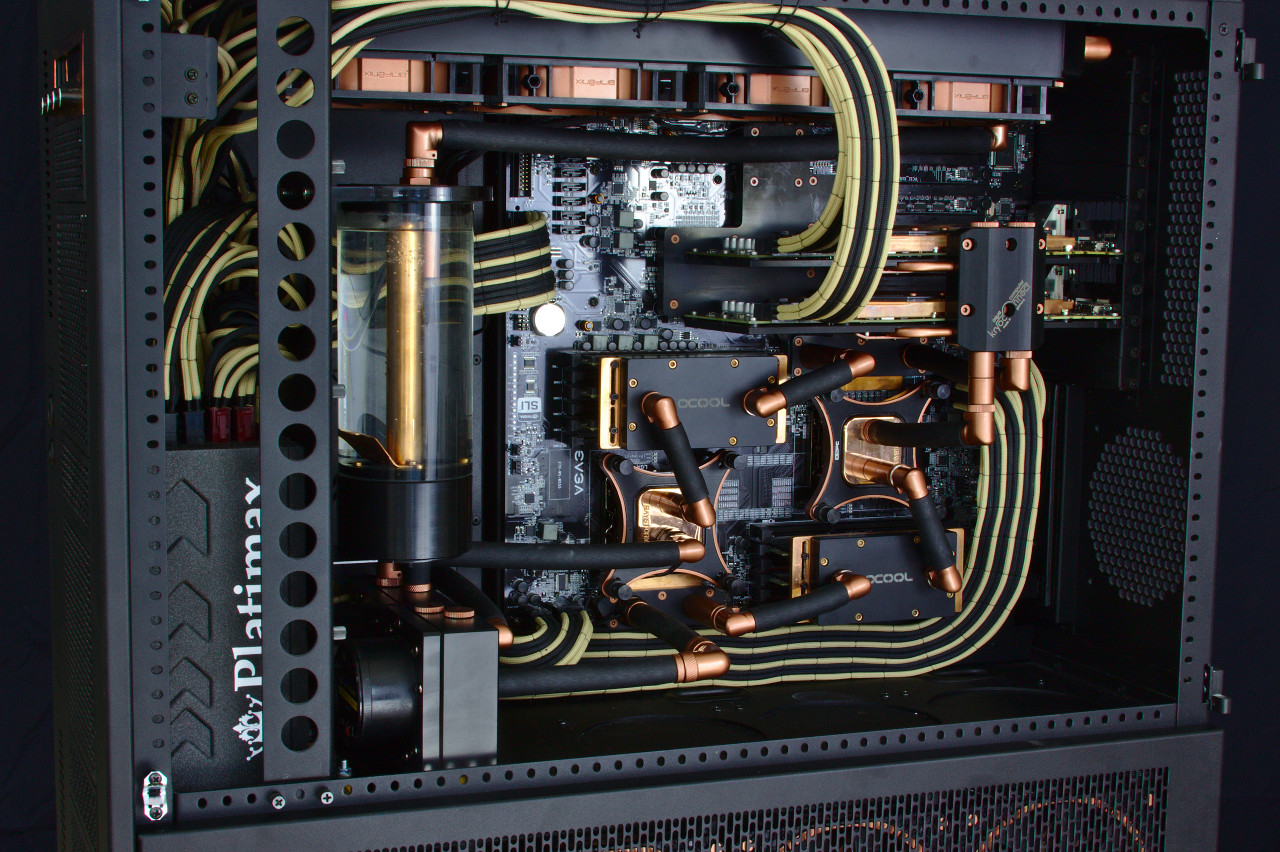
\includegraphics[width=120mm]{titlepic.jpg}

    \vfill

    \today\\
    Version 1.0.0
\end{titlingpage}
\frontmatter
\tableofcontents*

\mainmatter
\chapter{Text}
\lipsum[1]

\sffamily\lipsum[2]

\bfseries\lipsum[3]

\mdseries\ttfamily\lipsum[4]

\bfseries\ttfamily\lipsum[5]

\normalfont\scshape\lipsum[6]

\slshape\lipsum[7]

\scshape\lipsum[8]

\scslshape\lipsum[9]

\normalfont

\chapter{Tables}
\begin{table}
    \centering
    \caption{tabular inside float}
    \label{tab:float}
    \begin{tabular}{lll}
        \toprule
        \scshape Header 1 & \scshape Header 2 & \scshape Header 3 \\
        \midrule
        Content           & Content           & Content           \\
        Content           & Content           & Content           \\
        Content           & Content           & Content           \\
        Content           & Content           & Content           \\
        \bottomrule
    \end{tabular}
\end{table}

\lipsum[3]

\begin{center}
    \tabcaption{Tabular outside of float}
    \label{tab:outside}
    \begin{tabular}{lll}
        \toprule
        \scshape Header 1 & \scshape Header 2 & \scshape Header 3 \\
        \midrule
        Content           & Content           & Content           \\
        Content           & Content           & Content           \\
        Content           & Content           & Content           \\
        Content           & Content           & Content           \\
        \bottomrule
    \end{tabular}
\end{center}

\chapter{References and Hyperlinks}
This sentence refers to Table~\ref{tab:outside}.

This is a citation \cite{testitem}.

\href{https://hyperlink.com}{This is a hyperlink hiding behind text.}

\href{https://hyperlink.com}{\nolinkurl{https://hyperlink.com}}

\chapter{Sectional Headings}

This section illustrates the  style of \verb|\section|, \verb|\subsection| and
\verb|\subsubsection|.

\section{A Section}
\lipsum[2]

\subsection{A Subsection}
\lipsum[1]

\subsubsection{A subsubsection}
\lipsum[2]

\chapter{Code Listings}
\tikzset{external/export next=false}%
\begin{tcblisting}{%
        title=This Is a Code Listing,
        minted language=tex,
        listing side text,
        }
    \begin{tabular}{ll}
        a & a \\
        a & a \\
    \end{tabular}
\end{tcblisting}

\tikzset{external/export next=false}%
\begin{tcolorbox}[title=test]
    \lipsum[2]
\end{tcolorbox}

\tikzset{external/export next=false}%
\begin{tcolorbox}
    \lipsum[2]
\end{tcolorbox}

\chapter{Mathematics}

A numbered equation:
\begin{equation}
    y(x) = x^2 + 2x + 5
\end{equation}

An unnumbered equation:
\begin{equation*}
    x_{01,02} = -1 \pm 2j
\end{equation*}

An \verb|align| with some numbered and unnumbered lines:

\begin{align}
    \frac{\Phi}{i}
    & =
    \int_{0}^{\infty} \frac{dx}{x} \int_{0}^{l+m}
    \left[
        \frac{y dy}{\sqrt{x^2+y^2}} - \frac{(y-l) dy}{\sqrt{x^2+(y-l)^2}}
    \right]
    \nonumber
    \\
    &=
    \int_{0}^{\infty}
    \left[
        \sqrt{x^2 + (l+m)^2)} - \sqrt{x^2+l^2} - \sqrt{x^2+m^2}+x
    \right]
    \frac{dx}{x}
    \nonumber
    \\
    &= 
    \Bigg[
        \sqrt{x^2 + (l+m)^2} - \sqrt{x^2+l^2} - \sqrt{x^2+m^2}
        \nonumber
        \\
        & ~~~~~~~~~   + x - l \cdot \log{\frac{l+m+\sqrt{x^2+(l+m)^2}}{l+\sqrt{x^2+l^2}}}
        \nonumber
        \\
        & ~~~~~~~~~   - m \cdot \log{\frac{l+m+\sqrt{x^2+(l+m)^2}}{m+\sqrt{x^2+l^2}}} ~
    \Bigg]_0^{\infty}
    \label{eq:mISL:2}
    \\
    & \approx
    \left[ l \cdot \log{\frac{l+m}{l}} + m \cdot \log{\frac{l+m}{m}} \right]
    \label{eq:mISL:3}
\end{align}


\cleardoublepage
\begin{titlingpage*}
    \fullhexpage{da2}{ct4}
    \begin{vplace}
        \flushright\Huge\bfseries\sffamily\appendixpagename
    \end{vplace}
\end{titlingpage*}
\appendix
\chapterstyle{alpenappendix}
\chapter{An Appendix Chapter}
\lipsum[1-3]

\chapter{Another Appendix Chapter}
\lipsum[4-6]

\backmatter
\chapter{A Backmatter Chapter}
\lipsum[7-9]

\begin{thebibliography}{1}
    \bibitem{testitem}
        An Author, ``A Title``, 1979.
\end{thebibliography}
%% ============================================================== END CONTENT %
\end{document}
%</example>
% \fi
%^^A >>>
%
%^^A ------------------------------------------------------------------------- %
%^^A                                                  MULTI-LANGUAGE SUPPORT <<<
% \iffalse
%<*de>
\expandafter\newif\csname ifenglish\endcsname
\englishfalse
% \iffalse meta-comment
% -------------------------------------------------------- %
% Copyright (c) 2017 Raphael Frey rmfrey@runbox.com        %
% -------------------------------------------------------- %
%                                                          %
% This file  may be distributed and/or  modified under the %
% conditions of  the LaTeX Project Public  License, either %
% version 1.3c  of this  license or  (at your  option) any %
% later version. The latest version of this license is in: %
%                                                          %
%     http://www.latex-project.org/lppl.txt                %
%                                                          %
% and version 1.3c  or later is part  of all distributions %
% of LaTeX version 2008/05/04 or later.                    %
% -------------------------------------------------------- %
% \fi
%
%\CheckSum{0}
%
%
%^^A ------------------------------------------------------------------------- %
%^^A                                              DRIVER, PROVIDESCLASS ETC. <<<
% \iffalse
%<*driver>
\ProvidesFile{alpenthesis.dtx}
%</driver>
%<class>\NeedsTeXFormat{LaTeX2e}
%<class>\ProvidesClass{alpenthesis}%
%<*class>
    [2017/04/06 v0.0.1 PDF-LaTeX class for my thesis]
%</class>
%<*driver>
\expandafter\ifx\csname ifenglish\endcsname\relax
    \expandafter\newif\csname ifenglish\endcsname
    \englishtrue
\fi
\documentclass[a4paper,11pt,oneside]{ltxdoc}
\EnableCrossrefs
\CodelineIndex
\RecordChanges
% ----------------------------------------------- PACKAGES %
\usepackage[T1]{fontenc}
\usepackage[utf8]{inputenc}
\ifenglish
    \usepackage[english]{babel}
\else
    \usepackage[ngerman]{babel}
\fi
\usepackage{xcolor-solarized}
\usepackage[light,nott]{kpfonts}
\usepackage[scaled=0.8125]{DejaVuSansMono}
\usepackage{hypdoc}
\usepackage{tikz}
\usepackage{alpencolors}
\usepackage{booktabs}
\usepackage{imakeidx}
% ------------------------------------------ HELPER MACROS %
\newcommand*\pacname[1]{\textsf{#1}}
\newcommand*\code[1]{\texttt{#1}}
\newcommand*\athes{\pacname{alpenthesis}}
\newcommand*\memoir{\pacname{memoir}}
\begin{document} % ****************************** DOCUMENT %
    \DocInput{alpenthesis.dtx}
\end{document}
%</driver>
% \fi
%^^A >>>
%
%^^A ------------------------------------------------------------------------- %
%^^A                                                 GetFileInto, DoNotIndex <<<
% \GetFileInfo{alpenthesis.dtx}
% \DoNotIndex{\addtolength,\bfseries,\captiondelim,\captionnamefont}
% \DoNotIndex{\captiontitlefont,\checkandfixthelayout,\color,\Large}
% \DoNotIndex{\large,\LoadWithClassOptions,\maxsecnumdepth,\maxtocdepth}
% \DoNotIndex{\newcommand,\newfixedcaption,\pagestyle,\paperheight}
% \DoNotIndex{\paperwidth,\renewcommand,\RequirePackage,\setlength}
% \DoNotIndex{\setlrmarginsandblock,\setsecheadstyle,\setsubsecheadstyle}
% \DoNotIndex{\setsubsubsecheadstyle,\settrimmedsize,\settrims}
% \DoNotIndex{\setulmarginsandblock,\sffamily,\small,\stockaiii}
% \DoNotIndex{\stockwidth,\textsf,\texttt,\trimedge,\trimmarkscolor}
% \DoNotIndex{\trimtop}
% \DoNotIndex{\@chapapp,\addtodef,\afterchapskip,\afterchapternum}
% \DoNotIndex{\athes,\beforechapskip,\begin,\end}
% \DoNotIndex{\AT@bottomscreen,\chapnamefont,\chapnumfont}
% \DoNotIndex{\chapterheadstart,\chapternamenum,\chaptitlefont}
% \DoNotIndex{\edgewidth,\fadingIndex,\fi,\fill,\flushright,\foreach}
% \DoNotIndex{\globalcolorstrue,\height,\hspace,\HUGE,\includepdf}
% \DoNotIndex{\input,\iterstop,\iterstopvert,\j,\k,\LARGE,\leftTransp}
% \DoNotIndex{\MakeTextUppercase,\m,\makebox,\marginparsep,\marginparwidth}
% \DoNotIndex{\maxElementNumber,\midchapskip,\n,\newif,\newlength,\nobreak}
% \DoNotIndex{\numberOfHorizSides,\numberOfHorizElements,\offsetVert}
% \DoNotIndex{\par,\pgfkeysgetvalue,\pgfmathcos,\pgfmathmod,\pgfmathresult}
% \DoNotIndex{\pgfmathsetmacro,\pgfmathtruncatemacro,\pgfplotsset}
% \DoNotIndex{\printchaptername,\printchapternonum,\printchapternum}
% \DoNotIndex{\printchaptertitle,\x,\y,\resizebox}
% \DoNotIndex{\rightTransp,\rowtestcolor,\rule,\side,\spinemargin}
% \DoNotIndex{\textwidth,\thechapter,\thepage,\tikz,\tikzfading,\tikzset}
% \DoNotIndex{\usepackage,\usepgfplotslibrary,\usetikzlibrary,\vskip,\vspace}
%^^A>>>
%
%^^A ------------------------------------------------------------------------- %
%^^A                                                    TITLE, ABSTRACT, ToC <<<
% \author{Raphael Frey \\[1ex] \href{https://github.com/alpenwasser/}%
%                                     {\nolinkurl{https://github.com/alpenwasser/}}}
%
% \ifenglish
%   \title{The \athes\ Class\thanks{This document corresponds
%       to \athes~\fileversion, dated~\filedate.}}
%   \maketitle
%   \begin{abstract}
%        The \athes\  class is the  \LaTeX class I  wrote for my  thesis. It is
%        based on  the \memoir\  class and  is a  collection of  various custom
%        commands  and  configurations  to  suit my  personal  preferences  and
%        requirements. You may or  may not find some of it  useful, but keep in
%        mind that this is a class created  for a specific use case to cater to
%        a  select  few people's  preferences,  so  some  things may  not  seem
%        sensible or acceptable to you.
%
%        For  this  reason, the  class  does  not really  allow  for  a lot  of
%        customisation\footnotemark. It is primarily a ``fire-and-forget'' sort of affair.
%
%        \footnotetext{%
%            In principle,  most options and  commands from the  \memoir\ class
%            are present and  supported, but because this class loads  a lot of
%            packages  and preforms  a lot  of customization,  the results  may
%            sometimes  be undesired. I  have taken  no particular  precautions
%            when it comes to compatibility on  this level beyond what I needed
%            to make my personal configuration work as desired.}
%   \end{abstract}
% \else
%   \title{Die \athes-Klasse\thanks{Dieses Dokument entspricht
%          \athes~\fileversion, datiert~\filedate.}}
%   \maketitle
%   \begin{abstract}
%        Die \athes-Klasse  ist die \LaTeX-Klasse,  die ich f\"ur  meine Thesis
%        entwickelt habe,  aufbauend auf  der \memoir-Klasse. Sie  ist prim\"ar
%        eine Kollektion  von massgeschneiderten Befehlen  und Konfigurationen,
%        um   meine   pers\"onlichen   Bed\"urfnisse   und   Anforderungen   zu
%        erf\"ullen. Jemand  k\"onnte einen  Teil  davon allenfalls  n\"utzlich
%        finden. Man beachte  aber, dass diese Klasse  f\"ur einen spezifischen
%        Zweck f\"ur  einige wenige  Personen geschrieben  wurde. Somit m\"ogen
%        einige  Dinge  aus der  Sicht  der  geneigten Leserin  nicht  sinnvoll
%        implementiert sein.
%
%        Aus diesem  Grund ist  bei dieser  Klasse auch  nicht viel  Raum f\"ur
%        Konfiguration  vorgesehen\footnotemark. Es  ist  gr\"osstenteils  eine
%        ``fire-and-forget''-Angelegenheit.
%
%        \footnotetext{%
%            Im   Prinzip  werden   die  meisten   Optionen  und   Befehle  der
%            \pacname{memoir}-Klasse unterst\"utzt, aber  je nach Einstellungen
%            k\"onnten seltsame  Ergebnisse  auftreten,  da diese  Klasse viele
%            Packages l\"adt  und diverse Konfigurationen macht. Ich  habe hier
%            nicht explizit auf Kompatibilit\"at geachtet.}
%   \end{abstract}
% \fi
%
% \tableofcontents
%^^A >>>
%
%^^A ------------------------------------------------------------------------- %
%^^A                                                            INSTALLATION <<<
% \section{Installation}
% \label{sec:installation}
%
% \ifenglish
%    This section  deals with setting  up the \pacname{alpenthesis}  class and
%    setting up  a document with  it. Once you have generated  the \code{.cls}
%    class  file and  the \code{.pdf}  documentation (that  is: this  file, or
%    its  equivalent  in  another  language), or  have  received  those  files
%    from  somebody,  you  will   need  to  place  the  \code{alpenthesis.cls}
%    file  in  the  directory  of  your document  and  then  activate  it  via
%    |\documentclass{alpenthesis}|. See the \code{example.tex} for an example.
%
%    ^^A\inputminted[linenos=true,numbersep=4pt,fontsize=\footnotesize]{tex}{example.tex}
%   ^^A TODO: File structure tree with the needed files.
% \else
%    Dieser      Abschnitt      erkl\"art       die      Installation      der
%    \pacname{alpenthesis}-Klasse  und  erl\"autert,   wie  man  ein  Dokument
%    mit  ihr einrichtet. Nachdem  man  die \code{.cls}  Klassendatei und  die
%    Dokumentation  (dieses  Dokument,   oder  ein  anderssprachiges  Pendant)
%    generiert oder diese Dateien von  einer anderen Quelle erhalten hat, muss
%    man die Klassendatei \code{alpenthesis.cls} im selben Verzeichnis wie das
%    zu generierende Dokument platzieren und via |\documentclass{alpenthesis}|
%    aktivieren. Siehe  die  Datei   \code{example.tex},  welche  mitgeliefert
%    worden sein sollte.
% \fi
%^^A >>>
%
%^^A ------------------------------------------------------------------------- %
%^^A                                                          USER INTERFACE <<<
% \ifenglish
%    \section{User Interface}
%    \label{sec:user-interface}
% \else
%    \section{Benutzer-Interface}
%    \label{sec:user-interface}
% \fi
%
% |\documentclass\oarg{args}{alpenthesis}|\vspace{1em}
%
% \ifenglish
%    Loads  the  \athes\  class  with options  \meta{args}. Those  options  are
%    directly passed through to the  underlying \memoir\ class, so most options
%    for \memoir\  can be  specified. However, some may  be less  sensible than
%    others, given all the other configurations \athes\ makes.
%
%    If you require heavy customisation,  it is probably recommendable to start
%    off with the \memoir\ class itself as a base and build from there, relying
%    on its excellent documentation.
% \else
%    L\"adt    die    \athes-Klasse    mit    den    spezifizierten    Optionen
%    \meta{args}. Diese   Optionen   werden   direkt   an   die   unterliegende
%    \memoir-Klasse  weitergegeben. Somit  k\"onnen   beinahe  alle  f\"ur  die
%    \memoir-Klasse verf\"ugbaren Optionen  geladen werden. Man beachte jedoch,
%    dass  nicht unbedingt  alle  Optionen Sinn  machen,  da die  \athes-Klasse
%    selbst noch einige Konfigurationen vornimmt.
%
%    M\"ochte man  starke Individualisierungen  vornehmen, macht  es vermutlich
%    mehr Sinn, die  \memoir-Klasse direkt zu laden und  anhand der exzellenten
%    Dokumentation die gew\"unschte Konfiguration zu erstellen.
% \fi
% \DescribeMacro{\aiiistock}
% \DescribeMacro{\showtrimson}
% \DescribeMacro{\showtrimsoff}
% \ifenglish
%    Sets the  stock size to  A3 paper, keeping the  trimmed paper size  at A4,
%    vertically and  horizontally centered. Prints trim  marks for the  A4 page
%    centered on the A3 sheet.
%
%    To disable  trim marks,  you can  use the  |\showtrimsoff|. |\showtrimson|
%    will  enable them  again. Refer  to the  \memoir\  documentation for  more
%    information.
% \else
%    Setzt  die  Bogengr\"osse  auf  A3,  w\"ahrend  die  bedruckte  Seite  auf
%    A4  behalten wird.   Der  bedruckte Bereich  ist  vertikal und  horizontal
%    zentriert auf dem A3-Bogen. Druckt Markierungen um die A4-Seite.
%
%    Um  die  Markierungen zu  entfernen  kann  der |\showtrimsoff|-Befehl  von
%    \memoir\ benutzt werden. |\showtrimson| schaltet sie wieder ein. Siehe die
%    \memoir-Dokumentation.
% \fi
%
% \DescribeMacro{\hextrue}
% \DescribeMacro{\hexfalse}
% \ifenglish
%    In order to save time when compiling a document, the |\hexfalse| value can
%    be set in the preamble. This leads to the hexagon grind being omitted from
%    the chapter style.
%
%    Setting |\hextrue|  will enable the hexagons. This  lengthens compile time
%    significantly.
%
%    The principle is similar to the  |draft| option which is available in many
%    document classes and  packages. Personally I do not tend to  use that much
%    though because of  all the usual things which come  with |draft|, which is
%    why I decided to implement a separate command.
% \else
%    Um  Zeit  zu  sparen  beim   Kompilieren,  kann  man  |\hexfalse|  in  der
%    Pre\"aambel setzen. Dies f\"uhrt dazu,  dass die Hexagons im Kapitel-Style
%    nicht gedruckt werden.
%
%    Den  Wert   |\hextrue|  zu  setzen, aktiviert die  Hexagons. Dies
%    verl\"angert die Kompilierzeit bedeutend.
%
%    Das  Prinzip  ist  \"ahnlich  wie  die  in  vielen  Packages  und  Klassen
%    verf\"ugbare |draft|-Option. Da  ich diese  jedoch f\"ur  meinen Geschmack
%    im  Normalfall  etwas  viele  unerw\"unschte Seiteneffekte  hat,  ist  ein
%    unabh\"angiger Switch implementiert.
% \fi
%^^A >>>
%
% \StopEventually{\PrintIndex}
%^^A ------------------------------------------------------------------------- %
%^^A                                                          IMPLEMENTATION <<<
% \section{Implementation}
% \label{sec:implementation}
%
%^^A ---------------------------------------------- Loading the memoir Class <<<
% \ifenglish
%    \subsection{Loading the Base Class (\memoir)}
%    \label{subsec:memload}
%    The underlyng  class is  \memoir, and  all options  passed to  the \athes\
%    class are directly  passed on to \memoir\  via the |\LoadClassWithOptions|
%    command.
%
%    Additionally, the two hexagon configuration switches are defined.
% \else
%    \subsection{Laden der Basisklasse (\memoir)}
%    \label{subsec:memload}
%    Die  zugrundeliegende Klasse  ist \memoir. Alle  an \athes\  \"ubergebenen
%    Optionen   werden   direkt   an   die   \memoir-Klasse   \"ubergeben   via
%    |\LoadClassWithOptions|.
%
%    Im Weiteren werden  die beiden Konfigurations-Booloeans f\"ur die Hexagons
%    hier definiert.
% \fi
% \color{sqB}
%^^A Need the class guards to prevent the macro code from being included again
%^^A in example.tex and the German .tex file
% \iffalse
%<*class>
% \fi
%    \begin{macrocode}
\LoadClassWithOptions{memoir}
\newif\ifhex
\newif\ifpaper
%    \end{macrocode}
% \iffalse
%</class>
% \fi
% \color{black}
%^^A>>>
%^^A ---------------------------------------------- Fonts, inputenc, fontenc <<<
% \ifenglish
%    \subsection{General Configuration}
%    \label{subsec:general-config}
%    We choose  the \pacname{kpfonts}  Package for serif  and sans  serif fonts
%    with the  |light| option,  and \pacname{DejaVuSansMono} as  our typewriter
%    font. Also, we  ensure that we  can write our  source code files with UTF8
%    characters and have T1 font encoding for our output.
% \else
%    \subsection{Allgemeine Konfiguration}
%    \label{subsec:general-config}
%    Wir  w\"ahlen  \pacname{kpfonts} als  unsere  Schriftart  f\"ur Serif  und
%    Sans-Serif,  mit  der  |light|-Option,  und  \pacname{DejaVuSansMono}  als
%    unsere  Monospace-Schriftart. Wir  stellen   ebenfalls  sicher,  dass  wir
%    UTF8-Input in unserem  Quelltext haben k\"onnen und dass der  Output in T1
%    codiert wird.
% \fi
% \color{sqB}
% \iffalse
%<*class>
% \fi
%    \begin{macrocode}
\RequirePackage[rmx,nott,intlimits,sumlimits]{kpfonts}
\RequirePackage[scaled=0.8125]{DejaVuSansMono}
\RequirePackage[utf8]{inputenc}
\RequirePackage[T1]{fontenc}
%    \end{macrocode}
% \iffalse
%</class>
% \fi
% \color{black}
%^^A>>>
%^^A ------------------------------------------------ DOCUMENT COLOR PALETTE <<<
% \ifenglish
%    \subsection{Document Color Palette}
%    \label{subsec:colors}
%    We  define the  following  colors  as our  document  colors  in a  central
%    location.  This allows easy modification  of document colors while keeping
%    the entire document consistent.
% \else
%    \subsection{Farbpalette des Dokuments}
%    \label{subsec:colors}
%    Wir  definieren  die  folgenden  Farben  f\"ur  unser  Dokument  an  einer
%    zentralen Stelle.  Dies erlaubt es,  die Farbpalette des Dokuments einfach
%    zu  modifizieren  und  dabei  die   Farben  \"uber  das  gesamte  Dokument
%    konsistent zu behalten.
% \fi
% \color{sqB}
% \iffalse
%<*class|colors>
%^^A We  extract the  color information into  a package for  use in  the class
%^^A documentation.
%<colors>\ProvidesPackage{alpencolors}[2017/04/08 v1.0 color palette for alpenthesis]
% \fi
%    \begin{macrocode}
\RequirePackage{xcolor}
\globalcolorstrue
\newcommand*\testcolor[1]{\tikz \fill[#1] (0em,0ex) rectangle (2em,2ex);}
\newcommand*\rowtestcolor[1]{#1 & \tikz \fill[#1] (0em,0ex) rectangle (2em,2ex);}
%    \end{macrocode}
% \iffalse
%</class|colors>
% \fi
% \color{black}
% \ifenglish
%    \subsubsection{Dark-ish Colors}
%    \label{subsubsec:darkish}
% \else
%    \subsubsection{Eher Dunkle Farben}
%    \label{subsubsec:darkish}
% \fi
% \begin{center}
%     \small
%     \begin{tabular}{lllllllllll}
%         \toprule
%         \rowtestcolor{da0} &
%         \rowtestcolor{da1} &
%         \rowtestcolor{da2} &
%         \rowtestcolor{da3} &
%         \rowtestcolor{da4} \\
%         \bottomrule
%     \end{tabular}
% \end{center}
% \color{sqB}
% \iffalse
%<*class|colors>
% \fi
%    \begin{macrocode}
\definecolor{da0}{HTML}{002B36}  \definecolor{da1}{HTML}{073642}
\definecolor{da2}{HTML}{008080}  \definecolor{da3}{HTML}{800080}
\definecolor{da4}{HTML}{404040}
%    \end{macrocode}
% \iffalse
%</class|colors>
% \fi
% \color{black}
% \ifenglish
%    \subsubsection{Bright-ish Colors}
%    \label{subsubsec:brightish}
% \else
%    \subsubsection{Eher helle Farben}
%    \label{subsubsec:brightish}
% \fi
% \begin{center}
%     \small
%     \begin{tabular}{lllllllllll}
%         \toprule
%         \rowtestcolor{br0} &
%         \rowtestcolor{br1} &
%         \rowtestcolor{br2} \\
%         \bottomrule
%     \end{tabular}
% \end{center}
% \color{sqB}
% \iffalse
%<*class|colors>
% \fi
%    \begin{macrocode}
\definecolor{br0}{HTML}{BEB9AA}  \definecolor{br1}{HTML}{EEE8D5}
\definecolor{br2}{HTML}{FDF6E3}
%    \end{macrocode}
% \iffalse
%</class|colors>
% \fi
% \color{black}
% \ifenglish
%    \subsubsection{Contrast Color Palette}
%    \label{subsubsec:contrast}
% \else
%    \subsubsection{Kontrastfarben}
%    \label{subsubsec:contrast}
% \fi
% \begin{center}
%     \small
%     \begin{tabular}{lllllllllll}
%         \toprule
%         \rowtestcolor{ct0} &
%         \rowtestcolor{ct1} &
%         \rowtestcolor{ct2} &
%         \rowtestcolor{ct3} &
%         \rowtestcolor{ct4} \\
%         \rowtestcolor{ct5} &
%         \rowtestcolor{ct6} \\
%         \bottomrule
%     \end{tabular}
% \end{center}
% \color{sqB}
% \iffalse
%<*class|colors>
% \fi
%    \begin{macrocode}
\definecolor{ct0}{HTML}{CB4B16}  \definecolor{ct1}{HTML}{DC322F}
\definecolor{ct2}{HTML}{DC3682}  \definecolor{ct3}{HTML}{268BD2}
\definecolor{ct4}{HTML}{2AA198}  \definecolor{ct5}{HTML}{B58900}
\definecolor{ct6}{HTML}{859900}  \definecolor{sq0}{HTML}{F7FBFF}
%    \end{macrocode}
% \iffalse
%</class|colors>
% \fi
% \color{black}
% \ifenglish
%    \subsubsection{Sequential Color Palette}
%    \label{subsubsec:sequential}
% \else
%    \subsubsection{Sequentielle Farb-Palette}
%    \label{subsubsec:sequential}
% \fi
% \begin{center}
%     \small
%     \begin{tabular}{lllllllllll}
%         \toprule
%         \rowtestcolor{sq0} &
%         \rowtestcolor{sq1} &
%         \rowtestcolor{sq2} &
%         \rowtestcolor{sq3} &
%         \rowtestcolor{sq4} \\
%
%         \rowtestcolor{sq5} &
%         \rowtestcolor{sq6} &
%         \rowtestcolor{sq7} &
%         \rowtestcolor{sq8} &
%         \rowtestcolor{sq9} \\
%
%         \rowtestcolor{sqA} &
%         \rowtestcolor{sqB} &
%         \rowtestcolor{sqC} \\
%         \bottomrule
%     \end{tabular}
% \end{center}
% \color{sqB}
% \iffalse
%<*class|colors>
% \fi
%    \begin{macrocode}
\definecolor{sq1}{HTML}{EFF3FF}  \definecolor{sq2}{HTML}{DECDF7}
\definecolor{sq3}{HTML}{C6DBEF}  \definecolor{sq4}{HTML}{BDD7E7}
\definecolor{sq5}{HTML}{9ECAE1}  \definecolor{sq6}{HTML}{6BAED6}
\definecolor{sq7}{HTML}{4292C6}  \definecolor{sq8}{HTML}{3182BD}
\definecolor{sq9}{HTML}{2171B5}  \definecolor{sqA}{HTML}{08519C}
\definecolor{sqB}{HTML}{084594}  \definecolor{sqC}{HTML}{08306B}
%    \end{macrocode}
% \iffalse
%</class|colors>
% \fi
% \color{black}
% \ifenglish
%    \subsubsection{Divergent color palette}
%    \label{subsubsec:divergent}
% \else
%    \subsubsection{Divergierende Farb-Palette}
%    \label{subsubsec:divergent}
% \fi
% \begin{center}
%     \small
%     \begin{tabular}{lllllllllll}
%         \toprule
%         \rowtestcolor{dv-7} &
%         \rowtestcolor{dv-6} &
%         \rowtestcolor{dv-5} &
%         \rowtestcolor{dv-4} &
%         \rowtestcolor{dv-3} \\
%
%         \rowtestcolor{dv-2} &
%         \rowtestcolor{dv-1} &
%         \rowtestcolor{dv+0} &
%         \rowtestcolor{dv+1} &
%         \rowtestcolor{dv+2} \\
%
%         \rowtestcolor{dv+3} &
%         \rowtestcolor{dv+4} &
%         \rowtestcolor{dv+5} &
%         \rowtestcolor{dv+6} &
%         \rowtestcolor{dv+7} \\
%         \bottomrule
%     \end{tabular}
% \end{center}
% \color{sqB}
% \iffalse
%<*class|colors>
% \fi
%    \begin{macrocode}
\definecolor{dv-7}{HTML}{8E0152} \definecolor{dv-6}{HTML}{C51B7D}
\definecolor{dv-5}{HTML}{D01C8B} \definecolor{dv-4}{HTML}{DE77AE}
\definecolor{dv-3}{HTML}{E9A3C9} \definecolor{dv-2}{HTML}{F1B6DA}
\definecolor{dv-1}{HTML}{FDE0EF} \definecolor{dv+0}{HTML}{F7F7F7}
\definecolor{dv+1}{HTML}{D1E5F0} \definecolor{dv+2}{HTML}{92C5DE}
\definecolor{dv+3}{HTML}{67A9CF} \definecolor{dv+4}{HTML}{4393C3}
\definecolor{dv+5}{HTML}{0571B0} \definecolor{dv+6}{HTML}{2166AC}
\definecolor{dv+7}{HTML}{053061}
%    \end{macrocode}
% \iffalse
%</class|colors>
% \fi
% \color{black}
% \ifenglish
%    \subsubsection{Qualitative Color Palette}
%    \label{subsubsec:qualitative}
% \else
%    \subsubsection{Qualitative Farb-Palette}
%    \label{subsubsec:qualitative}
% \fi
% \begin{center}
%     \small
%     \begin{tabular}{lllllllllll}
%         \toprule
%         \rowtestcolor{q0} &
%         \rowtestcolor{q1} &
%         \rowtestcolor{q2} &
%         \rowtestcolor{q3} &
%         \rowtestcolor{q4} \\
%
%         \rowtestcolor{q5} &
%         \rowtestcolor{q6} &
%         \rowtestcolor{q7} \\
%         \bottomrule
%     \end{tabular}
% \end{center}
% \color{sqB}
% \iffalse
%<*class|colors>
% \fi
%    \begin{macrocode}
\definecolor{q0}{named}{ct3}   \definecolor{q1}{named}{sqB}
\definecolor{q2}{named}{ct2}   \definecolor{q3}{named}{da3}
\definecolor{q4}{HTML}{FEC44F} \definecolor{q5}{named}{ct0}
\definecolor{q6}{HTML}{80EA82} \definecolor{q7}{HTML}{2E7D32}
%    \end{macrocode}
% \iffalse
%</class|colors>
% \fi
% \color{black}
%^^A NOTE: each \rowtestcolor command requires two columns!
%^^A >>>
%^^A --------------------------------------------------- TikZ, PGF, PGFPLOTS <<<
% \ifenglish
%    \subsection{Ti\emph{k}Z, \textsc{pgfplots}}
%    \label{subsec:tikz-pgfplots}
% \else
%    \subsection{Ti\emph{k}Z, \textsc{pgfplots}}
%    \label{subsec:tikz-pgfplots}
% \fi
% \color{sqB}
% \iffalse
%<*class>
% \fi
%    \begin{macrocode}
\RequirePackage{tikz}
\usetikzlibrary{calc}
\usetikzlibrary{fadings}
\RequirePackage{pgfplots}
\pgfplotsset{compat=1.14}
\usepgfplotslibrary{external}
\tikzexternalize[prefix=cache/,optimize command away=\includepdf]
%    \end{macrocode}
% \iffalse
%</class>
% \fi
% \color{black}
%^^A >>>
%^^A -------------------------------------------------- HEXAGON CALCULATIONS <<<
% \ifenglish
%    \subsection{Hexagon Calculations}
%    \label{subsec:hexagon-calcs}
%    In this section,  the various required calculations for  the hexagon grids
%    are made. The basis is the number  of hexagons sides (not hexagons!) which
%    are to fit into one page width. Going  from there, the height of a hexagon
%    as well as the number of rows and columns are calculated.
% \else
%    \subsection{Berechnungen f\"ur Hexagons}
%    \label{subsec:hexagon-calcs}
%    An  dieser   Stelle  werden   diverse  Berechnungen  f\"ur   die  Hexagons
%    ausgef\"uhrt.  Grundlage ist die  Anzahl Hexagon-Seitenl\"angen (nicht die
%    Anzahl  Hexagons!), welche  in eine  Seitenbreite passt. Darauf  basierend
%    werden die halbe H\"ohe eines Hexagons sowie die Anzahl Spalten und Zeilen
%    berechnet.
% \fi
% \color{sqB}
% \iffalse
%<*class>
% \fi
%    \begin{macrocode}
\pgfmathsetmacro\AT@paperwidth{21}
\pgfmathsetmacro\AT@paperheight{29.7}
\pgfmathsetmacro\AT@numberOfSidesHorizontally{22}
\pgfmathsetmacro\AT@side
    {\AT@paperwidth / \AT@numberOfSidesHorizontally}
\pgfmathtruncatemacro\AT@totCols
    {0.666667 * \AT@numberOfSidesHorizontally + 1}
\pgfmathcos{30}
\pgfmathsetmacro\AT@height
    {\pgfmathresult * \AT@side}
\pgfmathtruncatemacro\AT@numberOfHeightsVertically
    {\AT@paperheight / \AT@height}
\pgfmathtruncatemacro\AT@totRows
    {0.5 * \AT@numberOfHeightsVertically + 1}
\pgfmathtruncatemacro\AT@totRowsChap
    {0.1333 * \AT@numberOfHeightsVertically + 1}
%    \end{macrocode}
% \iffalse
%</class>
% \fi
% \color{black}
% \ifenglish
%    If the print version is to be generated, a uniform color for each hexagon,
%    depending on its horizontal and vertical position, is calculated:
% \else
%    Falls  die Druckversion  erstellt werden  soll, wird  eine uniforme  Farbe
%    f\"ur  jedes Hexagon,  abh\"angig von  seiner horizontalen  und vertikalen
%    Position, generiert:
% \fi
% \color{sqB}
% \iffalse
%<*class>
% \fi
%    \begin{macrocode}
\AtBeginDocument{%
    \ifpaper
        \foreach \y in {0,...,\AT@totRowsChap} {%
            \foreach \x in {0,...,\AT@totCols}{%
                \pgfmathsetmacro\mix
                    {100 * \x / \AT@totCols}%
                \pgfmathsetmacro\mixvert
                    {100 * \y / \AT@totRowsChap}%
                \colorlet{hex-\x}{white!\mix!br0}%
                \colorlet{hex-\x-\y}{white!\mixvert!hex-\x}%
                \colorlet{hexframecol-\x}{white!\mix!br2}%
                \colorlet{hexframecol-\x-\y}
                    {white!\mixvert!hexframecol-\x}%
                \colorlet{chapcol-\x}{dv-4!\mix!dv-7}%
                \colorlet{chapcol-\x-\y}
                    {dv-2!\mixvert!chapcol-\x}%
                \colorlet{appcol-\x}{ct4!\mix!da2}%
                \colorlet{appcol-\x-\y}{white!\mixvert!appcol-\x}%
            }%
        }%
%    \end{macrocode}
% \iffalse
%</class>
% \fi
% \color{black}
% \ifenglish
%    For the  electronic version,  fadings are used  instead. Unfortunately, we
%    cannot simply have one global fading  which applies to all hexagons (since
%    each hexagon is  a single path)\footnotemark, so one  fading is calculated
%    for each  hexagon based  on its  horizontal position. The  vertical fading
%    effect is later achieved by  overlaying a white-to-transparent screen from
%    the grid's bottom edge. Maybe one day I'll figure out how to combine these
%    into one single and nice step.
%
%    \footnotetext{%
%        Or more accurately: I  have not been able to find  a way to accomplish
%        this.}
% \else
%    F\"ur die elektronische Version werden stattdessen Fadings benutzt. Leider
%    kann  nicht  einfach   ein  globales  Fading  definiert   und  \"uber  das
%    gesamte  Gitter  gelegt  werden  (da   jedes  einzelne  Hexagon  ein  Pfad
%    ist)\footnotemark, deshalb  wird f\"ur jedes Hexagon  ein Fading bestimmt,
%    abh\"angig  von   der  horizontalen  Position  im   Gitter. Der  vertikale
%    Fading-Effekt  wird  mit   einem  weiss-zu-transparenten  Fading  erzeugt,
%    welches dem gesamten Gitter  von unten \"uberlagert wird. Vielleicht finde
%    ich  eines  Tages eine  clevere  Variante,  die  beiden Effekte  in  einen
%    einzelnen, eleganten Schritt zu kombinieren.
%
%    \footnotetext{%
%        Oder genauer  gesagt: Ich habe  bisher nicht herausgefunden,  wie dies
%        m\"oglich w\"are.}
% \fi
% \color{sqB}
% \iffalse
%<*class>
% \fi
%    \begin{macrocode}
    \else
        \foreach \x in {0,...,\AT@totCols}{%
            \pgfmathsetmacro\leftTransp
                {100 *  \x    / \AT@totCols}%
            \pgfmathsetmacro\rightTransp
                {100 * (\x+1) / \AT@totCols}%
            \tikzfading[%
                name=hexfade \x,
                right color=transparent!\rightTransp,
                left color=transparent!\leftTransp]%
        }%
    \fi
}
\newcommand\AT@providehexagonpath[3]{%
    ($(current page.north west) +
        (1.5 * #1 * \AT@side,
            #3 * \AT@height - #2 * 2 * \AT@height)$)
    -- ++(   0:\AT@side)
    -- ++( -60:\AT@side)
    -- ++(-120:\AT@side)
    -- ++(-180:\AT@side)
    -- ++(-240:\AT@side) -- cycle;
}
%    \end{macrocode}
% \iffalse
%</class>
% \fi
% \color{black}
%^^A >>>
%^^A ------------------------------------------ HEXAGON FULL PAGE BACKGROUND <<<
% \ifenglish
%    \subsection{Hexagon Page Background}
%    \label{subsec:hexagon-background}
% \else
%    \subsection{Hexagon Seitenhintergrund}
%    \label{subsec:hexagon-background}
% \fi
% \color{sqB}
% \iffalse
%<*class>
% \fi
%    \begin{macrocode}
\newcommand\fullhexpage[2]{%
    \ifhex
        \tikzset{external/export next=false}%
        \begin{tikzpicture}[remember picture,overlay,x=1cm,y=1cm]
            \path[clip]
                (current page.north west)
                rectangle
                (current page.south east);
            \foreach \y in {0,...,\AT@totRows} {%
                \foreach \x in {0,...,\AT@totCols} {%
                    \pgfmathsetmacro\AT@isodd{mod(\x,2)}
                    \fill[fill=br2,draw=br1]
                        \AT@providehexagonpath{\x}{\y}{\AT@isodd}
                }
            }
            % Create vertical contrast bar on left side.
            % Put it inside scope for clipping.
            \begin{scope}
                \path[clip]
                    (current page.north west)
                    rectangle
                    ($(current page.south west) +
                        (3.5 * \AT@side,0)$);
                \foreach \y in {0,...,\AT@totRows} {%
                    \foreach \x in {0,...,2} {%
                        \pgfmathsetmacro\AT@isodd{mod(\x,2)}
                        \fill[fill=#1,draw=#2]
                            \AT@providehexagonpath{\x}{\y}{\AT@isodd}
                    }
                }
            \end{scope}
        \end{tikzpicture}%
    \fi
}
%    \end{macrocode}
% \iffalse
%</class>
% \fi
% \color{black}
%^^A>>>
%^^A ------------------------------------------------------------- tcolorbox <<<
% \ifenglish
%    \subsection{\pacname{tcolorbox}}
%    \label{subsec:tcolorbox}
%
%    Keeping with the theme of angled things, we define an octagon shape
%    as the surrounding shape for \pacname{tcolorbox}.
% \else
%    \subsection{\pacname{tcolorbox}}
%    \label{subsec:tcolorbox}
%
%    Um zum allgemeinen Thema der gewinkelten Dinge zu passen, wird ein Oktagon
%    als Form f\"ur den Rahmen der \pacname{tcolorbox}-Elemente definiert.
% \fi
% \color{sqB}
% \iffalse
%<*class>
% \fi
%    \begin{macrocode}
\RequirePackage{tcolorbox}
\tcbuselibrary{minted}
\tcbuselibrary{skins}
\tcbset{%
    colback=br2,
    coltitle=br2,
    colframe=da1,
    fonttitle=\sffamily,
    minted options={autogobble},
    enhanced,
    frame code={
        \draw[very thick]
               ([xshift=-3mm,yshift=+1mm]frame.north east)
            -- ([xshift=+0mm,yshift=-2mm]frame.north east)
            -- ([xshift=+0mm,yshift=+2mm]frame.south east)
            -- ([xshift=-3mm,yshift=-1mm]frame.south east)
            -- ([xshift=+3mm,yshift=-1mm]frame.south west)
            -- ([xshift=-0mm,yshift=+2mm]frame.south west)
            -- ([xshift=-0mm,yshift=-2mm]frame.north west)
            -- ([xshift=+3mm,yshift=+1mm]frame.north west)
            -- cycle;
    },
    interior titled code={%
        \path[tcb fill interior]
               ([xshift=-2.7mm,yshift=+1.3mm]interior.north east)
            -- ([xshift=+0.3mm,yshift=-1.7mm]interior.north east)
            -- ([xshift=+0.3mm,yshift=+1.7mm]interior.south east)
            -- ([xshift=-2.7mm,yshift=-1.3mm]interior.south east)
            -- ([xshift=+2.7mm,yshift=-1.3mm]interior.south west)
            -- ([xshift=-0.3mm,yshift=+1.7mm]interior.south west)
            -- ([xshift=-0.3mm,yshift=-1.7mm]interior.north west)
            -- ([xshift=+2.7mm,yshift=+1.3mm]interior.north west)
            -- cycle;
    },
    interior code={%
        \path[tcb fill interior]
               ([xshift=-2.7mm,yshift=+1.3mm]interior.north east)
            -- ([xshift=+0.3mm,yshift=-1.7mm]interior.north east)
            -- ([xshift=+0.3mm,yshift=+1.7mm]interior.south east)
            -- ([xshift=-2.7mm,yshift=-1.3mm]interior.south east)
            -- ([xshift=+2.7mm,yshift=-1.3mm]interior.south west)
            -- ([xshift=-0.3mm,yshift=+1.7mm]interior.south west)
            -- ([xshift=-0.3mm,yshift=-1.7mm]interior.north west)
            -- ([xshift=+2.7mm,yshift=+1.3mm]interior.north west)
            -- cycle;
    },
    title code={%
        \path[tcb fill frame]
               ([xshift=-3mm,yshift=+1mm]frame.north east)
            -- ([xshift=+0mm,yshift=-2mm]frame.north east)
            -- ([xshift=+0.3mm,yshift=-2mm]interior.north east)
            -- ([xshift=-3mm,yshift=+1mm]interior.north east)
            -- ([xshift=+3mm,yshift=+1mm]interior.north west)
            -- ([xshift=-0.3mm,yshift=-2mm]interior.north west)
            -- ([xshift=-0mm,yshift=-2mm]frame.north west)
            -- ([xshift=+3mm,yshift=+1mm]frame.north west)
            -- cycle;
    }
}
%    \end{macrocode}
% \iffalse
%</class>
% \fi
% \color{black}
%^^A >>>
%^^A ------------------------------------ OTHER PACKAGES WOTHOUT MUCH CONFIG <<<
% \ifenglish
%    \subsection{Other Packages}
%    \label{subsec:other-packages}
% \else
%    \subsection{Andere Packages}
%    \label{subsec:other-packages}
% \fi
% \color{sqB}
% \iffalse
%<*class>
% \fi
%    \begin{macrocode}
\RequirePackage[%
    pdfauthor=alpenwasser,
    pdfsubject={LaTeX document design},
    pdftitle={alpenwasser's thesis},
    bookmarksnumbered=true,
    pdfkeywords={LaTeX,design,alpenwasser,thesis,class,hexagons},
    colorlinks=true,
    linkcolor=sqB,
    citecolor=ct4,
    urlcolor=dv-6]{hyperref}
\RequirePackage[english]{babel}
\RequirePackage{amsmath}
\RequirePackage[separate-uncertainty=true]{siunitx}
\RequirePackage{counttexruns}
%    \end{macrocode}
% \iffalse
%</class>
% \fi
% \color{black}
%^^A >>>
%^^A --------------------------------------------------------- MEMOIR CONFIG <<<
%
%^^A -------------------------------------------------------- General Config <<<
% \ifenglish
%   \subsection{\memoir\ Configuration}
%   \label{subsec:memconfig}
%   \subsubsection{General Configuration}
%   \label{subsubsec:memoir:general-config}
% \else
%   \subsection{\memoir-Konfiguration}
%   \label{subsec:memconfig}
%   \subsubsection{Allgemeine Konfiguration}
%   \label{subsubsec:memoir:general-config}
% \fi
% \color{sqB}
% \iffalse
%<*class>
% \fi
%    \begin{macrocode}
\maxsecnumdepth{subsubsection}
\maxtocdepth{subsubsection}
\chapterstyle{veelo}
%    \end{macrocode}
% \iffalse
%</class>
% \fi
% \color{black}
%^^A>>>
%^^A ----------------------------------------------------------- Page Layout <<<
% \ifenglish
%     \subsubsection{Page Layout}
%     \label{subsubsec:page-layout}
% \else
%     \subsubsection{Seiten-Layout}
%     \label{subsubsec:page-layout}
% \fi
% \color{sqB}
% \iffalse
%<*class>
% \fi
%    \begin{macrocode}
\newcommand\aiiistock{%
    \stockaiii
    \settrimmedsize{297mm}{210mm}{*}
    \setlength{\trimtop}{\stockheight}
    \addtolength{\trimtop}{-\paperheight}
    \setlength{\trimedge}{\stockwidth}
    \addtolength{\trimedge}{-\paperwidth}
    \settrims{0.5\trimtop}{0.5\trimedge}
    \renewcommand*{\trimmarkscolor}{\color{red}}
    \showtrimson
    \checkandfixthelayout
}
\showtrimsoff
\setlrmarginsandblock{0.142857111\paperwidth}{0.190476190\paperwidth}{*}
\setulmarginsandblock{0.111111111\paperheight}{*}{1.5}%
\checkandfixthelayout
%    \end{macrocode}
% \iffalse
%</class>
% \fi
% \color{black}
%^^A>>>
%^^A -------------------------------------------- Sectional Title Formatting <<<
% \ifenglish
%    \subsubsection{Sectional Title Fonts and Styles} ^^A ---- Sec Title Fonts %
%    \label{subsubsec:title-fonts}
%    Sets font styles and other stylistic attributes for headings.
% \else
%    \subsubsection{Schriftarten und Stil f\"ur Titel von Abschnitten}
%    \label{subsubsec:title-fonts}
%    Definiert Schriftarten und andere Stil-Attribute f\"ur \"Uberschriften.
% \fi
% \color{sqB}
% \iffalse
%<*class>
% \fi
%    \begin{macrocode}
\setsecheadstyle{\color{sqB}\Large\bfseries\sffamily}
\setsubsecheadstyle{\color{sqB}\large\bfseries\sffamily}
\setsubsubsecheadstyle{\color{sqB}\bfseries\sffamily}
\addtodef{\printchaptername}{\color{sqB}}{}
%    \end{macrocode}
% \iffalse
%</class>
% \fi
% \color{black}
%^^A>>>
%^^A --------------------------------------------------- Headers and Footers <<<
% \ifenglish
%   \subsubsection{Headers and Footers}
%   \label{subsubsec:headers-footers}
% \else
%   \subsubsection{Kopf- und Fusszeilen}
%   \label{subsubsec:headers-footers}
% \fi
% \color{sqB}
% \iffalse
%<*class>
% \fi
%    \begin{macrocode}
\pagestyle{headings}
%    \end{macrocode}
% \iffalse
%</class>
% \fi
% \color{black}
%^^A>>>
%^^A -------------------------------------------------------------- Captions <<<
% \ifenglish
%   \subsubsection{Captions}
%   \label{subsubsec:captions}
% \else
%   \subsubsection{Legenden}
%   \label{subsubsec:captions}
% \fi
% \color{sqB}
% \iffalse
%<*class>
% \fi
%    \begin{macrocode}
\captionnamefont{\bfseries\small}
\captiontitlefont{\small}
\captiondelim{: }
% Captions for use outside of floats
\newfixedcaption{\figcaption}{figure}
\newfixedcaption{\tabcaption}{table}
%    \end{macrocode}
% \iffalse
%</class>
% \fi
% \color{black}
%^^A>>>
%^^A -------------------------------------------------------- Chapter Styles <<<
% \color{black}
% \ifenglish
%   \subsubsection{Chapter Style}
%   \label{subsubsec:chapterstyle}
%    The chapters are styled with grid of hexagons whose color is faded towards
%    the right sight of the page and towards the bottom. There are two versions
%    of  this  mechanisms: One for  printing,  activated  via the  |\papertrue|
%    switch, and  one for  the electronic document  version, activated  via the
%    |\paperfalse| switch (or no switch at all).
%
%    The  reason for  the two  implementation is  that the  electronic  version
%    uses  fadings  and   transparency,  which  can  cause   issues  with  some
%    printers\footnotemark.  Therefore,  instead of fadings, the  print version
%    uses  hexagons which  have slightly  differing colors, but each  hexagon's
%    color is  uniform. This does  not look  quite as nice  on the  screen, but
%    printing results have been satisfactory for  me so far, though obviously I
%    would prefer the faded version to just work. Your mileage may vary.
%
%    \footnotetext{%
%        I have had a  Canon printer do a hard reset while  trying to print the
%        faded version from a USB  stick plugged into the  printer. Our Kyocera
%        printer simply  printed a black bar  instead of hexagons when  I tried
%        doing the same.}
%
%    The  |\AT@hexagons|  command prints  the  background  hexagon grid  for
%    numbered chapters, appendix chapters and unnumbered chapters.
% \else
%   \subsubsection{Kapitel-Stil}
%   \label{subsubsec:chapterstyle}
%    Die  Kapitel  werden  mit  einem  Gitter  von  Hexagons  dekoriert,  deren
%    Farbe  gegen rechts  und gegen  unten  verblasst in  Richtung weiss  (bzw.
%    transparent). Es gibt  zwei Verianten  dieses Mechanismus: Eine  f\"ur die
%    elektronische  Version,  welche  die   Standardeinstellung  ist  oder  mit
%    |\paperfalse| explizit aktiviert  werden kann, und eine  Version f\"ur den
%    Druck, welche mit |\papertrue| aktiviert wird.
%
%    Der  Grund   f\"ur  die   zwei  unterschiedlichen   Implementationen  ist,
%    dass   Drucker    h\"aufig   Probleme   mit   Transparenz    und   Fadings
%    haben\footnotemark. Die   Druckversion   benutzt   daher   statt   Fadings
%    unterschiedliche  Farben f\"ur  die Hexagons,  wobei jedoch  jedes Hexagon
%    eine  uniforme Farbe  hat. Dies  sieht  nicht ganz  so  nett  aus auf  dem
%    Bildschirm,  aber  Druckresultate  waren   bisher  ganz  gut,  obwohl  ich
%    es  nat\"urlich  bevorzugen  w\"urde,  wenn  die  Fading-Variante  einfach
%    funktionieren w\"urde. Your mileage may vary.
%
%    \footnotetext{%
%        Ich habe  bei einem Canon-Drucker  erlebt, dass er einen  harten Reset
%        machte,  als ich  versuchte, das  Dokument mit  Transparenz von  einem
%        USB-Stick  zu drucken,  der direkt  am Drucker  eingesteckt war. Unser
%        Kyocera-Drucker  druckte  statt  der   Hexagons  einach  einen  dicken
%        schwarzen Balken beim selben Versuch.}
%
%    Der  |\AT@hexagons|-Befehl druckt  das  Hintergrundgitter mit  Hexagons
%    f\"ur numerierte und unnumerierte Kapitel sowie Kapitel im Appendix.
% \fi
% \color{sqB}
% \iffalse
%<*class>
% \fi
%    \begin{macrocode}
\newcommand\AT@hexagons{%
    \tikzset{external/export next=false}%
    \begin{tikzpicture}[remember picture,overlay,x=1cm,y=1cm]
%    \end{macrocode}
% \iffalse
%</class>
% \fi
% \color{black}
% \ifenglish
%    Remove anything that is outside the page.
% \else
%    Allen Inhalt entfernen, der ausserhalb der Seite liegt.
% \fi
% \color{sqB}
% \iffalse
%<*class>
% \fi
%    \begin{macrocode}
        \ifpaper
            \path[clip]
                (current page.north west)
                rectangle
                ($(current page.north east) + (-0pt,-11 * \AT@height)$);
        \else
            \path[clip]
                (current page.north west)
                rectangle
                ($(current page.north east) + (-0pt,-11 * \AT@height)$);
        \fi
%    \end{macrocode}
% \iffalse
%</class>
% \fi
% \color{black}
% \ifenglish
%    The outer loop iterates over the  rows, while the inner loop iterates over
%    the columns. Because the hexagons are offset by one |\AT@height| in the
%    vertical direction between  even and odd columns, we must  for each column
%    determine if it is an even or odd one, and then offset it, or not.
%
%    Also,  depending   on  whether   we're  in   |\papertrue|  mode   or  not,
%    we   either  use   the   fadings   or  uniform   colors   as  defined   in
%    Section~\ref{subsec:hexagon-calcs}.
% \else
%    Die  \"aussere   Schleife  iteriert  \"uber  die   Zeilen,  w\"ahrend  die
%    innere Schleife  \"uber die  Spalten iteriert. Weil  die Hexagons  um eine
%    |\@AT@height| versetzt sind, abh\"angig davon,  ob sie in einer geraden
%    oder ungeraden Spalte sind, muss f\"ur jede Spalte bestimmt werden, ob sie
%    gerade oder ungerade ist, um sie dann entsprechend zu versetzen, oder eben
%    nicht.
%
%    Im  Weiteren  werden,  abh\"angig   davon  ob  wir  im  |\papertrue|-Modus
%    sind oder  nicht, die in  Abschnitt~\ref{subsec:hexagon-calcs} definierten
%    Fadings oder Farben benutzt.
% \fi
% \color{sqB}
% \iffalse
%<*class>
% \fi
%    \begin{macrocode}
        \foreach \y in {0,...,\AT@totRowsChap} {%
            \foreach \x in {0,...,\AT@totCols} {%
                \pgfmathsetmacro\AT@isodd{mod(\x,2)}
                \ifpaper
                    \path[fill=hex-\x-\y,draw=hexframecol-\x-\y]
                \else
                    \path[fill=br0,draw=br1,path fading=hexfade \x]
                \fi
                    \AT@providehexagonpath{\x}{\y}{\AT@isodd}
            }%
        }%
    \end{tikzpicture}%
}
%    \end{macrocode}
% \iffalse
%</class>
% \fi
% \color{black}
%
% \DescribeMacro{\AT@numhexagons}%
% \ifenglish
%    The |\AT@numhexagons| command prints a number of hexagon colored in
%    a  contrast  color. The number  of  hexagons  corresponds to  the  current
%    chapter  number. This command  is  therefore not  executed for  unnumbered
%    chapters.
%
%    The  mechanism for  the offset  based  on even  or odd  column numbers  is
%    identical to the one used in the background hexagon grid.
%
%    The command requires four arguments:\newline\color{sqB}
%    |\AT@numhexagons|\marg{1,A}\marg{chapter,appendix}\marg{appcol,chapcol}\marg{color}
%    \color{black}
%    The  syntax  \meta{X,Y} indicates  that  either  \emph{X} or  \emph{Y}  is
%    required.
%    \begin{description}
%        \item[\normalfont\color{sqB}\meta{1,A}:] The  starting  point for  the
%            iteration  of  the  chapter  number. |1|  for  regularly  numbered
%            chapters,  |A| for  appendix chapters. Must  be one  of these  two
%            choices.
%
%        \item[\normalfont\color{sqB}\meta{chapter,appendix}:] Is used  to look
%            up the randomly  generated coordinates in the PGF key  trey in the
%            |randInts.tex| file. Must be one of these two choices.
%
%        \item[\normalfont\color{sqB}\meta{appcol,chapcol}:] The  color  prefix
%            string for  appendix and numbered chapters,  respectively, for the
%            paper version. Must be one of these two choices.
%
%        \item[\normalfont\color{sqB}\meta{color}:] The  color which  is to  be
%            used to fill  the contrast hexagons in the case  of the electronic
%            version. Can be any defined color.
%    \end{description}
% \else
%    Der  |\AT@numhexagons|-Befehl druckt  Hexagons in  einer Kontrastfarbe,
%    deren  Anzahl der  aktuellen Kapitelnummer  entspricht. F\"ur unnumerierte
%    Kapitel wird dieser Befehl nat\"urlich nicht ausgef\"uhrt.
%
%    Der  Mechanismus  zur Bestimmung  der  Versetzung  abh\"angig von  gerader
%    respektive ungerader  Spalten-Nummer ist identisch zu  demjenigen, welcher
%    f\"ur das Hintergrund-Grid verwendet wird.
%
%    Der Befehl ben\"otigt vier  Parameter:\newline\color{sqB}
%    |\AT@numhexagons|\marg{1,A}\marg{chapter,appendix}\marg{appcol,chapcol}\marg{color}
%    \color{black}
%    Die Syntax  \meta{X,Y} signalisiert, dass entweder  \emph{X} oder \emph{Y}
%    angegeben werden muss.
%    \begin{description}
%        \item[\normalfont\color{sqB}\meta{1,A}:] Der   Startpunkt  f\"ur   die
%            Iteration der Kapitelzahl.  |1|  f\"ur normal nummerierte Kapitel,
%            |A| f\"ur  Kapitel im Anhang.   Muss eine dieser  beiden Varianten
%            sein.
%
%        \item[\normalfont\color{sqB}\meta{chapter,appendix}:] Wird benutzt, um
%            im PGF-Baum in der Datei |randInts.tex| die zuf\"allig generierten
%            Koordinaten f\"ur das jeweils  aktive Hexagon nachzuschauen.  Muss
%            eine dieser beiden Varianten sein.
%
%        \item[\normalfont\color{sqB}\meta{appcol,chapcol}:] Das   Prefix   der
%            Kontrastfarbe f\"ur  nummerierte Kapitel bzw. Kapitel  des Anhangs
%            im  Falle der  Papierversion.  Muss  eine dieser  beiden Varianten
%            sein.
%
%        \item[\normalfont\color{sqB}\meta{color}:] Kontrastfarbe    bei    der
%            elektronischen Version. Kann eine beliebige g\"ultige Farbe sein.
%    \end{description}
% \fi
% \color{sqB}
% \iffalse
%<*class>
% \fi
%    \begin{macrocode}
\newcommand\AT@numhexagons[4]{%
    \tikzset{external/export next=false}%
    \begin{tikzpicture}[remember picture,overlay,x=1cm,y=1cm]
        \path[clip]
            (current page.north west) rectangle (current page.east);
        \foreach \n in {#1,...,\thechapter} {%
            \pgfkeysgetvalue{/#2 \thechapter/hexagon \n/x}{\x}
            \pgfkeysgetvalue{/#2 \thechapter/hexagon \n/y}{\y}
            \pgfmathsetmacro\AT@isodd{mod(\x,2)}
            \ifpaper
                \path[fill=#3-\x-\y,draw=br1]
            \else
                \path[fill=#4,draw=br1,path fading=hexfade \x]
            \fi
                \AT@providehexagonpath{\x}{\y}{\AT@isodd}
        }%
    \end{tikzpicture}%
}
%    \end{macrocode}
% \iffalse
%</class>
% \fi
% \color{black}
% \ifenglish
%    |\AT@bottomscreen|  creates   a  screen  which  fades   from  white  to
%    transparent from below to top and  is overlaid on the hexagon grid's lower
%    edge. This results in the hexagon grid  being faded both towards the right
%    and towards the bottom.
%
%    This is not very elegant in my  humble opinion, but all attempts to remove
%    this command  and create  an angled  fading (which,  according to  the PGF
%    manual, should actually be possible) have failed so far.
%
%    In the  case of the  paper version, the  command simply clips  the hexagon
%    grid at  its lower edge. No bottom  screen is needed in  that case because
%    the hexagon colors already take the bidirectionality into account.
% \else
%    |\AT@bottomscreen| erzeugt  einen Schirm, der von  weiss zu transparent
%    faded von  unten nach oben,  und am  unteren Ende \"uber  das Hexagon-Grid
%    gelegt wird. Dies erzeugt den Effekt  eines Hexagon-Grids, welches in zwei
%    Richtungen (nach rechts und nach unten) gefaded wird.
%
%    Es  ist   nicht  wirklich  ein   sehr  eleganter  Mechanismus   in  meinen
%    Augen. Allerdings bin  ich an  allen Versuchen,  diese Bidirektionalit\"at
%    direkt  in  den  Fadings  der Hexagons  zu  ber\"ucksichtigen,  kl\"aglich
%    gescheitert  (eigentlich  sollte  das  Erzeugen  von  gewinkelten  Fadings
%    gem\"ass PGF-Manual m\"oglich sein).
%
%    Bei der Papierversion schneidet dieser  Befehl einfach das Hexagon-Grid am
%    unteren Ende ab. Da die Bidirektionalit\"at der Farben in dem Fall bereits
%    in den Hexagon-Farben ber\"ucksichtigt wird, ist nicht mehr erforderlich.
% \fi
% \color{sqB}
% \iffalse
%<*class>
% \fi
%    \begin{macrocode}
\newcommand\AT@bottomscreen{%
    \tikzset{external/export next=false}%
    \begin{tikzpicture}[remember picture,overlay,x=1cm,y=1cm]
        \path[clip]
            (current page.north west) rectangle (current page.east);
        \ifpaper\else
            \path[fill=white,path fading=north]%
                ($(current page.north west) - (0pt, 11.1 * \AT@height)$)
                rectangle
                ($(current page.north east) - (0pt,  5.5 * \AT@height)$);
        \fi
    \end{tikzpicture}%
}
%    \end{macrocode}
% \iffalse
%</class>
% \fi
% \color{black}
% \ifenglish
%    The  actual  |chapterstyle| code  is  loosely  based on  the  \emph{veelo}
%    chapterstyle from the \pacname{memoir}  class. Because normal chapters and
%    appendix chapters  require slightly different parameters,  but are largely
%    identical in  their |chapterstyle|  configuration, an  additional command,
%    |\AT@chapstylesetup|,  is   used   to  bundle   the  common  configuration
%    elements.   This  command  is  then executed  in  the  |\makechapterstyle|
%    command for both regular and appendix chapters.
% \else
%    Der eigentliche |chapterstyle|-Code basiert lose auf dem \emph{veelo}-Stil
%    aus  der  \pacname{memoir}-Klasse. Weil  normale Kapitel  und  Kapitel  im
%    Anhang  einige unterschiedliche  Parameter  ben\"otigen,  aber im  Grossen
%    und  Ganzen identisch  sind, wird  ein zus\"atzlicher Befehl eingef\"uhrt,
%    |\AT@chapstylesetup|.  Dieser  b\"undelt alle  gemeinsamen  Elemente   und
%    wird von |\makechapterstyle|  f\"ur den Stil der normalen  und der Kapitel
%    im Anhang ausgef\"uhrt.
% \fi
% \color{sqB}
% \iffalse
%<*class>
% \fi
%    \begin{macrocode}
\newlength{\edgewidth}
\newcommand\AT@chapstylesetup{%
    \setlength{\afterchapskip}{40pt}%
    \renewcommand*{\chapterheadstart}
        {\ifhex\AT@hexagons\fi\vspace*{40pt}}%
    \renewcommand*{\afterchapternum}{\par\nobreak\vskip 25pt}%
    \setlength{\beforechapskip}{17mm}%
    \setlength{\midchapskip}{\paperwidth}%
    \addtolength{\midchapskip}{-\textwidth}%
    \addtolength{\midchapskip}{-\spinemargin}%
    \renewcommand*{\chapnamefont}{\sffamily\LARGE\flushright}%
    \renewcommand*{\chapnumfont}{\sffamily\HUGE}%
    \renewcommand*{\chaptitlefont}{\sffamily\HUGE\flushright}%
    % Output Routines
    \renewcommand*\printchaptertitle{\chaptitlefont}%
    \renewcommand*\printchapternonum{\AT@bottomscreen}%
    % What comes between chaptername and the number:
    \renewcommand*{\chapternamenum}{}%
    % Print chapter number etc.
    \renewcommand*{\printchapternum}{%
        \setlength{\edgewidth}{\marginparwidth}%
        \addtolength{\edgewidth}{\marginparsep}%
        \makebox[0pt][l]{%
            \hspace{.8em}%
            \resizebox{!}{\beforechapskip}
                {\chapnumfont\thechapter}%
            \hspace{.8em}%
        }%
   }%
   \makeoddfoot{plain}{}{}{\thepage}
}
%    \end{macrocode}
% \iffalse
%</class>
% \fi
% \color{black}
% \ifenglish
%    For normal chapters and the  appendix, the |\AT@numhexagons| command is
%    called  with  the appropriately  different  parameters. See  above for  an
%    explanation of those.
% \else
%    F\"ur    normale   Kapitel    und   Kapitel    des   Anhangs    wird   der
%    |\AT@numhexagons|-Befehl mit den entsprechenden, angepassten Parametern
%    aufgerufen. Siehe oben f\"ur eine Erkl\"arung derselben.
% \fi
% \color{sqB}
% \iffalse
%<*class>
% \fi
%    \begin{macrocode}
\makechapterstyle{alpenthesis}{%
    \AT@chapstylesetup
    \renewcommand*{\printchaptername}{%
        \ifhex\AT@numhexagons{1}{chapter}{chapcol}{dv-7}\fi%
        \AT@bottomscreen%
        \chapnamefont\MakeTextUppercase{\@chapapp}%
    }%
}%
\makechapterstyle{alpenappendix}{%
    \AT@chapstylesetup
    \renewcommand*{\printchaptername}{%
        \ifhex\AT@numhexagons{A}{appendix}{appcol}{ct4}\fi%
        \AT@bottomscreen%
        \chapnamefont\MakeTextUppercase{\@chapapp}%
    }%
}%
%    \end{macrocode}
% \iffalse
%</class>
% \fi
% \color{black}
%^^A>>>
%^^A>>>
%^^A --------------------------------------------------------- HELPER MACROS <<<
% \ifenglish
%   \subsection{Helper Macros}
%   \label{subsec:helpermacros}
%   English description of helper macros.
% \else
%   \subsection{Hilfs-Macros}
%   \label{subsec:helpermacros}
%   Deutsche Beschreibung der Hilfs-Macros.
% \fi
% \color{sqB}
% \iffalse
%<*class>
% \fi
%    \begin{macrocode}
\newcommand*\pacname[1]{\textsf{#1}}
\newcommand*\code[1]{\texttt{#1}}
\newcommand*\athes{\pacname{alpenthesis}}
\pgfkeyssetvalue{/chapter 1/hexagon 1/x}{11}
\pgfkeyssetvalue{/chapter 1/hexagon 1/y}{0}
\pgfkeyssetvalue{/chapter 2/hexagon 1/x}{5}
\pgfkeyssetvalue{/chapter 2/hexagon 1/y}{2}
\pgfkeyssetvalue{/chapter 2/hexagon 2/x}{4}
\pgfkeyssetvalue{/chapter 2/hexagon 2/y}{2}
\pgfkeyssetvalue{/chapter 3/hexagon 1/x}{6}
\pgfkeyssetvalue{/chapter 3/hexagon 1/y}{1}
\pgfkeyssetvalue{/chapter 3/hexagon 2/x}{1}
\pgfkeyssetvalue{/chapter 3/hexagon 2/y}{3}
\pgfkeyssetvalue{/chapter 3/hexagon 3/x}{9}
\pgfkeyssetvalue{/chapter 3/hexagon 3/y}{1}
\pgfkeyssetvalue{/chapter 4/hexagon 1/x}{5}
\pgfkeyssetvalue{/chapter 4/hexagon 1/y}{2}
\pgfkeyssetvalue{/chapter 4/hexagon 2/x}{3}
\pgfkeyssetvalue{/chapter 4/hexagon 2/y}{2}
\pgfkeyssetvalue{/chapter 4/hexagon 3/x}{4}
\pgfkeyssetvalue{/chapter 4/hexagon 3/y}{0}
\pgfkeyssetvalue{/chapter 4/hexagon 4/x}{10}
\pgfkeyssetvalue{/chapter 4/hexagon 4/y}{0}
\pgfkeyssetvalue{/chapter 5/hexagon 1/x}{12}
\pgfkeyssetvalue{/chapter 5/hexagon 1/y}{4}
\pgfkeyssetvalue{/chapter 5/hexagon 2/x}{6}
\pgfkeyssetvalue{/chapter 5/hexagon 2/y}{3}
\pgfkeyssetvalue{/chapter 5/hexagon 3/x}{9}
\pgfkeyssetvalue{/chapter 5/hexagon 3/y}{0}
\pgfkeyssetvalue{/chapter 5/hexagon 4/x}{0}
\pgfkeyssetvalue{/chapter 5/hexagon 4/y}{4}
\pgfkeyssetvalue{/chapter 5/hexagon 5/x}{2}
\pgfkeyssetvalue{/chapter 5/hexagon 5/y}{0}
\pgfkeyssetvalue{/chapter 6/hexagon 1/x}{9}
\pgfkeyssetvalue{/chapter 6/hexagon 1/y}{0}
\pgfkeyssetvalue{/chapter 6/hexagon 2/x}{0}
\pgfkeyssetvalue{/chapter 6/hexagon 2/y}{2}
\pgfkeyssetvalue{/chapter 6/hexagon 3/x}{4}
\pgfkeyssetvalue{/chapter 6/hexagon 3/y}{2}
\pgfkeyssetvalue{/chapter 6/hexagon 4/x}{8}
\pgfkeyssetvalue{/chapter 6/hexagon 4/y}{4}
\pgfkeyssetvalue{/chapter 6/hexagon 5/x}{13}
\pgfkeyssetvalue{/chapter 6/hexagon 5/y}{2}
\pgfkeyssetvalue{/chapter 6/hexagon 6/x}{8}
\pgfkeyssetvalue{/chapter 6/hexagon 6/y}{1}
\pgfkeyssetvalue{/chapter 7/hexagon 1/x}{0}
\pgfkeyssetvalue{/chapter 7/hexagon 1/y}{0}
\pgfkeyssetvalue{/chapter 7/hexagon 2/x}{4}
\pgfkeyssetvalue{/chapter 7/hexagon 2/y}{2}
\pgfkeyssetvalue{/chapter 7/hexagon 3/x}{13}
\pgfkeyssetvalue{/chapter 7/hexagon 3/y}{1}
\pgfkeyssetvalue{/chapter 7/hexagon 4/x}{9}
\pgfkeyssetvalue{/chapter 7/hexagon 4/y}{2}
\pgfkeyssetvalue{/chapter 7/hexagon 5/x}{11}
\pgfkeyssetvalue{/chapter 7/hexagon 5/y}{1}
\pgfkeyssetvalue{/chapter 7/hexagon 6/x}{7}
\pgfkeyssetvalue{/chapter 7/hexagon 6/y}{0}
\pgfkeyssetvalue{/chapter 7/hexagon 7/x}{8}
\pgfkeyssetvalue{/chapter 7/hexagon 7/y}{0}
\pgfkeyssetvalue{/chapter 8/hexagon 1/x}{8}
\pgfkeyssetvalue{/chapter 8/hexagon 1/y}{3}
\pgfkeyssetvalue{/chapter 8/hexagon 2/x}{4}
\pgfkeyssetvalue{/chapter 8/hexagon 2/y}{0}
\pgfkeyssetvalue{/chapter 8/hexagon 3/x}{0}
\pgfkeyssetvalue{/chapter 8/hexagon 3/y}{3}
\pgfkeyssetvalue{/chapter 8/hexagon 4/x}{1}
\pgfkeyssetvalue{/chapter 8/hexagon 4/y}{4}
\pgfkeyssetvalue{/chapter 8/hexagon 5/x}{1}
\pgfkeyssetvalue{/chapter 8/hexagon 5/y}{1}
\pgfkeyssetvalue{/chapter 8/hexagon 6/x}{12}
\pgfkeyssetvalue{/chapter 8/hexagon 6/y}{4}
\pgfkeyssetvalue{/chapter 8/hexagon 7/x}{3}
\pgfkeyssetvalue{/chapter 8/hexagon 7/y}{2}
\pgfkeyssetvalue{/chapter 8/hexagon 8/x}{11}
\pgfkeyssetvalue{/chapter 8/hexagon 8/y}{1}
\pgfkeyssetvalue{/chapter 9/hexagon 1/x}{13}
\pgfkeyssetvalue{/chapter 9/hexagon 1/y}{1}
\pgfkeyssetvalue{/chapter 9/hexagon 2/x}{3}
\pgfkeyssetvalue{/chapter 9/hexagon 2/y}{1}
\pgfkeyssetvalue{/chapter 9/hexagon 3/x}{6}
\pgfkeyssetvalue{/chapter 9/hexagon 3/y}{4}
\pgfkeyssetvalue{/chapter 9/hexagon 4/x}{1}
\pgfkeyssetvalue{/chapter 9/hexagon 4/y}{3}
\pgfkeyssetvalue{/chapter 9/hexagon 5/x}{10}
\pgfkeyssetvalue{/chapter 9/hexagon 5/y}{2}
\pgfkeyssetvalue{/chapter 9/hexagon 6/x}{14}
\pgfkeyssetvalue{/chapter 9/hexagon 6/y}{2}
\pgfkeyssetvalue{/chapter 9/hexagon 7/x}{8}
\pgfkeyssetvalue{/chapter 9/hexagon 7/y}{0}
\pgfkeyssetvalue{/chapter 9/hexagon 8/x}{10}
\pgfkeyssetvalue{/chapter 9/hexagon 8/y}{4}
\pgfkeyssetvalue{/chapter 9/hexagon 9/x}{1}
\pgfkeyssetvalue{/chapter 9/hexagon 9/y}{1}
\pgfkeyssetvalue{/chapter 10/hexagon 1/x}{7}
\pgfkeyssetvalue{/chapter 10/hexagon 1/y}{1}
\pgfkeyssetvalue{/chapter 10/hexagon 2/x}{3}
\pgfkeyssetvalue{/chapter 10/hexagon 2/y}{2}
\pgfkeyssetvalue{/chapter 10/hexagon 3/x}{14}
\pgfkeyssetvalue{/chapter 10/hexagon 3/y}{4}
\pgfkeyssetvalue{/chapter 10/hexagon 4/x}{13}
\pgfkeyssetvalue{/chapter 10/hexagon 4/y}{3}
\pgfkeyssetvalue{/chapter 10/hexagon 5/x}{12}
\pgfkeyssetvalue{/chapter 10/hexagon 5/y}{3}
\pgfkeyssetvalue{/chapter 10/hexagon 6/x}{11}
\pgfkeyssetvalue{/chapter 10/hexagon 6/y}{2}
\pgfkeyssetvalue{/chapter 10/hexagon 7/x}{11}
\pgfkeyssetvalue{/chapter 10/hexagon 7/y}{1}
\pgfkeyssetvalue{/chapter 10/hexagon 8/x}{14}
\pgfkeyssetvalue{/chapter 10/hexagon 8/y}{2}
\pgfkeyssetvalue{/chapter 10/hexagon 9/x}{5}
\pgfkeyssetvalue{/chapter 10/hexagon 9/y}{4}
\pgfkeyssetvalue{/chapter 10/hexagon 10/x}{7}
\pgfkeyssetvalue{/chapter 10/hexagon 10/y}{3}
\pgfkeyssetvalue{/chapter 11/hexagon 1/x}{5}
\pgfkeyssetvalue{/chapter 11/hexagon 1/y}{0}
\pgfkeyssetvalue{/chapter 11/hexagon 2/x}{14}
\pgfkeyssetvalue{/chapter 11/hexagon 2/y}{0}
\pgfkeyssetvalue{/chapter 11/hexagon 3/x}{10}
\pgfkeyssetvalue{/chapter 11/hexagon 3/y}{3}
\pgfkeyssetvalue{/chapter 11/hexagon 4/x}{3}
\pgfkeyssetvalue{/chapter 11/hexagon 4/y}{1}
\pgfkeyssetvalue{/chapter 11/hexagon 5/x}{11}
\pgfkeyssetvalue{/chapter 11/hexagon 5/y}{0}
\pgfkeyssetvalue{/chapter 11/hexagon 6/x}{5}
\pgfkeyssetvalue{/chapter 11/hexagon 6/y}{3}
\pgfkeyssetvalue{/chapter 11/hexagon 7/x}{5}
\pgfkeyssetvalue{/chapter 11/hexagon 7/y}{2}
\pgfkeyssetvalue{/chapter 11/hexagon 8/x}{1}
\pgfkeyssetvalue{/chapter 11/hexagon 8/y}{0}
\pgfkeyssetvalue{/chapter 11/hexagon 9/x}{4}
\pgfkeyssetvalue{/chapter 11/hexagon 9/y}{0}
\pgfkeyssetvalue{/chapter 11/hexagon 10/x}{10}
\pgfkeyssetvalue{/chapter 11/hexagon 10/y}{0}
\pgfkeyssetvalue{/chapter 11/hexagon 11/x}{13}
\pgfkeyssetvalue{/chapter 11/hexagon 11/y}{3}
\pgfkeyssetvalue{/chapter 12/hexagon 1/x}{2}
\pgfkeyssetvalue{/chapter 12/hexagon 1/y}{1}
\pgfkeyssetvalue{/chapter 12/hexagon 2/x}{7}
\pgfkeyssetvalue{/chapter 12/hexagon 2/y}{2}
\pgfkeyssetvalue{/chapter 12/hexagon 3/x}{4}
\pgfkeyssetvalue{/chapter 12/hexagon 3/y}{2}
\pgfkeyssetvalue{/chapter 12/hexagon 4/x}{0}
\pgfkeyssetvalue{/chapter 12/hexagon 4/y}{0}
\pgfkeyssetvalue{/chapter 12/hexagon 5/x}{4}
\pgfkeyssetvalue{/chapter 12/hexagon 5/y}{1}
\pgfkeyssetvalue{/chapter 12/hexagon 6/x}{0}
\pgfkeyssetvalue{/chapter 12/hexagon 6/y}{2}
\pgfkeyssetvalue{/chapter 12/hexagon 7/x}{9}
\pgfkeyssetvalue{/chapter 12/hexagon 7/y}{2}
\pgfkeyssetvalue{/chapter 12/hexagon 8/x}{2}
\pgfkeyssetvalue{/chapter 12/hexagon 8/y}{0}
\pgfkeyssetvalue{/chapter 12/hexagon 9/x}{13}
\pgfkeyssetvalue{/chapter 12/hexagon 9/y}{0}
\pgfkeyssetvalue{/chapter 12/hexagon 10/x}{12}
\pgfkeyssetvalue{/chapter 12/hexagon 10/y}{0}
\pgfkeyssetvalue{/chapter 12/hexagon 11/x}{8}
\pgfkeyssetvalue{/chapter 12/hexagon 11/y}{4}
\pgfkeyssetvalue{/chapter 12/hexagon 12/x}{14}
\pgfkeyssetvalue{/chapter 12/hexagon 12/y}{1}
\pgfkeyssetvalue{/chapter 13/hexagon 1/x}{9}
\pgfkeyssetvalue{/chapter 13/hexagon 1/y}{3}
\pgfkeyssetvalue{/chapter 13/hexagon 2/x}{13}
\pgfkeyssetvalue{/chapter 13/hexagon 2/y}{1}
\pgfkeyssetvalue{/chapter 13/hexagon 3/x}{5}
\pgfkeyssetvalue{/chapter 13/hexagon 3/y}{3}
\pgfkeyssetvalue{/chapter 13/hexagon 4/x}{10}
\pgfkeyssetvalue{/chapter 13/hexagon 4/y}{3}
\pgfkeyssetvalue{/chapter 13/hexagon 5/x}{3}
\pgfkeyssetvalue{/chapter 13/hexagon 5/y}{2}
\pgfkeyssetvalue{/chapter 13/hexagon 6/x}{10}
\pgfkeyssetvalue{/chapter 13/hexagon 6/y}{2}
\pgfkeyssetvalue{/chapter 13/hexagon 7/x}{11}
\pgfkeyssetvalue{/chapter 13/hexagon 7/y}{4}
\pgfkeyssetvalue{/chapter 13/hexagon 8/x}{0}
\pgfkeyssetvalue{/chapter 13/hexagon 8/y}{2}
\pgfkeyssetvalue{/chapter 13/hexagon 9/x}{2}
\pgfkeyssetvalue{/chapter 13/hexagon 9/y}{2}
\pgfkeyssetvalue{/chapter 13/hexagon 10/x}{2}
\pgfkeyssetvalue{/chapter 13/hexagon 10/y}{4}
\pgfkeyssetvalue{/chapter 13/hexagon 11/x}{11}
\pgfkeyssetvalue{/chapter 13/hexagon 11/y}{0}
\pgfkeyssetvalue{/chapter 13/hexagon 12/x}{12}
\pgfkeyssetvalue{/chapter 13/hexagon 12/y}{1}
\pgfkeyssetvalue{/chapter 13/hexagon 13/x}{1}
\pgfkeyssetvalue{/chapter 13/hexagon 13/y}{4}
\pgfkeyssetvalue{/chapter 14/hexagon 1/x}{1}
\pgfkeyssetvalue{/chapter 14/hexagon 1/y}{1}
\pgfkeyssetvalue{/chapter 14/hexagon 2/x}{13}
\pgfkeyssetvalue{/chapter 14/hexagon 2/y}{0}
\pgfkeyssetvalue{/chapter 14/hexagon 3/x}{8}
\pgfkeyssetvalue{/chapter 14/hexagon 3/y}{1}
\pgfkeyssetvalue{/chapter 14/hexagon 4/x}{12}
\pgfkeyssetvalue{/chapter 14/hexagon 4/y}{1}
\pgfkeyssetvalue{/chapter 14/hexagon 5/x}{2}
\pgfkeyssetvalue{/chapter 14/hexagon 5/y}{0}
\pgfkeyssetvalue{/chapter 14/hexagon 6/x}{3}
\pgfkeyssetvalue{/chapter 14/hexagon 6/y}{0}
\pgfkeyssetvalue{/chapter 14/hexagon 7/x}{12}
\pgfkeyssetvalue{/chapter 14/hexagon 7/y}{2}
\pgfkeyssetvalue{/chapter 14/hexagon 8/x}{3}
\pgfkeyssetvalue{/chapter 14/hexagon 8/y}{3}
\pgfkeyssetvalue{/chapter 14/hexagon 9/x}{1}
\pgfkeyssetvalue{/chapter 14/hexagon 9/y}{0}
\pgfkeyssetvalue{/chapter 14/hexagon 10/x}{4}
\pgfkeyssetvalue{/chapter 14/hexagon 10/y}{4}
\pgfkeyssetvalue{/chapter 14/hexagon 11/x}{10}
\pgfkeyssetvalue{/chapter 14/hexagon 11/y}{2}
\pgfkeyssetvalue{/chapter 14/hexagon 12/x}{7}
\pgfkeyssetvalue{/chapter 14/hexagon 12/y}{4}
\pgfkeyssetvalue{/chapter 14/hexagon 13/x}{8}
\pgfkeyssetvalue{/chapter 14/hexagon 13/y}{2}
\pgfkeyssetvalue{/chapter 14/hexagon 14/x}{5}
\pgfkeyssetvalue{/chapter 14/hexagon 14/y}{0}
\pgfkeyssetvalue{/chapter 15/hexagon 1/x}{13}
\pgfkeyssetvalue{/chapter 15/hexagon 1/y}{1}
\pgfkeyssetvalue{/chapter 15/hexagon 2/x}{6}
\pgfkeyssetvalue{/chapter 15/hexagon 2/y}{3}
\pgfkeyssetvalue{/chapter 15/hexagon 3/x}{12}
\pgfkeyssetvalue{/chapter 15/hexagon 3/y}{1}
\pgfkeyssetvalue{/chapter 15/hexagon 4/x}{1}
\pgfkeyssetvalue{/chapter 15/hexagon 4/y}{2}
\pgfkeyssetvalue{/chapter 15/hexagon 5/x}{9}
\pgfkeyssetvalue{/chapter 15/hexagon 5/y}{2}
\pgfkeyssetvalue{/chapter 15/hexagon 6/x}{9}
\pgfkeyssetvalue{/chapter 15/hexagon 6/y}{4}
\pgfkeyssetvalue{/chapter 15/hexagon 7/x}{13}
\pgfkeyssetvalue{/chapter 15/hexagon 7/y}{2}
\pgfkeyssetvalue{/chapter 15/hexagon 8/x}{14}
\pgfkeyssetvalue{/chapter 15/hexagon 8/y}{0}
\pgfkeyssetvalue{/chapter 15/hexagon 9/x}{5}
\pgfkeyssetvalue{/chapter 15/hexagon 9/y}{1}
\pgfkeyssetvalue{/chapter 15/hexagon 10/x}{2}
\pgfkeyssetvalue{/chapter 15/hexagon 10/y}{2}
\pgfkeyssetvalue{/chapter 15/hexagon 11/x}{14}
\pgfkeyssetvalue{/chapter 15/hexagon 11/y}{4}
\pgfkeyssetvalue{/chapter 15/hexagon 12/x}{14}
\pgfkeyssetvalue{/chapter 15/hexagon 12/y}{3}
\pgfkeyssetvalue{/chapter 15/hexagon 13/x}{2}
\pgfkeyssetvalue{/chapter 15/hexagon 13/y}{1}
\pgfkeyssetvalue{/chapter 15/hexagon 14/x}{10}
\pgfkeyssetvalue{/chapter 15/hexagon 14/y}{0}
\pgfkeyssetvalue{/chapter 15/hexagon 15/x}{10}
\pgfkeyssetvalue{/chapter 15/hexagon 15/y}{1}
\pgfkeyssetvalue{/chapter 16/hexagon 1/x}{13}
\pgfkeyssetvalue{/chapter 16/hexagon 1/y}{0}
\pgfkeyssetvalue{/chapter 16/hexagon 2/x}{3}
\pgfkeyssetvalue{/chapter 16/hexagon 2/y}{1}
\pgfkeyssetvalue{/chapter 16/hexagon 3/x}{2}
\pgfkeyssetvalue{/chapter 16/hexagon 3/y}{1}
\pgfkeyssetvalue{/chapter 16/hexagon 4/x}{13}
\pgfkeyssetvalue{/chapter 16/hexagon 4/y}{4}
\pgfkeyssetvalue{/chapter 16/hexagon 5/x}{5}
\pgfkeyssetvalue{/chapter 16/hexagon 5/y}{2}
\pgfkeyssetvalue{/chapter 16/hexagon 6/x}{8}
\pgfkeyssetvalue{/chapter 16/hexagon 6/y}{3}
\pgfkeyssetvalue{/chapter 16/hexagon 7/x}{9}
\pgfkeyssetvalue{/chapter 16/hexagon 7/y}{1}
\pgfkeyssetvalue{/chapter 16/hexagon 8/x}{6}
\pgfkeyssetvalue{/chapter 16/hexagon 8/y}{1}
\pgfkeyssetvalue{/chapter 16/hexagon 9/x}{8}
\pgfkeyssetvalue{/chapter 16/hexagon 9/y}{0}
\pgfkeyssetvalue{/chapter 16/hexagon 10/x}{8}
\pgfkeyssetvalue{/chapter 16/hexagon 10/y}{1}
\pgfkeyssetvalue{/chapter 16/hexagon 11/x}{14}
\pgfkeyssetvalue{/chapter 16/hexagon 11/y}{4}
\pgfkeyssetvalue{/chapter 16/hexagon 12/x}{6}
\pgfkeyssetvalue{/chapter 16/hexagon 12/y}{0}
\pgfkeyssetvalue{/chapter 16/hexagon 13/x}{4}
\pgfkeyssetvalue{/chapter 16/hexagon 13/y}{0}
\pgfkeyssetvalue{/chapter 16/hexagon 14/x}{12}
\pgfkeyssetvalue{/chapter 16/hexagon 14/y}{0}
\pgfkeyssetvalue{/chapter 16/hexagon 15/x}{10}
\pgfkeyssetvalue{/chapter 16/hexagon 15/y}{1}
\pgfkeyssetvalue{/chapter 16/hexagon 16/x}{3}
\pgfkeyssetvalue{/chapter 16/hexagon 16/y}{0}
\pgfkeyssetvalue{/chapter 17/hexagon 1/x}{7}
\pgfkeyssetvalue{/chapter 17/hexagon 1/y}{3}
\pgfkeyssetvalue{/chapter 17/hexagon 2/x}{10}
\pgfkeyssetvalue{/chapter 17/hexagon 2/y}{1}
\pgfkeyssetvalue{/chapter 17/hexagon 3/x}{13}
\pgfkeyssetvalue{/chapter 17/hexagon 3/y}{1}
\pgfkeyssetvalue{/chapter 17/hexagon 4/x}{9}
\pgfkeyssetvalue{/chapter 17/hexagon 4/y}{4}
\pgfkeyssetvalue{/chapter 17/hexagon 5/x}{1}
\pgfkeyssetvalue{/chapter 17/hexagon 5/y}{0}
\pgfkeyssetvalue{/chapter 17/hexagon 6/x}{3}
\pgfkeyssetvalue{/chapter 17/hexagon 6/y}{2}
\pgfkeyssetvalue{/chapter 17/hexagon 7/x}{6}
\pgfkeyssetvalue{/chapter 17/hexagon 7/y}{3}
\pgfkeyssetvalue{/chapter 17/hexagon 8/x}{11}
\pgfkeyssetvalue{/chapter 17/hexagon 8/y}{0}
\pgfkeyssetvalue{/chapter 17/hexagon 9/x}{2}
\pgfkeyssetvalue{/chapter 17/hexagon 9/y}{0}
\pgfkeyssetvalue{/chapter 17/hexagon 10/x}{6}
\pgfkeyssetvalue{/chapter 17/hexagon 10/y}{2}
\pgfkeyssetvalue{/chapter 17/hexagon 11/x}{1}
\pgfkeyssetvalue{/chapter 17/hexagon 11/y}{1}
\pgfkeyssetvalue{/chapter 17/hexagon 12/x}{12}
\pgfkeyssetvalue{/chapter 17/hexagon 12/y}{3}
\pgfkeyssetvalue{/chapter 17/hexagon 13/x}{14}
\pgfkeyssetvalue{/chapter 17/hexagon 13/y}{3}
\pgfkeyssetvalue{/chapter 17/hexagon 14/x}{3}
\pgfkeyssetvalue{/chapter 17/hexagon 14/y}{3}
\pgfkeyssetvalue{/chapter 17/hexagon 15/x}{8}
\pgfkeyssetvalue{/chapter 17/hexagon 15/y}{4}
\pgfkeyssetvalue{/chapter 17/hexagon 16/x}{1}
\pgfkeyssetvalue{/chapter 17/hexagon 16/y}{3}
\pgfkeyssetvalue{/chapter 17/hexagon 17/x}{14}
\pgfkeyssetvalue{/chapter 17/hexagon 17/y}{4}
\pgfkeyssetvalue{/chapter 18/hexagon 1/x}{8}
\pgfkeyssetvalue{/chapter 18/hexagon 1/y}{4}
\pgfkeyssetvalue{/chapter 18/hexagon 2/x}{6}
\pgfkeyssetvalue{/chapter 18/hexagon 2/y}{1}
\pgfkeyssetvalue{/chapter 18/hexagon 3/x}{0}
\pgfkeyssetvalue{/chapter 18/hexagon 3/y}{1}
\pgfkeyssetvalue{/chapter 18/hexagon 4/x}{11}
\pgfkeyssetvalue{/chapter 18/hexagon 4/y}{4}
\pgfkeyssetvalue{/chapter 18/hexagon 5/x}{10}
\pgfkeyssetvalue{/chapter 18/hexagon 5/y}{4}
\pgfkeyssetvalue{/chapter 18/hexagon 6/x}{10}
\pgfkeyssetvalue{/chapter 18/hexagon 6/y}{2}
\pgfkeyssetvalue{/chapter 18/hexagon 7/x}{10}
\pgfkeyssetvalue{/chapter 18/hexagon 7/y}{3}
\pgfkeyssetvalue{/chapter 18/hexagon 8/x}{5}
\pgfkeyssetvalue{/chapter 18/hexagon 8/y}{3}
\pgfkeyssetvalue{/chapter 18/hexagon 9/x}{12}
\pgfkeyssetvalue{/chapter 18/hexagon 9/y}{4}
\pgfkeyssetvalue{/chapter 18/hexagon 10/x}{5}
\pgfkeyssetvalue{/chapter 18/hexagon 10/y}{0}
\pgfkeyssetvalue{/chapter 18/hexagon 11/x}{11}
\pgfkeyssetvalue{/chapter 18/hexagon 11/y}{2}
\pgfkeyssetvalue{/chapter 18/hexagon 12/x}{13}
\pgfkeyssetvalue{/chapter 18/hexagon 12/y}{4}
\pgfkeyssetvalue{/chapter 18/hexagon 13/x}{6}
\pgfkeyssetvalue{/chapter 18/hexagon 13/y}{2}
\pgfkeyssetvalue{/chapter 18/hexagon 14/x}{13}
\pgfkeyssetvalue{/chapter 18/hexagon 14/y}{1}
\pgfkeyssetvalue{/chapter 18/hexagon 15/x}{5}
\pgfkeyssetvalue{/chapter 18/hexagon 15/y}{1}
\pgfkeyssetvalue{/chapter 18/hexagon 16/x}{10}
\pgfkeyssetvalue{/chapter 18/hexagon 16/y}{1}
\pgfkeyssetvalue{/chapter 18/hexagon 17/x}{4}
\pgfkeyssetvalue{/chapter 18/hexagon 17/y}{1}
\pgfkeyssetvalue{/chapter 18/hexagon 18/x}{14}
\pgfkeyssetvalue{/chapter 18/hexagon 18/y}{0}
\pgfkeyssetvalue{/chapter 19/hexagon 1/x}{7}
\pgfkeyssetvalue{/chapter 19/hexagon 1/y}{1}
\pgfkeyssetvalue{/chapter 19/hexagon 2/x}{2}
\pgfkeyssetvalue{/chapter 19/hexagon 2/y}{2}
\pgfkeyssetvalue{/chapter 19/hexagon 3/x}{10}
\pgfkeyssetvalue{/chapter 19/hexagon 3/y}{0}
\pgfkeyssetvalue{/chapter 19/hexagon 4/x}{2}
\pgfkeyssetvalue{/chapter 19/hexagon 4/y}{3}
\pgfkeyssetvalue{/chapter 19/hexagon 5/x}{9}
\pgfkeyssetvalue{/chapter 19/hexagon 5/y}{2}
\pgfkeyssetvalue{/chapter 19/hexagon 6/x}{2}
\pgfkeyssetvalue{/chapter 19/hexagon 6/y}{4}
\pgfkeyssetvalue{/chapter 19/hexagon 7/x}{14}
\pgfkeyssetvalue{/chapter 19/hexagon 7/y}{1}
\pgfkeyssetvalue{/chapter 19/hexagon 8/x}{5}
\pgfkeyssetvalue{/chapter 19/hexagon 8/y}{3}
\pgfkeyssetvalue{/chapter 19/hexagon 9/x}{11}
\pgfkeyssetvalue{/chapter 19/hexagon 9/y}{4}
\pgfkeyssetvalue{/chapter 19/hexagon 10/x}{10}
\pgfkeyssetvalue{/chapter 19/hexagon 10/y}{3}
\pgfkeyssetvalue{/chapter 19/hexagon 11/x}{13}
\pgfkeyssetvalue{/chapter 19/hexagon 11/y}{3}
\pgfkeyssetvalue{/chapter 19/hexagon 12/x}{9}
\pgfkeyssetvalue{/chapter 19/hexagon 12/y}{3}
\pgfkeyssetvalue{/chapter 19/hexagon 13/x}{4}
\pgfkeyssetvalue{/chapter 19/hexagon 13/y}{0}
\pgfkeyssetvalue{/chapter 19/hexagon 14/x}{14}
\pgfkeyssetvalue{/chapter 19/hexagon 14/y}{2}
\pgfkeyssetvalue{/chapter 19/hexagon 15/x}{5}
\pgfkeyssetvalue{/chapter 19/hexagon 15/y}{2}
\pgfkeyssetvalue{/chapter 19/hexagon 16/x}{0}
\pgfkeyssetvalue{/chapter 19/hexagon 16/y}{2}
\pgfkeyssetvalue{/chapter 19/hexagon 17/x}{1}
\pgfkeyssetvalue{/chapter 19/hexagon 17/y}{4}
\pgfkeyssetvalue{/chapter 19/hexagon 18/x}{4}
\pgfkeyssetvalue{/chapter 19/hexagon 18/y}{1}
\pgfkeyssetvalue{/chapter 19/hexagon 19/x}{1}
\pgfkeyssetvalue{/chapter 19/hexagon 19/y}{0}
\pgfkeyssetvalue{/chapter 20/hexagon 1/x}{4}
\pgfkeyssetvalue{/chapter 20/hexagon 1/y}{2}
\pgfkeyssetvalue{/chapter 20/hexagon 2/x}{14}
\pgfkeyssetvalue{/chapter 20/hexagon 2/y}{2}
\pgfkeyssetvalue{/chapter 20/hexagon 3/x}{1}
\pgfkeyssetvalue{/chapter 20/hexagon 3/y}{1}
\pgfkeyssetvalue{/chapter 20/hexagon 4/x}{7}
\pgfkeyssetvalue{/chapter 20/hexagon 4/y}{4}
\pgfkeyssetvalue{/chapter 20/hexagon 5/x}{7}
\pgfkeyssetvalue{/chapter 20/hexagon 5/y}{1}
\pgfkeyssetvalue{/chapter 20/hexagon 6/x}{9}
\pgfkeyssetvalue{/chapter 20/hexagon 6/y}{2}
\pgfkeyssetvalue{/chapter 20/hexagon 7/x}{8}
\pgfkeyssetvalue{/chapter 20/hexagon 7/y}{3}
\pgfkeyssetvalue{/chapter 20/hexagon 8/x}{14}
\pgfkeyssetvalue{/chapter 20/hexagon 8/y}{4}
\pgfkeyssetvalue{/chapter 20/hexagon 9/x}{11}
\pgfkeyssetvalue{/chapter 20/hexagon 9/y}{1}
\pgfkeyssetvalue{/chapter 20/hexagon 10/x}{9}
\pgfkeyssetvalue{/chapter 20/hexagon 10/y}{3}
\pgfkeyssetvalue{/chapter 20/hexagon 11/x}{13}
\pgfkeyssetvalue{/chapter 20/hexagon 11/y}{4}
\pgfkeyssetvalue{/chapter 20/hexagon 12/x}{11}
\pgfkeyssetvalue{/chapter 20/hexagon 12/y}{2}
\pgfkeyssetvalue{/chapter 20/hexagon 13/x}{11}
\pgfkeyssetvalue{/chapter 20/hexagon 13/y}{0}
\pgfkeyssetvalue{/chapter 20/hexagon 14/x}{10}
\pgfkeyssetvalue{/chapter 20/hexagon 14/y}{2}
\pgfkeyssetvalue{/chapter 20/hexagon 15/x}{7}
\pgfkeyssetvalue{/chapter 20/hexagon 15/y}{0}
\pgfkeyssetvalue{/chapter 20/hexagon 16/x}{5}
\pgfkeyssetvalue{/chapter 20/hexagon 16/y}{2}
\pgfkeyssetvalue{/chapter 20/hexagon 17/x}{8}
\pgfkeyssetvalue{/chapter 20/hexagon 17/y}{0}
\pgfkeyssetvalue{/chapter 20/hexagon 18/x}{2}
\pgfkeyssetvalue{/chapter 20/hexagon 18/y}{2}
\pgfkeyssetvalue{/chapter 20/hexagon 19/x}{6}
\pgfkeyssetvalue{/chapter 20/hexagon 19/y}{2}
\pgfkeyssetvalue{/chapter 20/hexagon 20/x}{3}
\pgfkeyssetvalue{/chapter 20/hexagon 20/y}{0}
\pgfkeyssetvalue{/appendix A/hexagon A/x}{10}
\pgfkeyssetvalue{/appendix A/hexagon A/y}{4}
\pgfkeyssetvalue{/appendix a/hexagon a/x}{10}
\pgfkeyssetvalue{/appendix a/hexagon a/y}{4}
\pgfkeyssetvalue{/appendix B/hexagon A/x}{4}
\pgfkeyssetvalue{/appendix B/hexagon A/y}{2}
\pgfkeyssetvalue{/appendix b/hexagon a/x}{4}
\pgfkeyssetvalue{/appendix b/hexagon a/y}{2}
\pgfkeyssetvalue{/appendix B/hexagon B/x}{0}
\pgfkeyssetvalue{/appendix B/hexagon B/y}{0}
\pgfkeyssetvalue{/appendix b/hexagon b/x}{0}
\pgfkeyssetvalue{/appendix b/hexagon b/y}{0}
\pgfkeyssetvalue{/appendix C/hexagon A/x}{8}
\pgfkeyssetvalue{/appendix C/hexagon A/y}{2}
\pgfkeyssetvalue{/appendix c/hexagon a/x}{8}
\pgfkeyssetvalue{/appendix c/hexagon a/y}{2}
\pgfkeyssetvalue{/appendix C/hexagon B/x}{10}
\pgfkeyssetvalue{/appendix C/hexagon B/y}{4}
\pgfkeyssetvalue{/appendix c/hexagon b/x}{10}
\pgfkeyssetvalue{/appendix c/hexagon b/y}{4}
\pgfkeyssetvalue{/appendix C/hexagon C/x}{12}
\pgfkeyssetvalue{/appendix C/hexagon C/y}{3}
\pgfkeyssetvalue{/appendix c/hexagon c/x}{12}
\pgfkeyssetvalue{/appendix c/hexagon c/y}{3}
\pgfkeyssetvalue{/appendix D/hexagon A/x}{12}
\pgfkeyssetvalue{/appendix D/hexagon A/y}{0}
\pgfkeyssetvalue{/appendix d/hexagon a/x}{12}
\pgfkeyssetvalue{/appendix d/hexagon a/y}{0}
\pgfkeyssetvalue{/appendix D/hexagon B/x}{13}
\pgfkeyssetvalue{/appendix D/hexagon B/y}{3}
\pgfkeyssetvalue{/appendix d/hexagon b/x}{13}
\pgfkeyssetvalue{/appendix d/hexagon b/y}{3}
\pgfkeyssetvalue{/appendix D/hexagon C/x}{5}
\pgfkeyssetvalue{/appendix D/hexagon C/y}{0}
\pgfkeyssetvalue{/appendix d/hexagon c/x}{5}
\pgfkeyssetvalue{/appendix d/hexagon c/y}{0}
\pgfkeyssetvalue{/appendix D/hexagon D/x}{13}
\pgfkeyssetvalue{/appendix D/hexagon D/y}{0}
\pgfkeyssetvalue{/appendix d/hexagon d/x}{13}
\pgfkeyssetvalue{/appendix d/hexagon d/y}{0}
\pgfkeyssetvalue{/appendix E/hexagon A/x}{4}
\pgfkeyssetvalue{/appendix E/hexagon A/y}{0}
\pgfkeyssetvalue{/appendix e/hexagon a/x}{4}
\pgfkeyssetvalue{/appendix e/hexagon a/y}{0}
\pgfkeyssetvalue{/appendix E/hexagon B/x}{1}
\pgfkeyssetvalue{/appendix E/hexagon B/y}{1}
\pgfkeyssetvalue{/appendix e/hexagon b/x}{1}
\pgfkeyssetvalue{/appendix e/hexagon b/y}{1}
\pgfkeyssetvalue{/appendix E/hexagon C/x}{12}
\pgfkeyssetvalue{/appendix E/hexagon C/y}{2}
\pgfkeyssetvalue{/appendix e/hexagon c/x}{12}
\pgfkeyssetvalue{/appendix e/hexagon c/y}{2}
\pgfkeyssetvalue{/appendix E/hexagon D/x}{9}
\pgfkeyssetvalue{/appendix E/hexagon D/y}{1}
\pgfkeyssetvalue{/appendix e/hexagon d/x}{9}
\pgfkeyssetvalue{/appendix e/hexagon d/y}{1}
\pgfkeyssetvalue{/appendix E/hexagon E/x}{10}
\pgfkeyssetvalue{/appendix E/hexagon E/y}{3}
\pgfkeyssetvalue{/appendix e/hexagon e/x}{10}
\pgfkeyssetvalue{/appendix e/hexagon e/y}{3}
\pgfkeyssetvalue{/appendix F/hexagon A/x}{11}
\pgfkeyssetvalue{/appendix F/hexagon A/y}{4}
\pgfkeyssetvalue{/appendix f/hexagon a/x}{11}
\pgfkeyssetvalue{/appendix f/hexagon a/y}{4}
\pgfkeyssetvalue{/appendix F/hexagon B/x}{4}
\pgfkeyssetvalue{/appendix F/hexagon B/y}{0}
\pgfkeyssetvalue{/appendix f/hexagon b/x}{4}
\pgfkeyssetvalue{/appendix f/hexagon b/y}{0}
\pgfkeyssetvalue{/appendix F/hexagon C/x}{0}
\pgfkeyssetvalue{/appendix F/hexagon C/y}{0}
\pgfkeyssetvalue{/appendix f/hexagon c/x}{0}
\pgfkeyssetvalue{/appendix f/hexagon c/y}{0}
\pgfkeyssetvalue{/appendix F/hexagon D/x}{3}
\pgfkeyssetvalue{/appendix F/hexagon D/y}{3}
\pgfkeyssetvalue{/appendix f/hexagon d/x}{3}
\pgfkeyssetvalue{/appendix f/hexagon d/y}{3}
\pgfkeyssetvalue{/appendix F/hexagon E/x}{9}
\pgfkeyssetvalue{/appendix F/hexagon E/y}{4}
\pgfkeyssetvalue{/appendix f/hexagon e/x}{9}
\pgfkeyssetvalue{/appendix f/hexagon e/y}{4}
\pgfkeyssetvalue{/appendix F/hexagon F/x}{10}
\pgfkeyssetvalue{/appendix F/hexagon F/y}{1}
\pgfkeyssetvalue{/appendix f/hexagon f/x}{10}
\pgfkeyssetvalue{/appendix f/hexagon f/y}{1}
\pgfkeyssetvalue{/appendix G/hexagon A/x}{12}
\pgfkeyssetvalue{/appendix G/hexagon A/y}{1}
\pgfkeyssetvalue{/appendix g/hexagon a/x}{12}
\pgfkeyssetvalue{/appendix g/hexagon a/y}{1}
\pgfkeyssetvalue{/appendix G/hexagon B/x}{1}
\pgfkeyssetvalue{/appendix G/hexagon B/y}{2}
\pgfkeyssetvalue{/appendix g/hexagon b/x}{1}
\pgfkeyssetvalue{/appendix g/hexagon b/y}{2}
\pgfkeyssetvalue{/appendix G/hexagon C/x}{7}
\pgfkeyssetvalue{/appendix G/hexagon C/y}{0}
\pgfkeyssetvalue{/appendix g/hexagon c/x}{7}
\pgfkeyssetvalue{/appendix g/hexagon c/y}{0}
\pgfkeyssetvalue{/appendix G/hexagon D/x}{10}
\pgfkeyssetvalue{/appendix G/hexagon D/y}{1}
\pgfkeyssetvalue{/appendix g/hexagon d/x}{10}
\pgfkeyssetvalue{/appendix g/hexagon d/y}{1}
\pgfkeyssetvalue{/appendix G/hexagon E/x}{5}
\pgfkeyssetvalue{/appendix G/hexagon E/y}{1}
\pgfkeyssetvalue{/appendix g/hexagon e/x}{5}
\pgfkeyssetvalue{/appendix g/hexagon e/y}{1}
\pgfkeyssetvalue{/appendix G/hexagon F/x}{12}
\pgfkeyssetvalue{/appendix G/hexagon F/y}{3}
\pgfkeyssetvalue{/appendix g/hexagon f/x}{12}
\pgfkeyssetvalue{/appendix g/hexagon f/y}{3}
\pgfkeyssetvalue{/appendix G/hexagon G/x}{3}
\pgfkeyssetvalue{/appendix G/hexagon G/y}{4}
\pgfkeyssetvalue{/appendix g/hexagon g/x}{3}
\pgfkeyssetvalue{/appendix g/hexagon g/y}{4}
\pgfkeyssetvalue{/appendix H/hexagon A/x}{3}
\pgfkeyssetvalue{/appendix H/hexagon A/y}{4}
\pgfkeyssetvalue{/appendix h/hexagon a/x}{3}
\pgfkeyssetvalue{/appendix h/hexagon a/y}{4}
\pgfkeyssetvalue{/appendix H/hexagon B/x}{7}
\pgfkeyssetvalue{/appendix H/hexagon B/y}{2}
\pgfkeyssetvalue{/appendix h/hexagon b/x}{7}
\pgfkeyssetvalue{/appendix h/hexagon b/y}{2}
\pgfkeyssetvalue{/appendix H/hexagon C/x}{7}
\pgfkeyssetvalue{/appendix H/hexagon C/y}{3}
\pgfkeyssetvalue{/appendix h/hexagon c/x}{7}
\pgfkeyssetvalue{/appendix h/hexagon c/y}{3}
\pgfkeyssetvalue{/appendix H/hexagon D/x}{6}
\pgfkeyssetvalue{/appendix H/hexagon D/y}{0}
\pgfkeyssetvalue{/appendix h/hexagon d/x}{6}
\pgfkeyssetvalue{/appendix h/hexagon d/y}{0}
\pgfkeyssetvalue{/appendix H/hexagon E/x}{5}
\pgfkeyssetvalue{/appendix H/hexagon E/y}{1}
\pgfkeyssetvalue{/appendix h/hexagon e/x}{5}
\pgfkeyssetvalue{/appendix h/hexagon e/y}{1}
\pgfkeyssetvalue{/appendix H/hexagon F/x}{11}
\pgfkeyssetvalue{/appendix H/hexagon F/y}{2}
\pgfkeyssetvalue{/appendix h/hexagon f/x}{11}
\pgfkeyssetvalue{/appendix h/hexagon f/y}{2}
\pgfkeyssetvalue{/appendix H/hexagon G/x}{1}
\pgfkeyssetvalue{/appendix H/hexagon G/y}{3}
\pgfkeyssetvalue{/appendix h/hexagon g/x}{1}
\pgfkeyssetvalue{/appendix h/hexagon g/y}{3}
\pgfkeyssetvalue{/appendix H/hexagon H/x}{14}
\pgfkeyssetvalue{/appendix H/hexagon H/y}{2}
\pgfkeyssetvalue{/appendix h/hexagon h/x}{14}
\pgfkeyssetvalue{/appendix h/hexagon h/y}{2}
\pgfkeyssetvalue{/appendix I/hexagon A/x}{14}
\pgfkeyssetvalue{/appendix I/hexagon A/y}{0}
\pgfkeyssetvalue{/appendix i/hexagon a/x}{14}
\pgfkeyssetvalue{/appendix i/hexagon a/y}{0}
\pgfkeyssetvalue{/appendix I/hexagon B/x}{10}
\pgfkeyssetvalue{/appendix I/hexagon B/y}{0}
\pgfkeyssetvalue{/appendix i/hexagon b/x}{10}
\pgfkeyssetvalue{/appendix i/hexagon b/y}{0}
\pgfkeyssetvalue{/appendix I/hexagon C/x}{1}
\pgfkeyssetvalue{/appendix I/hexagon C/y}{4}
\pgfkeyssetvalue{/appendix i/hexagon c/x}{1}
\pgfkeyssetvalue{/appendix i/hexagon c/y}{4}
\pgfkeyssetvalue{/appendix I/hexagon D/x}{7}
\pgfkeyssetvalue{/appendix I/hexagon D/y}{0}
\pgfkeyssetvalue{/appendix i/hexagon d/x}{7}
\pgfkeyssetvalue{/appendix i/hexagon d/y}{0}
\pgfkeyssetvalue{/appendix I/hexagon E/x}{4}
\pgfkeyssetvalue{/appendix I/hexagon E/y}{3}
\pgfkeyssetvalue{/appendix i/hexagon e/x}{4}
\pgfkeyssetvalue{/appendix i/hexagon e/y}{3}
\pgfkeyssetvalue{/appendix I/hexagon F/x}{8}
\pgfkeyssetvalue{/appendix I/hexagon F/y}{3}
\pgfkeyssetvalue{/appendix i/hexagon f/x}{8}
\pgfkeyssetvalue{/appendix i/hexagon f/y}{3}
\pgfkeyssetvalue{/appendix I/hexagon G/x}{4}
\pgfkeyssetvalue{/appendix I/hexagon G/y}{4}
\pgfkeyssetvalue{/appendix i/hexagon g/x}{4}
\pgfkeyssetvalue{/appendix i/hexagon g/y}{4}
\pgfkeyssetvalue{/appendix I/hexagon H/x}{13}
\pgfkeyssetvalue{/appendix I/hexagon H/y}{3}
\pgfkeyssetvalue{/appendix i/hexagon h/x}{13}
\pgfkeyssetvalue{/appendix i/hexagon h/y}{3}
\pgfkeyssetvalue{/appendix I/hexagon I/x}{13}
\pgfkeyssetvalue{/appendix I/hexagon I/y}{2}
\pgfkeyssetvalue{/appendix i/hexagon i/x}{13}
\pgfkeyssetvalue{/appendix i/hexagon i/y}{2}
\pgfkeyssetvalue{/appendix J/hexagon A/x}{8}
\pgfkeyssetvalue{/appendix J/hexagon A/y}{4}
\pgfkeyssetvalue{/appendix j/hexagon a/x}{8}
\pgfkeyssetvalue{/appendix j/hexagon a/y}{4}
\pgfkeyssetvalue{/appendix J/hexagon B/x}{8}
\pgfkeyssetvalue{/appendix J/hexagon B/y}{1}
\pgfkeyssetvalue{/appendix j/hexagon b/x}{8}
\pgfkeyssetvalue{/appendix j/hexagon b/y}{1}
\pgfkeyssetvalue{/appendix J/hexagon C/x}{5}
\pgfkeyssetvalue{/appendix J/hexagon C/y}{0}
\pgfkeyssetvalue{/appendix j/hexagon c/x}{5}
\pgfkeyssetvalue{/appendix j/hexagon c/y}{0}
\pgfkeyssetvalue{/appendix J/hexagon D/x}{11}
\pgfkeyssetvalue{/appendix J/hexagon D/y}{3}
\pgfkeyssetvalue{/appendix j/hexagon d/x}{11}
\pgfkeyssetvalue{/appendix j/hexagon d/y}{3}
\pgfkeyssetvalue{/appendix J/hexagon E/x}{10}
\pgfkeyssetvalue{/appendix J/hexagon E/y}{2}
\pgfkeyssetvalue{/appendix j/hexagon e/x}{10}
\pgfkeyssetvalue{/appendix j/hexagon e/y}{2}
\pgfkeyssetvalue{/appendix J/hexagon F/x}{7}
\pgfkeyssetvalue{/appendix J/hexagon F/y}{4}
\pgfkeyssetvalue{/appendix j/hexagon f/x}{7}
\pgfkeyssetvalue{/appendix j/hexagon f/y}{4}
\pgfkeyssetvalue{/appendix J/hexagon G/x}{5}
\pgfkeyssetvalue{/appendix J/hexagon G/y}{4}
\pgfkeyssetvalue{/appendix j/hexagon g/x}{5}
\pgfkeyssetvalue{/appendix j/hexagon g/y}{4}
\pgfkeyssetvalue{/appendix J/hexagon H/x}{4}
\pgfkeyssetvalue{/appendix J/hexagon H/y}{3}
\pgfkeyssetvalue{/appendix j/hexagon h/x}{4}
\pgfkeyssetvalue{/appendix j/hexagon h/y}{3}
\pgfkeyssetvalue{/appendix J/hexagon I/x}{12}
\pgfkeyssetvalue{/appendix J/hexagon I/y}{3}
\pgfkeyssetvalue{/appendix j/hexagon i/x}{12}
\pgfkeyssetvalue{/appendix j/hexagon i/y}{3}
\pgfkeyssetvalue{/appendix J/hexagon J/x}{5}
\pgfkeyssetvalue{/appendix J/hexagon J/y}{2}
\pgfkeyssetvalue{/appendix j/hexagon j/x}{5}
\pgfkeyssetvalue{/appendix j/hexagon j/y}{2}
\pgfkeyssetvalue{/appendix K/hexagon A/x}{4}
\pgfkeyssetvalue{/appendix K/hexagon A/y}{1}
\pgfkeyssetvalue{/appendix k/hexagon a/x}{4}
\pgfkeyssetvalue{/appendix k/hexagon a/y}{1}
\pgfkeyssetvalue{/appendix K/hexagon B/x}{8}
\pgfkeyssetvalue{/appendix K/hexagon B/y}{4}
\pgfkeyssetvalue{/appendix k/hexagon b/x}{8}
\pgfkeyssetvalue{/appendix k/hexagon b/y}{4}
\pgfkeyssetvalue{/appendix K/hexagon C/x}{2}
\pgfkeyssetvalue{/appendix K/hexagon C/y}{1}
\pgfkeyssetvalue{/appendix k/hexagon c/x}{2}
\pgfkeyssetvalue{/appendix k/hexagon c/y}{1}
\pgfkeyssetvalue{/appendix K/hexagon D/x}{12}
\pgfkeyssetvalue{/appendix K/hexagon D/y}{2}
\pgfkeyssetvalue{/appendix k/hexagon d/x}{12}
\pgfkeyssetvalue{/appendix k/hexagon d/y}{2}
\pgfkeyssetvalue{/appendix K/hexagon E/x}{10}
\pgfkeyssetvalue{/appendix K/hexagon E/y}{2}
\pgfkeyssetvalue{/appendix k/hexagon e/x}{10}
\pgfkeyssetvalue{/appendix k/hexagon e/y}{2}
\pgfkeyssetvalue{/appendix K/hexagon F/x}{12}
\pgfkeyssetvalue{/appendix K/hexagon F/y}{0}
\pgfkeyssetvalue{/appendix k/hexagon f/x}{12}
\pgfkeyssetvalue{/appendix k/hexagon f/y}{0}
\pgfkeyssetvalue{/appendix K/hexagon G/x}{1}
\pgfkeyssetvalue{/appendix K/hexagon G/y}{2}
\pgfkeyssetvalue{/appendix k/hexagon g/x}{1}
\pgfkeyssetvalue{/appendix k/hexagon g/y}{2}
\pgfkeyssetvalue{/appendix K/hexagon H/x}{6}
\pgfkeyssetvalue{/appendix K/hexagon H/y}{1}
\pgfkeyssetvalue{/appendix k/hexagon h/x}{6}
\pgfkeyssetvalue{/appendix k/hexagon h/y}{1}
\pgfkeyssetvalue{/appendix K/hexagon I/x}{4}
\pgfkeyssetvalue{/appendix K/hexagon I/y}{3}
\pgfkeyssetvalue{/appendix k/hexagon i/x}{4}
\pgfkeyssetvalue{/appendix k/hexagon i/y}{3}
\pgfkeyssetvalue{/appendix K/hexagon J/x}{12}
\pgfkeyssetvalue{/appendix K/hexagon J/y}{3}
\pgfkeyssetvalue{/appendix k/hexagon j/x}{12}
\pgfkeyssetvalue{/appendix k/hexagon j/y}{3}
\pgfkeyssetvalue{/appendix K/hexagon K/x}{10}
\pgfkeyssetvalue{/appendix K/hexagon K/y}{0}
\pgfkeyssetvalue{/appendix k/hexagon k/x}{10}
\pgfkeyssetvalue{/appendix k/hexagon k/y}{0}
\pgfkeyssetvalue{/appendix L/hexagon A/x}{2}
\pgfkeyssetvalue{/appendix L/hexagon A/y}{3}
\pgfkeyssetvalue{/appendix l/hexagon a/x}{2}
\pgfkeyssetvalue{/appendix l/hexagon a/y}{3}
\pgfkeyssetvalue{/appendix L/hexagon B/x}{9}
\pgfkeyssetvalue{/appendix L/hexagon B/y}{3}
\pgfkeyssetvalue{/appendix l/hexagon b/x}{9}
\pgfkeyssetvalue{/appendix l/hexagon b/y}{3}
\pgfkeyssetvalue{/appendix L/hexagon C/x}{14}
\pgfkeyssetvalue{/appendix L/hexagon C/y}{3}
\pgfkeyssetvalue{/appendix l/hexagon c/x}{14}
\pgfkeyssetvalue{/appendix l/hexagon c/y}{3}
\pgfkeyssetvalue{/appendix L/hexagon D/x}{1}
\pgfkeyssetvalue{/appendix L/hexagon D/y}{0}
\pgfkeyssetvalue{/appendix l/hexagon d/x}{1}
\pgfkeyssetvalue{/appendix l/hexagon d/y}{0}
\pgfkeyssetvalue{/appendix L/hexagon E/x}{11}
\pgfkeyssetvalue{/appendix L/hexagon E/y}{4}
\pgfkeyssetvalue{/appendix l/hexagon e/x}{11}
\pgfkeyssetvalue{/appendix l/hexagon e/y}{4}
\pgfkeyssetvalue{/appendix L/hexagon F/x}{5}
\pgfkeyssetvalue{/appendix L/hexagon F/y}{3}
\pgfkeyssetvalue{/appendix l/hexagon f/x}{5}
\pgfkeyssetvalue{/appendix l/hexagon f/y}{3}
\pgfkeyssetvalue{/appendix L/hexagon G/x}{9}
\pgfkeyssetvalue{/appendix L/hexagon G/y}{0}
\pgfkeyssetvalue{/appendix l/hexagon g/x}{9}
\pgfkeyssetvalue{/appendix l/hexagon g/y}{0}
\pgfkeyssetvalue{/appendix L/hexagon H/x}{4}
\pgfkeyssetvalue{/appendix L/hexagon H/y}{2}
\pgfkeyssetvalue{/appendix l/hexagon h/x}{4}
\pgfkeyssetvalue{/appendix l/hexagon h/y}{2}
\pgfkeyssetvalue{/appendix L/hexagon I/x}{3}
\pgfkeyssetvalue{/appendix L/hexagon I/y}{3}
\pgfkeyssetvalue{/appendix l/hexagon i/x}{3}
\pgfkeyssetvalue{/appendix l/hexagon i/y}{3}
\pgfkeyssetvalue{/appendix L/hexagon J/x}{2}
\pgfkeyssetvalue{/appendix L/hexagon J/y}{2}
\pgfkeyssetvalue{/appendix l/hexagon j/x}{2}
\pgfkeyssetvalue{/appendix l/hexagon j/y}{2}
\pgfkeyssetvalue{/appendix L/hexagon K/x}{4}
\pgfkeyssetvalue{/appendix L/hexagon K/y}{4}
\pgfkeyssetvalue{/appendix l/hexagon k/x}{4}
\pgfkeyssetvalue{/appendix l/hexagon k/y}{4}
\pgfkeyssetvalue{/appendix L/hexagon L/x}{6}
\pgfkeyssetvalue{/appendix L/hexagon L/y}{2}
\pgfkeyssetvalue{/appendix l/hexagon l/x}{6}
\pgfkeyssetvalue{/appendix l/hexagon l/y}{2}
\pgfkeyssetvalue{/appendix M/hexagon A/x}{1}
\pgfkeyssetvalue{/appendix M/hexagon A/y}{1}
\pgfkeyssetvalue{/appendix m/hexagon a/x}{1}
\pgfkeyssetvalue{/appendix m/hexagon a/y}{1}
\pgfkeyssetvalue{/appendix M/hexagon B/x}{8}
\pgfkeyssetvalue{/appendix M/hexagon B/y}{2}
\pgfkeyssetvalue{/appendix m/hexagon b/x}{8}
\pgfkeyssetvalue{/appendix m/hexagon b/y}{2}
\pgfkeyssetvalue{/appendix M/hexagon C/x}{4}
\pgfkeyssetvalue{/appendix M/hexagon C/y}{3}
\pgfkeyssetvalue{/appendix m/hexagon c/x}{4}
\pgfkeyssetvalue{/appendix m/hexagon c/y}{3}
\pgfkeyssetvalue{/appendix M/hexagon D/x}{0}
\pgfkeyssetvalue{/appendix M/hexagon D/y}{4}
\pgfkeyssetvalue{/appendix m/hexagon d/x}{0}
\pgfkeyssetvalue{/appendix m/hexagon d/y}{4}
\pgfkeyssetvalue{/appendix M/hexagon E/x}{11}
\pgfkeyssetvalue{/appendix M/hexagon E/y}{3}
\pgfkeyssetvalue{/appendix m/hexagon e/x}{11}
\pgfkeyssetvalue{/appendix m/hexagon e/y}{3}
\pgfkeyssetvalue{/appendix M/hexagon F/x}{14}
\pgfkeyssetvalue{/appendix M/hexagon F/y}{4}
\pgfkeyssetvalue{/appendix m/hexagon f/x}{14}
\pgfkeyssetvalue{/appendix m/hexagon f/y}{4}
\pgfkeyssetvalue{/appendix M/hexagon G/x}{2}
\pgfkeyssetvalue{/appendix M/hexagon G/y}{0}
\pgfkeyssetvalue{/appendix m/hexagon g/x}{2}
\pgfkeyssetvalue{/appendix m/hexagon g/y}{0}
\pgfkeyssetvalue{/appendix M/hexagon H/x}{2}
\pgfkeyssetvalue{/appendix M/hexagon H/y}{2}
\pgfkeyssetvalue{/appendix m/hexagon h/x}{2}
\pgfkeyssetvalue{/appendix m/hexagon h/y}{2}
\pgfkeyssetvalue{/appendix M/hexagon I/x}{13}
\pgfkeyssetvalue{/appendix M/hexagon I/y}{2}
\pgfkeyssetvalue{/appendix m/hexagon i/x}{13}
\pgfkeyssetvalue{/appendix m/hexagon i/y}{2}
\pgfkeyssetvalue{/appendix M/hexagon J/x}{11}
\pgfkeyssetvalue{/appendix M/hexagon J/y}{0}
\pgfkeyssetvalue{/appendix m/hexagon j/x}{11}
\pgfkeyssetvalue{/appendix m/hexagon j/y}{0}
\pgfkeyssetvalue{/appendix M/hexagon K/x}{1}
\pgfkeyssetvalue{/appendix M/hexagon K/y}{0}
\pgfkeyssetvalue{/appendix m/hexagon k/x}{1}
\pgfkeyssetvalue{/appendix m/hexagon k/y}{0}
\pgfkeyssetvalue{/appendix M/hexagon L/x}{4}
\pgfkeyssetvalue{/appendix M/hexagon L/y}{2}
\pgfkeyssetvalue{/appendix m/hexagon l/x}{4}
\pgfkeyssetvalue{/appendix m/hexagon l/y}{2}
\pgfkeyssetvalue{/appendix M/hexagon M/x}{5}
\pgfkeyssetvalue{/appendix M/hexagon M/y}{1}
\pgfkeyssetvalue{/appendix m/hexagon m/x}{5}
\pgfkeyssetvalue{/appendix m/hexagon m/y}{1}
\pgfkeyssetvalue{/appendix N/hexagon A/x}{3}
\pgfkeyssetvalue{/appendix N/hexagon A/y}{4}
\pgfkeyssetvalue{/appendix n/hexagon a/x}{3}
\pgfkeyssetvalue{/appendix n/hexagon a/y}{4}
\pgfkeyssetvalue{/appendix N/hexagon B/x}{6}
\pgfkeyssetvalue{/appendix N/hexagon B/y}{1}
\pgfkeyssetvalue{/appendix n/hexagon b/x}{6}
\pgfkeyssetvalue{/appendix n/hexagon b/y}{1}
\pgfkeyssetvalue{/appendix N/hexagon C/x}{5}
\pgfkeyssetvalue{/appendix N/hexagon C/y}{1}
\pgfkeyssetvalue{/appendix n/hexagon c/x}{5}
\pgfkeyssetvalue{/appendix n/hexagon c/y}{1}
\pgfkeyssetvalue{/appendix N/hexagon D/x}{10}
\pgfkeyssetvalue{/appendix N/hexagon D/y}{0}
\pgfkeyssetvalue{/appendix n/hexagon d/x}{10}
\pgfkeyssetvalue{/appendix n/hexagon d/y}{0}
\pgfkeyssetvalue{/appendix N/hexagon E/x}{2}
\pgfkeyssetvalue{/appendix N/hexagon E/y}{0}
\pgfkeyssetvalue{/appendix n/hexagon e/x}{2}
\pgfkeyssetvalue{/appendix n/hexagon e/y}{0}
\pgfkeyssetvalue{/appendix N/hexagon F/x}{4}
\pgfkeyssetvalue{/appendix N/hexagon F/y}{0}
\pgfkeyssetvalue{/appendix n/hexagon f/x}{4}
\pgfkeyssetvalue{/appendix n/hexagon f/y}{0}
\pgfkeyssetvalue{/appendix N/hexagon G/x}{6}
\pgfkeyssetvalue{/appendix N/hexagon G/y}{2}
\pgfkeyssetvalue{/appendix n/hexagon g/x}{6}
\pgfkeyssetvalue{/appendix n/hexagon g/y}{2}
\pgfkeyssetvalue{/appendix N/hexagon H/x}{11}
\pgfkeyssetvalue{/appendix N/hexagon H/y}{0}
\pgfkeyssetvalue{/appendix n/hexagon h/x}{11}
\pgfkeyssetvalue{/appendix n/hexagon h/y}{0}
\pgfkeyssetvalue{/appendix N/hexagon I/x}{12}
\pgfkeyssetvalue{/appendix N/hexagon I/y}{3}
\pgfkeyssetvalue{/appendix n/hexagon i/x}{12}
\pgfkeyssetvalue{/appendix n/hexagon i/y}{3}
\pgfkeyssetvalue{/appendix N/hexagon J/x}{7}
\pgfkeyssetvalue{/appendix N/hexagon J/y}{4}
\pgfkeyssetvalue{/appendix n/hexagon j/x}{7}
\pgfkeyssetvalue{/appendix n/hexagon j/y}{4}
\pgfkeyssetvalue{/appendix N/hexagon K/x}{7}
\pgfkeyssetvalue{/appendix N/hexagon K/y}{0}
\pgfkeyssetvalue{/appendix n/hexagon k/x}{7}
\pgfkeyssetvalue{/appendix n/hexagon k/y}{0}
\pgfkeyssetvalue{/appendix N/hexagon L/x}{7}
\pgfkeyssetvalue{/appendix N/hexagon L/y}{1}
\pgfkeyssetvalue{/appendix n/hexagon l/x}{7}
\pgfkeyssetvalue{/appendix n/hexagon l/y}{1}
\pgfkeyssetvalue{/appendix N/hexagon M/x}{14}
\pgfkeyssetvalue{/appendix N/hexagon M/y}{1}
\pgfkeyssetvalue{/appendix n/hexagon m/x}{14}
\pgfkeyssetvalue{/appendix n/hexagon m/y}{1}
\pgfkeyssetvalue{/appendix N/hexagon N/x}{4}
\pgfkeyssetvalue{/appendix N/hexagon N/y}{1}
\pgfkeyssetvalue{/appendix n/hexagon n/x}{4}
\pgfkeyssetvalue{/appendix n/hexagon n/y}{1}
\pgfkeyssetvalue{/appendix O/hexagon A/x}{9}
\pgfkeyssetvalue{/appendix O/hexagon A/y}{1}
\pgfkeyssetvalue{/appendix o/hexagon a/x}{9}
\pgfkeyssetvalue{/appendix o/hexagon a/y}{1}
\pgfkeyssetvalue{/appendix O/hexagon B/x}{5}
\pgfkeyssetvalue{/appendix O/hexagon B/y}{4}
\pgfkeyssetvalue{/appendix o/hexagon b/x}{5}
\pgfkeyssetvalue{/appendix o/hexagon b/y}{4}
\pgfkeyssetvalue{/appendix O/hexagon C/x}{13}
\pgfkeyssetvalue{/appendix O/hexagon C/y}{1}
\pgfkeyssetvalue{/appendix o/hexagon c/x}{13}
\pgfkeyssetvalue{/appendix o/hexagon c/y}{1}
\pgfkeyssetvalue{/appendix O/hexagon D/x}{0}
\pgfkeyssetvalue{/appendix O/hexagon D/y}{2}
\pgfkeyssetvalue{/appendix o/hexagon d/x}{0}
\pgfkeyssetvalue{/appendix o/hexagon d/y}{2}
\pgfkeyssetvalue{/appendix O/hexagon E/x}{3}
\pgfkeyssetvalue{/appendix O/hexagon E/y}{4}
\pgfkeyssetvalue{/appendix o/hexagon e/x}{3}
\pgfkeyssetvalue{/appendix o/hexagon e/y}{4}
\pgfkeyssetvalue{/appendix O/hexagon F/x}{2}
\pgfkeyssetvalue{/appendix O/hexagon F/y}{1}
\pgfkeyssetvalue{/appendix o/hexagon f/x}{2}
\pgfkeyssetvalue{/appendix o/hexagon f/y}{1}
\pgfkeyssetvalue{/appendix O/hexagon G/x}{6}
\pgfkeyssetvalue{/appendix O/hexagon G/y}{4}
\pgfkeyssetvalue{/appendix o/hexagon g/x}{6}
\pgfkeyssetvalue{/appendix o/hexagon g/y}{4}
\pgfkeyssetvalue{/appendix O/hexagon H/x}{3}
\pgfkeyssetvalue{/appendix O/hexagon H/y}{0}
\pgfkeyssetvalue{/appendix o/hexagon h/x}{3}
\pgfkeyssetvalue{/appendix o/hexagon h/y}{0}
\pgfkeyssetvalue{/appendix O/hexagon I/x}{9}
\pgfkeyssetvalue{/appendix O/hexagon I/y}{2}
\pgfkeyssetvalue{/appendix o/hexagon i/x}{9}
\pgfkeyssetvalue{/appendix o/hexagon i/y}{2}
\pgfkeyssetvalue{/appendix O/hexagon J/x}{8}
\pgfkeyssetvalue{/appendix O/hexagon J/y}{2}
\pgfkeyssetvalue{/appendix o/hexagon j/x}{8}
\pgfkeyssetvalue{/appendix o/hexagon j/y}{2}
\pgfkeyssetvalue{/appendix O/hexagon K/x}{2}
\pgfkeyssetvalue{/appendix O/hexagon K/y}{0}
\pgfkeyssetvalue{/appendix o/hexagon k/x}{2}
\pgfkeyssetvalue{/appendix o/hexagon k/y}{0}
\pgfkeyssetvalue{/appendix O/hexagon L/x}{4}
\pgfkeyssetvalue{/appendix O/hexagon L/y}{0}
\pgfkeyssetvalue{/appendix o/hexagon l/x}{4}
\pgfkeyssetvalue{/appendix o/hexagon l/y}{0}
\pgfkeyssetvalue{/appendix O/hexagon M/x}{2}
\pgfkeyssetvalue{/appendix O/hexagon M/y}{3}
\pgfkeyssetvalue{/appendix o/hexagon m/x}{2}
\pgfkeyssetvalue{/appendix o/hexagon m/y}{3}
\pgfkeyssetvalue{/appendix O/hexagon N/x}{9}
\pgfkeyssetvalue{/appendix O/hexagon N/y}{0}
\pgfkeyssetvalue{/appendix o/hexagon n/x}{9}
\pgfkeyssetvalue{/appendix o/hexagon n/y}{0}
\pgfkeyssetvalue{/appendix O/hexagon O/x}{10}
\pgfkeyssetvalue{/appendix O/hexagon O/y}{1}
\pgfkeyssetvalue{/appendix o/hexagon o/x}{10}
\pgfkeyssetvalue{/appendix o/hexagon o/y}{1}
\pgfkeyssetvalue{/appendix P/hexagon A/x}{7}
\pgfkeyssetvalue{/appendix P/hexagon A/y}{0}
\pgfkeyssetvalue{/appendix p/hexagon a/x}{7}
\pgfkeyssetvalue{/appendix p/hexagon a/y}{0}
\pgfkeyssetvalue{/appendix P/hexagon B/x}{3}
\pgfkeyssetvalue{/appendix P/hexagon B/y}{2}
\pgfkeyssetvalue{/appendix p/hexagon b/x}{3}
\pgfkeyssetvalue{/appendix p/hexagon b/y}{2}
\pgfkeyssetvalue{/appendix P/hexagon C/x}{12}
\pgfkeyssetvalue{/appendix P/hexagon C/y}{2}
\pgfkeyssetvalue{/appendix p/hexagon c/x}{12}
\pgfkeyssetvalue{/appendix p/hexagon c/y}{2}
\pgfkeyssetvalue{/appendix P/hexagon D/x}{8}
\pgfkeyssetvalue{/appendix P/hexagon D/y}{4}
\pgfkeyssetvalue{/appendix p/hexagon d/x}{8}
\pgfkeyssetvalue{/appendix p/hexagon d/y}{4}
\pgfkeyssetvalue{/appendix P/hexagon E/x}{12}
\pgfkeyssetvalue{/appendix P/hexagon E/y}{4}
\pgfkeyssetvalue{/appendix p/hexagon e/x}{12}
\pgfkeyssetvalue{/appendix p/hexagon e/y}{4}
\pgfkeyssetvalue{/appendix P/hexagon F/x}{14}
\pgfkeyssetvalue{/appendix P/hexagon F/y}{3}
\pgfkeyssetvalue{/appendix p/hexagon f/x}{14}
\pgfkeyssetvalue{/appendix p/hexagon f/y}{3}
\pgfkeyssetvalue{/appendix P/hexagon G/x}{10}
\pgfkeyssetvalue{/appendix P/hexagon G/y}{1}
\pgfkeyssetvalue{/appendix p/hexagon g/x}{10}
\pgfkeyssetvalue{/appendix p/hexagon g/y}{1}
\pgfkeyssetvalue{/appendix P/hexagon H/x}{12}
\pgfkeyssetvalue{/appendix P/hexagon H/y}{3}
\pgfkeyssetvalue{/appendix p/hexagon h/x}{12}
\pgfkeyssetvalue{/appendix p/hexagon h/y}{3}
\pgfkeyssetvalue{/appendix P/hexagon I/x}{4}
\pgfkeyssetvalue{/appendix P/hexagon I/y}{2}
\pgfkeyssetvalue{/appendix p/hexagon i/x}{4}
\pgfkeyssetvalue{/appendix p/hexagon i/y}{2}
\pgfkeyssetvalue{/appendix P/hexagon J/x}{9}
\pgfkeyssetvalue{/appendix P/hexagon J/y}{4}
\pgfkeyssetvalue{/appendix p/hexagon j/x}{9}
\pgfkeyssetvalue{/appendix p/hexagon j/y}{4}
\pgfkeyssetvalue{/appendix P/hexagon K/x}{14}
\pgfkeyssetvalue{/appendix P/hexagon K/y}{1}
\pgfkeyssetvalue{/appendix p/hexagon k/x}{14}
\pgfkeyssetvalue{/appendix p/hexagon k/y}{1}
\pgfkeyssetvalue{/appendix P/hexagon L/x}{0}
\pgfkeyssetvalue{/appendix P/hexagon L/y}{2}
\pgfkeyssetvalue{/appendix p/hexagon l/x}{0}
\pgfkeyssetvalue{/appendix p/hexagon l/y}{2}
\pgfkeyssetvalue{/appendix P/hexagon M/x}{1}
\pgfkeyssetvalue{/appendix P/hexagon M/y}{3}
\pgfkeyssetvalue{/appendix p/hexagon m/x}{1}
\pgfkeyssetvalue{/appendix p/hexagon m/y}{3}
\pgfkeyssetvalue{/appendix P/hexagon N/x}{6}
\pgfkeyssetvalue{/appendix P/hexagon N/y}{0}
\pgfkeyssetvalue{/appendix p/hexagon n/x}{6}
\pgfkeyssetvalue{/appendix p/hexagon n/y}{0}
\pgfkeyssetvalue{/appendix P/hexagon O/x}{12}
\pgfkeyssetvalue{/appendix P/hexagon O/y}{1}
\pgfkeyssetvalue{/appendix p/hexagon o/x}{12}
\pgfkeyssetvalue{/appendix p/hexagon o/y}{1}
\pgfkeyssetvalue{/appendix P/hexagon P/x}{11}
\pgfkeyssetvalue{/appendix P/hexagon P/y}{1}
\pgfkeyssetvalue{/appendix p/hexagon p/x}{11}
\pgfkeyssetvalue{/appendix p/hexagon p/y}{1}
\pgfkeyssetvalue{/appendix Q/hexagon A/x}{7}
\pgfkeyssetvalue{/appendix Q/hexagon A/y}{3}
\pgfkeyssetvalue{/appendix q/hexagon a/x}{7}
\pgfkeyssetvalue{/appendix q/hexagon a/y}{3}
\pgfkeyssetvalue{/appendix Q/hexagon B/x}{7}
\pgfkeyssetvalue{/appendix Q/hexagon B/y}{0}
\pgfkeyssetvalue{/appendix q/hexagon b/x}{7}
\pgfkeyssetvalue{/appendix q/hexagon b/y}{0}
\pgfkeyssetvalue{/appendix Q/hexagon C/x}{12}
\pgfkeyssetvalue{/appendix Q/hexagon C/y}{4}
\pgfkeyssetvalue{/appendix q/hexagon c/x}{12}
\pgfkeyssetvalue{/appendix q/hexagon c/y}{4}
\pgfkeyssetvalue{/appendix Q/hexagon D/x}{10}
\pgfkeyssetvalue{/appendix Q/hexagon D/y}{3}
\pgfkeyssetvalue{/appendix q/hexagon d/x}{10}
\pgfkeyssetvalue{/appendix q/hexagon d/y}{3}
\pgfkeyssetvalue{/appendix Q/hexagon E/x}{14}
\pgfkeyssetvalue{/appendix Q/hexagon E/y}{4}
\pgfkeyssetvalue{/appendix q/hexagon e/x}{14}
\pgfkeyssetvalue{/appendix q/hexagon e/y}{4}
\pgfkeyssetvalue{/appendix Q/hexagon F/x}{11}
\pgfkeyssetvalue{/appendix Q/hexagon F/y}{3}
\pgfkeyssetvalue{/appendix q/hexagon f/x}{11}
\pgfkeyssetvalue{/appendix q/hexagon f/y}{3}
\pgfkeyssetvalue{/appendix Q/hexagon G/x}{6}
\pgfkeyssetvalue{/appendix Q/hexagon G/y}{3}
\pgfkeyssetvalue{/appendix q/hexagon g/x}{6}
\pgfkeyssetvalue{/appendix q/hexagon g/y}{3}
\pgfkeyssetvalue{/appendix Q/hexagon H/x}{13}
\pgfkeyssetvalue{/appendix Q/hexagon H/y}{0}
\pgfkeyssetvalue{/appendix q/hexagon h/x}{13}
\pgfkeyssetvalue{/appendix q/hexagon h/y}{0}
\pgfkeyssetvalue{/appendix Q/hexagon I/x}{11}
\pgfkeyssetvalue{/appendix Q/hexagon I/y}{4}
\pgfkeyssetvalue{/appendix q/hexagon i/x}{11}
\pgfkeyssetvalue{/appendix q/hexagon i/y}{4}
\pgfkeyssetvalue{/appendix Q/hexagon J/x}{11}
\pgfkeyssetvalue{/appendix Q/hexagon J/y}{0}
\pgfkeyssetvalue{/appendix q/hexagon j/x}{11}
\pgfkeyssetvalue{/appendix q/hexagon j/y}{0}
\pgfkeyssetvalue{/appendix Q/hexagon K/x}{8}
\pgfkeyssetvalue{/appendix Q/hexagon K/y}{1}
\pgfkeyssetvalue{/appendix q/hexagon k/x}{8}
\pgfkeyssetvalue{/appendix q/hexagon k/y}{1}
\pgfkeyssetvalue{/appendix Q/hexagon L/x}{9}
\pgfkeyssetvalue{/appendix Q/hexagon L/y}{2}
\pgfkeyssetvalue{/appendix q/hexagon l/x}{9}
\pgfkeyssetvalue{/appendix q/hexagon l/y}{2}
\pgfkeyssetvalue{/appendix Q/hexagon M/x}{7}
\pgfkeyssetvalue{/appendix Q/hexagon M/y}{4}
\pgfkeyssetvalue{/appendix q/hexagon m/x}{7}
\pgfkeyssetvalue{/appendix q/hexagon m/y}{4}
\pgfkeyssetvalue{/appendix Q/hexagon N/x}{14}
\pgfkeyssetvalue{/appendix Q/hexagon N/y}{3}
\pgfkeyssetvalue{/appendix q/hexagon n/x}{14}
\pgfkeyssetvalue{/appendix q/hexagon n/y}{3}
\pgfkeyssetvalue{/appendix Q/hexagon O/x}{2}
\pgfkeyssetvalue{/appendix Q/hexagon O/y}{4}
\pgfkeyssetvalue{/appendix q/hexagon o/x}{2}
\pgfkeyssetvalue{/appendix q/hexagon o/y}{4}
\pgfkeyssetvalue{/appendix Q/hexagon P/x}{3}
\pgfkeyssetvalue{/appendix Q/hexagon P/y}{4}
\pgfkeyssetvalue{/appendix q/hexagon p/x}{3}
\pgfkeyssetvalue{/appendix q/hexagon p/y}{4}
\pgfkeyssetvalue{/appendix Q/hexagon Q/x}{4}
\pgfkeyssetvalue{/appendix Q/hexagon Q/y}{1}
\pgfkeyssetvalue{/appendix q/hexagon q/x}{4}
\pgfkeyssetvalue{/appendix q/hexagon q/y}{1}
\pgfkeyssetvalue{/appendix R/hexagon A/x}{13}
\pgfkeyssetvalue{/appendix R/hexagon A/y}{4}
\pgfkeyssetvalue{/appendix r/hexagon a/x}{13}
\pgfkeyssetvalue{/appendix r/hexagon a/y}{4}
\pgfkeyssetvalue{/appendix R/hexagon B/x}{12}
\pgfkeyssetvalue{/appendix R/hexagon B/y}{0}
\pgfkeyssetvalue{/appendix r/hexagon b/x}{12}
\pgfkeyssetvalue{/appendix r/hexagon b/y}{0}
\pgfkeyssetvalue{/appendix R/hexagon C/x}{6}
\pgfkeyssetvalue{/appendix R/hexagon C/y}{3}
\pgfkeyssetvalue{/appendix r/hexagon c/x}{6}
\pgfkeyssetvalue{/appendix r/hexagon c/y}{3}
\pgfkeyssetvalue{/appendix R/hexagon D/x}{12}
\pgfkeyssetvalue{/appendix R/hexagon D/y}{3}
\pgfkeyssetvalue{/appendix r/hexagon d/x}{12}
\pgfkeyssetvalue{/appendix r/hexagon d/y}{3}
\pgfkeyssetvalue{/appendix R/hexagon E/x}{11}
\pgfkeyssetvalue{/appendix R/hexagon E/y}{1}
\pgfkeyssetvalue{/appendix r/hexagon e/x}{11}
\pgfkeyssetvalue{/appendix r/hexagon e/y}{1}
\pgfkeyssetvalue{/appendix R/hexagon F/x}{0}
\pgfkeyssetvalue{/appendix R/hexagon F/y}{2}
\pgfkeyssetvalue{/appendix r/hexagon f/x}{0}
\pgfkeyssetvalue{/appendix r/hexagon f/y}{2}
\pgfkeyssetvalue{/appendix R/hexagon G/x}{1}
\pgfkeyssetvalue{/appendix R/hexagon G/y}{3}
\pgfkeyssetvalue{/appendix r/hexagon g/x}{1}
\pgfkeyssetvalue{/appendix r/hexagon g/y}{3}
\pgfkeyssetvalue{/appendix R/hexagon H/x}{6}
\pgfkeyssetvalue{/appendix R/hexagon H/y}{1}
\pgfkeyssetvalue{/appendix r/hexagon h/x}{6}
\pgfkeyssetvalue{/appendix r/hexagon h/y}{1}
\pgfkeyssetvalue{/appendix R/hexagon I/x}{7}
\pgfkeyssetvalue{/appendix R/hexagon I/y}{0}
\pgfkeyssetvalue{/appendix r/hexagon i/x}{7}
\pgfkeyssetvalue{/appendix r/hexagon i/y}{0}
\pgfkeyssetvalue{/appendix R/hexagon J/x}{9}
\pgfkeyssetvalue{/appendix R/hexagon J/y}{1}
\pgfkeyssetvalue{/appendix r/hexagon j/x}{9}
\pgfkeyssetvalue{/appendix r/hexagon j/y}{1}
\pgfkeyssetvalue{/appendix R/hexagon K/x}{4}
\pgfkeyssetvalue{/appendix R/hexagon K/y}{1}
\pgfkeyssetvalue{/appendix r/hexagon k/x}{4}
\pgfkeyssetvalue{/appendix r/hexagon k/y}{1}
\pgfkeyssetvalue{/appendix R/hexagon L/x}{1}
\pgfkeyssetvalue{/appendix R/hexagon L/y}{4}
\pgfkeyssetvalue{/appendix r/hexagon l/x}{1}
\pgfkeyssetvalue{/appendix r/hexagon l/y}{4}
\pgfkeyssetvalue{/appendix R/hexagon M/x}{12}
\pgfkeyssetvalue{/appendix R/hexagon M/y}{2}
\pgfkeyssetvalue{/appendix r/hexagon m/x}{12}
\pgfkeyssetvalue{/appendix r/hexagon m/y}{2}
\pgfkeyssetvalue{/appendix R/hexagon N/x}{7}
\pgfkeyssetvalue{/appendix R/hexagon N/y}{1}
\pgfkeyssetvalue{/appendix r/hexagon n/x}{7}
\pgfkeyssetvalue{/appendix r/hexagon n/y}{1}
\pgfkeyssetvalue{/appendix R/hexagon O/x}{13}
\pgfkeyssetvalue{/appendix R/hexagon O/y}{0}
\pgfkeyssetvalue{/appendix r/hexagon o/x}{13}
\pgfkeyssetvalue{/appendix r/hexagon o/y}{0}
\pgfkeyssetvalue{/appendix R/hexagon P/x}{2}
\pgfkeyssetvalue{/appendix R/hexagon P/y}{4}
\pgfkeyssetvalue{/appendix r/hexagon p/x}{2}
\pgfkeyssetvalue{/appendix r/hexagon p/y}{4}
\pgfkeyssetvalue{/appendix R/hexagon Q/x}{6}
\pgfkeyssetvalue{/appendix R/hexagon Q/y}{2}
\pgfkeyssetvalue{/appendix r/hexagon q/x}{6}
\pgfkeyssetvalue{/appendix r/hexagon q/y}{2}
\pgfkeyssetvalue{/appendix R/hexagon R/x}{0}
\pgfkeyssetvalue{/appendix R/hexagon R/y}{3}
\pgfkeyssetvalue{/appendix r/hexagon r/x}{0}
\pgfkeyssetvalue{/appendix r/hexagon r/y}{3}
\pgfkeyssetvalue{/appendix S/hexagon A/x}{3}
\pgfkeyssetvalue{/appendix S/hexagon A/y}{4}
\pgfkeyssetvalue{/appendix s/hexagon a/x}{3}
\pgfkeyssetvalue{/appendix s/hexagon a/y}{4}
\pgfkeyssetvalue{/appendix S/hexagon B/x}{5}
\pgfkeyssetvalue{/appendix S/hexagon B/y}{0}
\pgfkeyssetvalue{/appendix s/hexagon b/x}{5}
\pgfkeyssetvalue{/appendix s/hexagon b/y}{0}
\pgfkeyssetvalue{/appendix S/hexagon C/x}{2}
\pgfkeyssetvalue{/appendix S/hexagon C/y}{1}
\pgfkeyssetvalue{/appendix s/hexagon c/x}{2}
\pgfkeyssetvalue{/appendix s/hexagon c/y}{1}
\pgfkeyssetvalue{/appendix S/hexagon D/x}{8}
\pgfkeyssetvalue{/appendix S/hexagon D/y}{3}
\pgfkeyssetvalue{/appendix s/hexagon d/x}{8}
\pgfkeyssetvalue{/appendix s/hexagon d/y}{3}
\pgfkeyssetvalue{/appendix S/hexagon E/x}{12}
\pgfkeyssetvalue{/appendix S/hexagon E/y}{3}
\pgfkeyssetvalue{/appendix s/hexagon e/x}{12}
\pgfkeyssetvalue{/appendix s/hexagon e/y}{3}
\pgfkeyssetvalue{/appendix S/hexagon F/x}{14}
\pgfkeyssetvalue{/appendix S/hexagon F/y}{3}
\pgfkeyssetvalue{/appendix s/hexagon f/x}{14}
\pgfkeyssetvalue{/appendix s/hexagon f/y}{3}
\pgfkeyssetvalue{/appendix S/hexagon G/x}{8}
\pgfkeyssetvalue{/appendix S/hexagon G/y}{4}
\pgfkeyssetvalue{/appendix s/hexagon g/x}{8}
\pgfkeyssetvalue{/appendix s/hexagon g/y}{4}
\pgfkeyssetvalue{/appendix S/hexagon H/x}{9}
\pgfkeyssetvalue{/appendix S/hexagon H/y}{3}
\pgfkeyssetvalue{/appendix s/hexagon h/x}{9}
\pgfkeyssetvalue{/appendix s/hexagon h/y}{3}
\pgfkeyssetvalue{/appendix S/hexagon I/x}{1}
\pgfkeyssetvalue{/appendix S/hexagon I/y}{0}
\pgfkeyssetvalue{/appendix s/hexagon i/x}{1}
\pgfkeyssetvalue{/appendix s/hexagon i/y}{0}
\pgfkeyssetvalue{/appendix S/hexagon J/x}{14}
\pgfkeyssetvalue{/appendix S/hexagon J/y}{2}
\pgfkeyssetvalue{/appendix s/hexagon j/x}{14}
\pgfkeyssetvalue{/appendix s/hexagon j/y}{2}
\pgfkeyssetvalue{/appendix S/hexagon K/x}{13}
\pgfkeyssetvalue{/appendix S/hexagon K/y}{2}
\pgfkeyssetvalue{/appendix s/hexagon k/x}{13}
\pgfkeyssetvalue{/appendix s/hexagon k/y}{2}
\pgfkeyssetvalue{/appendix S/hexagon L/x}{14}
\pgfkeyssetvalue{/appendix S/hexagon L/y}{1}
\pgfkeyssetvalue{/appendix s/hexagon l/x}{14}
\pgfkeyssetvalue{/appendix s/hexagon l/y}{1}
\pgfkeyssetvalue{/appendix S/hexagon M/x}{14}
\pgfkeyssetvalue{/appendix S/hexagon M/y}{4}
\pgfkeyssetvalue{/appendix s/hexagon m/x}{14}
\pgfkeyssetvalue{/appendix s/hexagon m/y}{4}
\pgfkeyssetvalue{/appendix S/hexagon N/x}{10}
\pgfkeyssetvalue{/appendix S/hexagon N/y}{4}
\pgfkeyssetvalue{/appendix s/hexagon n/x}{10}
\pgfkeyssetvalue{/appendix s/hexagon n/y}{4}
\pgfkeyssetvalue{/appendix S/hexagon O/x}{7}
\pgfkeyssetvalue{/appendix S/hexagon O/y}{0}
\pgfkeyssetvalue{/appendix s/hexagon o/x}{7}
\pgfkeyssetvalue{/appendix s/hexagon o/y}{0}
\pgfkeyssetvalue{/appendix S/hexagon P/x}{4}
\pgfkeyssetvalue{/appendix S/hexagon P/y}{3}
\pgfkeyssetvalue{/appendix s/hexagon p/x}{4}
\pgfkeyssetvalue{/appendix s/hexagon p/y}{3}
\pgfkeyssetvalue{/appendix S/hexagon Q/x}{1}
\pgfkeyssetvalue{/appendix S/hexagon Q/y}{1}
\pgfkeyssetvalue{/appendix s/hexagon q/x}{1}
\pgfkeyssetvalue{/appendix s/hexagon q/y}{1}
\pgfkeyssetvalue{/appendix S/hexagon R/x}{4}
\pgfkeyssetvalue{/appendix S/hexagon R/y}{4}
\pgfkeyssetvalue{/appendix s/hexagon r/x}{4}
\pgfkeyssetvalue{/appendix s/hexagon r/y}{4}
\pgfkeyssetvalue{/appendix S/hexagon S/x}{11}
\pgfkeyssetvalue{/appendix S/hexagon S/y}{2}
\pgfkeyssetvalue{/appendix s/hexagon s/x}{11}
\pgfkeyssetvalue{/appendix s/hexagon s/y}{2}
\pgfkeyssetvalue{/appendix T/hexagon A/x}{8}
\pgfkeyssetvalue{/appendix T/hexagon A/y}{4}
\pgfkeyssetvalue{/appendix t/hexagon a/x}{8}
\pgfkeyssetvalue{/appendix t/hexagon a/y}{4}
\pgfkeyssetvalue{/appendix T/hexagon B/x}{7}
\pgfkeyssetvalue{/appendix T/hexagon B/y}{3}
\pgfkeyssetvalue{/appendix t/hexagon b/x}{7}
\pgfkeyssetvalue{/appendix t/hexagon b/y}{3}
\pgfkeyssetvalue{/appendix T/hexagon C/x}{6}
\pgfkeyssetvalue{/appendix T/hexagon C/y}{1}
\pgfkeyssetvalue{/appendix t/hexagon c/x}{6}
\pgfkeyssetvalue{/appendix t/hexagon c/y}{1}
\pgfkeyssetvalue{/appendix T/hexagon D/x}{5}
\pgfkeyssetvalue{/appendix T/hexagon D/y}{4}
\pgfkeyssetvalue{/appendix t/hexagon d/x}{5}
\pgfkeyssetvalue{/appendix t/hexagon d/y}{4}
\pgfkeyssetvalue{/appendix T/hexagon E/x}{8}
\pgfkeyssetvalue{/appendix T/hexagon E/y}{2}
\pgfkeyssetvalue{/appendix t/hexagon e/x}{8}
\pgfkeyssetvalue{/appendix t/hexagon e/y}{2}
\pgfkeyssetvalue{/appendix T/hexagon F/x}{14}
\pgfkeyssetvalue{/appendix T/hexagon F/y}{1}
\pgfkeyssetvalue{/appendix t/hexagon f/x}{14}
\pgfkeyssetvalue{/appendix t/hexagon f/y}{1}
\pgfkeyssetvalue{/appendix T/hexagon G/x}{4}
\pgfkeyssetvalue{/appendix T/hexagon G/y}{2}
\pgfkeyssetvalue{/appendix t/hexagon g/x}{4}
\pgfkeyssetvalue{/appendix t/hexagon g/y}{2}
\pgfkeyssetvalue{/appendix T/hexagon H/x}{0}
\pgfkeyssetvalue{/appendix T/hexagon H/y}{0}
\pgfkeyssetvalue{/appendix t/hexagon h/x}{0}
\pgfkeyssetvalue{/appendix t/hexagon h/y}{0}
\pgfkeyssetvalue{/appendix T/hexagon I/x}{7}
\pgfkeyssetvalue{/appendix T/hexagon I/y}{0}
\pgfkeyssetvalue{/appendix t/hexagon i/x}{7}
\pgfkeyssetvalue{/appendix t/hexagon i/y}{0}
\pgfkeyssetvalue{/appendix T/hexagon J/x}{12}
\pgfkeyssetvalue{/appendix T/hexagon J/y}{1}
\pgfkeyssetvalue{/appendix t/hexagon j/x}{12}
\pgfkeyssetvalue{/appendix t/hexagon j/y}{1}
\pgfkeyssetvalue{/appendix T/hexagon K/x}{5}
\pgfkeyssetvalue{/appendix T/hexagon K/y}{2}
\pgfkeyssetvalue{/appendix t/hexagon k/x}{5}
\pgfkeyssetvalue{/appendix t/hexagon k/y}{2}
\pgfkeyssetvalue{/appendix T/hexagon L/x}{6}
\pgfkeyssetvalue{/appendix T/hexagon L/y}{3}
\pgfkeyssetvalue{/appendix t/hexagon l/x}{6}
\pgfkeyssetvalue{/appendix t/hexagon l/y}{3}
\pgfkeyssetvalue{/appendix T/hexagon M/x}{6}
\pgfkeyssetvalue{/appendix T/hexagon M/y}{2}
\pgfkeyssetvalue{/appendix t/hexagon m/x}{6}
\pgfkeyssetvalue{/appendix t/hexagon m/y}{2}
\pgfkeyssetvalue{/appendix T/hexagon N/x}{10}
\pgfkeyssetvalue{/appendix T/hexagon N/y}{0}
\pgfkeyssetvalue{/appendix t/hexagon n/x}{10}
\pgfkeyssetvalue{/appendix t/hexagon n/y}{0}
\pgfkeyssetvalue{/appendix T/hexagon O/x}{3}
\pgfkeyssetvalue{/appendix T/hexagon O/y}{1}
\pgfkeyssetvalue{/appendix t/hexagon o/x}{3}
\pgfkeyssetvalue{/appendix t/hexagon o/y}{1}
\pgfkeyssetvalue{/appendix T/hexagon P/x}{6}
\pgfkeyssetvalue{/appendix T/hexagon P/y}{0}
\pgfkeyssetvalue{/appendix t/hexagon p/x}{6}
\pgfkeyssetvalue{/appendix t/hexagon p/y}{0}
\pgfkeyssetvalue{/appendix T/hexagon Q/x}{12}
\pgfkeyssetvalue{/appendix T/hexagon Q/y}{4}
\pgfkeyssetvalue{/appendix t/hexagon q/x}{12}
\pgfkeyssetvalue{/appendix t/hexagon q/y}{4}
\pgfkeyssetvalue{/appendix T/hexagon R/x}{3}
\pgfkeyssetvalue{/appendix T/hexagon R/y}{4}
\pgfkeyssetvalue{/appendix t/hexagon r/x}{3}
\pgfkeyssetvalue{/appendix t/hexagon r/y}{4}
\pgfkeyssetvalue{/appendix T/hexagon S/x}{3}
\pgfkeyssetvalue{/appendix T/hexagon S/y}{3}
\pgfkeyssetvalue{/appendix t/hexagon s/x}{3}
\pgfkeyssetvalue{/appendix t/hexagon s/y}{3}
\pgfkeyssetvalue{/appendix T/hexagon T/x}{11}
\pgfkeyssetvalue{/appendix T/hexagon T/y}{2}
\pgfkeyssetvalue{/appendix t/hexagon t/x}{11}
\pgfkeyssetvalue{/appendix t/hexagon t/y}{2}
\pgfkeyssetvalue{/appendix U/hexagon A/x}{8}
\pgfkeyssetvalue{/appendix U/hexagon A/y}{4}
\pgfkeyssetvalue{/appendix u/hexagon a/x}{8}
\pgfkeyssetvalue{/appendix u/hexagon a/y}{4}
\pgfkeyssetvalue{/appendix U/hexagon B/x}{4}
\pgfkeyssetvalue{/appendix U/hexagon B/y}{0}
\pgfkeyssetvalue{/appendix u/hexagon b/x}{4}
\pgfkeyssetvalue{/appendix u/hexagon b/y}{0}
\pgfkeyssetvalue{/appendix U/hexagon C/x}{8}
\pgfkeyssetvalue{/appendix U/hexagon C/y}{2}
\pgfkeyssetvalue{/appendix u/hexagon c/x}{8}
\pgfkeyssetvalue{/appendix u/hexagon c/y}{2}
\pgfkeyssetvalue{/appendix U/hexagon D/x}{5}
\pgfkeyssetvalue{/appendix U/hexagon D/y}{0}
\pgfkeyssetvalue{/appendix u/hexagon d/x}{5}
\pgfkeyssetvalue{/appendix u/hexagon d/y}{0}
\pgfkeyssetvalue{/appendix U/hexagon E/x}{0}
\pgfkeyssetvalue{/appendix U/hexagon E/y}{2}
\pgfkeyssetvalue{/appendix u/hexagon e/x}{0}
\pgfkeyssetvalue{/appendix u/hexagon e/y}{2}
\pgfkeyssetvalue{/appendix U/hexagon F/x}{2}
\pgfkeyssetvalue{/appendix U/hexagon F/y}{1}
\pgfkeyssetvalue{/appendix u/hexagon f/x}{2}
\pgfkeyssetvalue{/appendix u/hexagon f/y}{1}
\pgfkeyssetvalue{/appendix U/hexagon G/x}{7}
\pgfkeyssetvalue{/appendix U/hexagon G/y}{2}
\pgfkeyssetvalue{/appendix u/hexagon g/x}{7}
\pgfkeyssetvalue{/appendix u/hexagon g/y}{2}
\pgfkeyssetvalue{/appendix U/hexagon H/x}{10}
\pgfkeyssetvalue{/appendix U/hexagon H/y}{3}
\pgfkeyssetvalue{/appendix u/hexagon h/x}{10}
\pgfkeyssetvalue{/appendix u/hexagon h/y}{3}
\pgfkeyssetvalue{/appendix U/hexagon I/x}{1}
\pgfkeyssetvalue{/appendix U/hexagon I/y}{0}
\pgfkeyssetvalue{/appendix u/hexagon i/x}{1}
\pgfkeyssetvalue{/appendix u/hexagon i/y}{0}
\pgfkeyssetvalue{/appendix U/hexagon J/x}{8}
\pgfkeyssetvalue{/appendix U/hexagon J/y}{3}
\pgfkeyssetvalue{/appendix u/hexagon j/x}{8}
\pgfkeyssetvalue{/appendix u/hexagon j/y}{3}
\pgfkeyssetvalue{/appendix U/hexagon K/x}{3}
\pgfkeyssetvalue{/appendix U/hexagon K/y}{1}
\pgfkeyssetvalue{/appendix u/hexagon k/x}{3}
\pgfkeyssetvalue{/appendix u/hexagon k/y}{1}
\pgfkeyssetvalue{/appendix U/hexagon L/x}{12}
\pgfkeyssetvalue{/appendix U/hexagon L/y}{4}
\pgfkeyssetvalue{/appendix u/hexagon l/x}{12}
\pgfkeyssetvalue{/appendix u/hexagon l/y}{4}
\pgfkeyssetvalue{/appendix U/hexagon M/x}{5}
\pgfkeyssetvalue{/appendix U/hexagon M/y}{1}
\pgfkeyssetvalue{/appendix u/hexagon m/x}{5}
\pgfkeyssetvalue{/appendix u/hexagon m/y}{1}
\pgfkeyssetvalue{/appendix U/hexagon N/x}{3}
\pgfkeyssetvalue{/appendix U/hexagon N/y}{3}
\pgfkeyssetvalue{/appendix u/hexagon n/x}{3}
\pgfkeyssetvalue{/appendix u/hexagon n/y}{3}
\pgfkeyssetvalue{/appendix U/hexagon O/x}{2}
\pgfkeyssetvalue{/appendix U/hexagon O/y}{4}
\pgfkeyssetvalue{/appendix u/hexagon o/x}{2}
\pgfkeyssetvalue{/appendix u/hexagon o/y}{4}
\pgfkeyssetvalue{/appendix U/hexagon P/x}{9}
\pgfkeyssetvalue{/appendix U/hexagon P/y}{0}
\pgfkeyssetvalue{/appendix u/hexagon p/x}{9}
\pgfkeyssetvalue{/appendix u/hexagon p/y}{0}
\pgfkeyssetvalue{/appendix U/hexagon Q/x}{1}
\pgfkeyssetvalue{/appendix U/hexagon Q/y}{3}
\pgfkeyssetvalue{/appendix u/hexagon q/x}{1}
\pgfkeyssetvalue{/appendix u/hexagon q/y}{3}
\pgfkeyssetvalue{/appendix U/hexagon R/x}{11}
\pgfkeyssetvalue{/appendix U/hexagon R/y}{0}
\pgfkeyssetvalue{/appendix u/hexagon r/x}{11}
\pgfkeyssetvalue{/appendix u/hexagon r/y}{0}
\pgfkeyssetvalue{/appendix U/hexagon S/x}{9}
\pgfkeyssetvalue{/appendix U/hexagon S/y}{4}
\pgfkeyssetvalue{/appendix u/hexagon s/x}{9}
\pgfkeyssetvalue{/appendix u/hexagon s/y}{4}
\pgfkeyssetvalue{/appendix U/hexagon T/x}{6}
\pgfkeyssetvalue{/appendix U/hexagon T/y}{0}
\pgfkeyssetvalue{/appendix u/hexagon t/x}{6}
\pgfkeyssetvalue{/appendix u/hexagon t/y}{0}
\pgfkeyssetvalue{/appendix U/hexagon U/x}{11}
\pgfkeyssetvalue{/appendix U/hexagon U/y}{4}
\pgfkeyssetvalue{/appendix u/hexagon u/x}{11}
\pgfkeyssetvalue{/appendix u/hexagon u/y}{4}
\pgfkeyssetvalue{/appendix V/hexagon A/x}{11}
\pgfkeyssetvalue{/appendix V/hexagon A/y}{4}
\pgfkeyssetvalue{/appendix v/hexagon a/x}{11}
\pgfkeyssetvalue{/appendix v/hexagon a/y}{4}
\pgfkeyssetvalue{/appendix V/hexagon B/x}{7}
\pgfkeyssetvalue{/appendix V/hexagon B/y}{3}
\pgfkeyssetvalue{/appendix v/hexagon b/x}{7}
\pgfkeyssetvalue{/appendix v/hexagon b/y}{3}
\pgfkeyssetvalue{/appendix V/hexagon C/x}{4}
\pgfkeyssetvalue{/appendix V/hexagon C/y}{0}
\pgfkeyssetvalue{/appendix v/hexagon c/x}{4}
\pgfkeyssetvalue{/appendix v/hexagon c/y}{0}
\pgfkeyssetvalue{/appendix V/hexagon D/x}{3}
\pgfkeyssetvalue{/appendix V/hexagon D/y}{2}
\pgfkeyssetvalue{/appendix v/hexagon d/x}{3}
\pgfkeyssetvalue{/appendix v/hexagon d/y}{2}
\pgfkeyssetvalue{/appendix V/hexagon E/x}{4}
\pgfkeyssetvalue{/appendix V/hexagon E/y}{4}
\pgfkeyssetvalue{/appendix v/hexagon e/x}{4}
\pgfkeyssetvalue{/appendix v/hexagon e/y}{4}
\pgfkeyssetvalue{/appendix V/hexagon F/x}{14}
\pgfkeyssetvalue{/appendix V/hexagon F/y}{2}
\pgfkeyssetvalue{/appendix v/hexagon f/x}{14}
\pgfkeyssetvalue{/appendix v/hexagon f/y}{2}
\pgfkeyssetvalue{/appendix V/hexagon G/x}{6}
\pgfkeyssetvalue{/appendix V/hexagon G/y}{4}
\pgfkeyssetvalue{/appendix v/hexagon g/x}{6}
\pgfkeyssetvalue{/appendix v/hexagon g/y}{4}
\pgfkeyssetvalue{/appendix V/hexagon H/x}{8}
\pgfkeyssetvalue{/appendix V/hexagon H/y}{3}
\pgfkeyssetvalue{/appendix v/hexagon h/x}{8}
\pgfkeyssetvalue{/appendix v/hexagon h/y}{3}
\pgfkeyssetvalue{/appendix V/hexagon I/x}{9}
\pgfkeyssetvalue{/appendix V/hexagon I/y}{0}
\pgfkeyssetvalue{/appendix v/hexagon i/x}{9}
\pgfkeyssetvalue{/appendix v/hexagon i/y}{0}
\pgfkeyssetvalue{/appendix V/hexagon J/x}{9}
\pgfkeyssetvalue{/appendix V/hexagon J/y}{3}
\pgfkeyssetvalue{/appendix v/hexagon j/x}{9}
\pgfkeyssetvalue{/appendix v/hexagon j/y}{3}
\pgfkeyssetvalue{/appendix V/hexagon K/x}{7}
\pgfkeyssetvalue{/appendix V/hexagon K/y}{0}
\pgfkeyssetvalue{/appendix v/hexagon k/x}{7}
\pgfkeyssetvalue{/appendix v/hexagon k/y}{0}
\pgfkeyssetvalue{/appendix V/hexagon L/x}{2}
\pgfkeyssetvalue{/appendix V/hexagon L/y}{2}
\pgfkeyssetvalue{/appendix v/hexagon l/x}{2}
\pgfkeyssetvalue{/appendix v/hexagon l/y}{2}
\pgfkeyssetvalue{/appendix V/hexagon M/x}{3}
\pgfkeyssetvalue{/appendix V/hexagon M/y}{1}
\pgfkeyssetvalue{/appendix v/hexagon m/x}{3}
\pgfkeyssetvalue{/appendix v/hexagon m/y}{1}
\pgfkeyssetvalue{/appendix V/hexagon N/x}{5}
\pgfkeyssetvalue{/appendix V/hexagon N/y}{3}
\pgfkeyssetvalue{/appendix v/hexagon n/x}{5}
\pgfkeyssetvalue{/appendix v/hexagon n/y}{3}
\pgfkeyssetvalue{/appendix V/hexagon O/x}{1}
\pgfkeyssetvalue{/appendix V/hexagon O/y}{3}
\pgfkeyssetvalue{/appendix v/hexagon o/x}{1}
\pgfkeyssetvalue{/appendix v/hexagon o/y}{3}
\pgfkeyssetvalue{/appendix V/hexagon P/x}{13}
\pgfkeyssetvalue{/appendix V/hexagon P/y}{1}
\pgfkeyssetvalue{/appendix v/hexagon p/x}{13}
\pgfkeyssetvalue{/appendix v/hexagon p/y}{1}
\pgfkeyssetvalue{/appendix V/hexagon Q/x}{11}
\pgfkeyssetvalue{/appendix V/hexagon Q/y}{1}
\pgfkeyssetvalue{/appendix v/hexagon q/x}{11}
\pgfkeyssetvalue{/appendix v/hexagon q/y}{1}
\pgfkeyssetvalue{/appendix V/hexagon R/x}{8}
\pgfkeyssetvalue{/appendix V/hexagon R/y}{2}
\pgfkeyssetvalue{/appendix v/hexagon r/x}{8}
\pgfkeyssetvalue{/appendix v/hexagon r/y}{2}
\pgfkeyssetvalue{/appendix V/hexagon S/x}{0}
\pgfkeyssetvalue{/appendix V/hexagon S/y}{1}
\pgfkeyssetvalue{/appendix v/hexagon s/x}{0}
\pgfkeyssetvalue{/appendix v/hexagon s/y}{1}
\pgfkeyssetvalue{/appendix V/hexagon T/x}{5}
\pgfkeyssetvalue{/appendix V/hexagon T/y}{0}
\pgfkeyssetvalue{/appendix v/hexagon t/x}{5}
\pgfkeyssetvalue{/appendix v/hexagon t/y}{0}
\pgfkeyssetvalue{/appendix V/hexagon U/x}{12}
\pgfkeyssetvalue{/appendix V/hexagon U/y}{4}
\pgfkeyssetvalue{/appendix v/hexagon u/x}{12}
\pgfkeyssetvalue{/appendix v/hexagon u/y}{4}
\pgfkeyssetvalue{/appendix V/hexagon V/x}{11}
\pgfkeyssetvalue{/appendix V/hexagon V/y}{3}
\pgfkeyssetvalue{/appendix v/hexagon v/x}{11}
\pgfkeyssetvalue{/appendix v/hexagon v/y}{3}
\pgfkeyssetvalue{/appendix X/hexagon A/x}{9}
\pgfkeyssetvalue{/appendix X/hexagon A/y}{2}
\pgfkeyssetvalue{/appendix x/hexagon a/x}{9}
\pgfkeyssetvalue{/appendix x/hexagon a/y}{2}
\pgfkeyssetvalue{/appendix X/hexagon B/x}{12}
\pgfkeyssetvalue{/appendix X/hexagon B/y}{1}
\pgfkeyssetvalue{/appendix x/hexagon b/x}{12}
\pgfkeyssetvalue{/appendix x/hexagon b/y}{1}
\pgfkeyssetvalue{/appendix X/hexagon C/x}{9}
\pgfkeyssetvalue{/appendix X/hexagon C/y}{4}
\pgfkeyssetvalue{/appendix x/hexagon c/x}{9}
\pgfkeyssetvalue{/appendix x/hexagon c/y}{4}
\pgfkeyssetvalue{/appendix X/hexagon D/x}{4}
\pgfkeyssetvalue{/appendix X/hexagon D/y}{2}
\pgfkeyssetvalue{/appendix x/hexagon d/x}{4}
\pgfkeyssetvalue{/appendix x/hexagon d/y}{2}
\pgfkeyssetvalue{/appendix X/hexagon E/x}{2}
\pgfkeyssetvalue{/appendix X/hexagon E/y}{2}
\pgfkeyssetvalue{/appendix x/hexagon e/x}{2}
\pgfkeyssetvalue{/appendix x/hexagon e/y}{2}
\pgfkeyssetvalue{/appendix X/hexagon F/x}{11}
\pgfkeyssetvalue{/appendix X/hexagon F/y}{4}
\pgfkeyssetvalue{/appendix x/hexagon f/x}{11}
\pgfkeyssetvalue{/appendix x/hexagon f/y}{4}
\pgfkeyssetvalue{/appendix X/hexagon G/x}{10}
\pgfkeyssetvalue{/appendix X/hexagon G/y}{4}
\pgfkeyssetvalue{/appendix x/hexagon g/x}{10}
\pgfkeyssetvalue{/appendix x/hexagon g/y}{4}
\pgfkeyssetvalue{/appendix X/hexagon H/x}{7}
\pgfkeyssetvalue{/appendix X/hexagon H/y}{1}
\pgfkeyssetvalue{/appendix x/hexagon h/x}{7}
\pgfkeyssetvalue{/appendix x/hexagon h/y}{1}
\pgfkeyssetvalue{/appendix X/hexagon I/x}{2}
\pgfkeyssetvalue{/appendix X/hexagon I/y}{3}
\pgfkeyssetvalue{/appendix x/hexagon i/x}{2}
\pgfkeyssetvalue{/appendix x/hexagon i/y}{3}
\pgfkeyssetvalue{/appendix X/hexagon J/x}{13}
\pgfkeyssetvalue{/appendix X/hexagon J/y}{0}
\pgfkeyssetvalue{/appendix x/hexagon j/x}{13}
\pgfkeyssetvalue{/appendix x/hexagon j/y}{0}
\pgfkeyssetvalue{/appendix X/hexagon K/x}{14}
\pgfkeyssetvalue{/appendix X/hexagon K/y}{3}
\pgfkeyssetvalue{/appendix x/hexagon k/x}{14}
\pgfkeyssetvalue{/appendix x/hexagon k/y}{3}
\pgfkeyssetvalue{/appendix X/hexagon L/x}{0}
\pgfkeyssetvalue{/appendix X/hexagon L/y}{1}
\pgfkeyssetvalue{/appendix x/hexagon l/x}{0}
\pgfkeyssetvalue{/appendix x/hexagon l/y}{1}
\pgfkeyssetvalue{/appendix X/hexagon M/x}{8}
\pgfkeyssetvalue{/appendix X/hexagon M/y}{4}
\pgfkeyssetvalue{/appendix x/hexagon m/x}{8}
\pgfkeyssetvalue{/appendix x/hexagon m/y}{4}
\pgfkeyssetvalue{/appendix X/hexagon N/x}{13}
\pgfkeyssetvalue{/appendix X/hexagon N/y}{1}
\pgfkeyssetvalue{/appendix x/hexagon n/x}{13}
\pgfkeyssetvalue{/appendix x/hexagon n/y}{1}
\pgfkeyssetvalue{/appendix X/hexagon O/x}{4}
\pgfkeyssetvalue{/appendix X/hexagon O/y}{3}
\pgfkeyssetvalue{/appendix x/hexagon o/x}{4}
\pgfkeyssetvalue{/appendix x/hexagon o/y}{3}
\pgfkeyssetvalue{/appendix X/hexagon P/x}{4}
\pgfkeyssetvalue{/appendix X/hexagon P/y}{0}
\pgfkeyssetvalue{/appendix x/hexagon p/x}{4}
\pgfkeyssetvalue{/appendix x/hexagon p/y}{0}
\pgfkeyssetvalue{/appendix X/hexagon Q/x}{13}
\pgfkeyssetvalue{/appendix X/hexagon Q/y}{3}
\pgfkeyssetvalue{/appendix x/hexagon q/x}{13}
\pgfkeyssetvalue{/appendix x/hexagon q/y}{3}
\pgfkeyssetvalue{/appendix X/hexagon R/x}{5}
\pgfkeyssetvalue{/appendix X/hexagon R/y}{1}
\pgfkeyssetvalue{/appendix x/hexagon r/x}{5}
\pgfkeyssetvalue{/appendix x/hexagon r/y}{1}
\pgfkeyssetvalue{/appendix X/hexagon S/x}{1}
\pgfkeyssetvalue{/appendix X/hexagon S/y}{4}
\pgfkeyssetvalue{/appendix x/hexagon s/x}{1}
\pgfkeyssetvalue{/appendix x/hexagon s/y}{4}
\pgfkeyssetvalue{/appendix X/hexagon T/x}{11}
\pgfkeyssetvalue{/appendix X/hexagon T/y}{1}
\pgfkeyssetvalue{/appendix x/hexagon t/x}{11}
\pgfkeyssetvalue{/appendix x/hexagon t/y}{1}
\pgfkeyssetvalue{/appendix X/hexagon U/x}{10}
\pgfkeyssetvalue{/appendix X/hexagon U/y}{0}
\pgfkeyssetvalue{/appendix x/hexagon u/x}{10}
\pgfkeyssetvalue{/appendix x/hexagon u/y}{0}
\pgfkeyssetvalue{/appendix X/hexagon V/x}{8}
\pgfkeyssetvalue{/appendix X/hexagon V/y}{1}
\pgfkeyssetvalue{/appendix x/hexagon v/x}{8}
\pgfkeyssetvalue{/appendix x/hexagon v/y}{1}
\pgfkeyssetvalue{/appendix X/hexagon X/x}{3}
\pgfkeyssetvalue{/appendix X/hexagon X/y}{3}
\pgfkeyssetvalue{/appendix x/hexagon x/x}{3}
\pgfkeyssetvalue{/appendix x/hexagon x/y}{3}
\pgfkeyssetvalue{/appendix Y/hexagon A/x}{10}
\pgfkeyssetvalue{/appendix Y/hexagon A/y}{2}
\pgfkeyssetvalue{/appendix y/hexagon a/x}{10}
\pgfkeyssetvalue{/appendix y/hexagon a/y}{2}
\pgfkeyssetvalue{/appendix Y/hexagon B/x}{5}
\pgfkeyssetvalue{/appendix Y/hexagon B/y}{4}
\pgfkeyssetvalue{/appendix y/hexagon b/x}{5}
\pgfkeyssetvalue{/appendix y/hexagon b/y}{4}
\pgfkeyssetvalue{/appendix Y/hexagon C/x}{3}
\pgfkeyssetvalue{/appendix Y/hexagon C/y}{2}
\pgfkeyssetvalue{/appendix y/hexagon c/x}{3}
\pgfkeyssetvalue{/appendix y/hexagon c/y}{2}
\pgfkeyssetvalue{/appendix Y/hexagon D/x}{1}
\pgfkeyssetvalue{/appendix Y/hexagon D/y}{4}
\pgfkeyssetvalue{/appendix y/hexagon d/x}{1}
\pgfkeyssetvalue{/appendix y/hexagon d/y}{4}
\pgfkeyssetvalue{/appendix Y/hexagon E/x}{10}
\pgfkeyssetvalue{/appendix Y/hexagon E/y}{3}
\pgfkeyssetvalue{/appendix y/hexagon e/x}{10}
\pgfkeyssetvalue{/appendix y/hexagon e/y}{3}
\pgfkeyssetvalue{/appendix Y/hexagon F/x}{4}
\pgfkeyssetvalue{/appendix Y/hexagon F/y}{2}
\pgfkeyssetvalue{/appendix y/hexagon f/x}{4}
\pgfkeyssetvalue{/appendix y/hexagon f/y}{2}
\pgfkeyssetvalue{/appendix Y/hexagon G/x}{2}
\pgfkeyssetvalue{/appendix Y/hexagon G/y}{3}
\pgfkeyssetvalue{/appendix y/hexagon g/x}{2}
\pgfkeyssetvalue{/appendix y/hexagon g/y}{3}
\pgfkeyssetvalue{/appendix Y/hexagon H/x}{13}
\pgfkeyssetvalue{/appendix Y/hexagon H/y}{4}
\pgfkeyssetvalue{/appendix y/hexagon h/x}{13}
\pgfkeyssetvalue{/appendix y/hexagon h/y}{4}
\pgfkeyssetvalue{/appendix Y/hexagon I/x}{3}
\pgfkeyssetvalue{/appendix Y/hexagon I/y}{0}
\pgfkeyssetvalue{/appendix y/hexagon i/x}{3}
\pgfkeyssetvalue{/appendix y/hexagon i/y}{0}
\pgfkeyssetvalue{/appendix Y/hexagon J/x}{14}
\pgfkeyssetvalue{/appendix Y/hexagon J/y}{3}
\pgfkeyssetvalue{/appendix y/hexagon j/x}{14}
\pgfkeyssetvalue{/appendix y/hexagon j/y}{3}
\pgfkeyssetvalue{/appendix Y/hexagon K/x}{4}
\pgfkeyssetvalue{/appendix Y/hexagon K/y}{1}
\pgfkeyssetvalue{/appendix y/hexagon k/x}{4}
\pgfkeyssetvalue{/appendix y/hexagon k/y}{1}
\pgfkeyssetvalue{/appendix Y/hexagon L/x}{5}
\pgfkeyssetvalue{/appendix Y/hexagon L/y}{0}
\pgfkeyssetvalue{/appendix y/hexagon l/x}{5}
\pgfkeyssetvalue{/appendix y/hexagon l/y}{0}
\pgfkeyssetvalue{/appendix Y/hexagon M/x}{12}
\pgfkeyssetvalue{/appendix Y/hexagon M/y}{4}
\pgfkeyssetvalue{/appendix y/hexagon m/x}{12}
\pgfkeyssetvalue{/appendix y/hexagon m/y}{4}
\pgfkeyssetvalue{/appendix Y/hexagon N/x}{11}
\pgfkeyssetvalue{/appendix Y/hexagon N/y}{2}
\pgfkeyssetvalue{/appendix y/hexagon n/x}{11}
\pgfkeyssetvalue{/appendix y/hexagon n/y}{2}
\pgfkeyssetvalue{/appendix Y/hexagon O/x}{0}
\pgfkeyssetvalue{/appendix Y/hexagon O/y}{2}
\pgfkeyssetvalue{/appendix y/hexagon o/x}{0}
\pgfkeyssetvalue{/appendix y/hexagon o/y}{2}
\pgfkeyssetvalue{/appendix Y/hexagon P/x}{6}
\pgfkeyssetvalue{/appendix Y/hexagon P/y}{3}
\pgfkeyssetvalue{/appendix y/hexagon p/x}{6}
\pgfkeyssetvalue{/appendix y/hexagon p/y}{3}
\pgfkeyssetvalue{/appendix Y/hexagon Q/x}{2}
\pgfkeyssetvalue{/appendix Y/hexagon Q/y}{4}
\pgfkeyssetvalue{/appendix y/hexagon q/x}{2}
\pgfkeyssetvalue{/appendix y/hexagon q/y}{4}
\pgfkeyssetvalue{/appendix Y/hexagon R/x}{11}
\pgfkeyssetvalue{/appendix Y/hexagon R/y}{3}
\pgfkeyssetvalue{/appendix y/hexagon r/x}{11}
\pgfkeyssetvalue{/appendix y/hexagon r/y}{3}
\pgfkeyssetvalue{/appendix Y/hexagon S/x}{10}
\pgfkeyssetvalue{/appendix Y/hexagon S/y}{0}
\pgfkeyssetvalue{/appendix y/hexagon s/x}{10}
\pgfkeyssetvalue{/appendix y/hexagon s/y}{0}
\pgfkeyssetvalue{/appendix Y/hexagon T/x}{1}
\pgfkeyssetvalue{/appendix Y/hexagon T/y}{3}
\pgfkeyssetvalue{/appendix y/hexagon t/x}{1}
\pgfkeyssetvalue{/appendix y/hexagon t/y}{3}
\pgfkeyssetvalue{/appendix Y/hexagon U/x}{12}
\pgfkeyssetvalue{/appendix Y/hexagon U/y}{2}
\pgfkeyssetvalue{/appendix y/hexagon u/x}{12}
\pgfkeyssetvalue{/appendix y/hexagon u/y}{2}
\pgfkeyssetvalue{/appendix Y/hexagon V/x}{1}
\pgfkeyssetvalue{/appendix Y/hexagon V/y}{0}
\pgfkeyssetvalue{/appendix y/hexagon v/x}{1}
\pgfkeyssetvalue{/appendix y/hexagon v/y}{0}
\pgfkeyssetvalue{/appendix Y/hexagon X/x}{1}
\pgfkeyssetvalue{/appendix Y/hexagon X/y}{2}
\pgfkeyssetvalue{/appendix y/hexagon x/x}{1}
\pgfkeyssetvalue{/appendix y/hexagon x/y}{2}
\pgfkeyssetvalue{/appendix Y/hexagon Y/x}{7}
\pgfkeyssetvalue{/appendix Y/hexagon Y/y}{3}
\pgfkeyssetvalue{/appendix y/hexagon y/x}{7}
\pgfkeyssetvalue{/appendix y/hexagon y/y}{3}
\pgfkeyssetvalue{/appendix Z/hexagon A/x}{14}
\pgfkeyssetvalue{/appendix Z/hexagon A/y}{1}
\pgfkeyssetvalue{/appendix z/hexagon a/x}{14}
\pgfkeyssetvalue{/appendix z/hexagon a/y}{1}
\pgfkeyssetvalue{/appendix Z/hexagon B/x}{1}
\pgfkeyssetvalue{/appendix Z/hexagon B/y}{3}
\pgfkeyssetvalue{/appendix z/hexagon b/x}{1}
\pgfkeyssetvalue{/appendix z/hexagon b/y}{3}
\pgfkeyssetvalue{/appendix Z/hexagon C/x}{13}
\pgfkeyssetvalue{/appendix Z/hexagon C/y}{1}
\pgfkeyssetvalue{/appendix z/hexagon c/x}{13}
\pgfkeyssetvalue{/appendix z/hexagon c/y}{1}
\pgfkeyssetvalue{/appendix Z/hexagon D/x}{4}
\pgfkeyssetvalue{/appendix Z/hexagon D/y}{4}
\pgfkeyssetvalue{/appendix z/hexagon d/x}{4}
\pgfkeyssetvalue{/appendix z/hexagon d/y}{4}
\pgfkeyssetvalue{/appendix Z/hexagon E/x}{10}
\pgfkeyssetvalue{/appendix Z/hexagon E/y}{4}
\pgfkeyssetvalue{/appendix z/hexagon e/x}{10}
\pgfkeyssetvalue{/appendix z/hexagon e/y}{4}
\pgfkeyssetvalue{/appendix Z/hexagon F/x}{14}
\pgfkeyssetvalue{/appendix Z/hexagon F/y}{4}
\pgfkeyssetvalue{/appendix z/hexagon f/x}{14}
\pgfkeyssetvalue{/appendix z/hexagon f/y}{4}
\pgfkeyssetvalue{/appendix Z/hexagon G/x}{1}
\pgfkeyssetvalue{/appendix Z/hexagon G/y}{4}
\pgfkeyssetvalue{/appendix z/hexagon g/x}{1}
\pgfkeyssetvalue{/appendix z/hexagon g/y}{4}
\pgfkeyssetvalue{/appendix Z/hexagon H/x}{6}
\pgfkeyssetvalue{/appendix Z/hexagon H/y}{2}
\pgfkeyssetvalue{/appendix z/hexagon h/x}{6}
\pgfkeyssetvalue{/appendix z/hexagon h/y}{2}
\pgfkeyssetvalue{/appendix Z/hexagon I/x}{10}
\pgfkeyssetvalue{/appendix Z/hexagon I/y}{2}
\pgfkeyssetvalue{/appendix z/hexagon i/x}{10}
\pgfkeyssetvalue{/appendix z/hexagon i/y}{2}
\pgfkeyssetvalue{/appendix Z/hexagon J/x}{9}
\pgfkeyssetvalue{/appendix Z/hexagon J/y}{3}
\pgfkeyssetvalue{/appendix z/hexagon j/x}{9}
\pgfkeyssetvalue{/appendix z/hexagon j/y}{3}
\pgfkeyssetvalue{/appendix Z/hexagon K/x}{6}
\pgfkeyssetvalue{/appendix Z/hexagon K/y}{3}
\pgfkeyssetvalue{/appendix z/hexagon k/x}{6}
\pgfkeyssetvalue{/appendix z/hexagon k/y}{3}
\pgfkeyssetvalue{/appendix Z/hexagon L/x}{7}
\pgfkeyssetvalue{/appendix Z/hexagon L/y}{1}
\pgfkeyssetvalue{/appendix z/hexagon l/x}{7}
\pgfkeyssetvalue{/appendix z/hexagon l/y}{1}
\pgfkeyssetvalue{/appendix Z/hexagon M/x}{12}
\pgfkeyssetvalue{/appendix Z/hexagon M/y}{2}
\pgfkeyssetvalue{/appendix z/hexagon m/x}{12}
\pgfkeyssetvalue{/appendix z/hexagon m/y}{2}
\pgfkeyssetvalue{/appendix Z/hexagon N/x}{7}
\pgfkeyssetvalue{/appendix Z/hexagon N/y}{0}
\pgfkeyssetvalue{/appendix z/hexagon n/x}{7}
\pgfkeyssetvalue{/appendix z/hexagon n/y}{0}
\pgfkeyssetvalue{/appendix Z/hexagon O/x}{0}
\pgfkeyssetvalue{/appendix Z/hexagon O/y}{4}
\pgfkeyssetvalue{/appendix z/hexagon o/x}{0}
\pgfkeyssetvalue{/appendix z/hexagon o/y}{4}
\pgfkeyssetvalue{/appendix Z/hexagon P/x}{14}
\pgfkeyssetvalue{/appendix Z/hexagon P/y}{0}
\pgfkeyssetvalue{/appendix z/hexagon p/x}{14}
\pgfkeyssetvalue{/appendix z/hexagon p/y}{0}
\pgfkeyssetvalue{/appendix Z/hexagon Q/x}{2}
\pgfkeyssetvalue{/appendix Z/hexagon Q/y}{0}
\pgfkeyssetvalue{/appendix z/hexagon q/x}{2}
\pgfkeyssetvalue{/appendix z/hexagon q/y}{0}
\pgfkeyssetvalue{/appendix Z/hexagon R/x}{3}
\pgfkeyssetvalue{/appendix Z/hexagon R/y}{1}
\pgfkeyssetvalue{/appendix z/hexagon r/x}{3}
\pgfkeyssetvalue{/appendix z/hexagon r/y}{1}
\pgfkeyssetvalue{/appendix Z/hexagon S/x}{13}
\pgfkeyssetvalue{/appendix Z/hexagon S/y}{2}
\pgfkeyssetvalue{/appendix z/hexagon s/x}{13}
\pgfkeyssetvalue{/appendix z/hexagon s/y}{2}
\pgfkeyssetvalue{/appendix Z/hexagon T/x}{3}
\pgfkeyssetvalue{/appendix Z/hexagon T/y}{4}
\pgfkeyssetvalue{/appendix z/hexagon t/x}{3}
\pgfkeyssetvalue{/appendix z/hexagon t/y}{4}
\pgfkeyssetvalue{/appendix Z/hexagon U/x}{13}
\pgfkeyssetvalue{/appendix Z/hexagon U/y}{4}
\pgfkeyssetvalue{/appendix z/hexagon u/x}{13}
\pgfkeyssetvalue{/appendix z/hexagon u/y}{4}
\pgfkeyssetvalue{/appendix Z/hexagon V/x}{6}
\pgfkeyssetvalue{/appendix Z/hexagon V/y}{4}
\pgfkeyssetvalue{/appendix z/hexagon v/x}{6}
\pgfkeyssetvalue{/appendix z/hexagon v/y}{4}
\pgfkeyssetvalue{/appendix Z/hexagon X/x}{13}
\pgfkeyssetvalue{/appendix Z/hexagon X/y}{0}
\pgfkeyssetvalue{/appendix z/hexagon x/x}{13}
\pgfkeyssetvalue{/appendix z/hexagon x/y}{0}
\pgfkeyssetvalue{/appendix Z/hexagon Y/x}{11}
\pgfkeyssetvalue{/appendix Z/hexagon Y/y}{4}
\pgfkeyssetvalue{/appendix z/hexagon y/x}{11}
\pgfkeyssetvalue{/appendix z/hexagon y/y}{4}
\pgfkeyssetvalue{/appendix Z/hexagon Z/x}{13}
\pgfkeyssetvalue{/appendix Z/hexagon Z/y}{3}
\pgfkeyssetvalue{/appendix z/hexagon z/x}{13}
\pgfkeyssetvalue{/appendix z/hexagon z/y}{3}

%    \end{macrocode}
% \iffalse
%</class>
% \fi
% \color{black}
%^^A >>>
%^^A >>>
%
% \Finale
%
%^^A ------------------------------------------------------------------------- %
%^^A                                                                 example <<<
% \iffalse
%<*example>
\documentclass[a4paper,11pt,oneside,showtrims]{alpenthesis}
%\aiiistock
\usepackage{lipsum}
\hextrue
\paperfalse

%% ================================================================= SET TITLE %
\title{My Thesis}
\author{Raphael Frey \\[1ex]\href{https://github.com/alpenwasser/}
                                 {\nolinkurl{https://github.com/alpenwasser/}}}

\chapterstyle{alpenthesis}
%% ============================================================== END PREAMBLE %
\begin{document}
%% ============================================================= BEGIN CONTENT %
\begin{titlingpage}
    \fullhexpage{dv-7}{dv-5}
    \tikzset{external/export next=false}%
    \begin{tikzpicture}[remember picture,overlay]
        \node[anchor=north east,yshift=-5mm,xshift=-10mm]
            at (current page.north east)
            {
\includegraphics[height=10mm]{logo-top.pdf}};
    \end{tikzpicture}
    \tikzset{external/export next=false}%
    \begin{tikzpicture}[remember picture,overlay]
        \node[anchor=south east,yshift=+5mm,xshift=-10mm]
            at (current page.south east)
            {
\includegraphics[height=16mm]{logo-bottom.pdf}};
    \end{tikzpicture}
    \flushright\sffamily

    \vspace{3ex}
    \Huge\bfseries{A Mostly Appropriate Title}\\[1ex]
    \Large\mdseries{Thesis}\\[3ex]

    \normalsize\mdseries

    alpenwasser\\
    team partner\\[3ex]

    Supervisor\\
    Expert\\

    \vfill

    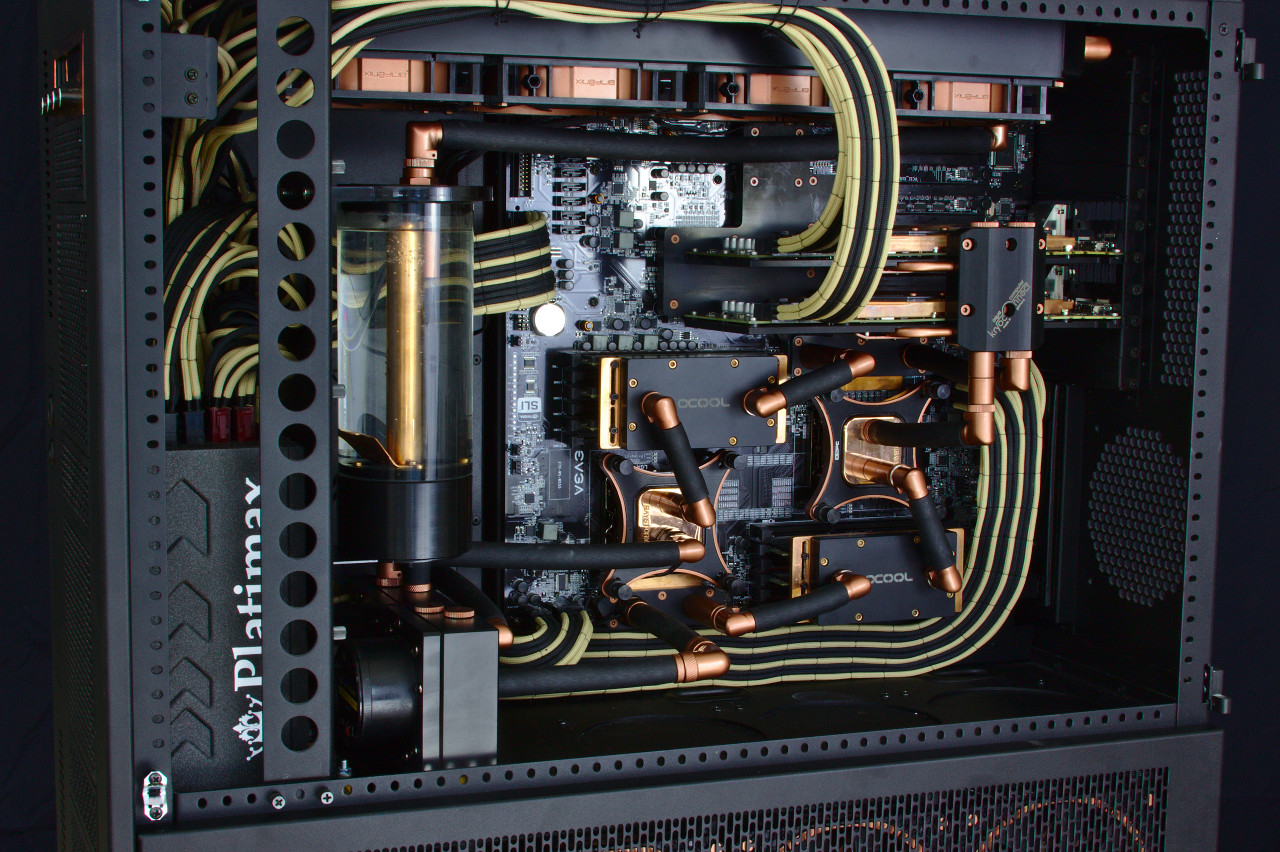
\includegraphics[width=120mm]{titlepic.jpg}

    \vfill

    \today\\
    Version 1.0.0
\end{titlingpage}
\frontmatter
\tableofcontents*

\mainmatter
\chapter{Text}
\lipsum[1]

\sffamily\lipsum[2]

\bfseries\lipsum[3]

\mdseries\ttfamily\lipsum[4]

\bfseries\ttfamily\lipsum[5]

\normalfont\scshape\lipsum[6]

\slshape\lipsum[7]

\scshape\lipsum[8]

\scslshape\lipsum[9]

\normalfont

\chapter{Tables}
\begin{table}
    \centering
    \caption{tabular inside float}
    \label{tab:float}
    \begin{tabular}{lll}
        \toprule
        \scshape Header 1 & \scshape Header 2 & \scshape Header 3 \\
        \midrule
        Content           & Content           & Content           \\
        Content           & Content           & Content           \\
        Content           & Content           & Content           \\
        Content           & Content           & Content           \\
        \bottomrule
    \end{tabular}
\end{table}

\lipsum[3]

\begin{center}
    \tabcaption{Tabular outside of float}
    \label{tab:outside}
    \begin{tabular}{lll}
        \toprule
        \scshape Header 1 & \scshape Header 2 & \scshape Header 3 \\
        \midrule
        Content           & Content           & Content           \\
        Content           & Content           & Content           \\
        Content           & Content           & Content           \\
        Content           & Content           & Content           \\
        \bottomrule
    \end{tabular}
\end{center}

\chapter{References and Hyperlinks}
This sentence refers to Table~\ref{tab:outside}.

This is a citation \cite{testitem}.

\href{https://hyperlink.com}{This is a hyperlink hiding behind text.}

\href{https://hyperlink.com}{\nolinkurl{https://hyperlink.com}}

\chapter{Sectional Headings}

This section illustrates the  style of \verb|\section|, \verb|\subsection| and
\verb|\subsubsection|.

\section{A Section}
\lipsum[2]

\subsection{A Subsection}
\lipsum[1]

\subsubsection{A subsubsection}
\lipsum[2]

\chapter{Code Listings}
\tikzset{external/export next=false}%
\begin{tcblisting}{%
        title=This Is a Code Listing,
        minted language=tex,
        listing side text,
        }
    \begin{tabular}{ll}
        a & a \\
        a & a \\
    \end{tabular}
\end{tcblisting}

\tikzset{external/export next=false}%
\begin{tcolorbox}[title=test]
    \lipsum[2]
\end{tcolorbox}

\tikzset{external/export next=false}%
\begin{tcolorbox}
    \lipsum[2]
\end{tcolorbox}

\chapter{Mathematics}

A numbered equation:
\begin{equation}
    y(x) = x^2 + 2x + 5
\end{equation}

An unnumbered equation:
\begin{equation*}
    x_{01,02} = -1 \pm 2j
\end{equation*}

An \verb|align| with some numbered and unnumbered lines:

\begin{align}
    \frac{\Phi}{i}
    & =
    \int_{0}^{\infty} \frac{dx}{x} \int_{0}^{l+m}
    \left[
        \frac{y dy}{\sqrt{x^2+y^2}} - \frac{(y-l) dy}{\sqrt{x^2+(y-l)^2}}
    \right]
    \nonumber
    \\
    &=
    \int_{0}^{\infty}
    \left[
        \sqrt{x^2 + (l+m)^2)} - \sqrt{x^2+l^2} - \sqrt{x^2+m^2}+x
    \right]
    \frac{dx}{x}
    \nonumber
    \\
    &=
    \Bigg[
        \sqrt{x^2 + (l+m)^2} - \sqrt{x^2+l^2} - \sqrt{x^2+m^2}
        \nonumber
        \\
        & ~~~~~~~~~   + x - l \cdot \log{\frac{l+m+\sqrt{x^2+(l+m)^2}}{l+\sqrt{x^2+l^2}}}
        \nonumber
        \\
        & ~~~~~~~~~   - m \cdot \log{\frac{l+m+\sqrt{x^2+(l+m)^2}}{m+\sqrt{x^2+l^2}}} ~
    \Bigg]_0^{\infty}
    \label{eq:mISL:2}
    \\
    & \approx
    \left[ l \cdot \log{\frac{l+m}{l}} + m \cdot \log{\frac{l+m}{m}} \right]
    \label{eq:mISL:3}
\end{align}


\cleardoublepage
\begin{titlingpage*}
    \fullhexpage{da2}{ct4}
    \begin{vplace}
        \flushright\Huge\bfseries\sffamily\appendixpagename
    \end{vplace}
\end{titlingpage*}
\appendix
\chapterstyle{alpenappendix}
\chapter{An Appendix Chapter}
\lipsum[1-3]

\chapter{Another Appendix Chapter with a Title That Requires Two Lines}
\lipsum[4-6]

\backmatter
\chapter{A Backmatter Chapter}
\lipsum[7-9]

\begin{thebibliography}{1}
    \bibitem{testitem}
        An Author, ``A Title``, 1979.
\end{thebibliography}
%% ============================================================== END CONTENT %
\end{document}
%</example>
% \fi
%^^A >>>
%
%^^A ------------------------------------------------------------------------- %
%^^A                                                  MULTI-LANGUAGE SUPPORT <<<
% \iffalse
%<*de>
\expandafter\newif\csname ifenglish\endcsname
\englishfalse
% \iffalse meta-comment
% -------------------------------------------------------- %
% Copyright (c) 2017 Raphael Frey rmfrey@runbox.com        %
% -------------------------------------------------------- %
%                                                          %
% This file  may be distributed and/or  modified under the %
% conditions of  the LaTeX Project Public  License, either %
% version 1.3c  of this  license or  (at your  option) any %
% later version. The latest version of this license is in: %
%                                                          %
%     http://www.latex-project.org/lppl.txt                %
%                                                          %
% and version 1.3c  or later is part  of all distributions %
% of LaTeX version 2008/05/04 or later.                    %
% -------------------------------------------------------- %
% \fi
%
%\CheckSum{0}
%
%
%^^A ------------------------------------------------------------------------- %
%^^A                                              DRIVER, PROVIDESCLASS ETC. <<<
% \iffalse
%<*driver>
\ProvidesFile{alpenthesis.dtx}
%</driver>
%<class>\NeedsTeXFormat{LaTeX2e}
%<class>\ProvidesClass{alpenthesis}%
%<*class>
    [2017/04/06 v0.0.1 PDF-LaTeX class for my thesis]
%</class>
%<*driver>
\expandafter\ifx\csname ifenglish\endcsname\relax
    \expandafter\newif\csname ifenglish\endcsname
    \englishtrue
\fi
\documentclass[a4paper,11pt,oneside]{ltxdoc}
\EnableCrossrefs
\CodelineIndex
\RecordChanges
% ----------------------------------------------- PACKAGES %
\usepackage[T1]{fontenc}
\usepackage[utf8]{inputenc}
\ifenglish
    \usepackage[english]{babel}
\else
    \usepackage[ngerman]{babel}
\fi
\usepackage{xcolor-solarized}
\usepackage[light,nott]{kpfonts}
\usepackage[scaled=0.8125]{DejaVuSansMono}
\usepackage{hypdoc}
\usepackage{tikz}
\usepackage{alpencolors}
\usepackage{booktabs}
\usepackage{imakeidx}
% ------------------------------------------ HELPER MACROS %
\newcommand*\pacname[1]{\textsf{#1}}
\newcommand*\code[1]{\texttt{#1}}
\newcommand*\athes{\pacname{alpenthesis}}
\newcommand*\memoir{\pacname{memoir}}
\begin{document} % ****************************** DOCUMENT %
    \DocInput{alpenthesis.dtx}
\end{document}
%</driver>
% \fi
%^^A >>>
%
%^^A ------------------------------------------------------------------------- %
%^^A                                                 GetFileInto, DoNotIndex <<<
% \GetFileInfo{alpenthesis.dtx}
% \DoNotIndex{\addtolength,\bfseries,\captiondelim,\captionnamefont}
% \DoNotIndex{\captiontitlefont,\checkandfixthelayout,\color,\Large}
% \DoNotIndex{\large,\LoadWithClassOptions,\maxsecnumdepth,\maxtocdepth}
% \DoNotIndex{\newcommand,\newfixedcaption,\pagestyle,\paperheight}
% \DoNotIndex{\paperwidth,\renewcommand,\RequirePackage,\setlength}
% \DoNotIndex{\setlrmarginsandblock,\setsecheadstyle,\setsubsecheadstyle}
% \DoNotIndex{\setsubsubsecheadstyle,\settrimmedsize,\settrims}
% \DoNotIndex{\setulmarginsandblock,\sffamily,\small,\stockaiii}
% \DoNotIndex{\stockwidth,\textsf,\texttt,\trimedge,\trimmarkscolor}
% \DoNotIndex{\trimtop}
% \DoNotIndex{\@chapapp,\addtodef,\afterchapskip,\afterchapternum}
% \DoNotIndex{\athes,\beforechapskip,\begin,\end}
% \DoNotIndex{\AT@bottomscreen,\chapnamefont,\chapnumfont}
% \DoNotIndex{\chapterheadstart,\chapternamenum,\chaptitlefont}
% \DoNotIndex{\edgewidth,\fadingIndex,\fi,\fill,\flushright,\foreach}
% \DoNotIndex{\globalcolorstrue,\height,\hspace,\HUGE,\includepdf}
% \DoNotIndex{\input,\iterstop,\iterstopvert,\j,\k,\LARGE,\leftTransp}
% \DoNotIndex{\MakeTextUppercase,\m,\makebox,\marginparsep,\marginparwidth}
% \DoNotIndex{\maxElementNumber,\midchapskip,\n,\newif,\newlength,\nobreak}
% \DoNotIndex{\numberOfHorizSides,\numberOfHorizElements,\offsetVert}
% \DoNotIndex{\par,\pgfkeysgetvalue,\pgfmathcos,\pgfmathmod,\pgfmathresult}
% \DoNotIndex{\pgfmathsetmacro,\pgfmathtruncatemacro,\pgfplotsset}
% \DoNotIndex{\printchaptername,\printchapternonum,\printchapternum}
% \DoNotIndex{\printchaptertitle,\x,\y,\resizebox}
% \DoNotIndex{\rightTransp,\rowtestcolor,\rule,\side,\spinemargin}
% \DoNotIndex{\textwidth,\thechapter,\thepage,\tikz,\tikzfading,\tikzset}
% \DoNotIndex{\usepackage,\usepgfplotslibrary,\usetikzlibrary,\vskip,\vspace}
%^^A>>>
%
%^^A ------------------------------------------------------------------------- %
%^^A                                                    TITLE, ABSTRACT, ToC <<<
% \author{Raphael Frey \\[1ex] \href{https://github.com/alpenwasser/}%
%                                     {\nolinkurl{https://github.com/alpenwasser/}}}
%
% \ifenglish
%   \title{The \athes\ Class\thanks{This document corresponds
%       to \athes~\fileversion, dated~\filedate.}}
%   \maketitle
%   \begin{abstract}
%        The \athes\  class is the  \LaTeX class I  wrote for my  thesis. It is
%        based on  the \memoir\  class and  is a  collection of  various custom
%        commands  and  configurations  to  suit my  personal  preferences  and
%        requirements. You may or  may not find some of it  useful, but keep in
%        mind that this is a class created  for a specific use case to cater to
%        a  select  few people's  preferences,  so  some  things may  not  seem
%        sensible or acceptable to you.
%
%        For  this  reason, the  class  does  not really  allow  for  a lot  of
%        customisation\footnotemark. It is primarily a ``fire-and-forget'' sort of affair.
%
%        \footnotetext{%
%            In principle,  most options and  commands from the  \memoir\ class
%            are present and  supported, but because this class loads  a lot of
%            packages  and preforms  a lot  of customization,  the results  may
%            sometimes  be undesired. I  have taken  no particular  precautions
%            when it comes to compatibility on  this level beyond what I needed
%            to make my personal configuration work as desired.}
%   \end{abstract}
% \else
%   \title{Die \athes-Klasse\thanks{Dieses Dokument entspricht
%          \athes~\fileversion, datiert~\filedate.}}
%   \maketitle
%   \begin{abstract}
%        Die \athes-Klasse  ist die \LaTeX-Klasse,  die ich f\"ur  meine Thesis
%        entwickelt habe,  aufbauend auf  der \memoir-Klasse. Sie  ist prim\"ar
%        eine Kollektion  von massgeschneiderten Befehlen  und Konfigurationen,
%        um   meine   pers\"onlichen   Bed\"urfnisse   und   Anforderungen   zu
%        erf\"ullen. Jemand  k\"onnte einen  Teil  davon allenfalls  n\"utzlich
%        finden. Man beachte  aber, dass diese Klasse  f\"ur einen spezifischen
%        Zweck f\"ur  einige wenige  Personen geschrieben  wurde. Somit m\"ogen
%        einige  Dinge  aus der  Sicht  der  geneigten Leserin  nicht  sinnvoll
%        implementiert sein.
%
%        Aus diesem  Grund ist  bei dieser  Klasse auch  nicht viel  Raum f\"ur
%        Konfiguration  vorgesehen\footnotemark. Es  ist  gr\"osstenteils  eine
%        ``fire-and-forget''-Angelegenheit.
%
%        \footnotetext{%
%            Im   Prinzip  werden   die  meisten   Optionen  und   Befehle  der
%            \pacname{memoir}-Klasse unterst\"utzt, aber  je nach Einstellungen
%            k\"onnten seltsame  Ergebnisse  auftreten,  da diese  Klasse viele
%            Packages l\"adt  und diverse Konfigurationen macht. Ich  habe hier
%            nicht explizit auf Kompatibilit\"at geachtet.}
%   \end{abstract}
% \fi
%
% \tableofcontents
%^^A >>>
%
%^^A ------------------------------------------------------------------------- %
%^^A                                                            INSTALLATION <<<
% \section{Installation}
% \label{sec:installation}
%
% \ifenglish
%    This section  deals with setting  up the \pacname{alpenthesis}  class and
%    setting up  a document with  it. Once you have generated  the \code{.cls}
%    class  file and  the \code{.pdf}  documentation (that  is: this  file, or
%    its  equivalent  in  another  language), or  have  received  those  files
%    from  somebody,  you  will   need  to  place  the  \code{alpenthesis.cls}
%    file  in  the  directory  of  your document  and  then  activate  it  via
%    |\documentclass{alpenthesis}|. See the \code{example.tex} for an example.
%
%    ^^A\inputminted[linenos=true,numbersep=4pt,fontsize=\footnotesize]{tex}{example.tex}
%   ^^A TODO: File structure tree with the needed files.
% \else
%    Dieser      Abschnitt      erkl\"art       die      Installation      der
%    \pacname{alpenthesis}-Klasse  und  erl\"autert,   wie  man  ein  Dokument
%    mit  ihr einrichtet. Nachdem  man  die \code{.cls}  Klassendatei und  die
%    Dokumentation  (dieses  Dokument,   oder  ein  anderssprachiges  Pendant)
%    generiert oder diese Dateien von  einer anderen Quelle erhalten hat, muss
%    man die Klassendatei \code{alpenthesis.cls} im selben Verzeichnis wie das
%    zu generierende Dokument platzieren und via |\documentclass{alpenthesis}|
%    aktivieren. Siehe  die  Datei   \code{example.tex},  welche  mitgeliefert
%    worden sein sollte.
% \fi
%^^A >>>
%
%^^A ------------------------------------------------------------------------- %
%^^A                                                          USER INTERFACE <<<
% \ifenglish
%    \section{User Interface}
%    \label{sec:user-interface}
% \else
%    \section{Benutzer-Interface}
%    \label{sec:user-interface}
% \fi
%
% |\documentclass\oarg{args}{alpenthesis}|\vspace{1em}
%
% \ifenglish
%    Loads  the  \athes\  class  with options  \meta{args}. Those  options  are
%    directly passed through to the  underlying \memoir\ class, so most options
%    for \memoir\  can be  specified. However, some may  be less  sensible than
%    others, given all the other configurations \athes\ makes.
%
%    If you require heavy customisation,  it is probably recommendable to start
%    off with the \memoir\ class itself as a base and build from there, relying
%    on its excellent documentation.
% \else
%    L\"adt    die    \athes-Klasse    mit    den    spezifizierten    Optionen
%    \meta{args}. Diese   Optionen   werden   direkt   an   die   unterliegende
%    \memoir-Klasse  weitergegeben. Somit  k\"onnen   beinahe  alle  f\"ur  die
%    \memoir-Klasse verf\"ugbaren Optionen  geladen werden. Man beachte jedoch,
%    dass  nicht unbedingt  alle  Optionen Sinn  machen,  da die  \athes-Klasse
%    selbst noch einige Konfigurationen vornimmt.
%
%    M\"ochte man  starke Individualisierungen  vornehmen, macht  es vermutlich
%    mehr Sinn, die  \memoir-Klasse direkt zu laden und  anhand der exzellenten
%    Dokumentation die gew\"unschte Konfiguration zu erstellen.
% \fi
% \DescribeMacro{\aiiistock}
% \DescribeMacro{\showtrimson}
% \DescribeMacro{\showtrimsoff}
% \ifenglish
%    Sets the  stock size to  A3 paper, keeping the  trimmed paper size  at A4,
%    vertically and  horizontally centered. Prints trim  marks for the  A4 page
%    centered on the A3 sheet.
%
%    To disable  trim marks,  you can  use the  |\showtrimsoff|. |\showtrimson|
%    will  enable them  again. Refer  to the  \memoir\  documentation for  more
%    information.
% \else
%    Setzt  die  Bogengr\"osse  auf  A3,  w\"ahrend  die  bedruckte  Seite  auf
%    A4  behalten wird.   Der  bedruckte Bereich  ist  vertikal und  horizontal
%    zentriert auf dem A3-Bogen. Druckt Markierungen um die A4-Seite.
%
%    Um  die  Markierungen zu  entfernen  kann  der |\showtrimsoff|-Befehl  von
%    \memoir\ benutzt werden. |\showtrimson| schaltet sie wieder ein. Siehe die
%    \memoir-Dokumentation.
% \fi
%
% \DescribeMacro{\hextrue}
% \DescribeMacro{\hexfalse}
% \ifenglish
%    In order to save time when compiling a document, the |\hexfalse| value can
%    be set in the preamble. This leads to the hexagon grind being omitted from
%    the chapter style.
%
%    Setting |\hextrue|  will enable the hexagons. This  lengthens compile time
%    significantly.
%
%    The principle is similar to the  |draft| option which is available in many
%    document classes and  packages. Personally I do not tend to  use that much
%    though because of  all the usual things which come  with |draft|, which is
%    why I decided to implement a separate command.
% \else
%    Um  Zeit  zu  sparen  beim   Kompilieren,  kann  man  |\hexfalse|  in  der
%    Pre\"aambel setzen. Dies f\"uhrt dazu,  dass die Hexagons im Kapitel-Style
%    nicht gedruckt werden.
%
%    Den  Wert   |\hextrue|  zu  setzen, aktiviert die  Hexagons. Dies
%    verl\"angert die Kompilierzeit bedeutend.
%
%    Das  Prinzip  ist  \"ahnlich  wie  die  in  vielen  Packages  und  Klassen
%    verf\"ugbare |draft|-Option. Da  ich diese  jedoch f\"ur  meinen Geschmack
%    im  Normalfall  etwas  viele  unerw\"unschte Seiteneffekte  hat,  ist  ein
%    unabh\"angiger Switch implementiert.
% \fi
%^^A >>>
%
% \StopEventually{\PrintIndex}
%^^A ------------------------------------------------------------------------- %
%^^A                                                          IMPLEMENTATION <<<
% \section{Implementation}
% \label{sec:implementation}
%
%^^A ---------------------------------------------- Loading the memoir Class <<<
% \ifenglish
%    \subsection{Loading the Base Class (\memoir)}
%    \label{subsec:memload}
%    The underlyng  class is  \memoir, and  all options  passed to  the \athes\
%    class are directly  passed on to \memoir\  via the |\LoadClassWithOptions|
%    command.
%
%    Additionally, the two hexagon configuration switches are defined.
% \else
%    \subsection{Laden der Basisklasse (\memoir)}
%    \label{subsec:memload}
%    Die  zugrundeliegende Klasse  ist \memoir. Alle  an \athes\  \"ubergebenen
%    Optionen   werden   direkt   an   die   \memoir-Klasse   \"ubergeben   via
%    |\LoadClassWithOptions|.
%
%    Im Weiteren werden  die beiden Konfigurations-Booloeans f\"ur die Hexagons
%    hier definiert.
% \fi
% \color{sqB}
%^^A Need the class guards to prevent the macro code from being included again
%^^A in example.tex and the German .tex file
% \iffalse
%<*class>
% \fi
%    \begin{macrocode}
\LoadClassWithOptions{memoir}
\newif\ifhex
\newif\ifpaper
%    \end{macrocode}
% \iffalse
%</class>
% \fi
% \color{black}
%^^A>>>
%^^A ---------------------------------------------- Fonts, inputenc, fontenc <<<
% \ifenglish
%    \subsection{General Configuration}
%    \label{subsec:general-config}
%    We choose  the \pacname{kpfonts}  Package for serif  and sans  serif fonts
%    with the  |light| option,  and \pacname{DejaVuSansMono} as  our typewriter
%    font. Also, we  ensure that we  can write our  source code files with UTF8
%    characters and have T1 font encoding for our output.
% \else
%    \subsection{Allgemeine Konfiguration}
%    \label{subsec:general-config}
%    Wir  w\"ahlen  \pacname{kpfonts} als  unsere  Schriftart  f\"ur Serif  und
%    Sans-Serif,  mit  der  |light|-Option,  und  \pacname{DejaVuSansMono}  als
%    unsere  Monospace-Schriftart. Wir  stellen   ebenfalls  sicher,  dass  wir
%    UTF8-Input in unserem  Quelltext haben k\"onnen und dass der  Output in T1
%    codiert wird.
% \fi
% \color{sqB}
% \iffalse
%<*class>
% \fi
%    \begin{macrocode}
\RequirePackage[rmx,nott,intlimits,sumlimits]{kpfonts}
\RequirePackage[scaled=0.8125]{DejaVuSansMono}
\RequirePackage[utf8]{inputenc}
\RequirePackage[T1]{fontenc}
%    \end{macrocode}
% \iffalse
%</class>
% \fi
% \color{black}
%^^A>>>
%^^A ------------------------------------------------ DOCUMENT COLOR PALETTE <<<
% \ifenglish
%    \subsection{Document Color Palette}
%    \label{subsec:colors}
%    We  define the  following  colors  as our  document  colors  in a  central
%    location.  This allows easy modification  of document colors while keeping
%    the entire document consistent.
% \else
%    \subsection{Farbpalette des Dokuments}
%    \label{subsec:colors}
%    Wir  definieren  die  folgenden  Farben  f\"ur  unser  Dokument  an  einer
%    zentralen Stelle.  Dies erlaubt es,  die Farbpalette des Dokuments einfach
%    zu  modifizieren  und  dabei  die   Farben  \"uber  das  gesamte  Dokument
%    konsistent zu behalten.
% \fi
% \color{sqB}
% \iffalse
%<*class|colors>
%^^A We  extract the  color information into  a package for  use in  the class
%^^A documentation.
%<colors>\ProvidesPackage{alpencolors}[2017/04/08 v1.0 color palette for alpenthesis]
% \fi
%    \begin{macrocode}
\RequirePackage{xcolor}
\globalcolorstrue
\newcommand*\testcolor[1]{\tikz \fill[#1] (0em,0ex) rectangle (2em,2ex);}
\newcommand*\rowtestcolor[1]{#1 & \tikz \fill[#1] (0em,0ex) rectangle (2em,2ex);}
%    \end{macrocode}
% \iffalse
%</class|colors>
% \fi
% \color{black}
% \ifenglish
%    \subsubsection{Dark-ish Colors}
%    \label{subsubsec:darkish}
% \else
%    \subsubsection{Eher Dunkle Farben}
%    \label{subsubsec:darkish}
% \fi
% \begin{center}
%     \small
%     \begin{tabular}{lllllllllll}
%         \toprule
%         \rowtestcolor{da0} &
%         \rowtestcolor{da1} &
%         \rowtestcolor{da2} &
%         \rowtestcolor{da3} &
%         \rowtestcolor{da4} \\
%         \bottomrule
%     \end{tabular}
% \end{center}
% \color{sqB}
% \iffalse
%<*class|colors>
% \fi
%    \begin{macrocode}
\definecolor{da0}{HTML}{002B36}  \definecolor{da1}{HTML}{073642}
\definecolor{da2}{HTML}{008080}  \definecolor{da3}{HTML}{800080}
\definecolor{da4}{HTML}{404040}
%    \end{macrocode}
% \iffalse
%</class|colors>
% \fi
% \color{black}
% \ifenglish
%    \subsubsection{Bright-ish Colors}
%    \label{subsubsec:brightish}
% \else
%    \subsubsection{Eher helle Farben}
%    \label{subsubsec:brightish}
% \fi
% \begin{center}
%     \small
%     \begin{tabular}{lllllllllll}
%         \toprule
%         \rowtestcolor{br0} &
%         \rowtestcolor{br1} &
%         \rowtestcolor{br2} \\
%         \bottomrule
%     \end{tabular}
% \end{center}
% \color{sqB}
% \iffalse
%<*class|colors>
% \fi
%    \begin{macrocode}
\definecolor{br0}{HTML}{BEB9AA}  \definecolor{br1}{HTML}{EEE8D5}
\definecolor{br2}{HTML}{FDF6E3}
%    \end{macrocode}
% \iffalse
%</class|colors>
% \fi
% \color{black}
% \ifenglish
%    \subsubsection{Contrast Color Palette}
%    \label{subsubsec:contrast}
% \else
%    \subsubsection{Kontrastfarben}
%    \label{subsubsec:contrast}
% \fi
% \begin{center}
%     \small
%     \begin{tabular}{lllllllllll}
%         \toprule
%         \rowtestcolor{ct0} &
%         \rowtestcolor{ct1} &
%         \rowtestcolor{ct2} &
%         \rowtestcolor{ct3} &
%         \rowtestcolor{ct4} \\
%         \rowtestcolor{ct5} &
%         \rowtestcolor{ct6} \\
%         \bottomrule
%     \end{tabular}
% \end{center}
% \color{sqB}
% \iffalse
%<*class|colors>
% \fi
%    \begin{macrocode}
\definecolor{ct0}{HTML}{CB4B16}  \definecolor{ct1}{HTML}{DC322F}
\definecolor{ct2}{HTML}{DC3682}  \definecolor{ct3}{HTML}{268BD2}
\definecolor{ct4}{HTML}{2AA198}  \definecolor{ct5}{HTML}{B58900}
\definecolor{ct6}{HTML}{859900}  \definecolor{sq0}{HTML}{F7FBFF}
%    \end{macrocode}
% \iffalse
%</class|colors>
% \fi
% \color{black}
% \ifenglish
%    \subsubsection{Sequential Color Palette}
%    \label{subsubsec:sequential}
% \else
%    \subsubsection{Sequentielle Farb-Palette}
%    \label{subsubsec:sequential}
% \fi
% \begin{center}
%     \small
%     \begin{tabular}{lllllllllll}
%         \toprule
%         \rowtestcolor{sq0} &
%         \rowtestcolor{sq1} &
%         \rowtestcolor{sq2} &
%         \rowtestcolor{sq3} &
%         \rowtestcolor{sq4} \\
%
%         \rowtestcolor{sq5} &
%         \rowtestcolor{sq6} &
%         \rowtestcolor{sq7} &
%         \rowtestcolor{sq8} &
%         \rowtestcolor{sq9} \\
%
%         \rowtestcolor{sqA} &
%         \rowtestcolor{sqB} &
%         \rowtestcolor{sqC} \\
%         \bottomrule
%     \end{tabular}
% \end{center}
% \color{sqB}
% \iffalse
%<*class|colors>
% \fi
%    \begin{macrocode}
\definecolor{sq1}{HTML}{EFF3FF}  \definecolor{sq2}{HTML}{DECDF7}
\definecolor{sq3}{HTML}{C6DBEF}  \definecolor{sq4}{HTML}{BDD7E7}
\definecolor{sq5}{HTML}{9ECAE1}  \definecolor{sq6}{HTML}{6BAED6}
\definecolor{sq7}{HTML}{4292C6}  \definecolor{sq8}{HTML}{3182BD}
\definecolor{sq9}{HTML}{2171B5}  \definecolor{sqA}{HTML}{08519C}
\definecolor{sqB}{HTML}{084594}  \definecolor{sqC}{HTML}{08306B}
%    \end{macrocode}
% \iffalse
%</class|colors>
% \fi
% \color{black}
% \ifenglish
%    \subsubsection{Divergent color palette}
%    \label{subsubsec:divergent}
% \else
%    \subsubsection{Divergierende Farb-Palette}
%    \label{subsubsec:divergent}
% \fi
% \begin{center}
%     \small
%     \begin{tabular}{lllllllllll}
%         \toprule
%         \rowtestcolor{dv-7} &
%         \rowtestcolor{dv-6} &
%         \rowtestcolor{dv-5} &
%         \rowtestcolor{dv-4} &
%         \rowtestcolor{dv-3} \\
%
%         \rowtestcolor{dv-2} &
%         \rowtestcolor{dv-1} &
%         \rowtestcolor{dv+0} &
%         \rowtestcolor{dv+1} &
%         \rowtestcolor{dv+2} \\
%
%         \rowtestcolor{dv+3} &
%         \rowtestcolor{dv+4} &
%         \rowtestcolor{dv+5} &
%         \rowtestcolor{dv+6} &
%         \rowtestcolor{dv+7} \\
%         \bottomrule
%     \end{tabular}
% \end{center}
% \color{sqB}
% \iffalse
%<*class|colors>
% \fi
%    \begin{macrocode}
\definecolor{dv-7}{HTML}{8E0152} \definecolor{dv-6}{HTML}{C51B7D}
\definecolor{dv-5}{HTML}{D01C8B} \definecolor{dv-4}{HTML}{DE77AE}
\definecolor{dv-3}{HTML}{E9A3C9} \definecolor{dv-2}{HTML}{F1B6DA}
\definecolor{dv-1}{HTML}{FDE0EF} \definecolor{dv+0}{HTML}{F7F7F7}
\definecolor{dv+1}{HTML}{D1E5F0} \definecolor{dv+2}{HTML}{92C5DE}
\definecolor{dv+3}{HTML}{67A9CF} \definecolor{dv+4}{HTML}{4393C3}
\definecolor{dv+5}{HTML}{0571B0} \definecolor{dv+6}{HTML}{2166AC}
\definecolor{dv+7}{HTML}{053061}
%    \end{macrocode}
% \iffalse
%</class|colors>
% \fi
% \color{black}
% \ifenglish
%    \subsubsection{Qualitative Color Palette}
%    \label{subsubsec:qualitative}
% \else
%    \subsubsection{Qualitative Farb-Palette}
%    \label{subsubsec:qualitative}
% \fi
% \begin{center}
%     \small
%     \begin{tabular}{lllllllllll}
%         \toprule
%         \rowtestcolor{q0} &
%         \rowtestcolor{q1} &
%         \rowtestcolor{q2} &
%         \rowtestcolor{q3} &
%         \rowtestcolor{q4} \\
%
%         \rowtestcolor{q5} &
%         \rowtestcolor{q6} &
%         \rowtestcolor{q7} \\
%         \bottomrule
%     \end{tabular}
% \end{center}
% \color{sqB}
% \iffalse
%<*class|colors>
% \fi
%    \begin{macrocode}
\definecolor{q0}{named}{ct3}   \definecolor{q1}{named}{sqB}
\definecolor{q2}{named}{ct2}   \definecolor{q3}{named}{da3}
\definecolor{q4}{HTML}{FEC44F} \definecolor{q5}{named}{ct0}
\definecolor{q6}{HTML}{80EA82} \definecolor{q7}{HTML}{2E7D32}
%    \end{macrocode}
% \iffalse
%</class|colors>
% \fi
% \color{black}
%^^A NOTE: each \rowtestcolor command requires two columns!
%^^A >>>
%^^A --------------------------------------------------- TikZ, PGF, PGFPLOTS <<<
% \ifenglish
%    \subsection{Ti\emph{k}Z, \textsc{pgfplots}}
%    \label{subsec:tikz-pgfplots}
% \else
%    \subsection{Ti\emph{k}Z, \textsc{pgfplots}}
%    \label{subsec:tikz-pgfplots}
% \fi
% \color{sqB}
% \iffalse
%<*class>
% \fi
%    \begin{macrocode}
\RequirePackage{tikz}
\usetikzlibrary{calc}
\usetikzlibrary{fadings}
\RequirePackage{pgfplots}
\pgfplotsset{compat=1.14}
\usepgfplotslibrary{external}
\tikzexternalize[prefix=cache/,optimize command away=\includepdf]
%    \end{macrocode}
% \iffalse
%</class>
% \fi
% \color{black}
%^^A >>>
%^^A -------------------------------------------------- HEXAGON CALCULATIONS <<<
% \ifenglish
%    \subsection{Hexagon Calculations}
%    \label{subsec:hexagon-calcs}
%    In this section,  the various required calculations for  the hexagon grids
%    are made. The basis is the number  of hexagons sides (not hexagons!) which
%    are to fit into one page width. Going  from there, the height of a hexagon
%    as well as the number of rows and columns are calculated.
% \else
%    \subsection{Berechnungen f\"ur Hexagons}
%    \label{subsec:hexagon-calcs}
%    An  dieser   Stelle  werden   diverse  Berechnungen  f\"ur   die  Hexagons
%    ausgef\"uhrt.  Grundlage ist die  Anzahl Hexagon-Seitenl\"angen (nicht die
%    Anzahl  Hexagons!), welche  in eine  Seitenbreite passt. Darauf  basierend
%    werden die halbe H\"ohe eines Hexagons sowie die Anzahl Spalten und Zeilen
%    berechnet.
% \fi
% \color{sqB}
% \iffalse
%<*class>
% \fi
%    \begin{macrocode}
\pgfmathsetmacro\AT@paperwidth{21}
\pgfmathsetmacro\AT@paperheight{29.7}
\pgfmathsetmacro\AT@numberOfSidesHorizontally{22}
\pgfmathsetmacro\AT@side
    {\AT@paperwidth / \AT@numberOfSidesHorizontally}
\pgfmathtruncatemacro\AT@totCols
    {0.666667 * \AT@numberOfSidesHorizontally + 1}
\pgfmathcos{30}
\pgfmathsetmacro\AT@height
    {\pgfmathresult * \AT@side}
\pgfmathtruncatemacro\AT@numberOfHeightsVertically
    {\AT@paperheight / \AT@height}
\pgfmathtruncatemacro\AT@totRows
    {0.5 * \AT@numberOfHeightsVertically + 1}
\pgfmathtruncatemacro\AT@totRowsChap
    {0.1333 * \AT@numberOfHeightsVertically + 1}
%    \end{macrocode}
% \iffalse
%</class>
% \fi
% \color{black}
% \ifenglish
%    If the print version is to be generated, a uniform color for each hexagon,
%    depending on its horizontal and vertical position, is calculated:
% \else
%    Falls  die Druckversion  erstellt werden  soll, wird  eine uniforme  Farbe
%    f\"ur  jedes Hexagon,  abh\"angig von  seiner horizontalen  und vertikalen
%    Position, generiert:
% \fi
% \color{sqB}
% \iffalse
%<*class>
% \fi
%    \begin{macrocode}
\AtBeginDocument{%
    \ifpaper
        \foreach \y in {0,...,\AT@totRowsChap} {%
            \foreach \x in {0,...,\AT@totCols}{%
                \pgfmathsetmacro\mix
                    {100 * \x / \AT@totCols}%
                \pgfmathsetmacro\mixvert
                    {100 * \y / \AT@totRowsChap}%
                \colorlet{hex-\x}{white!\mix!br0}%
                \colorlet{hex-\x-\y}{white!\mixvert!hex-\x}%
                \colorlet{hexframecol-\x}{white!\mix!br2}%
                \colorlet{hexframecol-\x-\y}
                    {white!\mixvert!hexframecol-\x}%
                \colorlet{chapcol-\x}{dv-4!\mix!dv-7}%
                \colorlet{chapcol-\x-\y}
                    {dv-2!\mixvert!chapcol-\x}%
                \colorlet{appcol-\x}{ct4!\mix!da2}%
                \colorlet{appcol-\x-\y}{white!\mixvert!appcol-\x}%
            }%
        }%
%    \end{macrocode}
% \iffalse
%</class>
% \fi
% \color{black}
% \ifenglish
%    For the  electronic version,  fadings are used  instead. Unfortunately, we
%    cannot simply have one global fading  which applies to all hexagons (since
%    each hexagon is  a single path)\footnotemark, so one  fading is calculated
%    for each  hexagon based  on its  horizontal position. The  vertical fading
%    effect is later achieved by  overlaying a white-to-transparent screen from
%    the grid's bottom edge. Maybe one day I'll figure out how to combine these
%    into one single and nice step.
%
%    \footnotetext{%
%        Or more accurately: I  have not been able to find  a way to accomplish
%        this.}
% \else
%    F\"ur die elektronische Version werden stattdessen Fadings benutzt. Leider
%    kann  nicht  einfach   ein  globales  Fading  definiert   und  \"uber  das
%    gesamte  Gitter  gelegt  werden  (da   jedes  einzelne  Hexagon  ein  Pfad
%    ist)\footnotemark, deshalb  wird f\"ur jedes Hexagon  ein Fading bestimmt,
%    abh\"angig  von   der  horizontalen  Position  im   Gitter. Der  vertikale
%    Fading-Effekt  wird  mit   einem  weiss-zu-transparenten  Fading  erzeugt,
%    welches dem gesamten Gitter  von unten \"uberlagert wird. Vielleicht finde
%    ich  eines  Tages eine  clevere  Variante,  die  beiden Effekte  in  einen
%    einzelnen, eleganten Schritt zu kombinieren.
%
%    \footnotetext{%
%        Oder genauer  gesagt: Ich habe  bisher nicht herausgefunden,  wie dies
%        m\"oglich w\"are.}
% \fi
% \color{sqB}
% \iffalse
%<*class>
% \fi
%    \begin{macrocode}
    \else
        \foreach \x in {0,...,\AT@totCols}{%
            \pgfmathsetmacro\leftTransp
                {100 *  \x    / \AT@totCols}%
            \pgfmathsetmacro\rightTransp
                {100 * (\x+1) / \AT@totCols}%
            \tikzfading[%
                name=hexfade \x,
                right color=transparent!\rightTransp,
                left color=transparent!\leftTransp]%
        }%
    \fi
}
\newcommand\AT@providehexagonpath[3]{%
    ($(current page.north west) +
        (1.5 * #1 * \AT@side,
            #3 * \AT@height - #2 * 2 * \AT@height)$)
    -- ++(   0:\AT@side)
    -- ++( -60:\AT@side)
    -- ++(-120:\AT@side)
    -- ++(-180:\AT@side)
    -- ++(-240:\AT@side) -- cycle;
}
%    \end{macrocode}
% \iffalse
%</class>
% \fi
% \color{black}
%^^A >>>
%^^A ------------------------------------------ HEXAGON FULL PAGE BACKGROUND <<<
% \ifenglish
%    \subsection{Hexagon Page Background}
%    \label{subsec:hexagon-background}
% \else
%    \subsection{Hexagon Seitenhintergrund}
%    \label{subsec:hexagon-background}
% \fi
% \color{sqB}
% \iffalse
%<*class>
% \fi
%    \begin{macrocode}
\newcommand\fullhexpage[2]{%
    \ifhex
        \tikzset{external/export next=false}%
        \begin{tikzpicture}[remember picture,overlay,x=1cm,y=1cm]
            \path[clip]
                (current page.north west)
                rectangle
                (current page.south east);
            \foreach \y in {0,...,\AT@totRows} {%
                \foreach \x in {0,...,\AT@totCols} {%
                    \pgfmathsetmacro\AT@isodd{mod(\x,2)}
                    \fill[fill=br2,draw=br1]
                        \AT@providehexagonpath{\x}{\y}{\AT@isodd}
                }
            }
            % Create vertical contrast bar on left side.
            % Put it inside scope for clipping.
            \begin{scope}
                \path[clip]
                    (current page.north west)
                    rectangle
                    ($(current page.south west) +
                        (3.5 * \AT@side,0)$);
                \foreach \y in {0,...,\AT@totRows} {%
                    \foreach \x in {0,...,2} {%
                        \pgfmathsetmacro\AT@isodd{mod(\x,2)}
                        \fill[fill=#1,draw=#2]
                            \AT@providehexagonpath{\x}{\y}{\AT@isodd}
                    }
                }
            \end{scope}
        \end{tikzpicture}%
    \fi
}
%    \end{macrocode}
% \iffalse
%</class>
% \fi
% \color{black}
%^^A>>>
%^^A ------------------------------------------------------------- tcolorbox <<<
% \ifenglish
%    \subsection{\pacname{tcolorbox}}
%    \label{subsec:tcolorbox}
%
%    Keeping with the theme of angled things, we define an octagon shape
%    as the surrounding shape for \pacname{tcolorbox}.
% \else
%    \subsection{\pacname{tcolorbox}}
%    \label{subsec:tcolorbox}
%
%    Um zum allgemeinen Thema der gewinkelten Dinge zu passen, wird ein Oktagon
%    als Form f\"ur den Rahmen der \pacname{tcolorbox}-Elemente definiert.
% \fi
% \color{sqB}
% \iffalse
%<*class>
% \fi
%    \begin{macrocode}
\RequirePackage{tcolorbox}
\tcbuselibrary{minted}
\tcbuselibrary{skins}
\tcbset{%
    colback=br2,
    coltitle=br2,
    colframe=da1,
    fonttitle=\sffamily,
    minted options={autogobble},
    enhanced,
    frame code={
        \draw[very thick]
               ([xshift=-3mm,yshift=+1mm]frame.north east)
            -- ([xshift=+0mm,yshift=-2mm]frame.north east)
            -- ([xshift=+0mm,yshift=+2mm]frame.south east)
            -- ([xshift=-3mm,yshift=-1mm]frame.south east)
            -- ([xshift=+3mm,yshift=-1mm]frame.south west)
            -- ([xshift=-0mm,yshift=+2mm]frame.south west)
            -- ([xshift=-0mm,yshift=-2mm]frame.north west)
            -- ([xshift=+3mm,yshift=+1mm]frame.north west)
            -- cycle;
    },
    interior titled code={%
        \path[tcb fill interior]
               ([xshift=-2.7mm,yshift=+1.3mm]interior.north east)
            -- ([xshift=+0.3mm,yshift=-1.7mm]interior.north east)
            -- ([xshift=+0.3mm,yshift=+1.7mm]interior.south east)
            -- ([xshift=-2.7mm,yshift=-1.3mm]interior.south east)
            -- ([xshift=+2.7mm,yshift=-1.3mm]interior.south west)
            -- ([xshift=-0.3mm,yshift=+1.7mm]interior.south west)
            -- ([xshift=-0.3mm,yshift=-1.7mm]interior.north west)
            -- ([xshift=+2.7mm,yshift=+1.3mm]interior.north west)
            -- cycle;
    },
    interior code={%
        \path[tcb fill interior]
               ([xshift=-2.7mm,yshift=+1.3mm]interior.north east)
            -- ([xshift=+0.3mm,yshift=-1.7mm]interior.north east)
            -- ([xshift=+0.3mm,yshift=+1.7mm]interior.south east)
            -- ([xshift=-2.7mm,yshift=-1.3mm]interior.south east)
            -- ([xshift=+2.7mm,yshift=-1.3mm]interior.south west)
            -- ([xshift=-0.3mm,yshift=+1.7mm]interior.south west)
            -- ([xshift=-0.3mm,yshift=-1.7mm]interior.north west)
            -- ([xshift=+2.7mm,yshift=+1.3mm]interior.north west)
            -- cycle;
    },
    title code={%
        \path[tcb fill frame]
               ([xshift=-3mm,yshift=+1mm]frame.north east)
            -- ([xshift=+0mm,yshift=-2mm]frame.north east)
            -- ([xshift=+0.3mm,yshift=-2mm]interior.north east)
            -- ([xshift=-3mm,yshift=+1mm]interior.north east)
            -- ([xshift=+3mm,yshift=+1mm]interior.north west)
            -- ([xshift=-0.3mm,yshift=-2mm]interior.north west)
            -- ([xshift=-0mm,yshift=-2mm]frame.north west)
            -- ([xshift=+3mm,yshift=+1mm]frame.north west)
            -- cycle;
    }
}
%    \end{macrocode}
% \iffalse
%</class>
% \fi
% \color{black}
%^^A >>>
%^^A ------------------------------------ OTHER PACKAGES WOTHOUT MUCH CONFIG <<<
% \ifenglish
%    \subsection{Other Packages}
%    \label{subsec:other-packages}
% \else
%    \subsection{Andere Packages}
%    \label{subsec:other-packages}
% \fi
% \color{sqB}
% \iffalse
%<*class>
% \fi
%    \begin{macrocode}
\RequirePackage[%
    pdfauthor=alpenwasser,
    pdfsubject={LaTeX document design},
    pdftitle={alpenwasser's thesis},
    bookmarksnumbered=true,
    pdfkeywords={LaTeX,design,alpenwasser,thesis,class,hexagons},
    colorlinks=true,
    linkcolor=sqB,
    citecolor=ct4,
    urlcolor=dv-6]{hyperref}
\RequirePackage[english]{babel}
\RequirePackage{amsmath}
\RequirePackage[separate-uncertainty=true]{siunitx}
\RequirePackage{counttexruns}
%    \end{macrocode}
% \iffalse
%</class>
% \fi
% \color{black}
%^^A >>>
%^^A --------------------------------------------------------- MEMOIR CONFIG <<<
%
%^^A -------------------------------------------------------- General Config <<<
% \ifenglish
%   \subsection{\memoir\ Configuration}
%   \label{subsec:memconfig}
%   \subsubsection{General Configuration}
%   \label{subsubsec:memoir:general-config}
% \else
%   \subsection{\memoir-Konfiguration}
%   \label{subsec:memconfig}
%   \subsubsection{Allgemeine Konfiguration}
%   \label{subsubsec:memoir:general-config}
% \fi
% \color{sqB}
% \iffalse
%<*class>
% \fi
%    \begin{macrocode}
\maxsecnumdepth{subsubsection}
\maxtocdepth{subsubsection}
\chapterstyle{veelo}
%    \end{macrocode}
% \iffalse
%</class>
% \fi
% \color{black}
%^^A>>>
%^^A ----------------------------------------------------------- Page Layout <<<
% \ifenglish
%     \subsubsection{Page Layout}
%     \label{subsubsec:page-layout}
% \else
%     \subsubsection{Seiten-Layout}
%     \label{subsubsec:page-layout}
% \fi
% \color{sqB}
% \iffalse
%<*class>
% \fi
%    \begin{macrocode}
\newcommand\aiiistock{%
    \stockaiii
    \settrimmedsize{297mm}{210mm}{*}
    \setlength{\trimtop}{\stockheight}
    \addtolength{\trimtop}{-\paperheight}
    \setlength{\trimedge}{\stockwidth}
    \addtolength{\trimedge}{-\paperwidth}
    \settrims{0.5\trimtop}{0.5\trimedge}
    \renewcommand*{\trimmarkscolor}{\color{red}}
    \showtrimson
    \checkandfixthelayout
}
\showtrimsoff
\setlrmarginsandblock{0.142857111\paperwidth}{0.190476190\paperwidth}{*}
\setulmarginsandblock{0.111111111\paperheight}{*}{1.5}%
\checkandfixthelayout
%    \end{macrocode}
% \iffalse
%</class>
% \fi
% \color{black}
%^^A>>>
%^^A -------------------------------------------- Sectional Title Formatting <<<
% \ifenglish
%    \subsubsection{Sectional Title Fonts and Styles} ^^A ---- Sec Title Fonts %
%    \label{subsubsec:title-fonts}
%    Sets font styles and other stylistic attributes for headings.
% \else
%    \subsubsection{Schriftarten und Stil f\"ur Titel von Abschnitten}
%    \label{subsubsec:title-fonts}
%    Definiert Schriftarten und andere Stil-Attribute f\"ur \"Uberschriften.
% \fi
% \color{sqB}
% \iffalse
%<*class>
% \fi
%    \begin{macrocode}
\setsecheadstyle{\color{sqB}\Large\bfseries\sffamily}
\setsubsecheadstyle{\color{sqB}\large\bfseries\sffamily}
\setsubsubsecheadstyle{\color{sqB}\bfseries\sffamily}
\addtodef{\printchaptername}{\color{sqB}}{}
%    \end{macrocode}
% \iffalse
%</class>
% \fi
% \color{black}
%^^A>>>
%^^A --------------------------------------------------- Headers and Footers <<<
% \ifenglish
%   \subsubsection{Headers and Footers}
%   \label{subsubsec:headers-footers}
% \else
%   \subsubsection{Kopf- und Fusszeilen}
%   \label{subsubsec:headers-footers}
% \fi
% \color{sqB}
% \iffalse
%<*class>
% \fi
%    \begin{macrocode}
\pagestyle{headings}
%    \end{macrocode}
% \iffalse
%</class>
% \fi
% \color{black}
%^^A>>>
%^^A -------------------------------------------------------------- Captions <<<
% \ifenglish
%   \subsubsection{Captions}
%   \label{subsubsec:captions}
% \else
%   \subsubsection{Legenden}
%   \label{subsubsec:captions}
% \fi
% \color{sqB}
% \iffalse
%<*class>
% \fi
%    \begin{macrocode}
\captionnamefont{\bfseries\small}
\captiontitlefont{\small}
\captiondelim{: }
% Captions for use outside of floats
\newfixedcaption{\figcaption}{figure}
\newfixedcaption{\tabcaption}{table}
%    \end{macrocode}
% \iffalse
%</class>
% \fi
% \color{black}
%^^A>>>
%^^A -------------------------------------------------------- Chapter Styles <<<
% \color{black}
% \ifenglish
%   \subsubsection{Chapter Style}
%   \label{subsubsec:chapterstyle}
%    The chapters are styled with grid of hexagons whose color is faded towards
%    the right sight of the page and towards the bottom. There are two versions
%    of  this  mechanisms: One for  printing,  activated  via the  |\papertrue|
%    switch, and  one for  the electronic document  version, activated  via the
%    |\paperfalse| switch (or no switch at all).
%
%    The  reason for  the two  implementation is  that the  electronic  version
%    uses  fadings  and   transparency,  which  can  cause   issues  with  some
%    printers\footnotemark.  Therefore,  instead of fadings, the  print version
%    uses  hexagons which  have slightly  differing colors, but each  hexagon's
%    color is  uniform. This does  not look  quite as nice  on the  screen, but
%    printing results have been satisfactory for  me so far, though obviously I
%    would prefer the faded version to just work. Your mileage may vary.
%
%    \footnotetext{%
%        I have had a  Canon printer do a hard reset while  trying to print the
%        faded version from a USB  stick plugged into the  printer. Our Kyocera
%        printer simply  printed a black bar  instead of hexagons when  I tried
%        doing the same.}
%
%    The  |\AT@hexagons|  command prints  the  background  hexagon grid  for
%    numbered chapters, appendix chapters and unnumbered chapters.
% \else
%   \subsubsection{Kapitel-Stil}
%   \label{subsubsec:chapterstyle}
%    Die  Kapitel  werden  mit  einem  Gitter  von  Hexagons  dekoriert,  deren
%    Farbe  gegen rechts  und gegen  unten  verblasst in  Richtung weiss  (bzw.
%    transparent). Es gibt  zwei Verianten  dieses Mechanismus: Eine  f\"ur die
%    elektronische  Version,  welche  die   Standardeinstellung  ist  oder  mit
%    |\paperfalse| explizit aktiviert  werden kann, und eine  Version f\"ur den
%    Druck, welche mit |\papertrue| aktiviert wird.
%
%    Der  Grund   f\"ur  die   zwei  unterschiedlichen   Implementationen  ist,
%    dass   Drucker    h\"aufig   Probleme   mit   Transparenz    und   Fadings
%    haben\footnotemark. Die   Druckversion   benutzt   daher   statt   Fadings
%    unterschiedliche  Farben f\"ur  die Hexagons,  wobei jedoch  jedes Hexagon
%    eine  uniforme Farbe  hat. Dies  sieht  nicht ganz  so  nett  aus auf  dem
%    Bildschirm,  aber  Druckresultate  waren   bisher  ganz  gut,  obwohl  ich
%    es  nat\"urlich  bevorzugen  w\"urde,  wenn  die  Fading-Variante  einfach
%    funktionieren w\"urde. Your mileage may vary.
%
%    \footnotetext{%
%        Ich habe  bei einem Canon-Drucker  erlebt, dass er einen  harten Reset
%        machte,  als ich  versuchte, das  Dokument mit  Transparenz von  einem
%        USB-Stick  zu drucken,  der direkt  am Drucker  eingesteckt war. Unser
%        Kyocera-Drucker  druckte  statt  der   Hexagons  einach  einen  dicken
%        schwarzen Balken beim selben Versuch.}
%
%    Der  |\AT@hexagons|-Befehl druckt  das  Hintergrundgitter mit  Hexagons
%    f\"ur numerierte und unnumerierte Kapitel sowie Kapitel im Appendix.
% \fi
% \color{sqB}
% \iffalse
%<*class>
% \fi
%    \begin{macrocode}
\newcommand\AT@hexagons{%
    \tikzset{external/export next=false}%
    \begin{tikzpicture}[remember picture,overlay,x=1cm,y=1cm]
%    \end{macrocode}
% \iffalse
%</class>
% \fi
% \color{black}
% \ifenglish
%    Remove anything that is outside the page.
% \else
%    Allen Inhalt entfernen, der ausserhalb der Seite liegt.
% \fi
% \color{sqB}
% \iffalse
%<*class>
% \fi
%    \begin{macrocode}
        \ifpaper
            \path[clip]
                (current page.north west)
                rectangle
                ($(current page.north east) + (-0pt,-11 * \AT@height)$);
        \else
            \path[clip]
                (current page.north west)
                rectangle
                ($(current page.north east) + (-0pt,-11 * \AT@height)$);
        \fi
%    \end{macrocode}
% \iffalse
%</class>
% \fi
% \color{black}
% \ifenglish
%    The outer loop iterates over the  rows, while the inner loop iterates over
%    the columns. Because the hexagons are offset by one |\AT@height| in the
%    vertical direction between  even and odd columns, we must  for each column
%    determine if it is an even or odd one, and then offset it, or not.
%
%    Also,  depending   on  whether   we're  in   |\papertrue|  mode   or  not,
%    we   either  use   the   fadings   or  uniform   colors   as  defined   in
%    Section~\ref{subsec:hexagon-calcs}.
% \else
%    Die  \"aussere   Schleife  iteriert  \"uber  die   Zeilen,  w\"ahrend  die
%    innere Schleife  \"uber die  Spalten iteriert. Weil  die Hexagons  um eine
%    |\@AT@height| versetzt sind, abh\"angig davon,  ob sie in einer geraden
%    oder ungeraden Spalte sind, muss f\"ur jede Spalte bestimmt werden, ob sie
%    gerade oder ungerade ist, um sie dann entsprechend zu versetzen, oder eben
%    nicht.
%
%    Im  Weiteren  werden,  abh\"angig   davon  ob  wir  im  |\papertrue|-Modus
%    sind oder  nicht, die in  Abschnitt~\ref{subsec:hexagon-calcs} definierten
%    Fadings oder Farben benutzt.
% \fi
% \color{sqB}
% \iffalse
%<*class>
% \fi
%    \begin{macrocode}
        \foreach \y in {0,...,\AT@totRowsChap} {%
            \foreach \x in {0,...,\AT@totCols} {%
                \pgfmathsetmacro\AT@isodd{mod(\x,2)}
                \ifpaper
                    \path[fill=hex-\x-\y,draw=hexframecol-\x-\y]
                \else
                    \path[fill=br0,draw=br1,path fading=hexfade \x]
                \fi
                    \AT@providehexagonpath{\x}{\y}{\AT@isodd}
            }%
        }%
    \end{tikzpicture}%
}
%    \end{macrocode}
% \iffalse
%</class>
% \fi
% \color{black}
%
% \DescribeMacro{\AT@numhexagons}%
% \ifenglish
%    The |\AT@numhexagons| command prints a number of hexagon colored in
%    a  contrast  color. The number  of  hexagons  corresponds to  the  current
%    chapter  number. This command  is  therefore not  executed for  unnumbered
%    chapters.
%
%    The  mechanism for  the offset  based  on even  or odd  column numbers  is
%    identical to the one used in the background hexagon grid.
%
%    The command requires four arguments:\newline\color{sqB}
%    |\AT@numhexagons|\marg{1,A}\marg{chapter,appendix}\marg{appcol,chapcol}\marg{color}
%    \color{black}
%    The  syntax  \meta{X,Y} indicates  that  either  \emph{X} or  \emph{Y}  is
%    required.
%    \begin{description}
%        \item[\normalfont\color{sqB}\meta{1,A}:] The  starting  point for  the
%            iteration  of  the  chapter  number. |1|  for  regularly  numbered
%            chapters,  |A| for  appendix chapters. Must  be one  of these  two
%            choices.
%
%        \item[\normalfont\color{sqB}\meta{chapter,appendix}:] Is used  to look
%            up the randomly  generated coordinates in the PGF key  trey in the
%            |randInts.tex| file. Must be one of these two choices.
%
%        \item[\normalfont\color{sqB}\meta{appcol,chapcol}:] The  color  prefix
%            string for  appendix and numbered chapters,  respectively, for the
%            paper version. Must be one of these two choices.
%
%        \item[\normalfont\color{sqB}\meta{color}:] The  color which  is to  be
%            used to fill  the contrast hexagons in the case  of the electronic
%            version. Can be any defined color.
%    \end{description}
% \else
%    Der  |\AT@numhexagons|-Befehl druckt  Hexagons in  einer Kontrastfarbe,
%    deren  Anzahl der  aktuellen Kapitelnummer  entspricht. F\"ur unnumerierte
%    Kapitel wird dieser Befehl nat\"urlich nicht ausgef\"uhrt.
%
%    Der  Mechanismus  zur Bestimmung  der  Versetzung  abh\"angig von  gerader
%    respektive ungerader  Spalten-Nummer ist identisch zu  demjenigen, welcher
%    f\"ur das Hintergrund-Grid verwendet wird.
%
%    Der Befehl ben\"otigt vier  Parameter:\newline\color{sqB}
%    |\AT@numhexagons|\marg{1,A}\marg{chapter,appendix}\marg{appcol,chapcol}\marg{color}
%    \color{black}
%    Die Syntax  \meta{X,Y} signalisiert, dass entweder  \emph{X} oder \emph{Y}
%    angegeben werden muss.
%    \begin{description}
%        \item[\normalfont\color{sqB}\meta{1,A}:] Der   Startpunkt  f\"ur   die
%            Iteration der Kapitelzahl.  |1|  f\"ur normal nummerierte Kapitel,
%            |A| f\"ur  Kapitel im Anhang.   Muss eine dieser  beiden Varianten
%            sein.
%
%        \item[\normalfont\color{sqB}\meta{chapter,appendix}:] Wird benutzt, um
%            im PGF-Baum in der Datei |randInts.tex| die zuf\"allig generierten
%            Koordinaten f\"ur das jeweils  aktive Hexagon nachzuschauen.  Muss
%            eine dieser beiden Varianten sein.
%
%        \item[\normalfont\color{sqB}\meta{appcol,chapcol}:] Das   Prefix   der
%            Kontrastfarbe f\"ur  nummerierte Kapitel bzw. Kapitel  des Anhangs
%            im  Falle der  Papierversion.  Muss  eine dieser  beiden Varianten
%            sein.
%
%        \item[\normalfont\color{sqB}\meta{color}:] Kontrastfarbe    bei    der
%            elektronischen Version. Kann eine beliebige g\"ultige Farbe sein.
%    \end{description}
% \fi
% \color{sqB}
% \iffalse
%<*class>
% \fi
%    \begin{macrocode}
\newcommand\AT@numhexagons[4]{%
    \tikzset{external/export next=false}%
    \begin{tikzpicture}[remember picture,overlay,x=1cm,y=1cm]
        \path[clip]
            (current page.north west) rectangle (current page.east);
        \foreach \n in {#1,...,\thechapter} {%
            \pgfkeysgetvalue{/#2 \thechapter/hexagon \n/x}{\x}
            \pgfkeysgetvalue{/#2 \thechapter/hexagon \n/y}{\y}
            \pgfmathsetmacro\AT@isodd{mod(\x,2)}
            \ifpaper
                \path[fill=#3-\x-\y,draw=br1]
            \else
                \path[fill=#4,draw=br1,path fading=hexfade \x]
            \fi
                \AT@providehexagonpath{\x}{\y}{\AT@isodd}
        }%
    \end{tikzpicture}%
}
%    \end{macrocode}
% \iffalse
%</class>
% \fi
% \color{black}
% \ifenglish
%    |\AT@bottomscreen|  creates   a  screen  which  fades   from  white  to
%    transparent from below to top and  is overlaid on the hexagon grid's lower
%    edge. This results in the hexagon grid  being faded both towards the right
%    and towards the bottom.
%
%    This is not very elegant in my  humble opinion, but all attempts to remove
%    this command  and create  an angled  fading (which,  according to  the PGF
%    manual, should actually be possible) have failed so far.
%
%    In the  case of the  paper version, the  command simply clips  the hexagon
%    grid at  its lower edge. No bottom  screen is needed in  that case because
%    the hexagon colors already take the bidirectionality into account.
% \else
%    |\AT@bottomscreen| erzeugt  einen Schirm, der von  weiss zu transparent
%    faded von  unten nach oben,  und am  unteren Ende \"uber  das Hexagon-Grid
%    gelegt wird. Dies erzeugt den Effekt  eines Hexagon-Grids, welches in zwei
%    Richtungen (nach rechts und nach unten) gefaded wird.
%
%    Es  ist   nicht  wirklich  ein   sehr  eleganter  Mechanismus   in  meinen
%    Augen. Allerdings bin  ich an  allen Versuchen,  diese Bidirektionalit\"at
%    direkt  in  den  Fadings  der Hexagons  zu  ber\"ucksichtigen,  kl\"aglich
%    gescheitert  (eigentlich  sollte  das  Erzeugen  von  gewinkelten  Fadings
%    gem\"ass PGF-Manual m\"oglich sein).
%
%    Bei der Papierversion schneidet dieser  Befehl einfach das Hexagon-Grid am
%    unteren Ende ab. Da die Bidirektionalit\"at der Farben in dem Fall bereits
%    in den Hexagon-Farben ber\"ucksichtigt wird, ist nicht mehr erforderlich.
% \fi
% \color{sqB}
% \iffalse
%<*class>
% \fi
%    \begin{macrocode}
\newcommand\AT@bottomscreen{%
    \tikzset{external/export next=false}%
    \begin{tikzpicture}[remember picture,overlay,x=1cm,y=1cm]
        \path[clip]
            (current page.north west) rectangle (current page.east);
        \ifpaper\else
            \path[fill=white,path fading=north]%
                ($(current page.north west) - (0pt, 11.1 * \AT@height)$)
                rectangle
                ($(current page.north east) - (0pt,  5.5 * \AT@height)$);
        \fi
    \end{tikzpicture}%
}
%    \end{macrocode}
% \iffalse
%</class>
% \fi
% \color{black}
% \ifenglish
%    The  actual  |chapterstyle| code  is  loosely  based on  the  \emph{veelo}
%    chapterstyle from the \pacname{memoir}  class. Because normal chapters and
%    appendix chapters  require slightly different parameters,  but are largely
%    identical in  their |chapterstyle|  configuration, an  additional command,
%    |\AT@chapstylesetup|,  is   used   to  bundle   the  common  configuration
%    elements.   This  command  is  then executed  in  the  |\makechapterstyle|
%    command for both regular and appendix chapters.
% \else
%    Der eigentliche |chapterstyle|-Code basiert lose auf dem \emph{veelo}-Stil
%    aus  der  \pacname{memoir}-Klasse. Weil  normale Kapitel  und  Kapitel  im
%    Anhang  einige unterschiedliche  Parameter  ben\"otigen,  aber im  Grossen
%    und  Ganzen identisch  sind, wird  ein zus\"atzlicher Befehl eingef\"uhrt,
%    |\AT@chapstylesetup|.  Dieser  b\"undelt alle  gemeinsamen  Elemente   und
%    wird von |\makechapterstyle|  f\"ur den Stil der normalen  und der Kapitel
%    im Anhang ausgef\"uhrt.
% \fi
% \color{sqB}
% \iffalse
%<*class>
% \fi
%    \begin{macrocode}
\newlength{\edgewidth}
\newcommand\AT@chapstylesetup{%
    \setlength{\afterchapskip}{40pt}%
    \renewcommand*{\chapterheadstart}
        {\ifhex\AT@hexagons\fi\vspace*{40pt}}%
    \renewcommand*{\afterchapternum}{\par\nobreak\vskip 25pt}%
    \setlength{\beforechapskip}{17mm}%
    \setlength{\midchapskip}{\paperwidth}%
    \addtolength{\midchapskip}{-\textwidth}%
    \addtolength{\midchapskip}{-\spinemargin}%
    \renewcommand*{\chapnamefont}{\sffamily\LARGE\flushright}%
    \renewcommand*{\chapnumfont}{\sffamily\HUGE}%
    \renewcommand*{\chaptitlefont}{\sffamily\HUGE\flushright}%
    % Output Routines
    \renewcommand*\printchaptertitle{\chaptitlefont}%
    \renewcommand*\printchapternonum{\AT@bottomscreen}%
    % What comes between chaptername and the number:
    \renewcommand*{\chapternamenum}{}%
    % Print chapter number etc.
    \renewcommand*{\printchapternum}{%
        \setlength{\edgewidth}{\marginparwidth}%
        \addtolength{\edgewidth}{\marginparsep}%
        \makebox[0pt][l]{%
            \hspace{.8em}%
            \resizebox{!}{\beforechapskip}
                {\chapnumfont\thechapter}%
            \hspace{.8em}%
        }%
   }%
   \makeoddfoot{plain}{}{}{\thepage}
}
%    \end{macrocode}
% \iffalse
%</class>
% \fi
% \color{black}
% \ifenglish
%    For normal chapters and the  appendix, the |\AT@numhexagons| command is
%    called  with  the appropriately  different  parameters. See  above for  an
%    explanation of those.
% \else
%    F\"ur    normale   Kapitel    und   Kapitel    des   Anhangs    wird   der
%    |\AT@numhexagons|-Befehl mit den entsprechenden, angepassten Parametern
%    aufgerufen. Siehe oben f\"ur eine Erkl\"arung derselben.
% \fi
% \color{sqB}
% \iffalse
%<*class>
% \fi
%    \begin{macrocode}
\makechapterstyle{alpenthesis}{%
    \AT@chapstylesetup
    \renewcommand*{\printchaptername}{%
        \ifhex\AT@numhexagons{1}{chapter}{chapcol}{dv-7}\fi%
        \AT@bottomscreen%
        \chapnamefont\MakeTextUppercase{\@chapapp}%
    }%
}%
\makechapterstyle{alpenappendix}{%
    \AT@chapstylesetup
    \renewcommand*{\printchaptername}{%
        \ifhex\AT@numhexagons{A}{appendix}{appcol}{ct4}\fi%
        \AT@bottomscreen%
        \chapnamefont\MakeTextUppercase{\@chapapp}%
    }%
}%
%    \end{macrocode}
% \iffalse
%</class>
% \fi
% \color{black}
%^^A>>>
%^^A>>>
%^^A --------------------------------------------------------- HELPER MACROS <<<
% \ifenglish
%   \subsection{Helper Macros}
%   \label{subsec:helpermacros}
%   English description of helper macros.
% \else
%   \subsection{Hilfs-Macros}
%   \label{subsec:helpermacros}
%   Deutsche Beschreibung der Hilfs-Macros.
% \fi
% \color{sqB}
% \iffalse
%<*class>
% \fi
%    \begin{macrocode}
\newcommand*\pacname[1]{\textsf{#1}}
\newcommand*\code[1]{\texttt{#1}}
\newcommand*\athes{\pacname{alpenthesis}}
\pgfkeyssetvalue{/chapter 1/hexagon 1/x}{11}
\pgfkeyssetvalue{/chapter 1/hexagon 1/y}{0}
\pgfkeyssetvalue{/chapter 2/hexagon 1/x}{5}
\pgfkeyssetvalue{/chapter 2/hexagon 1/y}{2}
\pgfkeyssetvalue{/chapter 2/hexagon 2/x}{4}
\pgfkeyssetvalue{/chapter 2/hexagon 2/y}{2}
\pgfkeyssetvalue{/chapter 3/hexagon 1/x}{6}
\pgfkeyssetvalue{/chapter 3/hexagon 1/y}{1}
\pgfkeyssetvalue{/chapter 3/hexagon 2/x}{1}
\pgfkeyssetvalue{/chapter 3/hexagon 2/y}{3}
\pgfkeyssetvalue{/chapter 3/hexagon 3/x}{9}
\pgfkeyssetvalue{/chapter 3/hexagon 3/y}{1}
\pgfkeyssetvalue{/chapter 4/hexagon 1/x}{5}
\pgfkeyssetvalue{/chapter 4/hexagon 1/y}{2}
\pgfkeyssetvalue{/chapter 4/hexagon 2/x}{3}
\pgfkeyssetvalue{/chapter 4/hexagon 2/y}{2}
\pgfkeyssetvalue{/chapter 4/hexagon 3/x}{4}
\pgfkeyssetvalue{/chapter 4/hexagon 3/y}{0}
\pgfkeyssetvalue{/chapter 4/hexagon 4/x}{10}
\pgfkeyssetvalue{/chapter 4/hexagon 4/y}{0}
\pgfkeyssetvalue{/chapter 5/hexagon 1/x}{12}
\pgfkeyssetvalue{/chapter 5/hexagon 1/y}{4}
\pgfkeyssetvalue{/chapter 5/hexagon 2/x}{6}
\pgfkeyssetvalue{/chapter 5/hexagon 2/y}{3}
\pgfkeyssetvalue{/chapter 5/hexagon 3/x}{9}
\pgfkeyssetvalue{/chapter 5/hexagon 3/y}{0}
\pgfkeyssetvalue{/chapter 5/hexagon 4/x}{0}
\pgfkeyssetvalue{/chapter 5/hexagon 4/y}{4}
\pgfkeyssetvalue{/chapter 5/hexagon 5/x}{2}
\pgfkeyssetvalue{/chapter 5/hexagon 5/y}{0}
\pgfkeyssetvalue{/chapter 6/hexagon 1/x}{9}
\pgfkeyssetvalue{/chapter 6/hexagon 1/y}{0}
\pgfkeyssetvalue{/chapter 6/hexagon 2/x}{0}
\pgfkeyssetvalue{/chapter 6/hexagon 2/y}{2}
\pgfkeyssetvalue{/chapter 6/hexagon 3/x}{4}
\pgfkeyssetvalue{/chapter 6/hexagon 3/y}{2}
\pgfkeyssetvalue{/chapter 6/hexagon 4/x}{8}
\pgfkeyssetvalue{/chapter 6/hexagon 4/y}{4}
\pgfkeyssetvalue{/chapter 6/hexagon 5/x}{13}
\pgfkeyssetvalue{/chapter 6/hexagon 5/y}{2}
\pgfkeyssetvalue{/chapter 6/hexagon 6/x}{8}
\pgfkeyssetvalue{/chapter 6/hexagon 6/y}{1}
\pgfkeyssetvalue{/chapter 7/hexagon 1/x}{0}
\pgfkeyssetvalue{/chapter 7/hexagon 1/y}{0}
\pgfkeyssetvalue{/chapter 7/hexagon 2/x}{4}
\pgfkeyssetvalue{/chapter 7/hexagon 2/y}{2}
\pgfkeyssetvalue{/chapter 7/hexagon 3/x}{13}
\pgfkeyssetvalue{/chapter 7/hexagon 3/y}{1}
\pgfkeyssetvalue{/chapter 7/hexagon 4/x}{9}
\pgfkeyssetvalue{/chapter 7/hexagon 4/y}{2}
\pgfkeyssetvalue{/chapter 7/hexagon 5/x}{11}
\pgfkeyssetvalue{/chapter 7/hexagon 5/y}{1}
\pgfkeyssetvalue{/chapter 7/hexagon 6/x}{7}
\pgfkeyssetvalue{/chapter 7/hexagon 6/y}{0}
\pgfkeyssetvalue{/chapter 7/hexagon 7/x}{8}
\pgfkeyssetvalue{/chapter 7/hexagon 7/y}{0}
\pgfkeyssetvalue{/chapter 8/hexagon 1/x}{8}
\pgfkeyssetvalue{/chapter 8/hexagon 1/y}{3}
\pgfkeyssetvalue{/chapter 8/hexagon 2/x}{4}
\pgfkeyssetvalue{/chapter 8/hexagon 2/y}{0}
\pgfkeyssetvalue{/chapter 8/hexagon 3/x}{0}
\pgfkeyssetvalue{/chapter 8/hexagon 3/y}{3}
\pgfkeyssetvalue{/chapter 8/hexagon 4/x}{1}
\pgfkeyssetvalue{/chapter 8/hexagon 4/y}{4}
\pgfkeyssetvalue{/chapter 8/hexagon 5/x}{1}
\pgfkeyssetvalue{/chapter 8/hexagon 5/y}{1}
\pgfkeyssetvalue{/chapter 8/hexagon 6/x}{12}
\pgfkeyssetvalue{/chapter 8/hexagon 6/y}{4}
\pgfkeyssetvalue{/chapter 8/hexagon 7/x}{3}
\pgfkeyssetvalue{/chapter 8/hexagon 7/y}{2}
\pgfkeyssetvalue{/chapter 8/hexagon 8/x}{11}
\pgfkeyssetvalue{/chapter 8/hexagon 8/y}{1}
\pgfkeyssetvalue{/chapter 9/hexagon 1/x}{13}
\pgfkeyssetvalue{/chapter 9/hexagon 1/y}{1}
\pgfkeyssetvalue{/chapter 9/hexagon 2/x}{3}
\pgfkeyssetvalue{/chapter 9/hexagon 2/y}{1}
\pgfkeyssetvalue{/chapter 9/hexagon 3/x}{6}
\pgfkeyssetvalue{/chapter 9/hexagon 3/y}{4}
\pgfkeyssetvalue{/chapter 9/hexagon 4/x}{1}
\pgfkeyssetvalue{/chapter 9/hexagon 4/y}{3}
\pgfkeyssetvalue{/chapter 9/hexagon 5/x}{10}
\pgfkeyssetvalue{/chapter 9/hexagon 5/y}{2}
\pgfkeyssetvalue{/chapter 9/hexagon 6/x}{14}
\pgfkeyssetvalue{/chapter 9/hexagon 6/y}{2}
\pgfkeyssetvalue{/chapter 9/hexagon 7/x}{8}
\pgfkeyssetvalue{/chapter 9/hexagon 7/y}{0}
\pgfkeyssetvalue{/chapter 9/hexagon 8/x}{10}
\pgfkeyssetvalue{/chapter 9/hexagon 8/y}{4}
\pgfkeyssetvalue{/chapter 9/hexagon 9/x}{1}
\pgfkeyssetvalue{/chapter 9/hexagon 9/y}{1}
\pgfkeyssetvalue{/chapter 10/hexagon 1/x}{7}
\pgfkeyssetvalue{/chapter 10/hexagon 1/y}{1}
\pgfkeyssetvalue{/chapter 10/hexagon 2/x}{3}
\pgfkeyssetvalue{/chapter 10/hexagon 2/y}{2}
\pgfkeyssetvalue{/chapter 10/hexagon 3/x}{14}
\pgfkeyssetvalue{/chapter 10/hexagon 3/y}{4}
\pgfkeyssetvalue{/chapter 10/hexagon 4/x}{13}
\pgfkeyssetvalue{/chapter 10/hexagon 4/y}{3}
\pgfkeyssetvalue{/chapter 10/hexagon 5/x}{12}
\pgfkeyssetvalue{/chapter 10/hexagon 5/y}{3}
\pgfkeyssetvalue{/chapter 10/hexagon 6/x}{11}
\pgfkeyssetvalue{/chapter 10/hexagon 6/y}{2}
\pgfkeyssetvalue{/chapter 10/hexagon 7/x}{11}
\pgfkeyssetvalue{/chapter 10/hexagon 7/y}{1}
\pgfkeyssetvalue{/chapter 10/hexagon 8/x}{14}
\pgfkeyssetvalue{/chapter 10/hexagon 8/y}{2}
\pgfkeyssetvalue{/chapter 10/hexagon 9/x}{5}
\pgfkeyssetvalue{/chapter 10/hexagon 9/y}{4}
\pgfkeyssetvalue{/chapter 10/hexagon 10/x}{7}
\pgfkeyssetvalue{/chapter 10/hexagon 10/y}{3}
\pgfkeyssetvalue{/chapter 11/hexagon 1/x}{5}
\pgfkeyssetvalue{/chapter 11/hexagon 1/y}{0}
\pgfkeyssetvalue{/chapter 11/hexagon 2/x}{14}
\pgfkeyssetvalue{/chapter 11/hexagon 2/y}{0}
\pgfkeyssetvalue{/chapter 11/hexagon 3/x}{10}
\pgfkeyssetvalue{/chapter 11/hexagon 3/y}{3}
\pgfkeyssetvalue{/chapter 11/hexagon 4/x}{3}
\pgfkeyssetvalue{/chapter 11/hexagon 4/y}{1}
\pgfkeyssetvalue{/chapter 11/hexagon 5/x}{11}
\pgfkeyssetvalue{/chapter 11/hexagon 5/y}{0}
\pgfkeyssetvalue{/chapter 11/hexagon 6/x}{5}
\pgfkeyssetvalue{/chapter 11/hexagon 6/y}{3}
\pgfkeyssetvalue{/chapter 11/hexagon 7/x}{5}
\pgfkeyssetvalue{/chapter 11/hexagon 7/y}{2}
\pgfkeyssetvalue{/chapter 11/hexagon 8/x}{1}
\pgfkeyssetvalue{/chapter 11/hexagon 8/y}{0}
\pgfkeyssetvalue{/chapter 11/hexagon 9/x}{4}
\pgfkeyssetvalue{/chapter 11/hexagon 9/y}{0}
\pgfkeyssetvalue{/chapter 11/hexagon 10/x}{10}
\pgfkeyssetvalue{/chapter 11/hexagon 10/y}{0}
\pgfkeyssetvalue{/chapter 11/hexagon 11/x}{13}
\pgfkeyssetvalue{/chapter 11/hexagon 11/y}{3}
\pgfkeyssetvalue{/chapter 12/hexagon 1/x}{2}
\pgfkeyssetvalue{/chapter 12/hexagon 1/y}{1}
\pgfkeyssetvalue{/chapter 12/hexagon 2/x}{7}
\pgfkeyssetvalue{/chapter 12/hexagon 2/y}{2}
\pgfkeyssetvalue{/chapter 12/hexagon 3/x}{4}
\pgfkeyssetvalue{/chapter 12/hexagon 3/y}{2}
\pgfkeyssetvalue{/chapter 12/hexagon 4/x}{0}
\pgfkeyssetvalue{/chapter 12/hexagon 4/y}{0}
\pgfkeyssetvalue{/chapter 12/hexagon 5/x}{4}
\pgfkeyssetvalue{/chapter 12/hexagon 5/y}{1}
\pgfkeyssetvalue{/chapter 12/hexagon 6/x}{0}
\pgfkeyssetvalue{/chapter 12/hexagon 6/y}{2}
\pgfkeyssetvalue{/chapter 12/hexagon 7/x}{9}
\pgfkeyssetvalue{/chapter 12/hexagon 7/y}{2}
\pgfkeyssetvalue{/chapter 12/hexagon 8/x}{2}
\pgfkeyssetvalue{/chapter 12/hexagon 8/y}{0}
\pgfkeyssetvalue{/chapter 12/hexagon 9/x}{13}
\pgfkeyssetvalue{/chapter 12/hexagon 9/y}{0}
\pgfkeyssetvalue{/chapter 12/hexagon 10/x}{12}
\pgfkeyssetvalue{/chapter 12/hexagon 10/y}{0}
\pgfkeyssetvalue{/chapter 12/hexagon 11/x}{8}
\pgfkeyssetvalue{/chapter 12/hexagon 11/y}{4}
\pgfkeyssetvalue{/chapter 12/hexagon 12/x}{14}
\pgfkeyssetvalue{/chapter 12/hexagon 12/y}{1}
\pgfkeyssetvalue{/chapter 13/hexagon 1/x}{9}
\pgfkeyssetvalue{/chapter 13/hexagon 1/y}{3}
\pgfkeyssetvalue{/chapter 13/hexagon 2/x}{13}
\pgfkeyssetvalue{/chapter 13/hexagon 2/y}{1}
\pgfkeyssetvalue{/chapter 13/hexagon 3/x}{5}
\pgfkeyssetvalue{/chapter 13/hexagon 3/y}{3}
\pgfkeyssetvalue{/chapter 13/hexagon 4/x}{10}
\pgfkeyssetvalue{/chapter 13/hexagon 4/y}{3}
\pgfkeyssetvalue{/chapter 13/hexagon 5/x}{3}
\pgfkeyssetvalue{/chapter 13/hexagon 5/y}{2}
\pgfkeyssetvalue{/chapter 13/hexagon 6/x}{10}
\pgfkeyssetvalue{/chapter 13/hexagon 6/y}{2}
\pgfkeyssetvalue{/chapter 13/hexagon 7/x}{11}
\pgfkeyssetvalue{/chapter 13/hexagon 7/y}{4}
\pgfkeyssetvalue{/chapter 13/hexagon 8/x}{0}
\pgfkeyssetvalue{/chapter 13/hexagon 8/y}{2}
\pgfkeyssetvalue{/chapter 13/hexagon 9/x}{2}
\pgfkeyssetvalue{/chapter 13/hexagon 9/y}{2}
\pgfkeyssetvalue{/chapter 13/hexagon 10/x}{2}
\pgfkeyssetvalue{/chapter 13/hexagon 10/y}{4}
\pgfkeyssetvalue{/chapter 13/hexagon 11/x}{11}
\pgfkeyssetvalue{/chapter 13/hexagon 11/y}{0}
\pgfkeyssetvalue{/chapter 13/hexagon 12/x}{12}
\pgfkeyssetvalue{/chapter 13/hexagon 12/y}{1}
\pgfkeyssetvalue{/chapter 13/hexagon 13/x}{1}
\pgfkeyssetvalue{/chapter 13/hexagon 13/y}{4}
\pgfkeyssetvalue{/chapter 14/hexagon 1/x}{1}
\pgfkeyssetvalue{/chapter 14/hexagon 1/y}{1}
\pgfkeyssetvalue{/chapter 14/hexagon 2/x}{13}
\pgfkeyssetvalue{/chapter 14/hexagon 2/y}{0}
\pgfkeyssetvalue{/chapter 14/hexagon 3/x}{8}
\pgfkeyssetvalue{/chapter 14/hexagon 3/y}{1}
\pgfkeyssetvalue{/chapter 14/hexagon 4/x}{12}
\pgfkeyssetvalue{/chapter 14/hexagon 4/y}{1}
\pgfkeyssetvalue{/chapter 14/hexagon 5/x}{2}
\pgfkeyssetvalue{/chapter 14/hexagon 5/y}{0}
\pgfkeyssetvalue{/chapter 14/hexagon 6/x}{3}
\pgfkeyssetvalue{/chapter 14/hexagon 6/y}{0}
\pgfkeyssetvalue{/chapter 14/hexagon 7/x}{12}
\pgfkeyssetvalue{/chapter 14/hexagon 7/y}{2}
\pgfkeyssetvalue{/chapter 14/hexagon 8/x}{3}
\pgfkeyssetvalue{/chapter 14/hexagon 8/y}{3}
\pgfkeyssetvalue{/chapter 14/hexagon 9/x}{1}
\pgfkeyssetvalue{/chapter 14/hexagon 9/y}{0}
\pgfkeyssetvalue{/chapter 14/hexagon 10/x}{4}
\pgfkeyssetvalue{/chapter 14/hexagon 10/y}{4}
\pgfkeyssetvalue{/chapter 14/hexagon 11/x}{10}
\pgfkeyssetvalue{/chapter 14/hexagon 11/y}{2}
\pgfkeyssetvalue{/chapter 14/hexagon 12/x}{7}
\pgfkeyssetvalue{/chapter 14/hexagon 12/y}{4}
\pgfkeyssetvalue{/chapter 14/hexagon 13/x}{8}
\pgfkeyssetvalue{/chapter 14/hexagon 13/y}{2}
\pgfkeyssetvalue{/chapter 14/hexagon 14/x}{5}
\pgfkeyssetvalue{/chapter 14/hexagon 14/y}{0}
\pgfkeyssetvalue{/chapter 15/hexagon 1/x}{13}
\pgfkeyssetvalue{/chapter 15/hexagon 1/y}{1}
\pgfkeyssetvalue{/chapter 15/hexagon 2/x}{6}
\pgfkeyssetvalue{/chapter 15/hexagon 2/y}{3}
\pgfkeyssetvalue{/chapter 15/hexagon 3/x}{12}
\pgfkeyssetvalue{/chapter 15/hexagon 3/y}{1}
\pgfkeyssetvalue{/chapter 15/hexagon 4/x}{1}
\pgfkeyssetvalue{/chapter 15/hexagon 4/y}{2}
\pgfkeyssetvalue{/chapter 15/hexagon 5/x}{9}
\pgfkeyssetvalue{/chapter 15/hexagon 5/y}{2}
\pgfkeyssetvalue{/chapter 15/hexagon 6/x}{9}
\pgfkeyssetvalue{/chapter 15/hexagon 6/y}{4}
\pgfkeyssetvalue{/chapter 15/hexagon 7/x}{13}
\pgfkeyssetvalue{/chapter 15/hexagon 7/y}{2}
\pgfkeyssetvalue{/chapter 15/hexagon 8/x}{14}
\pgfkeyssetvalue{/chapter 15/hexagon 8/y}{0}
\pgfkeyssetvalue{/chapter 15/hexagon 9/x}{5}
\pgfkeyssetvalue{/chapter 15/hexagon 9/y}{1}
\pgfkeyssetvalue{/chapter 15/hexagon 10/x}{2}
\pgfkeyssetvalue{/chapter 15/hexagon 10/y}{2}
\pgfkeyssetvalue{/chapter 15/hexagon 11/x}{14}
\pgfkeyssetvalue{/chapter 15/hexagon 11/y}{4}
\pgfkeyssetvalue{/chapter 15/hexagon 12/x}{14}
\pgfkeyssetvalue{/chapter 15/hexagon 12/y}{3}
\pgfkeyssetvalue{/chapter 15/hexagon 13/x}{2}
\pgfkeyssetvalue{/chapter 15/hexagon 13/y}{1}
\pgfkeyssetvalue{/chapter 15/hexagon 14/x}{10}
\pgfkeyssetvalue{/chapter 15/hexagon 14/y}{0}
\pgfkeyssetvalue{/chapter 15/hexagon 15/x}{10}
\pgfkeyssetvalue{/chapter 15/hexagon 15/y}{1}
\pgfkeyssetvalue{/chapter 16/hexagon 1/x}{13}
\pgfkeyssetvalue{/chapter 16/hexagon 1/y}{0}
\pgfkeyssetvalue{/chapter 16/hexagon 2/x}{3}
\pgfkeyssetvalue{/chapter 16/hexagon 2/y}{1}
\pgfkeyssetvalue{/chapter 16/hexagon 3/x}{2}
\pgfkeyssetvalue{/chapter 16/hexagon 3/y}{1}
\pgfkeyssetvalue{/chapter 16/hexagon 4/x}{13}
\pgfkeyssetvalue{/chapter 16/hexagon 4/y}{4}
\pgfkeyssetvalue{/chapter 16/hexagon 5/x}{5}
\pgfkeyssetvalue{/chapter 16/hexagon 5/y}{2}
\pgfkeyssetvalue{/chapter 16/hexagon 6/x}{8}
\pgfkeyssetvalue{/chapter 16/hexagon 6/y}{3}
\pgfkeyssetvalue{/chapter 16/hexagon 7/x}{9}
\pgfkeyssetvalue{/chapter 16/hexagon 7/y}{1}
\pgfkeyssetvalue{/chapter 16/hexagon 8/x}{6}
\pgfkeyssetvalue{/chapter 16/hexagon 8/y}{1}
\pgfkeyssetvalue{/chapter 16/hexagon 9/x}{8}
\pgfkeyssetvalue{/chapter 16/hexagon 9/y}{0}
\pgfkeyssetvalue{/chapter 16/hexagon 10/x}{8}
\pgfkeyssetvalue{/chapter 16/hexagon 10/y}{1}
\pgfkeyssetvalue{/chapter 16/hexagon 11/x}{14}
\pgfkeyssetvalue{/chapter 16/hexagon 11/y}{4}
\pgfkeyssetvalue{/chapter 16/hexagon 12/x}{6}
\pgfkeyssetvalue{/chapter 16/hexagon 12/y}{0}
\pgfkeyssetvalue{/chapter 16/hexagon 13/x}{4}
\pgfkeyssetvalue{/chapter 16/hexagon 13/y}{0}
\pgfkeyssetvalue{/chapter 16/hexagon 14/x}{12}
\pgfkeyssetvalue{/chapter 16/hexagon 14/y}{0}
\pgfkeyssetvalue{/chapter 16/hexagon 15/x}{10}
\pgfkeyssetvalue{/chapter 16/hexagon 15/y}{1}
\pgfkeyssetvalue{/chapter 16/hexagon 16/x}{3}
\pgfkeyssetvalue{/chapter 16/hexagon 16/y}{0}
\pgfkeyssetvalue{/chapter 17/hexagon 1/x}{7}
\pgfkeyssetvalue{/chapter 17/hexagon 1/y}{3}
\pgfkeyssetvalue{/chapter 17/hexagon 2/x}{10}
\pgfkeyssetvalue{/chapter 17/hexagon 2/y}{1}
\pgfkeyssetvalue{/chapter 17/hexagon 3/x}{13}
\pgfkeyssetvalue{/chapter 17/hexagon 3/y}{1}
\pgfkeyssetvalue{/chapter 17/hexagon 4/x}{9}
\pgfkeyssetvalue{/chapter 17/hexagon 4/y}{4}
\pgfkeyssetvalue{/chapter 17/hexagon 5/x}{1}
\pgfkeyssetvalue{/chapter 17/hexagon 5/y}{0}
\pgfkeyssetvalue{/chapter 17/hexagon 6/x}{3}
\pgfkeyssetvalue{/chapter 17/hexagon 6/y}{2}
\pgfkeyssetvalue{/chapter 17/hexagon 7/x}{6}
\pgfkeyssetvalue{/chapter 17/hexagon 7/y}{3}
\pgfkeyssetvalue{/chapter 17/hexagon 8/x}{11}
\pgfkeyssetvalue{/chapter 17/hexagon 8/y}{0}
\pgfkeyssetvalue{/chapter 17/hexagon 9/x}{2}
\pgfkeyssetvalue{/chapter 17/hexagon 9/y}{0}
\pgfkeyssetvalue{/chapter 17/hexagon 10/x}{6}
\pgfkeyssetvalue{/chapter 17/hexagon 10/y}{2}
\pgfkeyssetvalue{/chapter 17/hexagon 11/x}{1}
\pgfkeyssetvalue{/chapter 17/hexagon 11/y}{1}
\pgfkeyssetvalue{/chapter 17/hexagon 12/x}{12}
\pgfkeyssetvalue{/chapter 17/hexagon 12/y}{3}
\pgfkeyssetvalue{/chapter 17/hexagon 13/x}{14}
\pgfkeyssetvalue{/chapter 17/hexagon 13/y}{3}
\pgfkeyssetvalue{/chapter 17/hexagon 14/x}{3}
\pgfkeyssetvalue{/chapter 17/hexagon 14/y}{3}
\pgfkeyssetvalue{/chapter 17/hexagon 15/x}{8}
\pgfkeyssetvalue{/chapter 17/hexagon 15/y}{4}
\pgfkeyssetvalue{/chapter 17/hexagon 16/x}{1}
\pgfkeyssetvalue{/chapter 17/hexagon 16/y}{3}
\pgfkeyssetvalue{/chapter 17/hexagon 17/x}{14}
\pgfkeyssetvalue{/chapter 17/hexagon 17/y}{4}
\pgfkeyssetvalue{/chapter 18/hexagon 1/x}{8}
\pgfkeyssetvalue{/chapter 18/hexagon 1/y}{4}
\pgfkeyssetvalue{/chapter 18/hexagon 2/x}{6}
\pgfkeyssetvalue{/chapter 18/hexagon 2/y}{1}
\pgfkeyssetvalue{/chapter 18/hexagon 3/x}{0}
\pgfkeyssetvalue{/chapter 18/hexagon 3/y}{1}
\pgfkeyssetvalue{/chapter 18/hexagon 4/x}{11}
\pgfkeyssetvalue{/chapter 18/hexagon 4/y}{4}
\pgfkeyssetvalue{/chapter 18/hexagon 5/x}{10}
\pgfkeyssetvalue{/chapter 18/hexagon 5/y}{4}
\pgfkeyssetvalue{/chapter 18/hexagon 6/x}{10}
\pgfkeyssetvalue{/chapter 18/hexagon 6/y}{2}
\pgfkeyssetvalue{/chapter 18/hexagon 7/x}{10}
\pgfkeyssetvalue{/chapter 18/hexagon 7/y}{3}
\pgfkeyssetvalue{/chapter 18/hexagon 8/x}{5}
\pgfkeyssetvalue{/chapter 18/hexagon 8/y}{3}
\pgfkeyssetvalue{/chapter 18/hexagon 9/x}{12}
\pgfkeyssetvalue{/chapter 18/hexagon 9/y}{4}
\pgfkeyssetvalue{/chapter 18/hexagon 10/x}{5}
\pgfkeyssetvalue{/chapter 18/hexagon 10/y}{0}
\pgfkeyssetvalue{/chapter 18/hexagon 11/x}{11}
\pgfkeyssetvalue{/chapter 18/hexagon 11/y}{2}
\pgfkeyssetvalue{/chapter 18/hexagon 12/x}{13}
\pgfkeyssetvalue{/chapter 18/hexagon 12/y}{4}
\pgfkeyssetvalue{/chapter 18/hexagon 13/x}{6}
\pgfkeyssetvalue{/chapter 18/hexagon 13/y}{2}
\pgfkeyssetvalue{/chapter 18/hexagon 14/x}{13}
\pgfkeyssetvalue{/chapter 18/hexagon 14/y}{1}
\pgfkeyssetvalue{/chapter 18/hexagon 15/x}{5}
\pgfkeyssetvalue{/chapter 18/hexagon 15/y}{1}
\pgfkeyssetvalue{/chapter 18/hexagon 16/x}{10}
\pgfkeyssetvalue{/chapter 18/hexagon 16/y}{1}
\pgfkeyssetvalue{/chapter 18/hexagon 17/x}{4}
\pgfkeyssetvalue{/chapter 18/hexagon 17/y}{1}
\pgfkeyssetvalue{/chapter 18/hexagon 18/x}{14}
\pgfkeyssetvalue{/chapter 18/hexagon 18/y}{0}
\pgfkeyssetvalue{/chapter 19/hexagon 1/x}{7}
\pgfkeyssetvalue{/chapter 19/hexagon 1/y}{1}
\pgfkeyssetvalue{/chapter 19/hexagon 2/x}{2}
\pgfkeyssetvalue{/chapter 19/hexagon 2/y}{2}
\pgfkeyssetvalue{/chapter 19/hexagon 3/x}{10}
\pgfkeyssetvalue{/chapter 19/hexagon 3/y}{0}
\pgfkeyssetvalue{/chapter 19/hexagon 4/x}{2}
\pgfkeyssetvalue{/chapter 19/hexagon 4/y}{3}
\pgfkeyssetvalue{/chapter 19/hexagon 5/x}{9}
\pgfkeyssetvalue{/chapter 19/hexagon 5/y}{2}
\pgfkeyssetvalue{/chapter 19/hexagon 6/x}{2}
\pgfkeyssetvalue{/chapter 19/hexagon 6/y}{4}
\pgfkeyssetvalue{/chapter 19/hexagon 7/x}{14}
\pgfkeyssetvalue{/chapter 19/hexagon 7/y}{1}
\pgfkeyssetvalue{/chapter 19/hexagon 8/x}{5}
\pgfkeyssetvalue{/chapter 19/hexagon 8/y}{3}
\pgfkeyssetvalue{/chapter 19/hexagon 9/x}{11}
\pgfkeyssetvalue{/chapter 19/hexagon 9/y}{4}
\pgfkeyssetvalue{/chapter 19/hexagon 10/x}{10}
\pgfkeyssetvalue{/chapter 19/hexagon 10/y}{3}
\pgfkeyssetvalue{/chapter 19/hexagon 11/x}{13}
\pgfkeyssetvalue{/chapter 19/hexagon 11/y}{3}
\pgfkeyssetvalue{/chapter 19/hexagon 12/x}{9}
\pgfkeyssetvalue{/chapter 19/hexagon 12/y}{3}
\pgfkeyssetvalue{/chapter 19/hexagon 13/x}{4}
\pgfkeyssetvalue{/chapter 19/hexagon 13/y}{0}
\pgfkeyssetvalue{/chapter 19/hexagon 14/x}{14}
\pgfkeyssetvalue{/chapter 19/hexagon 14/y}{2}
\pgfkeyssetvalue{/chapter 19/hexagon 15/x}{5}
\pgfkeyssetvalue{/chapter 19/hexagon 15/y}{2}
\pgfkeyssetvalue{/chapter 19/hexagon 16/x}{0}
\pgfkeyssetvalue{/chapter 19/hexagon 16/y}{2}
\pgfkeyssetvalue{/chapter 19/hexagon 17/x}{1}
\pgfkeyssetvalue{/chapter 19/hexagon 17/y}{4}
\pgfkeyssetvalue{/chapter 19/hexagon 18/x}{4}
\pgfkeyssetvalue{/chapter 19/hexagon 18/y}{1}
\pgfkeyssetvalue{/chapter 19/hexagon 19/x}{1}
\pgfkeyssetvalue{/chapter 19/hexagon 19/y}{0}
\pgfkeyssetvalue{/chapter 20/hexagon 1/x}{4}
\pgfkeyssetvalue{/chapter 20/hexagon 1/y}{2}
\pgfkeyssetvalue{/chapter 20/hexagon 2/x}{14}
\pgfkeyssetvalue{/chapter 20/hexagon 2/y}{2}
\pgfkeyssetvalue{/chapter 20/hexagon 3/x}{1}
\pgfkeyssetvalue{/chapter 20/hexagon 3/y}{1}
\pgfkeyssetvalue{/chapter 20/hexagon 4/x}{7}
\pgfkeyssetvalue{/chapter 20/hexagon 4/y}{4}
\pgfkeyssetvalue{/chapter 20/hexagon 5/x}{7}
\pgfkeyssetvalue{/chapter 20/hexagon 5/y}{1}
\pgfkeyssetvalue{/chapter 20/hexagon 6/x}{9}
\pgfkeyssetvalue{/chapter 20/hexagon 6/y}{2}
\pgfkeyssetvalue{/chapter 20/hexagon 7/x}{8}
\pgfkeyssetvalue{/chapter 20/hexagon 7/y}{3}
\pgfkeyssetvalue{/chapter 20/hexagon 8/x}{14}
\pgfkeyssetvalue{/chapter 20/hexagon 8/y}{4}
\pgfkeyssetvalue{/chapter 20/hexagon 9/x}{11}
\pgfkeyssetvalue{/chapter 20/hexagon 9/y}{1}
\pgfkeyssetvalue{/chapter 20/hexagon 10/x}{9}
\pgfkeyssetvalue{/chapter 20/hexagon 10/y}{3}
\pgfkeyssetvalue{/chapter 20/hexagon 11/x}{13}
\pgfkeyssetvalue{/chapter 20/hexagon 11/y}{4}
\pgfkeyssetvalue{/chapter 20/hexagon 12/x}{11}
\pgfkeyssetvalue{/chapter 20/hexagon 12/y}{2}
\pgfkeyssetvalue{/chapter 20/hexagon 13/x}{11}
\pgfkeyssetvalue{/chapter 20/hexagon 13/y}{0}
\pgfkeyssetvalue{/chapter 20/hexagon 14/x}{10}
\pgfkeyssetvalue{/chapter 20/hexagon 14/y}{2}
\pgfkeyssetvalue{/chapter 20/hexagon 15/x}{7}
\pgfkeyssetvalue{/chapter 20/hexagon 15/y}{0}
\pgfkeyssetvalue{/chapter 20/hexagon 16/x}{5}
\pgfkeyssetvalue{/chapter 20/hexagon 16/y}{2}
\pgfkeyssetvalue{/chapter 20/hexagon 17/x}{8}
\pgfkeyssetvalue{/chapter 20/hexagon 17/y}{0}
\pgfkeyssetvalue{/chapter 20/hexagon 18/x}{2}
\pgfkeyssetvalue{/chapter 20/hexagon 18/y}{2}
\pgfkeyssetvalue{/chapter 20/hexagon 19/x}{6}
\pgfkeyssetvalue{/chapter 20/hexagon 19/y}{2}
\pgfkeyssetvalue{/chapter 20/hexagon 20/x}{3}
\pgfkeyssetvalue{/chapter 20/hexagon 20/y}{0}
\pgfkeyssetvalue{/appendix A/hexagon A/x}{10}
\pgfkeyssetvalue{/appendix A/hexagon A/y}{4}
\pgfkeyssetvalue{/appendix a/hexagon a/x}{10}
\pgfkeyssetvalue{/appendix a/hexagon a/y}{4}
\pgfkeyssetvalue{/appendix B/hexagon A/x}{4}
\pgfkeyssetvalue{/appendix B/hexagon A/y}{2}
\pgfkeyssetvalue{/appendix b/hexagon a/x}{4}
\pgfkeyssetvalue{/appendix b/hexagon a/y}{2}
\pgfkeyssetvalue{/appendix B/hexagon B/x}{0}
\pgfkeyssetvalue{/appendix B/hexagon B/y}{0}
\pgfkeyssetvalue{/appendix b/hexagon b/x}{0}
\pgfkeyssetvalue{/appendix b/hexagon b/y}{0}
\pgfkeyssetvalue{/appendix C/hexagon A/x}{8}
\pgfkeyssetvalue{/appendix C/hexagon A/y}{2}
\pgfkeyssetvalue{/appendix c/hexagon a/x}{8}
\pgfkeyssetvalue{/appendix c/hexagon a/y}{2}
\pgfkeyssetvalue{/appendix C/hexagon B/x}{10}
\pgfkeyssetvalue{/appendix C/hexagon B/y}{4}
\pgfkeyssetvalue{/appendix c/hexagon b/x}{10}
\pgfkeyssetvalue{/appendix c/hexagon b/y}{4}
\pgfkeyssetvalue{/appendix C/hexagon C/x}{12}
\pgfkeyssetvalue{/appendix C/hexagon C/y}{3}
\pgfkeyssetvalue{/appendix c/hexagon c/x}{12}
\pgfkeyssetvalue{/appendix c/hexagon c/y}{3}
\pgfkeyssetvalue{/appendix D/hexagon A/x}{12}
\pgfkeyssetvalue{/appendix D/hexagon A/y}{0}
\pgfkeyssetvalue{/appendix d/hexagon a/x}{12}
\pgfkeyssetvalue{/appendix d/hexagon a/y}{0}
\pgfkeyssetvalue{/appendix D/hexagon B/x}{13}
\pgfkeyssetvalue{/appendix D/hexagon B/y}{3}
\pgfkeyssetvalue{/appendix d/hexagon b/x}{13}
\pgfkeyssetvalue{/appendix d/hexagon b/y}{3}
\pgfkeyssetvalue{/appendix D/hexagon C/x}{5}
\pgfkeyssetvalue{/appendix D/hexagon C/y}{0}
\pgfkeyssetvalue{/appendix d/hexagon c/x}{5}
\pgfkeyssetvalue{/appendix d/hexagon c/y}{0}
\pgfkeyssetvalue{/appendix D/hexagon D/x}{13}
\pgfkeyssetvalue{/appendix D/hexagon D/y}{0}
\pgfkeyssetvalue{/appendix d/hexagon d/x}{13}
\pgfkeyssetvalue{/appendix d/hexagon d/y}{0}
\pgfkeyssetvalue{/appendix E/hexagon A/x}{4}
\pgfkeyssetvalue{/appendix E/hexagon A/y}{0}
\pgfkeyssetvalue{/appendix e/hexagon a/x}{4}
\pgfkeyssetvalue{/appendix e/hexagon a/y}{0}
\pgfkeyssetvalue{/appendix E/hexagon B/x}{1}
\pgfkeyssetvalue{/appendix E/hexagon B/y}{1}
\pgfkeyssetvalue{/appendix e/hexagon b/x}{1}
\pgfkeyssetvalue{/appendix e/hexagon b/y}{1}
\pgfkeyssetvalue{/appendix E/hexagon C/x}{12}
\pgfkeyssetvalue{/appendix E/hexagon C/y}{2}
\pgfkeyssetvalue{/appendix e/hexagon c/x}{12}
\pgfkeyssetvalue{/appendix e/hexagon c/y}{2}
\pgfkeyssetvalue{/appendix E/hexagon D/x}{9}
\pgfkeyssetvalue{/appendix E/hexagon D/y}{1}
\pgfkeyssetvalue{/appendix e/hexagon d/x}{9}
\pgfkeyssetvalue{/appendix e/hexagon d/y}{1}
\pgfkeyssetvalue{/appendix E/hexagon E/x}{10}
\pgfkeyssetvalue{/appendix E/hexagon E/y}{3}
\pgfkeyssetvalue{/appendix e/hexagon e/x}{10}
\pgfkeyssetvalue{/appendix e/hexagon e/y}{3}
\pgfkeyssetvalue{/appendix F/hexagon A/x}{11}
\pgfkeyssetvalue{/appendix F/hexagon A/y}{4}
\pgfkeyssetvalue{/appendix f/hexagon a/x}{11}
\pgfkeyssetvalue{/appendix f/hexagon a/y}{4}
\pgfkeyssetvalue{/appendix F/hexagon B/x}{4}
\pgfkeyssetvalue{/appendix F/hexagon B/y}{0}
\pgfkeyssetvalue{/appendix f/hexagon b/x}{4}
\pgfkeyssetvalue{/appendix f/hexagon b/y}{0}
\pgfkeyssetvalue{/appendix F/hexagon C/x}{0}
\pgfkeyssetvalue{/appendix F/hexagon C/y}{0}
\pgfkeyssetvalue{/appendix f/hexagon c/x}{0}
\pgfkeyssetvalue{/appendix f/hexagon c/y}{0}
\pgfkeyssetvalue{/appendix F/hexagon D/x}{3}
\pgfkeyssetvalue{/appendix F/hexagon D/y}{3}
\pgfkeyssetvalue{/appendix f/hexagon d/x}{3}
\pgfkeyssetvalue{/appendix f/hexagon d/y}{3}
\pgfkeyssetvalue{/appendix F/hexagon E/x}{9}
\pgfkeyssetvalue{/appendix F/hexagon E/y}{4}
\pgfkeyssetvalue{/appendix f/hexagon e/x}{9}
\pgfkeyssetvalue{/appendix f/hexagon e/y}{4}
\pgfkeyssetvalue{/appendix F/hexagon F/x}{10}
\pgfkeyssetvalue{/appendix F/hexagon F/y}{1}
\pgfkeyssetvalue{/appendix f/hexagon f/x}{10}
\pgfkeyssetvalue{/appendix f/hexagon f/y}{1}
\pgfkeyssetvalue{/appendix G/hexagon A/x}{12}
\pgfkeyssetvalue{/appendix G/hexagon A/y}{1}
\pgfkeyssetvalue{/appendix g/hexagon a/x}{12}
\pgfkeyssetvalue{/appendix g/hexagon a/y}{1}
\pgfkeyssetvalue{/appendix G/hexagon B/x}{1}
\pgfkeyssetvalue{/appendix G/hexagon B/y}{2}
\pgfkeyssetvalue{/appendix g/hexagon b/x}{1}
\pgfkeyssetvalue{/appendix g/hexagon b/y}{2}
\pgfkeyssetvalue{/appendix G/hexagon C/x}{7}
\pgfkeyssetvalue{/appendix G/hexagon C/y}{0}
\pgfkeyssetvalue{/appendix g/hexagon c/x}{7}
\pgfkeyssetvalue{/appendix g/hexagon c/y}{0}
\pgfkeyssetvalue{/appendix G/hexagon D/x}{10}
\pgfkeyssetvalue{/appendix G/hexagon D/y}{1}
\pgfkeyssetvalue{/appendix g/hexagon d/x}{10}
\pgfkeyssetvalue{/appendix g/hexagon d/y}{1}
\pgfkeyssetvalue{/appendix G/hexagon E/x}{5}
\pgfkeyssetvalue{/appendix G/hexagon E/y}{1}
\pgfkeyssetvalue{/appendix g/hexagon e/x}{5}
\pgfkeyssetvalue{/appendix g/hexagon e/y}{1}
\pgfkeyssetvalue{/appendix G/hexagon F/x}{12}
\pgfkeyssetvalue{/appendix G/hexagon F/y}{3}
\pgfkeyssetvalue{/appendix g/hexagon f/x}{12}
\pgfkeyssetvalue{/appendix g/hexagon f/y}{3}
\pgfkeyssetvalue{/appendix G/hexagon G/x}{3}
\pgfkeyssetvalue{/appendix G/hexagon G/y}{4}
\pgfkeyssetvalue{/appendix g/hexagon g/x}{3}
\pgfkeyssetvalue{/appendix g/hexagon g/y}{4}
\pgfkeyssetvalue{/appendix H/hexagon A/x}{3}
\pgfkeyssetvalue{/appendix H/hexagon A/y}{4}
\pgfkeyssetvalue{/appendix h/hexagon a/x}{3}
\pgfkeyssetvalue{/appendix h/hexagon a/y}{4}
\pgfkeyssetvalue{/appendix H/hexagon B/x}{7}
\pgfkeyssetvalue{/appendix H/hexagon B/y}{2}
\pgfkeyssetvalue{/appendix h/hexagon b/x}{7}
\pgfkeyssetvalue{/appendix h/hexagon b/y}{2}
\pgfkeyssetvalue{/appendix H/hexagon C/x}{7}
\pgfkeyssetvalue{/appendix H/hexagon C/y}{3}
\pgfkeyssetvalue{/appendix h/hexagon c/x}{7}
\pgfkeyssetvalue{/appendix h/hexagon c/y}{3}
\pgfkeyssetvalue{/appendix H/hexagon D/x}{6}
\pgfkeyssetvalue{/appendix H/hexagon D/y}{0}
\pgfkeyssetvalue{/appendix h/hexagon d/x}{6}
\pgfkeyssetvalue{/appendix h/hexagon d/y}{0}
\pgfkeyssetvalue{/appendix H/hexagon E/x}{5}
\pgfkeyssetvalue{/appendix H/hexagon E/y}{1}
\pgfkeyssetvalue{/appendix h/hexagon e/x}{5}
\pgfkeyssetvalue{/appendix h/hexagon e/y}{1}
\pgfkeyssetvalue{/appendix H/hexagon F/x}{11}
\pgfkeyssetvalue{/appendix H/hexagon F/y}{2}
\pgfkeyssetvalue{/appendix h/hexagon f/x}{11}
\pgfkeyssetvalue{/appendix h/hexagon f/y}{2}
\pgfkeyssetvalue{/appendix H/hexagon G/x}{1}
\pgfkeyssetvalue{/appendix H/hexagon G/y}{3}
\pgfkeyssetvalue{/appendix h/hexagon g/x}{1}
\pgfkeyssetvalue{/appendix h/hexagon g/y}{3}
\pgfkeyssetvalue{/appendix H/hexagon H/x}{14}
\pgfkeyssetvalue{/appendix H/hexagon H/y}{2}
\pgfkeyssetvalue{/appendix h/hexagon h/x}{14}
\pgfkeyssetvalue{/appendix h/hexagon h/y}{2}
\pgfkeyssetvalue{/appendix I/hexagon A/x}{14}
\pgfkeyssetvalue{/appendix I/hexagon A/y}{0}
\pgfkeyssetvalue{/appendix i/hexagon a/x}{14}
\pgfkeyssetvalue{/appendix i/hexagon a/y}{0}
\pgfkeyssetvalue{/appendix I/hexagon B/x}{10}
\pgfkeyssetvalue{/appendix I/hexagon B/y}{0}
\pgfkeyssetvalue{/appendix i/hexagon b/x}{10}
\pgfkeyssetvalue{/appendix i/hexagon b/y}{0}
\pgfkeyssetvalue{/appendix I/hexagon C/x}{1}
\pgfkeyssetvalue{/appendix I/hexagon C/y}{4}
\pgfkeyssetvalue{/appendix i/hexagon c/x}{1}
\pgfkeyssetvalue{/appendix i/hexagon c/y}{4}
\pgfkeyssetvalue{/appendix I/hexagon D/x}{7}
\pgfkeyssetvalue{/appendix I/hexagon D/y}{0}
\pgfkeyssetvalue{/appendix i/hexagon d/x}{7}
\pgfkeyssetvalue{/appendix i/hexagon d/y}{0}
\pgfkeyssetvalue{/appendix I/hexagon E/x}{4}
\pgfkeyssetvalue{/appendix I/hexagon E/y}{3}
\pgfkeyssetvalue{/appendix i/hexagon e/x}{4}
\pgfkeyssetvalue{/appendix i/hexagon e/y}{3}
\pgfkeyssetvalue{/appendix I/hexagon F/x}{8}
\pgfkeyssetvalue{/appendix I/hexagon F/y}{3}
\pgfkeyssetvalue{/appendix i/hexagon f/x}{8}
\pgfkeyssetvalue{/appendix i/hexagon f/y}{3}
\pgfkeyssetvalue{/appendix I/hexagon G/x}{4}
\pgfkeyssetvalue{/appendix I/hexagon G/y}{4}
\pgfkeyssetvalue{/appendix i/hexagon g/x}{4}
\pgfkeyssetvalue{/appendix i/hexagon g/y}{4}
\pgfkeyssetvalue{/appendix I/hexagon H/x}{13}
\pgfkeyssetvalue{/appendix I/hexagon H/y}{3}
\pgfkeyssetvalue{/appendix i/hexagon h/x}{13}
\pgfkeyssetvalue{/appendix i/hexagon h/y}{3}
\pgfkeyssetvalue{/appendix I/hexagon I/x}{13}
\pgfkeyssetvalue{/appendix I/hexagon I/y}{2}
\pgfkeyssetvalue{/appendix i/hexagon i/x}{13}
\pgfkeyssetvalue{/appendix i/hexagon i/y}{2}
\pgfkeyssetvalue{/appendix J/hexagon A/x}{8}
\pgfkeyssetvalue{/appendix J/hexagon A/y}{4}
\pgfkeyssetvalue{/appendix j/hexagon a/x}{8}
\pgfkeyssetvalue{/appendix j/hexagon a/y}{4}
\pgfkeyssetvalue{/appendix J/hexagon B/x}{8}
\pgfkeyssetvalue{/appendix J/hexagon B/y}{1}
\pgfkeyssetvalue{/appendix j/hexagon b/x}{8}
\pgfkeyssetvalue{/appendix j/hexagon b/y}{1}
\pgfkeyssetvalue{/appendix J/hexagon C/x}{5}
\pgfkeyssetvalue{/appendix J/hexagon C/y}{0}
\pgfkeyssetvalue{/appendix j/hexagon c/x}{5}
\pgfkeyssetvalue{/appendix j/hexagon c/y}{0}
\pgfkeyssetvalue{/appendix J/hexagon D/x}{11}
\pgfkeyssetvalue{/appendix J/hexagon D/y}{3}
\pgfkeyssetvalue{/appendix j/hexagon d/x}{11}
\pgfkeyssetvalue{/appendix j/hexagon d/y}{3}
\pgfkeyssetvalue{/appendix J/hexagon E/x}{10}
\pgfkeyssetvalue{/appendix J/hexagon E/y}{2}
\pgfkeyssetvalue{/appendix j/hexagon e/x}{10}
\pgfkeyssetvalue{/appendix j/hexagon e/y}{2}
\pgfkeyssetvalue{/appendix J/hexagon F/x}{7}
\pgfkeyssetvalue{/appendix J/hexagon F/y}{4}
\pgfkeyssetvalue{/appendix j/hexagon f/x}{7}
\pgfkeyssetvalue{/appendix j/hexagon f/y}{4}
\pgfkeyssetvalue{/appendix J/hexagon G/x}{5}
\pgfkeyssetvalue{/appendix J/hexagon G/y}{4}
\pgfkeyssetvalue{/appendix j/hexagon g/x}{5}
\pgfkeyssetvalue{/appendix j/hexagon g/y}{4}
\pgfkeyssetvalue{/appendix J/hexagon H/x}{4}
\pgfkeyssetvalue{/appendix J/hexagon H/y}{3}
\pgfkeyssetvalue{/appendix j/hexagon h/x}{4}
\pgfkeyssetvalue{/appendix j/hexagon h/y}{3}
\pgfkeyssetvalue{/appendix J/hexagon I/x}{12}
\pgfkeyssetvalue{/appendix J/hexagon I/y}{3}
\pgfkeyssetvalue{/appendix j/hexagon i/x}{12}
\pgfkeyssetvalue{/appendix j/hexagon i/y}{3}
\pgfkeyssetvalue{/appendix J/hexagon J/x}{5}
\pgfkeyssetvalue{/appendix J/hexagon J/y}{2}
\pgfkeyssetvalue{/appendix j/hexagon j/x}{5}
\pgfkeyssetvalue{/appendix j/hexagon j/y}{2}
\pgfkeyssetvalue{/appendix K/hexagon A/x}{4}
\pgfkeyssetvalue{/appendix K/hexagon A/y}{1}
\pgfkeyssetvalue{/appendix k/hexagon a/x}{4}
\pgfkeyssetvalue{/appendix k/hexagon a/y}{1}
\pgfkeyssetvalue{/appendix K/hexagon B/x}{8}
\pgfkeyssetvalue{/appendix K/hexagon B/y}{4}
\pgfkeyssetvalue{/appendix k/hexagon b/x}{8}
\pgfkeyssetvalue{/appendix k/hexagon b/y}{4}
\pgfkeyssetvalue{/appendix K/hexagon C/x}{2}
\pgfkeyssetvalue{/appendix K/hexagon C/y}{1}
\pgfkeyssetvalue{/appendix k/hexagon c/x}{2}
\pgfkeyssetvalue{/appendix k/hexagon c/y}{1}
\pgfkeyssetvalue{/appendix K/hexagon D/x}{12}
\pgfkeyssetvalue{/appendix K/hexagon D/y}{2}
\pgfkeyssetvalue{/appendix k/hexagon d/x}{12}
\pgfkeyssetvalue{/appendix k/hexagon d/y}{2}
\pgfkeyssetvalue{/appendix K/hexagon E/x}{10}
\pgfkeyssetvalue{/appendix K/hexagon E/y}{2}
\pgfkeyssetvalue{/appendix k/hexagon e/x}{10}
\pgfkeyssetvalue{/appendix k/hexagon e/y}{2}
\pgfkeyssetvalue{/appendix K/hexagon F/x}{12}
\pgfkeyssetvalue{/appendix K/hexagon F/y}{0}
\pgfkeyssetvalue{/appendix k/hexagon f/x}{12}
\pgfkeyssetvalue{/appendix k/hexagon f/y}{0}
\pgfkeyssetvalue{/appendix K/hexagon G/x}{1}
\pgfkeyssetvalue{/appendix K/hexagon G/y}{2}
\pgfkeyssetvalue{/appendix k/hexagon g/x}{1}
\pgfkeyssetvalue{/appendix k/hexagon g/y}{2}
\pgfkeyssetvalue{/appendix K/hexagon H/x}{6}
\pgfkeyssetvalue{/appendix K/hexagon H/y}{1}
\pgfkeyssetvalue{/appendix k/hexagon h/x}{6}
\pgfkeyssetvalue{/appendix k/hexagon h/y}{1}
\pgfkeyssetvalue{/appendix K/hexagon I/x}{4}
\pgfkeyssetvalue{/appendix K/hexagon I/y}{3}
\pgfkeyssetvalue{/appendix k/hexagon i/x}{4}
\pgfkeyssetvalue{/appendix k/hexagon i/y}{3}
\pgfkeyssetvalue{/appendix K/hexagon J/x}{12}
\pgfkeyssetvalue{/appendix K/hexagon J/y}{3}
\pgfkeyssetvalue{/appendix k/hexagon j/x}{12}
\pgfkeyssetvalue{/appendix k/hexagon j/y}{3}
\pgfkeyssetvalue{/appendix K/hexagon K/x}{10}
\pgfkeyssetvalue{/appendix K/hexagon K/y}{0}
\pgfkeyssetvalue{/appendix k/hexagon k/x}{10}
\pgfkeyssetvalue{/appendix k/hexagon k/y}{0}
\pgfkeyssetvalue{/appendix L/hexagon A/x}{2}
\pgfkeyssetvalue{/appendix L/hexagon A/y}{3}
\pgfkeyssetvalue{/appendix l/hexagon a/x}{2}
\pgfkeyssetvalue{/appendix l/hexagon a/y}{3}
\pgfkeyssetvalue{/appendix L/hexagon B/x}{9}
\pgfkeyssetvalue{/appendix L/hexagon B/y}{3}
\pgfkeyssetvalue{/appendix l/hexagon b/x}{9}
\pgfkeyssetvalue{/appendix l/hexagon b/y}{3}
\pgfkeyssetvalue{/appendix L/hexagon C/x}{14}
\pgfkeyssetvalue{/appendix L/hexagon C/y}{3}
\pgfkeyssetvalue{/appendix l/hexagon c/x}{14}
\pgfkeyssetvalue{/appendix l/hexagon c/y}{3}
\pgfkeyssetvalue{/appendix L/hexagon D/x}{1}
\pgfkeyssetvalue{/appendix L/hexagon D/y}{0}
\pgfkeyssetvalue{/appendix l/hexagon d/x}{1}
\pgfkeyssetvalue{/appendix l/hexagon d/y}{0}
\pgfkeyssetvalue{/appendix L/hexagon E/x}{11}
\pgfkeyssetvalue{/appendix L/hexagon E/y}{4}
\pgfkeyssetvalue{/appendix l/hexagon e/x}{11}
\pgfkeyssetvalue{/appendix l/hexagon e/y}{4}
\pgfkeyssetvalue{/appendix L/hexagon F/x}{5}
\pgfkeyssetvalue{/appendix L/hexagon F/y}{3}
\pgfkeyssetvalue{/appendix l/hexagon f/x}{5}
\pgfkeyssetvalue{/appendix l/hexagon f/y}{3}
\pgfkeyssetvalue{/appendix L/hexagon G/x}{9}
\pgfkeyssetvalue{/appendix L/hexagon G/y}{0}
\pgfkeyssetvalue{/appendix l/hexagon g/x}{9}
\pgfkeyssetvalue{/appendix l/hexagon g/y}{0}
\pgfkeyssetvalue{/appendix L/hexagon H/x}{4}
\pgfkeyssetvalue{/appendix L/hexagon H/y}{2}
\pgfkeyssetvalue{/appendix l/hexagon h/x}{4}
\pgfkeyssetvalue{/appendix l/hexagon h/y}{2}
\pgfkeyssetvalue{/appendix L/hexagon I/x}{3}
\pgfkeyssetvalue{/appendix L/hexagon I/y}{3}
\pgfkeyssetvalue{/appendix l/hexagon i/x}{3}
\pgfkeyssetvalue{/appendix l/hexagon i/y}{3}
\pgfkeyssetvalue{/appendix L/hexagon J/x}{2}
\pgfkeyssetvalue{/appendix L/hexagon J/y}{2}
\pgfkeyssetvalue{/appendix l/hexagon j/x}{2}
\pgfkeyssetvalue{/appendix l/hexagon j/y}{2}
\pgfkeyssetvalue{/appendix L/hexagon K/x}{4}
\pgfkeyssetvalue{/appendix L/hexagon K/y}{4}
\pgfkeyssetvalue{/appendix l/hexagon k/x}{4}
\pgfkeyssetvalue{/appendix l/hexagon k/y}{4}
\pgfkeyssetvalue{/appendix L/hexagon L/x}{6}
\pgfkeyssetvalue{/appendix L/hexagon L/y}{2}
\pgfkeyssetvalue{/appendix l/hexagon l/x}{6}
\pgfkeyssetvalue{/appendix l/hexagon l/y}{2}
\pgfkeyssetvalue{/appendix M/hexagon A/x}{1}
\pgfkeyssetvalue{/appendix M/hexagon A/y}{1}
\pgfkeyssetvalue{/appendix m/hexagon a/x}{1}
\pgfkeyssetvalue{/appendix m/hexagon a/y}{1}
\pgfkeyssetvalue{/appendix M/hexagon B/x}{8}
\pgfkeyssetvalue{/appendix M/hexagon B/y}{2}
\pgfkeyssetvalue{/appendix m/hexagon b/x}{8}
\pgfkeyssetvalue{/appendix m/hexagon b/y}{2}
\pgfkeyssetvalue{/appendix M/hexagon C/x}{4}
\pgfkeyssetvalue{/appendix M/hexagon C/y}{3}
\pgfkeyssetvalue{/appendix m/hexagon c/x}{4}
\pgfkeyssetvalue{/appendix m/hexagon c/y}{3}
\pgfkeyssetvalue{/appendix M/hexagon D/x}{0}
\pgfkeyssetvalue{/appendix M/hexagon D/y}{4}
\pgfkeyssetvalue{/appendix m/hexagon d/x}{0}
\pgfkeyssetvalue{/appendix m/hexagon d/y}{4}
\pgfkeyssetvalue{/appendix M/hexagon E/x}{11}
\pgfkeyssetvalue{/appendix M/hexagon E/y}{3}
\pgfkeyssetvalue{/appendix m/hexagon e/x}{11}
\pgfkeyssetvalue{/appendix m/hexagon e/y}{3}
\pgfkeyssetvalue{/appendix M/hexagon F/x}{14}
\pgfkeyssetvalue{/appendix M/hexagon F/y}{4}
\pgfkeyssetvalue{/appendix m/hexagon f/x}{14}
\pgfkeyssetvalue{/appendix m/hexagon f/y}{4}
\pgfkeyssetvalue{/appendix M/hexagon G/x}{2}
\pgfkeyssetvalue{/appendix M/hexagon G/y}{0}
\pgfkeyssetvalue{/appendix m/hexagon g/x}{2}
\pgfkeyssetvalue{/appendix m/hexagon g/y}{0}
\pgfkeyssetvalue{/appendix M/hexagon H/x}{2}
\pgfkeyssetvalue{/appendix M/hexagon H/y}{2}
\pgfkeyssetvalue{/appendix m/hexagon h/x}{2}
\pgfkeyssetvalue{/appendix m/hexagon h/y}{2}
\pgfkeyssetvalue{/appendix M/hexagon I/x}{13}
\pgfkeyssetvalue{/appendix M/hexagon I/y}{2}
\pgfkeyssetvalue{/appendix m/hexagon i/x}{13}
\pgfkeyssetvalue{/appendix m/hexagon i/y}{2}
\pgfkeyssetvalue{/appendix M/hexagon J/x}{11}
\pgfkeyssetvalue{/appendix M/hexagon J/y}{0}
\pgfkeyssetvalue{/appendix m/hexagon j/x}{11}
\pgfkeyssetvalue{/appendix m/hexagon j/y}{0}
\pgfkeyssetvalue{/appendix M/hexagon K/x}{1}
\pgfkeyssetvalue{/appendix M/hexagon K/y}{0}
\pgfkeyssetvalue{/appendix m/hexagon k/x}{1}
\pgfkeyssetvalue{/appendix m/hexagon k/y}{0}
\pgfkeyssetvalue{/appendix M/hexagon L/x}{4}
\pgfkeyssetvalue{/appendix M/hexagon L/y}{2}
\pgfkeyssetvalue{/appendix m/hexagon l/x}{4}
\pgfkeyssetvalue{/appendix m/hexagon l/y}{2}
\pgfkeyssetvalue{/appendix M/hexagon M/x}{5}
\pgfkeyssetvalue{/appendix M/hexagon M/y}{1}
\pgfkeyssetvalue{/appendix m/hexagon m/x}{5}
\pgfkeyssetvalue{/appendix m/hexagon m/y}{1}
\pgfkeyssetvalue{/appendix N/hexagon A/x}{3}
\pgfkeyssetvalue{/appendix N/hexagon A/y}{4}
\pgfkeyssetvalue{/appendix n/hexagon a/x}{3}
\pgfkeyssetvalue{/appendix n/hexagon a/y}{4}
\pgfkeyssetvalue{/appendix N/hexagon B/x}{6}
\pgfkeyssetvalue{/appendix N/hexagon B/y}{1}
\pgfkeyssetvalue{/appendix n/hexagon b/x}{6}
\pgfkeyssetvalue{/appendix n/hexagon b/y}{1}
\pgfkeyssetvalue{/appendix N/hexagon C/x}{5}
\pgfkeyssetvalue{/appendix N/hexagon C/y}{1}
\pgfkeyssetvalue{/appendix n/hexagon c/x}{5}
\pgfkeyssetvalue{/appendix n/hexagon c/y}{1}
\pgfkeyssetvalue{/appendix N/hexagon D/x}{10}
\pgfkeyssetvalue{/appendix N/hexagon D/y}{0}
\pgfkeyssetvalue{/appendix n/hexagon d/x}{10}
\pgfkeyssetvalue{/appendix n/hexagon d/y}{0}
\pgfkeyssetvalue{/appendix N/hexagon E/x}{2}
\pgfkeyssetvalue{/appendix N/hexagon E/y}{0}
\pgfkeyssetvalue{/appendix n/hexagon e/x}{2}
\pgfkeyssetvalue{/appendix n/hexagon e/y}{0}
\pgfkeyssetvalue{/appendix N/hexagon F/x}{4}
\pgfkeyssetvalue{/appendix N/hexagon F/y}{0}
\pgfkeyssetvalue{/appendix n/hexagon f/x}{4}
\pgfkeyssetvalue{/appendix n/hexagon f/y}{0}
\pgfkeyssetvalue{/appendix N/hexagon G/x}{6}
\pgfkeyssetvalue{/appendix N/hexagon G/y}{2}
\pgfkeyssetvalue{/appendix n/hexagon g/x}{6}
\pgfkeyssetvalue{/appendix n/hexagon g/y}{2}
\pgfkeyssetvalue{/appendix N/hexagon H/x}{11}
\pgfkeyssetvalue{/appendix N/hexagon H/y}{0}
\pgfkeyssetvalue{/appendix n/hexagon h/x}{11}
\pgfkeyssetvalue{/appendix n/hexagon h/y}{0}
\pgfkeyssetvalue{/appendix N/hexagon I/x}{12}
\pgfkeyssetvalue{/appendix N/hexagon I/y}{3}
\pgfkeyssetvalue{/appendix n/hexagon i/x}{12}
\pgfkeyssetvalue{/appendix n/hexagon i/y}{3}
\pgfkeyssetvalue{/appendix N/hexagon J/x}{7}
\pgfkeyssetvalue{/appendix N/hexagon J/y}{4}
\pgfkeyssetvalue{/appendix n/hexagon j/x}{7}
\pgfkeyssetvalue{/appendix n/hexagon j/y}{4}
\pgfkeyssetvalue{/appendix N/hexagon K/x}{7}
\pgfkeyssetvalue{/appendix N/hexagon K/y}{0}
\pgfkeyssetvalue{/appendix n/hexagon k/x}{7}
\pgfkeyssetvalue{/appendix n/hexagon k/y}{0}
\pgfkeyssetvalue{/appendix N/hexagon L/x}{7}
\pgfkeyssetvalue{/appendix N/hexagon L/y}{1}
\pgfkeyssetvalue{/appendix n/hexagon l/x}{7}
\pgfkeyssetvalue{/appendix n/hexagon l/y}{1}
\pgfkeyssetvalue{/appendix N/hexagon M/x}{14}
\pgfkeyssetvalue{/appendix N/hexagon M/y}{1}
\pgfkeyssetvalue{/appendix n/hexagon m/x}{14}
\pgfkeyssetvalue{/appendix n/hexagon m/y}{1}
\pgfkeyssetvalue{/appendix N/hexagon N/x}{4}
\pgfkeyssetvalue{/appendix N/hexagon N/y}{1}
\pgfkeyssetvalue{/appendix n/hexagon n/x}{4}
\pgfkeyssetvalue{/appendix n/hexagon n/y}{1}
\pgfkeyssetvalue{/appendix O/hexagon A/x}{9}
\pgfkeyssetvalue{/appendix O/hexagon A/y}{1}
\pgfkeyssetvalue{/appendix o/hexagon a/x}{9}
\pgfkeyssetvalue{/appendix o/hexagon a/y}{1}
\pgfkeyssetvalue{/appendix O/hexagon B/x}{5}
\pgfkeyssetvalue{/appendix O/hexagon B/y}{4}
\pgfkeyssetvalue{/appendix o/hexagon b/x}{5}
\pgfkeyssetvalue{/appendix o/hexagon b/y}{4}
\pgfkeyssetvalue{/appendix O/hexagon C/x}{13}
\pgfkeyssetvalue{/appendix O/hexagon C/y}{1}
\pgfkeyssetvalue{/appendix o/hexagon c/x}{13}
\pgfkeyssetvalue{/appendix o/hexagon c/y}{1}
\pgfkeyssetvalue{/appendix O/hexagon D/x}{0}
\pgfkeyssetvalue{/appendix O/hexagon D/y}{2}
\pgfkeyssetvalue{/appendix o/hexagon d/x}{0}
\pgfkeyssetvalue{/appendix o/hexagon d/y}{2}
\pgfkeyssetvalue{/appendix O/hexagon E/x}{3}
\pgfkeyssetvalue{/appendix O/hexagon E/y}{4}
\pgfkeyssetvalue{/appendix o/hexagon e/x}{3}
\pgfkeyssetvalue{/appendix o/hexagon e/y}{4}
\pgfkeyssetvalue{/appendix O/hexagon F/x}{2}
\pgfkeyssetvalue{/appendix O/hexagon F/y}{1}
\pgfkeyssetvalue{/appendix o/hexagon f/x}{2}
\pgfkeyssetvalue{/appendix o/hexagon f/y}{1}
\pgfkeyssetvalue{/appendix O/hexagon G/x}{6}
\pgfkeyssetvalue{/appendix O/hexagon G/y}{4}
\pgfkeyssetvalue{/appendix o/hexagon g/x}{6}
\pgfkeyssetvalue{/appendix o/hexagon g/y}{4}
\pgfkeyssetvalue{/appendix O/hexagon H/x}{3}
\pgfkeyssetvalue{/appendix O/hexagon H/y}{0}
\pgfkeyssetvalue{/appendix o/hexagon h/x}{3}
\pgfkeyssetvalue{/appendix o/hexagon h/y}{0}
\pgfkeyssetvalue{/appendix O/hexagon I/x}{9}
\pgfkeyssetvalue{/appendix O/hexagon I/y}{2}
\pgfkeyssetvalue{/appendix o/hexagon i/x}{9}
\pgfkeyssetvalue{/appendix o/hexagon i/y}{2}
\pgfkeyssetvalue{/appendix O/hexagon J/x}{8}
\pgfkeyssetvalue{/appendix O/hexagon J/y}{2}
\pgfkeyssetvalue{/appendix o/hexagon j/x}{8}
\pgfkeyssetvalue{/appendix o/hexagon j/y}{2}
\pgfkeyssetvalue{/appendix O/hexagon K/x}{2}
\pgfkeyssetvalue{/appendix O/hexagon K/y}{0}
\pgfkeyssetvalue{/appendix o/hexagon k/x}{2}
\pgfkeyssetvalue{/appendix o/hexagon k/y}{0}
\pgfkeyssetvalue{/appendix O/hexagon L/x}{4}
\pgfkeyssetvalue{/appendix O/hexagon L/y}{0}
\pgfkeyssetvalue{/appendix o/hexagon l/x}{4}
\pgfkeyssetvalue{/appendix o/hexagon l/y}{0}
\pgfkeyssetvalue{/appendix O/hexagon M/x}{2}
\pgfkeyssetvalue{/appendix O/hexagon M/y}{3}
\pgfkeyssetvalue{/appendix o/hexagon m/x}{2}
\pgfkeyssetvalue{/appendix o/hexagon m/y}{3}
\pgfkeyssetvalue{/appendix O/hexagon N/x}{9}
\pgfkeyssetvalue{/appendix O/hexagon N/y}{0}
\pgfkeyssetvalue{/appendix o/hexagon n/x}{9}
\pgfkeyssetvalue{/appendix o/hexagon n/y}{0}
\pgfkeyssetvalue{/appendix O/hexagon O/x}{10}
\pgfkeyssetvalue{/appendix O/hexagon O/y}{1}
\pgfkeyssetvalue{/appendix o/hexagon o/x}{10}
\pgfkeyssetvalue{/appendix o/hexagon o/y}{1}
\pgfkeyssetvalue{/appendix P/hexagon A/x}{7}
\pgfkeyssetvalue{/appendix P/hexagon A/y}{0}
\pgfkeyssetvalue{/appendix p/hexagon a/x}{7}
\pgfkeyssetvalue{/appendix p/hexagon a/y}{0}
\pgfkeyssetvalue{/appendix P/hexagon B/x}{3}
\pgfkeyssetvalue{/appendix P/hexagon B/y}{2}
\pgfkeyssetvalue{/appendix p/hexagon b/x}{3}
\pgfkeyssetvalue{/appendix p/hexagon b/y}{2}
\pgfkeyssetvalue{/appendix P/hexagon C/x}{12}
\pgfkeyssetvalue{/appendix P/hexagon C/y}{2}
\pgfkeyssetvalue{/appendix p/hexagon c/x}{12}
\pgfkeyssetvalue{/appendix p/hexagon c/y}{2}
\pgfkeyssetvalue{/appendix P/hexagon D/x}{8}
\pgfkeyssetvalue{/appendix P/hexagon D/y}{4}
\pgfkeyssetvalue{/appendix p/hexagon d/x}{8}
\pgfkeyssetvalue{/appendix p/hexagon d/y}{4}
\pgfkeyssetvalue{/appendix P/hexagon E/x}{12}
\pgfkeyssetvalue{/appendix P/hexagon E/y}{4}
\pgfkeyssetvalue{/appendix p/hexagon e/x}{12}
\pgfkeyssetvalue{/appendix p/hexagon e/y}{4}
\pgfkeyssetvalue{/appendix P/hexagon F/x}{14}
\pgfkeyssetvalue{/appendix P/hexagon F/y}{3}
\pgfkeyssetvalue{/appendix p/hexagon f/x}{14}
\pgfkeyssetvalue{/appendix p/hexagon f/y}{3}
\pgfkeyssetvalue{/appendix P/hexagon G/x}{10}
\pgfkeyssetvalue{/appendix P/hexagon G/y}{1}
\pgfkeyssetvalue{/appendix p/hexagon g/x}{10}
\pgfkeyssetvalue{/appendix p/hexagon g/y}{1}
\pgfkeyssetvalue{/appendix P/hexagon H/x}{12}
\pgfkeyssetvalue{/appendix P/hexagon H/y}{3}
\pgfkeyssetvalue{/appendix p/hexagon h/x}{12}
\pgfkeyssetvalue{/appendix p/hexagon h/y}{3}
\pgfkeyssetvalue{/appendix P/hexagon I/x}{4}
\pgfkeyssetvalue{/appendix P/hexagon I/y}{2}
\pgfkeyssetvalue{/appendix p/hexagon i/x}{4}
\pgfkeyssetvalue{/appendix p/hexagon i/y}{2}
\pgfkeyssetvalue{/appendix P/hexagon J/x}{9}
\pgfkeyssetvalue{/appendix P/hexagon J/y}{4}
\pgfkeyssetvalue{/appendix p/hexagon j/x}{9}
\pgfkeyssetvalue{/appendix p/hexagon j/y}{4}
\pgfkeyssetvalue{/appendix P/hexagon K/x}{14}
\pgfkeyssetvalue{/appendix P/hexagon K/y}{1}
\pgfkeyssetvalue{/appendix p/hexagon k/x}{14}
\pgfkeyssetvalue{/appendix p/hexagon k/y}{1}
\pgfkeyssetvalue{/appendix P/hexagon L/x}{0}
\pgfkeyssetvalue{/appendix P/hexagon L/y}{2}
\pgfkeyssetvalue{/appendix p/hexagon l/x}{0}
\pgfkeyssetvalue{/appendix p/hexagon l/y}{2}
\pgfkeyssetvalue{/appendix P/hexagon M/x}{1}
\pgfkeyssetvalue{/appendix P/hexagon M/y}{3}
\pgfkeyssetvalue{/appendix p/hexagon m/x}{1}
\pgfkeyssetvalue{/appendix p/hexagon m/y}{3}
\pgfkeyssetvalue{/appendix P/hexagon N/x}{6}
\pgfkeyssetvalue{/appendix P/hexagon N/y}{0}
\pgfkeyssetvalue{/appendix p/hexagon n/x}{6}
\pgfkeyssetvalue{/appendix p/hexagon n/y}{0}
\pgfkeyssetvalue{/appendix P/hexagon O/x}{12}
\pgfkeyssetvalue{/appendix P/hexagon O/y}{1}
\pgfkeyssetvalue{/appendix p/hexagon o/x}{12}
\pgfkeyssetvalue{/appendix p/hexagon o/y}{1}
\pgfkeyssetvalue{/appendix P/hexagon P/x}{11}
\pgfkeyssetvalue{/appendix P/hexagon P/y}{1}
\pgfkeyssetvalue{/appendix p/hexagon p/x}{11}
\pgfkeyssetvalue{/appendix p/hexagon p/y}{1}
\pgfkeyssetvalue{/appendix Q/hexagon A/x}{7}
\pgfkeyssetvalue{/appendix Q/hexagon A/y}{3}
\pgfkeyssetvalue{/appendix q/hexagon a/x}{7}
\pgfkeyssetvalue{/appendix q/hexagon a/y}{3}
\pgfkeyssetvalue{/appendix Q/hexagon B/x}{7}
\pgfkeyssetvalue{/appendix Q/hexagon B/y}{0}
\pgfkeyssetvalue{/appendix q/hexagon b/x}{7}
\pgfkeyssetvalue{/appendix q/hexagon b/y}{0}
\pgfkeyssetvalue{/appendix Q/hexagon C/x}{12}
\pgfkeyssetvalue{/appendix Q/hexagon C/y}{4}
\pgfkeyssetvalue{/appendix q/hexagon c/x}{12}
\pgfkeyssetvalue{/appendix q/hexagon c/y}{4}
\pgfkeyssetvalue{/appendix Q/hexagon D/x}{10}
\pgfkeyssetvalue{/appendix Q/hexagon D/y}{3}
\pgfkeyssetvalue{/appendix q/hexagon d/x}{10}
\pgfkeyssetvalue{/appendix q/hexagon d/y}{3}
\pgfkeyssetvalue{/appendix Q/hexagon E/x}{14}
\pgfkeyssetvalue{/appendix Q/hexagon E/y}{4}
\pgfkeyssetvalue{/appendix q/hexagon e/x}{14}
\pgfkeyssetvalue{/appendix q/hexagon e/y}{4}
\pgfkeyssetvalue{/appendix Q/hexagon F/x}{11}
\pgfkeyssetvalue{/appendix Q/hexagon F/y}{3}
\pgfkeyssetvalue{/appendix q/hexagon f/x}{11}
\pgfkeyssetvalue{/appendix q/hexagon f/y}{3}
\pgfkeyssetvalue{/appendix Q/hexagon G/x}{6}
\pgfkeyssetvalue{/appendix Q/hexagon G/y}{3}
\pgfkeyssetvalue{/appendix q/hexagon g/x}{6}
\pgfkeyssetvalue{/appendix q/hexagon g/y}{3}
\pgfkeyssetvalue{/appendix Q/hexagon H/x}{13}
\pgfkeyssetvalue{/appendix Q/hexagon H/y}{0}
\pgfkeyssetvalue{/appendix q/hexagon h/x}{13}
\pgfkeyssetvalue{/appendix q/hexagon h/y}{0}
\pgfkeyssetvalue{/appendix Q/hexagon I/x}{11}
\pgfkeyssetvalue{/appendix Q/hexagon I/y}{4}
\pgfkeyssetvalue{/appendix q/hexagon i/x}{11}
\pgfkeyssetvalue{/appendix q/hexagon i/y}{4}
\pgfkeyssetvalue{/appendix Q/hexagon J/x}{11}
\pgfkeyssetvalue{/appendix Q/hexagon J/y}{0}
\pgfkeyssetvalue{/appendix q/hexagon j/x}{11}
\pgfkeyssetvalue{/appendix q/hexagon j/y}{0}
\pgfkeyssetvalue{/appendix Q/hexagon K/x}{8}
\pgfkeyssetvalue{/appendix Q/hexagon K/y}{1}
\pgfkeyssetvalue{/appendix q/hexagon k/x}{8}
\pgfkeyssetvalue{/appendix q/hexagon k/y}{1}
\pgfkeyssetvalue{/appendix Q/hexagon L/x}{9}
\pgfkeyssetvalue{/appendix Q/hexagon L/y}{2}
\pgfkeyssetvalue{/appendix q/hexagon l/x}{9}
\pgfkeyssetvalue{/appendix q/hexagon l/y}{2}
\pgfkeyssetvalue{/appendix Q/hexagon M/x}{7}
\pgfkeyssetvalue{/appendix Q/hexagon M/y}{4}
\pgfkeyssetvalue{/appendix q/hexagon m/x}{7}
\pgfkeyssetvalue{/appendix q/hexagon m/y}{4}
\pgfkeyssetvalue{/appendix Q/hexagon N/x}{14}
\pgfkeyssetvalue{/appendix Q/hexagon N/y}{3}
\pgfkeyssetvalue{/appendix q/hexagon n/x}{14}
\pgfkeyssetvalue{/appendix q/hexagon n/y}{3}
\pgfkeyssetvalue{/appendix Q/hexagon O/x}{2}
\pgfkeyssetvalue{/appendix Q/hexagon O/y}{4}
\pgfkeyssetvalue{/appendix q/hexagon o/x}{2}
\pgfkeyssetvalue{/appendix q/hexagon o/y}{4}
\pgfkeyssetvalue{/appendix Q/hexagon P/x}{3}
\pgfkeyssetvalue{/appendix Q/hexagon P/y}{4}
\pgfkeyssetvalue{/appendix q/hexagon p/x}{3}
\pgfkeyssetvalue{/appendix q/hexagon p/y}{4}
\pgfkeyssetvalue{/appendix Q/hexagon Q/x}{4}
\pgfkeyssetvalue{/appendix Q/hexagon Q/y}{1}
\pgfkeyssetvalue{/appendix q/hexagon q/x}{4}
\pgfkeyssetvalue{/appendix q/hexagon q/y}{1}
\pgfkeyssetvalue{/appendix R/hexagon A/x}{13}
\pgfkeyssetvalue{/appendix R/hexagon A/y}{4}
\pgfkeyssetvalue{/appendix r/hexagon a/x}{13}
\pgfkeyssetvalue{/appendix r/hexagon a/y}{4}
\pgfkeyssetvalue{/appendix R/hexagon B/x}{12}
\pgfkeyssetvalue{/appendix R/hexagon B/y}{0}
\pgfkeyssetvalue{/appendix r/hexagon b/x}{12}
\pgfkeyssetvalue{/appendix r/hexagon b/y}{0}
\pgfkeyssetvalue{/appendix R/hexagon C/x}{6}
\pgfkeyssetvalue{/appendix R/hexagon C/y}{3}
\pgfkeyssetvalue{/appendix r/hexagon c/x}{6}
\pgfkeyssetvalue{/appendix r/hexagon c/y}{3}
\pgfkeyssetvalue{/appendix R/hexagon D/x}{12}
\pgfkeyssetvalue{/appendix R/hexagon D/y}{3}
\pgfkeyssetvalue{/appendix r/hexagon d/x}{12}
\pgfkeyssetvalue{/appendix r/hexagon d/y}{3}
\pgfkeyssetvalue{/appendix R/hexagon E/x}{11}
\pgfkeyssetvalue{/appendix R/hexagon E/y}{1}
\pgfkeyssetvalue{/appendix r/hexagon e/x}{11}
\pgfkeyssetvalue{/appendix r/hexagon e/y}{1}
\pgfkeyssetvalue{/appendix R/hexagon F/x}{0}
\pgfkeyssetvalue{/appendix R/hexagon F/y}{2}
\pgfkeyssetvalue{/appendix r/hexagon f/x}{0}
\pgfkeyssetvalue{/appendix r/hexagon f/y}{2}
\pgfkeyssetvalue{/appendix R/hexagon G/x}{1}
\pgfkeyssetvalue{/appendix R/hexagon G/y}{3}
\pgfkeyssetvalue{/appendix r/hexagon g/x}{1}
\pgfkeyssetvalue{/appendix r/hexagon g/y}{3}
\pgfkeyssetvalue{/appendix R/hexagon H/x}{6}
\pgfkeyssetvalue{/appendix R/hexagon H/y}{1}
\pgfkeyssetvalue{/appendix r/hexagon h/x}{6}
\pgfkeyssetvalue{/appendix r/hexagon h/y}{1}
\pgfkeyssetvalue{/appendix R/hexagon I/x}{7}
\pgfkeyssetvalue{/appendix R/hexagon I/y}{0}
\pgfkeyssetvalue{/appendix r/hexagon i/x}{7}
\pgfkeyssetvalue{/appendix r/hexagon i/y}{0}
\pgfkeyssetvalue{/appendix R/hexagon J/x}{9}
\pgfkeyssetvalue{/appendix R/hexagon J/y}{1}
\pgfkeyssetvalue{/appendix r/hexagon j/x}{9}
\pgfkeyssetvalue{/appendix r/hexagon j/y}{1}
\pgfkeyssetvalue{/appendix R/hexagon K/x}{4}
\pgfkeyssetvalue{/appendix R/hexagon K/y}{1}
\pgfkeyssetvalue{/appendix r/hexagon k/x}{4}
\pgfkeyssetvalue{/appendix r/hexagon k/y}{1}
\pgfkeyssetvalue{/appendix R/hexagon L/x}{1}
\pgfkeyssetvalue{/appendix R/hexagon L/y}{4}
\pgfkeyssetvalue{/appendix r/hexagon l/x}{1}
\pgfkeyssetvalue{/appendix r/hexagon l/y}{4}
\pgfkeyssetvalue{/appendix R/hexagon M/x}{12}
\pgfkeyssetvalue{/appendix R/hexagon M/y}{2}
\pgfkeyssetvalue{/appendix r/hexagon m/x}{12}
\pgfkeyssetvalue{/appendix r/hexagon m/y}{2}
\pgfkeyssetvalue{/appendix R/hexagon N/x}{7}
\pgfkeyssetvalue{/appendix R/hexagon N/y}{1}
\pgfkeyssetvalue{/appendix r/hexagon n/x}{7}
\pgfkeyssetvalue{/appendix r/hexagon n/y}{1}
\pgfkeyssetvalue{/appendix R/hexagon O/x}{13}
\pgfkeyssetvalue{/appendix R/hexagon O/y}{0}
\pgfkeyssetvalue{/appendix r/hexagon o/x}{13}
\pgfkeyssetvalue{/appendix r/hexagon o/y}{0}
\pgfkeyssetvalue{/appendix R/hexagon P/x}{2}
\pgfkeyssetvalue{/appendix R/hexagon P/y}{4}
\pgfkeyssetvalue{/appendix r/hexagon p/x}{2}
\pgfkeyssetvalue{/appendix r/hexagon p/y}{4}
\pgfkeyssetvalue{/appendix R/hexagon Q/x}{6}
\pgfkeyssetvalue{/appendix R/hexagon Q/y}{2}
\pgfkeyssetvalue{/appendix r/hexagon q/x}{6}
\pgfkeyssetvalue{/appendix r/hexagon q/y}{2}
\pgfkeyssetvalue{/appendix R/hexagon R/x}{0}
\pgfkeyssetvalue{/appendix R/hexagon R/y}{3}
\pgfkeyssetvalue{/appendix r/hexagon r/x}{0}
\pgfkeyssetvalue{/appendix r/hexagon r/y}{3}
\pgfkeyssetvalue{/appendix S/hexagon A/x}{3}
\pgfkeyssetvalue{/appendix S/hexagon A/y}{4}
\pgfkeyssetvalue{/appendix s/hexagon a/x}{3}
\pgfkeyssetvalue{/appendix s/hexagon a/y}{4}
\pgfkeyssetvalue{/appendix S/hexagon B/x}{5}
\pgfkeyssetvalue{/appendix S/hexagon B/y}{0}
\pgfkeyssetvalue{/appendix s/hexagon b/x}{5}
\pgfkeyssetvalue{/appendix s/hexagon b/y}{0}
\pgfkeyssetvalue{/appendix S/hexagon C/x}{2}
\pgfkeyssetvalue{/appendix S/hexagon C/y}{1}
\pgfkeyssetvalue{/appendix s/hexagon c/x}{2}
\pgfkeyssetvalue{/appendix s/hexagon c/y}{1}
\pgfkeyssetvalue{/appendix S/hexagon D/x}{8}
\pgfkeyssetvalue{/appendix S/hexagon D/y}{3}
\pgfkeyssetvalue{/appendix s/hexagon d/x}{8}
\pgfkeyssetvalue{/appendix s/hexagon d/y}{3}
\pgfkeyssetvalue{/appendix S/hexagon E/x}{12}
\pgfkeyssetvalue{/appendix S/hexagon E/y}{3}
\pgfkeyssetvalue{/appendix s/hexagon e/x}{12}
\pgfkeyssetvalue{/appendix s/hexagon e/y}{3}
\pgfkeyssetvalue{/appendix S/hexagon F/x}{14}
\pgfkeyssetvalue{/appendix S/hexagon F/y}{3}
\pgfkeyssetvalue{/appendix s/hexagon f/x}{14}
\pgfkeyssetvalue{/appendix s/hexagon f/y}{3}
\pgfkeyssetvalue{/appendix S/hexagon G/x}{8}
\pgfkeyssetvalue{/appendix S/hexagon G/y}{4}
\pgfkeyssetvalue{/appendix s/hexagon g/x}{8}
\pgfkeyssetvalue{/appendix s/hexagon g/y}{4}
\pgfkeyssetvalue{/appendix S/hexagon H/x}{9}
\pgfkeyssetvalue{/appendix S/hexagon H/y}{3}
\pgfkeyssetvalue{/appendix s/hexagon h/x}{9}
\pgfkeyssetvalue{/appendix s/hexagon h/y}{3}
\pgfkeyssetvalue{/appendix S/hexagon I/x}{1}
\pgfkeyssetvalue{/appendix S/hexagon I/y}{0}
\pgfkeyssetvalue{/appendix s/hexagon i/x}{1}
\pgfkeyssetvalue{/appendix s/hexagon i/y}{0}
\pgfkeyssetvalue{/appendix S/hexagon J/x}{14}
\pgfkeyssetvalue{/appendix S/hexagon J/y}{2}
\pgfkeyssetvalue{/appendix s/hexagon j/x}{14}
\pgfkeyssetvalue{/appendix s/hexagon j/y}{2}
\pgfkeyssetvalue{/appendix S/hexagon K/x}{13}
\pgfkeyssetvalue{/appendix S/hexagon K/y}{2}
\pgfkeyssetvalue{/appendix s/hexagon k/x}{13}
\pgfkeyssetvalue{/appendix s/hexagon k/y}{2}
\pgfkeyssetvalue{/appendix S/hexagon L/x}{14}
\pgfkeyssetvalue{/appendix S/hexagon L/y}{1}
\pgfkeyssetvalue{/appendix s/hexagon l/x}{14}
\pgfkeyssetvalue{/appendix s/hexagon l/y}{1}
\pgfkeyssetvalue{/appendix S/hexagon M/x}{14}
\pgfkeyssetvalue{/appendix S/hexagon M/y}{4}
\pgfkeyssetvalue{/appendix s/hexagon m/x}{14}
\pgfkeyssetvalue{/appendix s/hexagon m/y}{4}
\pgfkeyssetvalue{/appendix S/hexagon N/x}{10}
\pgfkeyssetvalue{/appendix S/hexagon N/y}{4}
\pgfkeyssetvalue{/appendix s/hexagon n/x}{10}
\pgfkeyssetvalue{/appendix s/hexagon n/y}{4}
\pgfkeyssetvalue{/appendix S/hexagon O/x}{7}
\pgfkeyssetvalue{/appendix S/hexagon O/y}{0}
\pgfkeyssetvalue{/appendix s/hexagon o/x}{7}
\pgfkeyssetvalue{/appendix s/hexagon o/y}{0}
\pgfkeyssetvalue{/appendix S/hexagon P/x}{4}
\pgfkeyssetvalue{/appendix S/hexagon P/y}{3}
\pgfkeyssetvalue{/appendix s/hexagon p/x}{4}
\pgfkeyssetvalue{/appendix s/hexagon p/y}{3}
\pgfkeyssetvalue{/appendix S/hexagon Q/x}{1}
\pgfkeyssetvalue{/appendix S/hexagon Q/y}{1}
\pgfkeyssetvalue{/appendix s/hexagon q/x}{1}
\pgfkeyssetvalue{/appendix s/hexagon q/y}{1}
\pgfkeyssetvalue{/appendix S/hexagon R/x}{4}
\pgfkeyssetvalue{/appendix S/hexagon R/y}{4}
\pgfkeyssetvalue{/appendix s/hexagon r/x}{4}
\pgfkeyssetvalue{/appendix s/hexagon r/y}{4}
\pgfkeyssetvalue{/appendix S/hexagon S/x}{11}
\pgfkeyssetvalue{/appendix S/hexagon S/y}{2}
\pgfkeyssetvalue{/appendix s/hexagon s/x}{11}
\pgfkeyssetvalue{/appendix s/hexagon s/y}{2}
\pgfkeyssetvalue{/appendix T/hexagon A/x}{8}
\pgfkeyssetvalue{/appendix T/hexagon A/y}{4}
\pgfkeyssetvalue{/appendix t/hexagon a/x}{8}
\pgfkeyssetvalue{/appendix t/hexagon a/y}{4}
\pgfkeyssetvalue{/appendix T/hexagon B/x}{7}
\pgfkeyssetvalue{/appendix T/hexagon B/y}{3}
\pgfkeyssetvalue{/appendix t/hexagon b/x}{7}
\pgfkeyssetvalue{/appendix t/hexagon b/y}{3}
\pgfkeyssetvalue{/appendix T/hexagon C/x}{6}
\pgfkeyssetvalue{/appendix T/hexagon C/y}{1}
\pgfkeyssetvalue{/appendix t/hexagon c/x}{6}
\pgfkeyssetvalue{/appendix t/hexagon c/y}{1}
\pgfkeyssetvalue{/appendix T/hexagon D/x}{5}
\pgfkeyssetvalue{/appendix T/hexagon D/y}{4}
\pgfkeyssetvalue{/appendix t/hexagon d/x}{5}
\pgfkeyssetvalue{/appendix t/hexagon d/y}{4}
\pgfkeyssetvalue{/appendix T/hexagon E/x}{8}
\pgfkeyssetvalue{/appendix T/hexagon E/y}{2}
\pgfkeyssetvalue{/appendix t/hexagon e/x}{8}
\pgfkeyssetvalue{/appendix t/hexagon e/y}{2}
\pgfkeyssetvalue{/appendix T/hexagon F/x}{14}
\pgfkeyssetvalue{/appendix T/hexagon F/y}{1}
\pgfkeyssetvalue{/appendix t/hexagon f/x}{14}
\pgfkeyssetvalue{/appendix t/hexagon f/y}{1}
\pgfkeyssetvalue{/appendix T/hexagon G/x}{4}
\pgfkeyssetvalue{/appendix T/hexagon G/y}{2}
\pgfkeyssetvalue{/appendix t/hexagon g/x}{4}
\pgfkeyssetvalue{/appendix t/hexagon g/y}{2}
\pgfkeyssetvalue{/appendix T/hexagon H/x}{0}
\pgfkeyssetvalue{/appendix T/hexagon H/y}{0}
\pgfkeyssetvalue{/appendix t/hexagon h/x}{0}
\pgfkeyssetvalue{/appendix t/hexagon h/y}{0}
\pgfkeyssetvalue{/appendix T/hexagon I/x}{7}
\pgfkeyssetvalue{/appendix T/hexagon I/y}{0}
\pgfkeyssetvalue{/appendix t/hexagon i/x}{7}
\pgfkeyssetvalue{/appendix t/hexagon i/y}{0}
\pgfkeyssetvalue{/appendix T/hexagon J/x}{12}
\pgfkeyssetvalue{/appendix T/hexagon J/y}{1}
\pgfkeyssetvalue{/appendix t/hexagon j/x}{12}
\pgfkeyssetvalue{/appendix t/hexagon j/y}{1}
\pgfkeyssetvalue{/appendix T/hexagon K/x}{5}
\pgfkeyssetvalue{/appendix T/hexagon K/y}{2}
\pgfkeyssetvalue{/appendix t/hexagon k/x}{5}
\pgfkeyssetvalue{/appendix t/hexagon k/y}{2}
\pgfkeyssetvalue{/appendix T/hexagon L/x}{6}
\pgfkeyssetvalue{/appendix T/hexagon L/y}{3}
\pgfkeyssetvalue{/appendix t/hexagon l/x}{6}
\pgfkeyssetvalue{/appendix t/hexagon l/y}{3}
\pgfkeyssetvalue{/appendix T/hexagon M/x}{6}
\pgfkeyssetvalue{/appendix T/hexagon M/y}{2}
\pgfkeyssetvalue{/appendix t/hexagon m/x}{6}
\pgfkeyssetvalue{/appendix t/hexagon m/y}{2}
\pgfkeyssetvalue{/appendix T/hexagon N/x}{10}
\pgfkeyssetvalue{/appendix T/hexagon N/y}{0}
\pgfkeyssetvalue{/appendix t/hexagon n/x}{10}
\pgfkeyssetvalue{/appendix t/hexagon n/y}{0}
\pgfkeyssetvalue{/appendix T/hexagon O/x}{3}
\pgfkeyssetvalue{/appendix T/hexagon O/y}{1}
\pgfkeyssetvalue{/appendix t/hexagon o/x}{3}
\pgfkeyssetvalue{/appendix t/hexagon o/y}{1}
\pgfkeyssetvalue{/appendix T/hexagon P/x}{6}
\pgfkeyssetvalue{/appendix T/hexagon P/y}{0}
\pgfkeyssetvalue{/appendix t/hexagon p/x}{6}
\pgfkeyssetvalue{/appendix t/hexagon p/y}{0}
\pgfkeyssetvalue{/appendix T/hexagon Q/x}{12}
\pgfkeyssetvalue{/appendix T/hexagon Q/y}{4}
\pgfkeyssetvalue{/appendix t/hexagon q/x}{12}
\pgfkeyssetvalue{/appendix t/hexagon q/y}{4}
\pgfkeyssetvalue{/appendix T/hexagon R/x}{3}
\pgfkeyssetvalue{/appendix T/hexagon R/y}{4}
\pgfkeyssetvalue{/appendix t/hexagon r/x}{3}
\pgfkeyssetvalue{/appendix t/hexagon r/y}{4}
\pgfkeyssetvalue{/appendix T/hexagon S/x}{3}
\pgfkeyssetvalue{/appendix T/hexagon S/y}{3}
\pgfkeyssetvalue{/appendix t/hexagon s/x}{3}
\pgfkeyssetvalue{/appendix t/hexagon s/y}{3}
\pgfkeyssetvalue{/appendix T/hexagon T/x}{11}
\pgfkeyssetvalue{/appendix T/hexagon T/y}{2}
\pgfkeyssetvalue{/appendix t/hexagon t/x}{11}
\pgfkeyssetvalue{/appendix t/hexagon t/y}{2}
\pgfkeyssetvalue{/appendix U/hexagon A/x}{8}
\pgfkeyssetvalue{/appendix U/hexagon A/y}{4}
\pgfkeyssetvalue{/appendix u/hexagon a/x}{8}
\pgfkeyssetvalue{/appendix u/hexagon a/y}{4}
\pgfkeyssetvalue{/appendix U/hexagon B/x}{4}
\pgfkeyssetvalue{/appendix U/hexagon B/y}{0}
\pgfkeyssetvalue{/appendix u/hexagon b/x}{4}
\pgfkeyssetvalue{/appendix u/hexagon b/y}{0}
\pgfkeyssetvalue{/appendix U/hexagon C/x}{8}
\pgfkeyssetvalue{/appendix U/hexagon C/y}{2}
\pgfkeyssetvalue{/appendix u/hexagon c/x}{8}
\pgfkeyssetvalue{/appendix u/hexagon c/y}{2}
\pgfkeyssetvalue{/appendix U/hexagon D/x}{5}
\pgfkeyssetvalue{/appendix U/hexagon D/y}{0}
\pgfkeyssetvalue{/appendix u/hexagon d/x}{5}
\pgfkeyssetvalue{/appendix u/hexagon d/y}{0}
\pgfkeyssetvalue{/appendix U/hexagon E/x}{0}
\pgfkeyssetvalue{/appendix U/hexagon E/y}{2}
\pgfkeyssetvalue{/appendix u/hexagon e/x}{0}
\pgfkeyssetvalue{/appendix u/hexagon e/y}{2}
\pgfkeyssetvalue{/appendix U/hexagon F/x}{2}
\pgfkeyssetvalue{/appendix U/hexagon F/y}{1}
\pgfkeyssetvalue{/appendix u/hexagon f/x}{2}
\pgfkeyssetvalue{/appendix u/hexagon f/y}{1}
\pgfkeyssetvalue{/appendix U/hexagon G/x}{7}
\pgfkeyssetvalue{/appendix U/hexagon G/y}{2}
\pgfkeyssetvalue{/appendix u/hexagon g/x}{7}
\pgfkeyssetvalue{/appendix u/hexagon g/y}{2}
\pgfkeyssetvalue{/appendix U/hexagon H/x}{10}
\pgfkeyssetvalue{/appendix U/hexagon H/y}{3}
\pgfkeyssetvalue{/appendix u/hexagon h/x}{10}
\pgfkeyssetvalue{/appendix u/hexagon h/y}{3}
\pgfkeyssetvalue{/appendix U/hexagon I/x}{1}
\pgfkeyssetvalue{/appendix U/hexagon I/y}{0}
\pgfkeyssetvalue{/appendix u/hexagon i/x}{1}
\pgfkeyssetvalue{/appendix u/hexagon i/y}{0}
\pgfkeyssetvalue{/appendix U/hexagon J/x}{8}
\pgfkeyssetvalue{/appendix U/hexagon J/y}{3}
\pgfkeyssetvalue{/appendix u/hexagon j/x}{8}
\pgfkeyssetvalue{/appendix u/hexagon j/y}{3}
\pgfkeyssetvalue{/appendix U/hexagon K/x}{3}
\pgfkeyssetvalue{/appendix U/hexagon K/y}{1}
\pgfkeyssetvalue{/appendix u/hexagon k/x}{3}
\pgfkeyssetvalue{/appendix u/hexagon k/y}{1}
\pgfkeyssetvalue{/appendix U/hexagon L/x}{12}
\pgfkeyssetvalue{/appendix U/hexagon L/y}{4}
\pgfkeyssetvalue{/appendix u/hexagon l/x}{12}
\pgfkeyssetvalue{/appendix u/hexagon l/y}{4}
\pgfkeyssetvalue{/appendix U/hexagon M/x}{5}
\pgfkeyssetvalue{/appendix U/hexagon M/y}{1}
\pgfkeyssetvalue{/appendix u/hexagon m/x}{5}
\pgfkeyssetvalue{/appendix u/hexagon m/y}{1}
\pgfkeyssetvalue{/appendix U/hexagon N/x}{3}
\pgfkeyssetvalue{/appendix U/hexagon N/y}{3}
\pgfkeyssetvalue{/appendix u/hexagon n/x}{3}
\pgfkeyssetvalue{/appendix u/hexagon n/y}{3}
\pgfkeyssetvalue{/appendix U/hexagon O/x}{2}
\pgfkeyssetvalue{/appendix U/hexagon O/y}{4}
\pgfkeyssetvalue{/appendix u/hexagon o/x}{2}
\pgfkeyssetvalue{/appendix u/hexagon o/y}{4}
\pgfkeyssetvalue{/appendix U/hexagon P/x}{9}
\pgfkeyssetvalue{/appendix U/hexagon P/y}{0}
\pgfkeyssetvalue{/appendix u/hexagon p/x}{9}
\pgfkeyssetvalue{/appendix u/hexagon p/y}{0}
\pgfkeyssetvalue{/appendix U/hexagon Q/x}{1}
\pgfkeyssetvalue{/appendix U/hexagon Q/y}{3}
\pgfkeyssetvalue{/appendix u/hexagon q/x}{1}
\pgfkeyssetvalue{/appendix u/hexagon q/y}{3}
\pgfkeyssetvalue{/appendix U/hexagon R/x}{11}
\pgfkeyssetvalue{/appendix U/hexagon R/y}{0}
\pgfkeyssetvalue{/appendix u/hexagon r/x}{11}
\pgfkeyssetvalue{/appendix u/hexagon r/y}{0}
\pgfkeyssetvalue{/appendix U/hexagon S/x}{9}
\pgfkeyssetvalue{/appendix U/hexagon S/y}{4}
\pgfkeyssetvalue{/appendix u/hexagon s/x}{9}
\pgfkeyssetvalue{/appendix u/hexagon s/y}{4}
\pgfkeyssetvalue{/appendix U/hexagon T/x}{6}
\pgfkeyssetvalue{/appendix U/hexagon T/y}{0}
\pgfkeyssetvalue{/appendix u/hexagon t/x}{6}
\pgfkeyssetvalue{/appendix u/hexagon t/y}{0}
\pgfkeyssetvalue{/appendix U/hexagon U/x}{11}
\pgfkeyssetvalue{/appendix U/hexagon U/y}{4}
\pgfkeyssetvalue{/appendix u/hexagon u/x}{11}
\pgfkeyssetvalue{/appendix u/hexagon u/y}{4}
\pgfkeyssetvalue{/appendix V/hexagon A/x}{11}
\pgfkeyssetvalue{/appendix V/hexagon A/y}{4}
\pgfkeyssetvalue{/appendix v/hexagon a/x}{11}
\pgfkeyssetvalue{/appendix v/hexagon a/y}{4}
\pgfkeyssetvalue{/appendix V/hexagon B/x}{7}
\pgfkeyssetvalue{/appendix V/hexagon B/y}{3}
\pgfkeyssetvalue{/appendix v/hexagon b/x}{7}
\pgfkeyssetvalue{/appendix v/hexagon b/y}{3}
\pgfkeyssetvalue{/appendix V/hexagon C/x}{4}
\pgfkeyssetvalue{/appendix V/hexagon C/y}{0}
\pgfkeyssetvalue{/appendix v/hexagon c/x}{4}
\pgfkeyssetvalue{/appendix v/hexagon c/y}{0}
\pgfkeyssetvalue{/appendix V/hexagon D/x}{3}
\pgfkeyssetvalue{/appendix V/hexagon D/y}{2}
\pgfkeyssetvalue{/appendix v/hexagon d/x}{3}
\pgfkeyssetvalue{/appendix v/hexagon d/y}{2}
\pgfkeyssetvalue{/appendix V/hexagon E/x}{4}
\pgfkeyssetvalue{/appendix V/hexagon E/y}{4}
\pgfkeyssetvalue{/appendix v/hexagon e/x}{4}
\pgfkeyssetvalue{/appendix v/hexagon e/y}{4}
\pgfkeyssetvalue{/appendix V/hexagon F/x}{14}
\pgfkeyssetvalue{/appendix V/hexagon F/y}{2}
\pgfkeyssetvalue{/appendix v/hexagon f/x}{14}
\pgfkeyssetvalue{/appendix v/hexagon f/y}{2}
\pgfkeyssetvalue{/appendix V/hexagon G/x}{6}
\pgfkeyssetvalue{/appendix V/hexagon G/y}{4}
\pgfkeyssetvalue{/appendix v/hexagon g/x}{6}
\pgfkeyssetvalue{/appendix v/hexagon g/y}{4}
\pgfkeyssetvalue{/appendix V/hexagon H/x}{8}
\pgfkeyssetvalue{/appendix V/hexagon H/y}{3}
\pgfkeyssetvalue{/appendix v/hexagon h/x}{8}
\pgfkeyssetvalue{/appendix v/hexagon h/y}{3}
\pgfkeyssetvalue{/appendix V/hexagon I/x}{9}
\pgfkeyssetvalue{/appendix V/hexagon I/y}{0}
\pgfkeyssetvalue{/appendix v/hexagon i/x}{9}
\pgfkeyssetvalue{/appendix v/hexagon i/y}{0}
\pgfkeyssetvalue{/appendix V/hexagon J/x}{9}
\pgfkeyssetvalue{/appendix V/hexagon J/y}{3}
\pgfkeyssetvalue{/appendix v/hexagon j/x}{9}
\pgfkeyssetvalue{/appendix v/hexagon j/y}{3}
\pgfkeyssetvalue{/appendix V/hexagon K/x}{7}
\pgfkeyssetvalue{/appendix V/hexagon K/y}{0}
\pgfkeyssetvalue{/appendix v/hexagon k/x}{7}
\pgfkeyssetvalue{/appendix v/hexagon k/y}{0}
\pgfkeyssetvalue{/appendix V/hexagon L/x}{2}
\pgfkeyssetvalue{/appendix V/hexagon L/y}{2}
\pgfkeyssetvalue{/appendix v/hexagon l/x}{2}
\pgfkeyssetvalue{/appendix v/hexagon l/y}{2}
\pgfkeyssetvalue{/appendix V/hexagon M/x}{3}
\pgfkeyssetvalue{/appendix V/hexagon M/y}{1}
\pgfkeyssetvalue{/appendix v/hexagon m/x}{3}
\pgfkeyssetvalue{/appendix v/hexagon m/y}{1}
\pgfkeyssetvalue{/appendix V/hexagon N/x}{5}
\pgfkeyssetvalue{/appendix V/hexagon N/y}{3}
\pgfkeyssetvalue{/appendix v/hexagon n/x}{5}
\pgfkeyssetvalue{/appendix v/hexagon n/y}{3}
\pgfkeyssetvalue{/appendix V/hexagon O/x}{1}
\pgfkeyssetvalue{/appendix V/hexagon O/y}{3}
\pgfkeyssetvalue{/appendix v/hexagon o/x}{1}
\pgfkeyssetvalue{/appendix v/hexagon o/y}{3}
\pgfkeyssetvalue{/appendix V/hexagon P/x}{13}
\pgfkeyssetvalue{/appendix V/hexagon P/y}{1}
\pgfkeyssetvalue{/appendix v/hexagon p/x}{13}
\pgfkeyssetvalue{/appendix v/hexagon p/y}{1}
\pgfkeyssetvalue{/appendix V/hexagon Q/x}{11}
\pgfkeyssetvalue{/appendix V/hexagon Q/y}{1}
\pgfkeyssetvalue{/appendix v/hexagon q/x}{11}
\pgfkeyssetvalue{/appendix v/hexagon q/y}{1}
\pgfkeyssetvalue{/appendix V/hexagon R/x}{8}
\pgfkeyssetvalue{/appendix V/hexagon R/y}{2}
\pgfkeyssetvalue{/appendix v/hexagon r/x}{8}
\pgfkeyssetvalue{/appendix v/hexagon r/y}{2}
\pgfkeyssetvalue{/appendix V/hexagon S/x}{0}
\pgfkeyssetvalue{/appendix V/hexagon S/y}{1}
\pgfkeyssetvalue{/appendix v/hexagon s/x}{0}
\pgfkeyssetvalue{/appendix v/hexagon s/y}{1}
\pgfkeyssetvalue{/appendix V/hexagon T/x}{5}
\pgfkeyssetvalue{/appendix V/hexagon T/y}{0}
\pgfkeyssetvalue{/appendix v/hexagon t/x}{5}
\pgfkeyssetvalue{/appendix v/hexagon t/y}{0}
\pgfkeyssetvalue{/appendix V/hexagon U/x}{12}
\pgfkeyssetvalue{/appendix V/hexagon U/y}{4}
\pgfkeyssetvalue{/appendix v/hexagon u/x}{12}
\pgfkeyssetvalue{/appendix v/hexagon u/y}{4}
\pgfkeyssetvalue{/appendix V/hexagon V/x}{11}
\pgfkeyssetvalue{/appendix V/hexagon V/y}{3}
\pgfkeyssetvalue{/appendix v/hexagon v/x}{11}
\pgfkeyssetvalue{/appendix v/hexagon v/y}{3}
\pgfkeyssetvalue{/appendix X/hexagon A/x}{9}
\pgfkeyssetvalue{/appendix X/hexagon A/y}{2}
\pgfkeyssetvalue{/appendix x/hexagon a/x}{9}
\pgfkeyssetvalue{/appendix x/hexagon a/y}{2}
\pgfkeyssetvalue{/appendix X/hexagon B/x}{12}
\pgfkeyssetvalue{/appendix X/hexagon B/y}{1}
\pgfkeyssetvalue{/appendix x/hexagon b/x}{12}
\pgfkeyssetvalue{/appendix x/hexagon b/y}{1}
\pgfkeyssetvalue{/appendix X/hexagon C/x}{9}
\pgfkeyssetvalue{/appendix X/hexagon C/y}{4}
\pgfkeyssetvalue{/appendix x/hexagon c/x}{9}
\pgfkeyssetvalue{/appendix x/hexagon c/y}{4}
\pgfkeyssetvalue{/appendix X/hexagon D/x}{4}
\pgfkeyssetvalue{/appendix X/hexagon D/y}{2}
\pgfkeyssetvalue{/appendix x/hexagon d/x}{4}
\pgfkeyssetvalue{/appendix x/hexagon d/y}{2}
\pgfkeyssetvalue{/appendix X/hexagon E/x}{2}
\pgfkeyssetvalue{/appendix X/hexagon E/y}{2}
\pgfkeyssetvalue{/appendix x/hexagon e/x}{2}
\pgfkeyssetvalue{/appendix x/hexagon e/y}{2}
\pgfkeyssetvalue{/appendix X/hexagon F/x}{11}
\pgfkeyssetvalue{/appendix X/hexagon F/y}{4}
\pgfkeyssetvalue{/appendix x/hexagon f/x}{11}
\pgfkeyssetvalue{/appendix x/hexagon f/y}{4}
\pgfkeyssetvalue{/appendix X/hexagon G/x}{10}
\pgfkeyssetvalue{/appendix X/hexagon G/y}{4}
\pgfkeyssetvalue{/appendix x/hexagon g/x}{10}
\pgfkeyssetvalue{/appendix x/hexagon g/y}{4}
\pgfkeyssetvalue{/appendix X/hexagon H/x}{7}
\pgfkeyssetvalue{/appendix X/hexagon H/y}{1}
\pgfkeyssetvalue{/appendix x/hexagon h/x}{7}
\pgfkeyssetvalue{/appendix x/hexagon h/y}{1}
\pgfkeyssetvalue{/appendix X/hexagon I/x}{2}
\pgfkeyssetvalue{/appendix X/hexagon I/y}{3}
\pgfkeyssetvalue{/appendix x/hexagon i/x}{2}
\pgfkeyssetvalue{/appendix x/hexagon i/y}{3}
\pgfkeyssetvalue{/appendix X/hexagon J/x}{13}
\pgfkeyssetvalue{/appendix X/hexagon J/y}{0}
\pgfkeyssetvalue{/appendix x/hexagon j/x}{13}
\pgfkeyssetvalue{/appendix x/hexagon j/y}{0}
\pgfkeyssetvalue{/appendix X/hexagon K/x}{14}
\pgfkeyssetvalue{/appendix X/hexagon K/y}{3}
\pgfkeyssetvalue{/appendix x/hexagon k/x}{14}
\pgfkeyssetvalue{/appendix x/hexagon k/y}{3}
\pgfkeyssetvalue{/appendix X/hexagon L/x}{0}
\pgfkeyssetvalue{/appendix X/hexagon L/y}{1}
\pgfkeyssetvalue{/appendix x/hexagon l/x}{0}
\pgfkeyssetvalue{/appendix x/hexagon l/y}{1}
\pgfkeyssetvalue{/appendix X/hexagon M/x}{8}
\pgfkeyssetvalue{/appendix X/hexagon M/y}{4}
\pgfkeyssetvalue{/appendix x/hexagon m/x}{8}
\pgfkeyssetvalue{/appendix x/hexagon m/y}{4}
\pgfkeyssetvalue{/appendix X/hexagon N/x}{13}
\pgfkeyssetvalue{/appendix X/hexagon N/y}{1}
\pgfkeyssetvalue{/appendix x/hexagon n/x}{13}
\pgfkeyssetvalue{/appendix x/hexagon n/y}{1}
\pgfkeyssetvalue{/appendix X/hexagon O/x}{4}
\pgfkeyssetvalue{/appendix X/hexagon O/y}{3}
\pgfkeyssetvalue{/appendix x/hexagon o/x}{4}
\pgfkeyssetvalue{/appendix x/hexagon o/y}{3}
\pgfkeyssetvalue{/appendix X/hexagon P/x}{4}
\pgfkeyssetvalue{/appendix X/hexagon P/y}{0}
\pgfkeyssetvalue{/appendix x/hexagon p/x}{4}
\pgfkeyssetvalue{/appendix x/hexagon p/y}{0}
\pgfkeyssetvalue{/appendix X/hexagon Q/x}{13}
\pgfkeyssetvalue{/appendix X/hexagon Q/y}{3}
\pgfkeyssetvalue{/appendix x/hexagon q/x}{13}
\pgfkeyssetvalue{/appendix x/hexagon q/y}{3}
\pgfkeyssetvalue{/appendix X/hexagon R/x}{5}
\pgfkeyssetvalue{/appendix X/hexagon R/y}{1}
\pgfkeyssetvalue{/appendix x/hexagon r/x}{5}
\pgfkeyssetvalue{/appendix x/hexagon r/y}{1}
\pgfkeyssetvalue{/appendix X/hexagon S/x}{1}
\pgfkeyssetvalue{/appendix X/hexagon S/y}{4}
\pgfkeyssetvalue{/appendix x/hexagon s/x}{1}
\pgfkeyssetvalue{/appendix x/hexagon s/y}{4}
\pgfkeyssetvalue{/appendix X/hexagon T/x}{11}
\pgfkeyssetvalue{/appendix X/hexagon T/y}{1}
\pgfkeyssetvalue{/appendix x/hexagon t/x}{11}
\pgfkeyssetvalue{/appendix x/hexagon t/y}{1}
\pgfkeyssetvalue{/appendix X/hexagon U/x}{10}
\pgfkeyssetvalue{/appendix X/hexagon U/y}{0}
\pgfkeyssetvalue{/appendix x/hexagon u/x}{10}
\pgfkeyssetvalue{/appendix x/hexagon u/y}{0}
\pgfkeyssetvalue{/appendix X/hexagon V/x}{8}
\pgfkeyssetvalue{/appendix X/hexagon V/y}{1}
\pgfkeyssetvalue{/appendix x/hexagon v/x}{8}
\pgfkeyssetvalue{/appendix x/hexagon v/y}{1}
\pgfkeyssetvalue{/appendix X/hexagon X/x}{3}
\pgfkeyssetvalue{/appendix X/hexagon X/y}{3}
\pgfkeyssetvalue{/appendix x/hexagon x/x}{3}
\pgfkeyssetvalue{/appendix x/hexagon x/y}{3}
\pgfkeyssetvalue{/appendix Y/hexagon A/x}{10}
\pgfkeyssetvalue{/appendix Y/hexagon A/y}{2}
\pgfkeyssetvalue{/appendix y/hexagon a/x}{10}
\pgfkeyssetvalue{/appendix y/hexagon a/y}{2}
\pgfkeyssetvalue{/appendix Y/hexagon B/x}{5}
\pgfkeyssetvalue{/appendix Y/hexagon B/y}{4}
\pgfkeyssetvalue{/appendix y/hexagon b/x}{5}
\pgfkeyssetvalue{/appendix y/hexagon b/y}{4}
\pgfkeyssetvalue{/appendix Y/hexagon C/x}{3}
\pgfkeyssetvalue{/appendix Y/hexagon C/y}{2}
\pgfkeyssetvalue{/appendix y/hexagon c/x}{3}
\pgfkeyssetvalue{/appendix y/hexagon c/y}{2}
\pgfkeyssetvalue{/appendix Y/hexagon D/x}{1}
\pgfkeyssetvalue{/appendix Y/hexagon D/y}{4}
\pgfkeyssetvalue{/appendix y/hexagon d/x}{1}
\pgfkeyssetvalue{/appendix y/hexagon d/y}{4}
\pgfkeyssetvalue{/appendix Y/hexagon E/x}{10}
\pgfkeyssetvalue{/appendix Y/hexagon E/y}{3}
\pgfkeyssetvalue{/appendix y/hexagon e/x}{10}
\pgfkeyssetvalue{/appendix y/hexagon e/y}{3}
\pgfkeyssetvalue{/appendix Y/hexagon F/x}{4}
\pgfkeyssetvalue{/appendix Y/hexagon F/y}{2}
\pgfkeyssetvalue{/appendix y/hexagon f/x}{4}
\pgfkeyssetvalue{/appendix y/hexagon f/y}{2}
\pgfkeyssetvalue{/appendix Y/hexagon G/x}{2}
\pgfkeyssetvalue{/appendix Y/hexagon G/y}{3}
\pgfkeyssetvalue{/appendix y/hexagon g/x}{2}
\pgfkeyssetvalue{/appendix y/hexagon g/y}{3}
\pgfkeyssetvalue{/appendix Y/hexagon H/x}{13}
\pgfkeyssetvalue{/appendix Y/hexagon H/y}{4}
\pgfkeyssetvalue{/appendix y/hexagon h/x}{13}
\pgfkeyssetvalue{/appendix y/hexagon h/y}{4}
\pgfkeyssetvalue{/appendix Y/hexagon I/x}{3}
\pgfkeyssetvalue{/appendix Y/hexagon I/y}{0}
\pgfkeyssetvalue{/appendix y/hexagon i/x}{3}
\pgfkeyssetvalue{/appendix y/hexagon i/y}{0}
\pgfkeyssetvalue{/appendix Y/hexagon J/x}{14}
\pgfkeyssetvalue{/appendix Y/hexagon J/y}{3}
\pgfkeyssetvalue{/appendix y/hexagon j/x}{14}
\pgfkeyssetvalue{/appendix y/hexagon j/y}{3}
\pgfkeyssetvalue{/appendix Y/hexagon K/x}{4}
\pgfkeyssetvalue{/appendix Y/hexagon K/y}{1}
\pgfkeyssetvalue{/appendix y/hexagon k/x}{4}
\pgfkeyssetvalue{/appendix y/hexagon k/y}{1}
\pgfkeyssetvalue{/appendix Y/hexagon L/x}{5}
\pgfkeyssetvalue{/appendix Y/hexagon L/y}{0}
\pgfkeyssetvalue{/appendix y/hexagon l/x}{5}
\pgfkeyssetvalue{/appendix y/hexagon l/y}{0}
\pgfkeyssetvalue{/appendix Y/hexagon M/x}{12}
\pgfkeyssetvalue{/appendix Y/hexagon M/y}{4}
\pgfkeyssetvalue{/appendix y/hexagon m/x}{12}
\pgfkeyssetvalue{/appendix y/hexagon m/y}{4}
\pgfkeyssetvalue{/appendix Y/hexagon N/x}{11}
\pgfkeyssetvalue{/appendix Y/hexagon N/y}{2}
\pgfkeyssetvalue{/appendix y/hexagon n/x}{11}
\pgfkeyssetvalue{/appendix y/hexagon n/y}{2}
\pgfkeyssetvalue{/appendix Y/hexagon O/x}{0}
\pgfkeyssetvalue{/appendix Y/hexagon O/y}{2}
\pgfkeyssetvalue{/appendix y/hexagon o/x}{0}
\pgfkeyssetvalue{/appendix y/hexagon o/y}{2}
\pgfkeyssetvalue{/appendix Y/hexagon P/x}{6}
\pgfkeyssetvalue{/appendix Y/hexagon P/y}{3}
\pgfkeyssetvalue{/appendix y/hexagon p/x}{6}
\pgfkeyssetvalue{/appendix y/hexagon p/y}{3}
\pgfkeyssetvalue{/appendix Y/hexagon Q/x}{2}
\pgfkeyssetvalue{/appendix Y/hexagon Q/y}{4}
\pgfkeyssetvalue{/appendix y/hexagon q/x}{2}
\pgfkeyssetvalue{/appendix y/hexagon q/y}{4}
\pgfkeyssetvalue{/appendix Y/hexagon R/x}{11}
\pgfkeyssetvalue{/appendix Y/hexagon R/y}{3}
\pgfkeyssetvalue{/appendix y/hexagon r/x}{11}
\pgfkeyssetvalue{/appendix y/hexagon r/y}{3}
\pgfkeyssetvalue{/appendix Y/hexagon S/x}{10}
\pgfkeyssetvalue{/appendix Y/hexagon S/y}{0}
\pgfkeyssetvalue{/appendix y/hexagon s/x}{10}
\pgfkeyssetvalue{/appendix y/hexagon s/y}{0}
\pgfkeyssetvalue{/appendix Y/hexagon T/x}{1}
\pgfkeyssetvalue{/appendix Y/hexagon T/y}{3}
\pgfkeyssetvalue{/appendix y/hexagon t/x}{1}
\pgfkeyssetvalue{/appendix y/hexagon t/y}{3}
\pgfkeyssetvalue{/appendix Y/hexagon U/x}{12}
\pgfkeyssetvalue{/appendix Y/hexagon U/y}{2}
\pgfkeyssetvalue{/appendix y/hexagon u/x}{12}
\pgfkeyssetvalue{/appendix y/hexagon u/y}{2}
\pgfkeyssetvalue{/appendix Y/hexagon V/x}{1}
\pgfkeyssetvalue{/appendix Y/hexagon V/y}{0}
\pgfkeyssetvalue{/appendix y/hexagon v/x}{1}
\pgfkeyssetvalue{/appendix y/hexagon v/y}{0}
\pgfkeyssetvalue{/appendix Y/hexagon X/x}{1}
\pgfkeyssetvalue{/appendix Y/hexagon X/y}{2}
\pgfkeyssetvalue{/appendix y/hexagon x/x}{1}
\pgfkeyssetvalue{/appendix y/hexagon x/y}{2}
\pgfkeyssetvalue{/appendix Y/hexagon Y/x}{7}
\pgfkeyssetvalue{/appendix Y/hexagon Y/y}{3}
\pgfkeyssetvalue{/appendix y/hexagon y/x}{7}
\pgfkeyssetvalue{/appendix y/hexagon y/y}{3}
\pgfkeyssetvalue{/appendix Z/hexagon A/x}{14}
\pgfkeyssetvalue{/appendix Z/hexagon A/y}{1}
\pgfkeyssetvalue{/appendix z/hexagon a/x}{14}
\pgfkeyssetvalue{/appendix z/hexagon a/y}{1}
\pgfkeyssetvalue{/appendix Z/hexagon B/x}{1}
\pgfkeyssetvalue{/appendix Z/hexagon B/y}{3}
\pgfkeyssetvalue{/appendix z/hexagon b/x}{1}
\pgfkeyssetvalue{/appendix z/hexagon b/y}{3}
\pgfkeyssetvalue{/appendix Z/hexagon C/x}{13}
\pgfkeyssetvalue{/appendix Z/hexagon C/y}{1}
\pgfkeyssetvalue{/appendix z/hexagon c/x}{13}
\pgfkeyssetvalue{/appendix z/hexagon c/y}{1}
\pgfkeyssetvalue{/appendix Z/hexagon D/x}{4}
\pgfkeyssetvalue{/appendix Z/hexagon D/y}{4}
\pgfkeyssetvalue{/appendix z/hexagon d/x}{4}
\pgfkeyssetvalue{/appendix z/hexagon d/y}{4}
\pgfkeyssetvalue{/appendix Z/hexagon E/x}{10}
\pgfkeyssetvalue{/appendix Z/hexagon E/y}{4}
\pgfkeyssetvalue{/appendix z/hexagon e/x}{10}
\pgfkeyssetvalue{/appendix z/hexagon e/y}{4}
\pgfkeyssetvalue{/appendix Z/hexagon F/x}{14}
\pgfkeyssetvalue{/appendix Z/hexagon F/y}{4}
\pgfkeyssetvalue{/appendix z/hexagon f/x}{14}
\pgfkeyssetvalue{/appendix z/hexagon f/y}{4}
\pgfkeyssetvalue{/appendix Z/hexagon G/x}{1}
\pgfkeyssetvalue{/appendix Z/hexagon G/y}{4}
\pgfkeyssetvalue{/appendix z/hexagon g/x}{1}
\pgfkeyssetvalue{/appendix z/hexagon g/y}{4}
\pgfkeyssetvalue{/appendix Z/hexagon H/x}{6}
\pgfkeyssetvalue{/appendix Z/hexagon H/y}{2}
\pgfkeyssetvalue{/appendix z/hexagon h/x}{6}
\pgfkeyssetvalue{/appendix z/hexagon h/y}{2}
\pgfkeyssetvalue{/appendix Z/hexagon I/x}{10}
\pgfkeyssetvalue{/appendix Z/hexagon I/y}{2}
\pgfkeyssetvalue{/appendix z/hexagon i/x}{10}
\pgfkeyssetvalue{/appendix z/hexagon i/y}{2}
\pgfkeyssetvalue{/appendix Z/hexagon J/x}{9}
\pgfkeyssetvalue{/appendix Z/hexagon J/y}{3}
\pgfkeyssetvalue{/appendix z/hexagon j/x}{9}
\pgfkeyssetvalue{/appendix z/hexagon j/y}{3}
\pgfkeyssetvalue{/appendix Z/hexagon K/x}{6}
\pgfkeyssetvalue{/appendix Z/hexagon K/y}{3}
\pgfkeyssetvalue{/appendix z/hexagon k/x}{6}
\pgfkeyssetvalue{/appendix z/hexagon k/y}{3}
\pgfkeyssetvalue{/appendix Z/hexagon L/x}{7}
\pgfkeyssetvalue{/appendix Z/hexagon L/y}{1}
\pgfkeyssetvalue{/appendix z/hexagon l/x}{7}
\pgfkeyssetvalue{/appendix z/hexagon l/y}{1}
\pgfkeyssetvalue{/appendix Z/hexagon M/x}{12}
\pgfkeyssetvalue{/appendix Z/hexagon M/y}{2}
\pgfkeyssetvalue{/appendix z/hexagon m/x}{12}
\pgfkeyssetvalue{/appendix z/hexagon m/y}{2}
\pgfkeyssetvalue{/appendix Z/hexagon N/x}{7}
\pgfkeyssetvalue{/appendix Z/hexagon N/y}{0}
\pgfkeyssetvalue{/appendix z/hexagon n/x}{7}
\pgfkeyssetvalue{/appendix z/hexagon n/y}{0}
\pgfkeyssetvalue{/appendix Z/hexagon O/x}{0}
\pgfkeyssetvalue{/appendix Z/hexagon O/y}{4}
\pgfkeyssetvalue{/appendix z/hexagon o/x}{0}
\pgfkeyssetvalue{/appendix z/hexagon o/y}{4}
\pgfkeyssetvalue{/appendix Z/hexagon P/x}{14}
\pgfkeyssetvalue{/appendix Z/hexagon P/y}{0}
\pgfkeyssetvalue{/appendix z/hexagon p/x}{14}
\pgfkeyssetvalue{/appendix z/hexagon p/y}{0}
\pgfkeyssetvalue{/appendix Z/hexagon Q/x}{2}
\pgfkeyssetvalue{/appendix Z/hexagon Q/y}{0}
\pgfkeyssetvalue{/appendix z/hexagon q/x}{2}
\pgfkeyssetvalue{/appendix z/hexagon q/y}{0}
\pgfkeyssetvalue{/appendix Z/hexagon R/x}{3}
\pgfkeyssetvalue{/appendix Z/hexagon R/y}{1}
\pgfkeyssetvalue{/appendix z/hexagon r/x}{3}
\pgfkeyssetvalue{/appendix z/hexagon r/y}{1}
\pgfkeyssetvalue{/appendix Z/hexagon S/x}{13}
\pgfkeyssetvalue{/appendix Z/hexagon S/y}{2}
\pgfkeyssetvalue{/appendix z/hexagon s/x}{13}
\pgfkeyssetvalue{/appendix z/hexagon s/y}{2}
\pgfkeyssetvalue{/appendix Z/hexagon T/x}{3}
\pgfkeyssetvalue{/appendix Z/hexagon T/y}{4}
\pgfkeyssetvalue{/appendix z/hexagon t/x}{3}
\pgfkeyssetvalue{/appendix z/hexagon t/y}{4}
\pgfkeyssetvalue{/appendix Z/hexagon U/x}{13}
\pgfkeyssetvalue{/appendix Z/hexagon U/y}{4}
\pgfkeyssetvalue{/appendix z/hexagon u/x}{13}
\pgfkeyssetvalue{/appendix z/hexagon u/y}{4}
\pgfkeyssetvalue{/appendix Z/hexagon V/x}{6}
\pgfkeyssetvalue{/appendix Z/hexagon V/y}{4}
\pgfkeyssetvalue{/appendix z/hexagon v/x}{6}
\pgfkeyssetvalue{/appendix z/hexagon v/y}{4}
\pgfkeyssetvalue{/appendix Z/hexagon X/x}{13}
\pgfkeyssetvalue{/appendix Z/hexagon X/y}{0}
\pgfkeyssetvalue{/appendix z/hexagon x/x}{13}
\pgfkeyssetvalue{/appendix z/hexagon x/y}{0}
\pgfkeyssetvalue{/appendix Z/hexagon Y/x}{11}
\pgfkeyssetvalue{/appendix Z/hexagon Y/y}{4}
\pgfkeyssetvalue{/appendix z/hexagon y/x}{11}
\pgfkeyssetvalue{/appendix z/hexagon y/y}{4}
\pgfkeyssetvalue{/appendix Z/hexagon Z/x}{13}
\pgfkeyssetvalue{/appendix Z/hexagon Z/y}{3}
\pgfkeyssetvalue{/appendix z/hexagon z/x}{13}
\pgfkeyssetvalue{/appendix z/hexagon z/y}{3}

%    \end{macrocode}
% \iffalse
%</class>
% \fi
% \color{black}
%^^A >>>
%^^A >>>
%
% \Finale
%
%^^A ------------------------------------------------------------------------- %
%^^A                                                                 example <<<
% \iffalse
%<*example>
\documentclass[a4paper,11pt,oneside,showtrims]{alpenthesis}
%\aiiistock
\usepackage{lipsum}
\hextrue
\paperfalse

%% ================================================================= SET TITLE %
\title{My Thesis}
\author{Raphael Frey \\[1ex]\href{https://github.com/alpenwasser/}
                                 {\nolinkurl{https://github.com/alpenwasser/}}}

\chapterstyle{alpenthesis}
%% ============================================================== END PREAMBLE %
\begin{document}
%% ============================================================= BEGIN CONTENT %
\begin{titlingpage}
    \fullhexpage{dv-7}{dv-5}
    \tikzset{external/export next=false}%
    \begin{tikzpicture}[remember picture,overlay]
        \node[anchor=north east,yshift=-5mm,xshift=-10mm]
            at (current page.north east)
            {
\includegraphics[height=10mm]{logo-top.pdf}};
    \end{tikzpicture}
    \tikzset{external/export next=false}%
    \begin{tikzpicture}[remember picture,overlay]
        \node[anchor=south east,yshift=+5mm,xshift=-10mm]
            at (current page.south east)
            {
\includegraphics[height=16mm]{logo-bottom.pdf}};
    \end{tikzpicture}
    \flushright\sffamily

    \vspace{3ex}
    \Huge\bfseries{A Mostly Appropriate Title}\\[1ex]
    \Large\mdseries{Thesis}\\[3ex]

    \normalsize\mdseries

    alpenwasser\\
    team partner\\[3ex]

    Supervisor\\
    Expert\\

    \vfill

    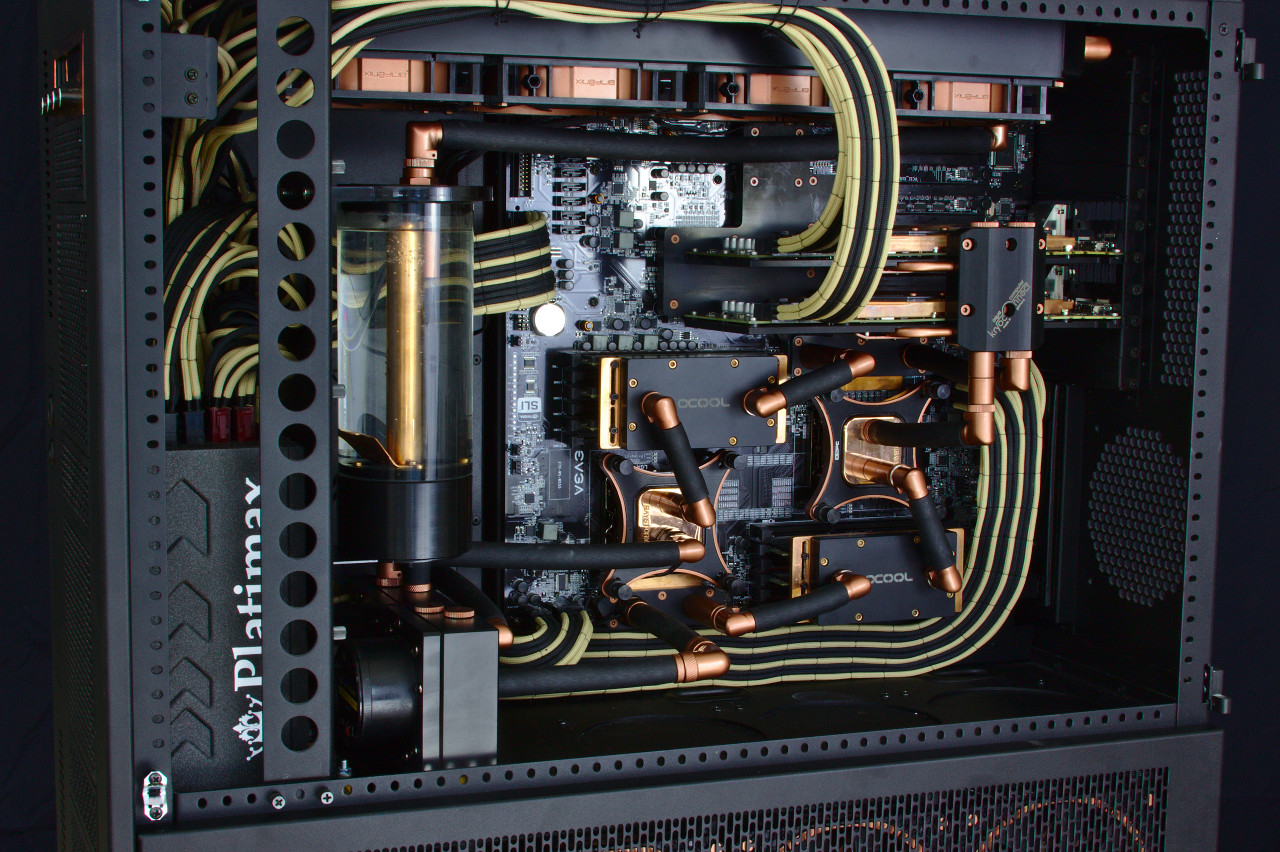
\includegraphics[width=120mm]{titlepic.jpg}

    \vfill

    \today\\
    Version 1.0.0
\end{titlingpage}
\frontmatter
\tableofcontents*

\mainmatter
\chapter{Text}
\lipsum[1]

\sffamily\lipsum[2]

\bfseries\lipsum[3]

\mdseries\ttfamily\lipsum[4]

\bfseries\ttfamily\lipsum[5]

\normalfont\scshape\lipsum[6]

\slshape\lipsum[7]

\scshape\lipsum[8]

\scslshape\lipsum[9]

\normalfont

\chapter{Tables}
\begin{table}
    \centering
    \caption{tabular inside float}
    \label{tab:float}
    \begin{tabular}{lll}
        \toprule
        \scshape Header 1 & \scshape Header 2 & \scshape Header 3 \\
        \midrule
        Content           & Content           & Content           \\
        Content           & Content           & Content           \\
        Content           & Content           & Content           \\
        Content           & Content           & Content           \\
        \bottomrule
    \end{tabular}
\end{table}

\lipsum[3]

\begin{center}
    \tabcaption{Tabular outside of float}
    \label{tab:outside}
    \begin{tabular}{lll}
        \toprule
        \scshape Header 1 & \scshape Header 2 & \scshape Header 3 \\
        \midrule
        Content           & Content           & Content           \\
        Content           & Content           & Content           \\
        Content           & Content           & Content           \\
        Content           & Content           & Content           \\
        \bottomrule
    \end{tabular}
\end{center}

\chapter{References and Hyperlinks}
This sentence refers to Table~\ref{tab:outside}.

This is a citation \cite{testitem}.

\href{https://hyperlink.com}{This is a hyperlink hiding behind text.}

\href{https://hyperlink.com}{\nolinkurl{https://hyperlink.com}}

\chapter{Sectional Headings}

This section illustrates the  style of \verb|\section|, \verb|\subsection| and
\verb|\subsubsection|.

\section{A Section}
\lipsum[2]

\subsection{A Subsection}
\lipsum[1]

\subsubsection{A subsubsection}
\lipsum[2]

\chapter{Code Listings}
\tikzset{external/export next=false}%
\begin{tcblisting}{%
        title=This Is a Code Listing,
        minted language=tex,
        listing side text,
        }
    \begin{tabular}{ll}
        a & a \\
        a & a \\
    \end{tabular}
\end{tcblisting}

\tikzset{external/export next=false}%
\begin{tcolorbox}[title=test]
    \lipsum[2]
\end{tcolorbox}

\tikzset{external/export next=false}%
\begin{tcolorbox}
    \lipsum[2]
\end{tcolorbox}

\chapter{Mathematics}

A numbered equation:
\begin{equation}
    y(x) = x^2 + 2x + 5
\end{equation}

An unnumbered equation:
\begin{equation*}
    x_{01,02} = -1 \pm 2j
\end{equation*}

An \verb|align| with some numbered and unnumbered lines:

\begin{align}
    \frac{\Phi}{i}
    & =
    \int_{0}^{\infty} \frac{dx}{x} \int_{0}^{l+m}
    \left[
        \frac{y dy}{\sqrt{x^2+y^2}} - \frac{(y-l) dy}{\sqrt{x^2+(y-l)^2}}
    \right]
    \nonumber
    \\
    &=
    \int_{0}^{\infty}
    \left[
        \sqrt{x^2 + (l+m)^2)} - \sqrt{x^2+l^2} - \sqrt{x^2+m^2}+x
    \right]
    \frac{dx}{x}
    \nonumber
    \\
    &=
    \Bigg[
        \sqrt{x^2 + (l+m)^2} - \sqrt{x^2+l^2} - \sqrt{x^2+m^2}
        \nonumber
        \\
        & ~~~~~~~~~   + x - l \cdot \log{\frac{l+m+\sqrt{x^2+(l+m)^2}}{l+\sqrt{x^2+l^2}}}
        \nonumber
        \\
        & ~~~~~~~~~   - m \cdot \log{\frac{l+m+\sqrt{x^2+(l+m)^2}}{m+\sqrt{x^2+l^2}}} ~
    \Bigg]_0^{\infty}
    \label{eq:mISL:2}
    \\
    & \approx
    \left[ l \cdot \log{\frac{l+m}{l}} + m \cdot \log{\frac{l+m}{m}} \right]
    \label{eq:mISL:3}
\end{align}


\cleardoublepage
\begin{titlingpage*}
    \fullhexpage{da2}{ct4}
    \begin{vplace}
        \flushright\Huge\bfseries\sffamily\appendixpagename
    \end{vplace}
\end{titlingpage*}
\appendix
\chapterstyle{alpenappendix}
\chapter{An Appendix Chapter}
\lipsum[1-3]

\chapter{Another Appendix Chapter with a Title That Requires Two Lines}
\lipsum[4-6]

\backmatter
\chapter{A Backmatter Chapter}
\lipsum[7-9]

\begin{thebibliography}{1}
    \bibitem{testitem}
        An Author, ``A Title``, 1979.
\end{thebibliography}
%% ============================================================== END CONTENT %
\end{document}
%</example>
% \fi
%^^A >>>
%
%^^A ------------------------------------------------------------------------- %
%^^A                                                  MULTI-LANGUAGE SUPPORT <<<
% \iffalse
%<*de>
\expandafter\newif\csname ifenglish\endcsname
\englishfalse
% \iffalse meta-comment
% -------------------------------------------------------- %
% Copyright (c) 2017 Raphael Frey rmfrey@runbox.com        %
% -------------------------------------------------------- %
%                                                          %
% This file  may be distributed and/or  modified under the %
% conditions of  the LaTeX Project Public  License, either %
% version 1.3c  of this  license or  (at your  option) any %
% later version. The latest version of this license is in: %
%                                                          %
%     http://www.latex-project.org/lppl.txt                %
%                                                          %
% and version 1.3c  or later is part  of all distributions %
% of LaTeX version 2008/05/04 or later.                    %
% -------------------------------------------------------- %
% \fi
%
%\CheckSum{0}
%
%
%^^A ------------------------------------------------------------------------- %
%^^A                                              DRIVER, PROVIDESCLASS ETC. <<<
% \iffalse
%<*driver>
\ProvidesFile{alpenthesis.dtx}
%</driver>
%<class>\NeedsTeXFormat{LaTeX2e}
%<class>\ProvidesClass{alpenthesis}%
%<*class>
    [2017/04/06 v0.0.1 PDF-LaTeX class for my thesis]
%</class>
%<*driver>
\expandafter\ifx\csname ifenglish\endcsname\relax
    \expandafter\newif\csname ifenglish\endcsname
    \englishtrue
\fi
\documentclass[a4paper,11pt,oneside]{ltxdoc}
\EnableCrossrefs
\CodelineIndex
\RecordChanges
% ----------------------------------------------- PACKAGES %
\usepackage[T1]{fontenc}
\usepackage[utf8]{inputenc}
\ifenglish
    \usepackage[english]{babel}
\else
    \usepackage[ngerman]{babel}
\fi
\usepackage{xcolor-solarized}
\usepackage[light,nott]{kpfonts}
\usepackage[scaled=0.8125]{DejaVuSansMono}
\usepackage{hypdoc}
\usepackage{tikz}
\usepackage{alpencolors}
\usepackage{booktabs}
\usepackage{imakeidx}
% ------------------------------------------ HELPER MACROS %
\newcommand*\pacname[1]{\textsf{#1}}
\newcommand*\code[1]{\texttt{#1}}
\newcommand*\athes{\pacname{alpenthesis}}
\newcommand*\memoir{\pacname{memoir}}
\begin{document} % ****************************** DOCUMENT %
    \DocInput{alpenthesis.dtx}
\end{document}
%</driver>
% \fi
%^^A >>>
%
%^^A ------------------------------------------------------------------------- %
%^^A                                                 GetFileInto, DoNotIndex <<<
% \GetFileInfo{alpenthesis.dtx}
% \DoNotIndex{\addtolength,\bfseries,\captiondelim,\captionnamefont}
% \DoNotIndex{\captiontitlefont,\checkandfixthelayout,\color,\Large}
% \DoNotIndex{\large,\LoadWithClassOptions,\maxsecnumdepth,\maxtocdepth}
% \DoNotIndex{\newcommand,\newfixedcaption,\pagestyle,\paperheight}
% \DoNotIndex{\paperwidth,\renewcommand,\RequirePackage,\setlength}
% \DoNotIndex{\setlrmarginsandblock,\setsecheadstyle,\setsubsecheadstyle}
% \DoNotIndex{\setsubsubsecheadstyle,\settrimmedsize,\settrims}
% \DoNotIndex{\setulmarginsandblock,\sffamily,\small,\stockaiii}
% \DoNotIndex{\stockwidth,\textsf,\texttt,\trimedge,\trimmarkscolor}
% \DoNotIndex{\trimtop}
% \DoNotIndex{\@chapapp,\addtodef,\afterchapskip,\afterchapternum}
% \DoNotIndex{\athes,\beforechapskip,\begin,\end}
% \DoNotIndex{\AT@bottomscreen,\chapnamefont,\chapnumfont}
% \DoNotIndex{\chapterheadstart,\chapternamenum,\chaptitlefont}
% \DoNotIndex{\edgewidth,\fadingIndex,\fi,\fill,\flushright,\foreach}
% \DoNotIndex{\globalcolorstrue,\height,\hspace,\HUGE,\includepdf}
% \DoNotIndex{\input,\iterstop,\iterstopvert,\j,\k,\LARGE,\leftTransp}
% \DoNotIndex{\MakeTextUppercase,\m,\makebox,\marginparsep,\marginparwidth}
% \DoNotIndex{\maxElementNumber,\midchapskip,\n,\newif,\newlength,\nobreak}
% \DoNotIndex{\numberOfHorizSides,\numberOfHorizElements,\offsetVert}
% \DoNotIndex{\par,\pgfkeysgetvalue,\pgfmathcos,\pgfmathmod,\pgfmathresult}
% \DoNotIndex{\pgfmathsetmacro,\pgfmathtruncatemacro,\pgfplotsset}
% \DoNotIndex{\printchaptername,\printchapternonum,\printchapternum}
% \DoNotIndex{\printchaptertitle,\x,\y,\resizebox}
% \DoNotIndex{\rightTransp,\rowtestcolor,\rule,\side,\spinemargin}
% \DoNotIndex{\textwidth,\thechapter,\thepage,\tikz,\tikzfading,\tikzset}
% \DoNotIndex{\usepackage,\usepgfplotslibrary,\usetikzlibrary,\vskip,\vspace}
%^^A>>>
%
%^^A ------------------------------------------------------------------------- %
%^^A                                                    TITLE, ABSTRACT, ToC <<<
% \author{Raphael Frey \\[1ex] \href{https://github.com/alpenwasser/}%
%                                     {\nolinkurl{https://github.com/alpenwasser/}}}
%
% \ifenglish
%   \title{The \athes\ Class\thanks{This document corresponds
%       to \athes~\fileversion, dated~\filedate.}}
%   \maketitle
%   \begin{abstract}
%        The \athes\  class is the  \LaTeX class I  wrote for my  thesis. It is
%        based on  the \memoir\  class and  is a  collection of  various custom
%        commands  and  configurations  to  suit my  personal  preferences  and
%        requirements. You may or  may not find some of it  useful, but keep in
%        mind that this is a class created  for a specific use case to cater to
%        a  select  few people's  preferences,  so  some  things may  not  seem
%        sensible or acceptable to you.
%
%        For  this  reason, the  class  does  not really  allow  for  a lot  of
%        customisation\footnotemark. It is primarily a ``fire-and-forget'' sort of affair.
%
%        \footnotetext{%
%            In principle,  most options and  commands from the  \memoir\ class
%            are present and  supported, but because this class loads  a lot of
%            packages  and preforms  a lot  of customization,  the results  may
%            sometimes  be undesired. I  have taken  no particular  precautions
%            when it comes to compatibility on  this level beyond what I needed
%            to make my personal configuration work as desired.}
%   \end{abstract}
% \else
%   \title{Die \athes-Klasse\thanks{Dieses Dokument entspricht
%          \athes~\fileversion, datiert~\filedate.}}
%   \maketitle
%   \begin{abstract}
%        Die \athes-Klasse  ist die \LaTeX-Klasse,  die ich f\"ur  meine Thesis
%        entwickelt habe,  aufbauend auf  der \memoir-Klasse. Sie  ist prim\"ar
%        eine Kollektion  von massgeschneiderten Befehlen  und Konfigurationen,
%        um   meine   pers\"onlichen   Bed\"urfnisse   und   Anforderungen   zu
%        erf\"ullen. Jemand  k\"onnte einen  Teil  davon allenfalls  n\"utzlich
%        finden. Man beachte  aber, dass diese Klasse  f\"ur einen spezifischen
%        Zweck f\"ur  einige wenige  Personen geschrieben  wurde. Somit m\"ogen
%        einige  Dinge  aus der  Sicht  der  geneigten Leserin  nicht  sinnvoll
%        implementiert sein.
%
%        Aus diesem  Grund ist  bei dieser  Klasse auch  nicht viel  Raum f\"ur
%        Konfiguration  vorgesehen\footnotemark. Es  ist  gr\"osstenteils  eine
%        ``fire-and-forget''-Angelegenheit.
%
%        \footnotetext{%
%            Im   Prinzip  werden   die  meisten   Optionen  und   Befehle  der
%            \pacname{memoir}-Klasse unterst\"utzt, aber  je nach Einstellungen
%            k\"onnten seltsame  Ergebnisse  auftreten,  da diese  Klasse viele
%            Packages l\"adt  und diverse Konfigurationen macht. Ich  habe hier
%            nicht explizit auf Kompatibilit\"at geachtet.}
%   \end{abstract}
% \fi
%
% \tableofcontents
%^^A >>>
%
%^^A ------------------------------------------------------------------------- %
%^^A                                                            INSTALLATION <<<
% \section{Installation}
% \label{sec:installation}
%
% \ifenglish
%    This section  deals with setting  up the \pacname{alpenthesis}  class and
%    setting up  a document with  it. Once you have generated  the \code{.cls}
%    class  file and  the \code{.pdf}  documentation (that  is: this  file, or
%    its  equivalent  in  another  language), or  have  received  those  files
%    from  somebody,  you  will   need  to  place  the  \code{alpenthesis.cls}
%    file  in  the  directory  of  your document  and  then  activate  it  via
%    |\documentclass{alpenthesis}|. See the \code{example.tex} for an example.
%
%    ^^A\inputminted[linenos=true,numbersep=4pt,fontsize=\footnotesize]{tex}{example.tex}
%   ^^A TODO: File structure tree with the needed files.
% \else
%    Dieser      Abschnitt      erkl\"art       die      Installation      der
%    \pacname{alpenthesis}-Klasse  und  erl\"autert,   wie  man  ein  Dokument
%    mit  ihr einrichtet. Nachdem  man  die \code{.cls}  Klassendatei und  die
%    Dokumentation  (dieses  Dokument,   oder  ein  anderssprachiges  Pendant)
%    generiert oder diese Dateien von  einer anderen Quelle erhalten hat, muss
%    man die Klassendatei \code{alpenthesis.cls} im selben Verzeichnis wie das
%    zu generierende Dokument platzieren und via |\documentclass{alpenthesis}|
%    aktivieren. Siehe  die  Datei   \code{example.tex},  welche  mitgeliefert
%    worden sein sollte.
% \fi
%^^A >>>
%
%^^A ------------------------------------------------------------------------- %
%^^A                                                          USER INTERFACE <<<
% \ifenglish
%    \section{User Interface}
%    \label{sec:user-interface}
% \else
%    \section{Benutzer-Interface}
%    \label{sec:user-interface}
% \fi
%
% |\documentclass\oarg{args}{alpenthesis}|\vspace{1em}
%
% \ifenglish
%    Loads  the  \athes\  class  with options  \meta{args}. Those  options  are
%    directly passed through to the  underlying \memoir\ class, so most options
%    for \memoir\  can be  specified. However, some may  be less  sensible than
%    others, given all the other configurations \athes\ makes.
%
%    If you require heavy customisation,  it is probably recommendable to start
%    off with the \memoir\ class itself as a base and build from there, relying
%    on its excellent documentation.
% \else
%    L\"adt    die    \athes-Klasse    mit    den    spezifizierten    Optionen
%    \meta{args}. Diese   Optionen   werden   direkt   an   die   unterliegende
%    \memoir-Klasse  weitergegeben. Somit  k\"onnen   beinahe  alle  f\"ur  die
%    \memoir-Klasse verf\"ugbaren Optionen  geladen werden. Man beachte jedoch,
%    dass  nicht unbedingt  alle  Optionen Sinn  machen,  da die  \athes-Klasse
%    selbst noch einige Konfigurationen vornimmt.
%
%    M\"ochte man  starke Individualisierungen  vornehmen, macht  es vermutlich
%    mehr Sinn, die  \memoir-Klasse direkt zu laden und  anhand der exzellenten
%    Dokumentation die gew\"unschte Konfiguration zu erstellen.
% \fi
% \DescribeMacro{\aiiistock}
% \DescribeMacro{\showtrimson}
% \DescribeMacro{\showtrimsoff}
% \ifenglish
%    Sets the  stock size to  A3 paper, keeping the  trimmed paper size  at A4,
%    vertically and  horizontally centered. Prints trim  marks for the  A4 page
%    centered on the A3 sheet.
%
%    To disable  trim marks,  you can  use the  |\showtrimsoff|. |\showtrimson|
%    will  enable them  again. Refer  to the  \memoir\  documentation for  more
%    information.
% \else
%    Setzt  die  Bogengr\"osse  auf  A3,  w\"ahrend  die  bedruckte  Seite  auf
%    A4  behalten wird.   Der  bedruckte Bereich  ist  vertikal und  horizontal
%    zentriert auf dem A3-Bogen. Druckt Markierungen um die A4-Seite.
%
%    Um  die  Markierungen zu  entfernen  kann  der |\showtrimsoff|-Befehl  von
%    \memoir\ benutzt werden. |\showtrimson| schaltet sie wieder ein. Siehe die
%    \memoir-Dokumentation.
% \fi
%
% \DescribeMacro{\hextrue}
% \DescribeMacro{\hexfalse}
% \ifenglish
%    In order to save time when compiling a document, the |\hexfalse| value can
%    be set in the preamble. This leads to the hexagon grind being omitted from
%    the chapter style.
%
%    Setting |\hextrue|  will enable the hexagons. This  lengthens compile time
%    significantly.
%
%    The principle is similar to the  |draft| option which is available in many
%    document classes and  packages. Personally I do not tend to  use that much
%    though because of  all the usual things which come  with |draft|, which is
%    why I decided to implement a separate command.
% \else
%    Um  Zeit  zu  sparen  beim   Kompilieren,  kann  man  |\hexfalse|  in  der
%    Pre\"aambel setzen. Dies f\"uhrt dazu,  dass die Hexagons im Kapitel-Style
%    nicht gedruckt werden.
%
%    Den  Wert   |\hextrue|  zu  setzen, aktiviert die  Hexagons. Dies
%    verl\"angert die Kompilierzeit bedeutend.
%
%    Das  Prinzip  ist  \"ahnlich  wie  die  in  vielen  Packages  und  Klassen
%    verf\"ugbare |draft|-Option. Da  ich diese  jedoch f\"ur  meinen Geschmack
%    im  Normalfall  etwas  viele  unerw\"unschte Seiteneffekte  hat,  ist  ein
%    unabh\"angiger Switch implementiert.
% \fi
%^^A >>>
%
% \StopEventually{\PrintIndex}
%^^A ------------------------------------------------------------------------- %
%^^A                                                          IMPLEMENTATION <<<
% \section{Implementation}
% \label{sec:implementation}
%
%^^A ---------------------------------------------- Loading the memoir Class <<<
% \ifenglish
%    \subsection{Loading the Base Class (\memoir)}
%    \label{subsec:memload}
%    The underlyng  class is  \memoir, and  all options  passed to  the \athes\
%    class are directly  passed on to \memoir\  via the |\LoadClassWithOptions|
%    command.
%
%    Additionally, the two hexagon configuration switches are defined.
% \else
%    \subsection{Laden der Basisklasse (\memoir)}
%    \label{subsec:memload}
%    Die  zugrundeliegende Klasse  ist \memoir. Alle  an \athes\  \"ubergebenen
%    Optionen   werden   direkt   an   die   \memoir-Klasse   \"ubergeben   via
%    |\LoadClassWithOptions|.
%
%    Im Weiteren werden  die beiden Konfigurations-Booloeans f\"ur die Hexagons
%    hier definiert.
% \fi
% \color{sqB}
%^^A Need the class guards to prevent the macro code from being included again
%^^A in example.tex and the German .tex file
% \iffalse
%<*class>
% \fi
%    \begin{macrocode}
\LoadClassWithOptions{memoir}
\newif\ifhex
\newif\ifpaper
%    \end{macrocode}
% \iffalse
%</class>
% \fi
% \color{black}
%^^A>>>
%^^A ---------------------------------------------- Fonts, inputenc, fontenc <<<
% \ifenglish
%    \subsection{General Configuration}
%    \label{subsec:general-config}
%    We choose  the \pacname{kpfonts}  Package for serif  and sans  serif fonts
%    with the  |light| option,  and \pacname{DejaVuSansMono} as  our typewriter
%    font. Also, we  ensure that we  can write our  source code files with UTF8
%    characters and have T1 font encoding for our output.
% \else
%    \subsection{Allgemeine Konfiguration}
%    \label{subsec:general-config}
%    Wir  w\"ahlen  \pacname{kpfonts} als  unsere  Schriftart  f\"ur Serif  und
%    Sans-Serif,  mit  der  |light|-Option,  und  \pacname{DejaVuSansMono}  als
%    unsere  Monospace-Schriftart. Wir  stellen   ebenfalls  sicher,  dass  wir
%    UTF8-Input in unserem  Quelltext haben k\"onnen und dass der  Output in T1
%    codiert wird.
% \fi
% \color{sqB}
% \iffalse
%<*class>
% \fi
%    \begin{macrocode}
\RequirePackage[rmx,nott,intlimits,sumlimits]{kpfonts}
\RequirePackage[scaled=0.8125]{DejaVuSansMono}
\RequirePackage[utf8]{inputenc}
\RequirePackage[T1]{fontenc}
%    \end{macrocode}
% \iffalse
%</class>
% \fi
% \color{black}
%^^A>>>
%^^A ------------------------------------------------ DOCUMENT COLOR PALETTE <<<
% \ifenglish
%    \subsection{Document Color Palette}
%    \label{subsec:colors}
%    We  define the  following  colors  as our  document  colors  in a  central
%    location.  This allows easy modification  of document colors while keeping
%    the entire document consistent.
% \else
%    \subsection{Farbpalette des Dokuments}
%    \label{subsec:colors}
%    Wir  definieren  die  folgenden  Farben  f\"ur  unser  Dokument  an  einer
%    zentralen Stelle.  Dies erlaubt es,  die Farbpalette des Dokuments einfach
%    zu  modifizieren  und  dabei  die   Farben  \"uber  das  gesamte  Dokument
%    konsistent zu behalten.
% \fi
% \color{sqB}
% \iffalse
%<*class|colors>
%^^A We  extract the  color information into  a package for  use in  the class
%^^A documentation.
%<colors>\ProvidesPackage{alpencolors}[2017/04/08 v1.0 color palette for alpenthesis]
% \fi
%    \begin{macrocode}
\RequirePackage{xcolor}
\globalcolorstrue
\newcommand*\testcolor[1]{\tikz \fill[#1] (0em,0ex) rectangle (2em,2ex);}
\newcommand*\rowtestcolor[1]{#1 & \tikz \fill[#1] (0em,0ex) rectangle (2em,2ex);}
%    \end{macrocode}
% \iffalse
%</class|colors>
% \fi
% \color{black}
% \ifenglish
%    \subsubsection{Dark-ish Colors}
%    \label{subsubsec:darkish}
% \else
%    \subsubsection{Eher Dunkle Farben}
%    \label{subsubsec:darkish}
% \fi
% \begin{center}
%     \small
%     \begin{tabular}{lllllllllll}
%         \toprule
%         \rowtestcolor{da0} &
%         \rowtestcolor{da1} &
%         \rowtestcolor{da2} &
%         \rowtestcolor{da3} &
%         \rowtestcolor{da4} \\
%         \bottomrule
%     \end{tabular}
% \end{center}
% \color{sqB}
% \iffalse
%<*class|colors>
% \fi
%    \begin{macrocode}
\definecolor{da0}{HTML}{002B36}  \definecolor{da1}{HTML}{073642}
\definecolor{da2}{HTML}{008080}  \definecolor{da3}{HTML}{800080}
\definecolor{da4}{HTML}{404040}
%    \end{macrocode}
% \iffalse
%</class|colors>
% \fi
% \color{black}
% \ifenglish
%    \subsubsection{Bright-ish Colors}
%    \label{subsubsec:brightish}
% \else
%    \subsubsection{Eher helle Farben}
%    \label{subsubsec:brightish}
% \fi
% \begin{center}
%     \small
%     \begin{tabular}{lllllllllll}
%         \toprule
%         \rowtestcolor{br0} &
%         \rowtestcolor{br1} &
%         \rowtestcolor{br2} \\
%         \bottomrule
%     \end{tabular}
% \end{center}
% \color{sqB}
% \iffalse
%<*class|colors>
% \fi
%    \begin{macrocode}
\definecolor{br0}{HTML}{BEB9AA}  \definecolor{br1}{HTML}{EEE8D5}
\definecolor{br2}{HTML}{FDF6E3}
%    \end{macrocode}
% \iffalse
%</class|colors>
% \fi
% \color{black}
% \ifenglish
%    \subsubsection{Contrast Color Palette}
%    \label{subsubsec:contrast}
% \else
%    \subsubsection{Kontrastfarben}
%    \label{subsubsec:contrast}
% \fi
% \begin{center}
%     \small
%     \begin{tabular}{lllllllllll}
%         \toprule
%         \rowtestcolor{ct0} &
%         \rowtestcolor{ct1} &
%         \rowtestcolor{ct2} &
%         \rowtestcolor{ct3} &
%         \rowtestcolor{ct4} \\
%         \rowtestcolor{ct5} &
%         \rowtestcolor{ct6} \\
%         \bottomrule
%     \end{tabular}
% \end{center}
% \color{sqB}
% \iffalse
%<*class|colors>
% \fi
%    \begin{macrocode}
\definecolor{ct0}{HTML}{CB4B16}  \definecolor{ct1}{HTML}{DC322F}
\definecolor{ct2}{HTML}{DC3682}  \definecolor{ct3}{HTML}{268BD2}
\definecolor{ct4}{HTML}{2AA198}  \definecolor{ct5}{HTML}{B58900}
\definecolor{ct6}{HTML}{859900}  \definecolor{sq0}{HTML}{F7FBFF}
%    \end{macrocode}
% \iffalse
%</class|colors>
% \fi
% \color{black}
% \ifenglish
%    \subsubsection{Sequential Color Palette}
%    \label{subsubsec:sequential}
% \else
%    \subsubsection{Sequentielle Farb-Palette}
%    \label{subsubsec:sequential}
% \fi
% \begin{center}
%     \small
%     \begin{tabular}{lllllllllll}
%         \toprule
%         \rowtestcolor{sq0} &
%         \rowtestcolor{sq1} &
%         \rowtestcolor{sq2} &
%         \rowtestcolor{sq3} &
%         \rowtestcolor{sq4} \\
%
%         \rowtestcolor{sq5} &
%         \rowtestcolor{sq6} &
%         \rowtestcolor{sq7} &
%         \rowtestcolor{sq8} &
%         \rowtestcolor{sq9} \\
%
%         \rowtestcolor{sqA} &
%         \rowtestcolor{sqB} &
%         \rowtestcolor{sqC} \\
%         \bottomrule
%     \end{tabular}
% \end{center}
% \color{sqB}
% \iffalse
%<*class|colors>
% \fi
%    \begin{macrocode}
\definecolor{sq1}{HTML}{EFF3FF}  \definecolor{sq2}{HTML}{DECDF7}
\definecolor{sq3}{HTML}{C6DBEF}  \definecolor{sq4}{HTML}{BDD7E7}
\definecolor{sq5}{HTML}{9ECAE1}  \definecolor{sq6}{HTML}{6BAED6}
\definecolor{sq7}{HTML}{4292C6}  \definecolor{sq8}{HTML}{3182BD}
\definecolor{sq9}{HTML}{2171B5}  \definecolor{sqA}{HTML}{08519C}
\definecolor{sqB}{HTML}{084594}  \definecolor{sqC}{HTML}{08306B}
%    \end{macrocode}
% \iffalse
%</class|colors>
% \fi
% \color{black}
% \ifenglish
%    \subsubsection{Divergent color palette}
%    \label{subsubsec:divergent}
% \else
%    \subsubsection{Divergierende Farb-Palette}
%    \label{subsubsec:divergent}
% \fi
% \begin{center}
%     \small
%     \begin{tabular}{lllllllllll}
%         \toprule
%         \rowtestcolor{dv-7} &
%         \rowtestcolor{dv-6} &
%         \rowtestcolor{dv-5} &
%         \rowtestcolor{dv-4} &
%         \rowtestcolor{dv-3} \\
%
%         \rowtestcolor{dv-2} &
%         \rowtestcolor{dv-1} &
%         \rowtestcolor{dv+0} &
%         \rowtestcolor{dv+1} &
%         \rowtestcolor{dv+2} \\
%
%         \rowtestcolor{dv+3} &
%         \rowtestcolor{dv+4} &
%         \rowtestcolor{dv+5} &
%         \rowtestcolor{dv+6} &
%         \rowtestcolor{dv+7} \\
%         \bottomrule
%     \end{tabular}
% \end{center}
% \color{sqB}
% \iffalse
%<*class|colors>
% \fi
%    \begin{macrocode}
\definecolor{dv-7}{HTML}{8E0152} \definecolor{dv-6}{HTML}{C51B7D}
\definecolor{dv-5}{HTML}{D01C8B} \definecolor{dv-4}{HTML}{DE77AE}
\definecolor{dv-3}{HTML}{E9A3C9} \definecolor{dv-2}{HTML}{F1B6DA}
\definecolor{dv-1}{HTML}{FDE0EF} \definecolor{dv+0}{HTML}{F7F7F7}
\definecolor{dv+1}{HTML}{D1E5F0} \definecolor{dv+2}{HTML}{92C5DE}
\definecolor{dv+3}{HTML}{67A9CF} \definecolor{dv+4}{HTML}{4393C3}
\definecolor{dv+5}{HTML}{0571B0} \definecolor{dv+6}{HTML}{2166AC}
\definecolor{dv+7}{HTML}{053061}
%    \end{macrocode}
% \iffalse
%</class|colors>
% \fi
% \color{black}
% \ifenglish
%    \subsubsection{Qualitative Color Palette}
%    \label{subsubsec:qualitative}
% \else
%    \subsubsection{Qualitative Farb-Palette}
%    \label{subsubsec:qualitative}
% \fi
% \begin{center}
%     \small
%     \begin{tabular}{lllllllllll}
%         \toprule
%         \rowtestcolor{q0} &
%         \rowtestcolor{q1} &
%         \rowtestcolor{q2} &
%         \rowtestcolor{q3} &
%         \rowtestcolor{q4} \\
%
%         \rowtestcolor{q5} &
%         \rowtestcolor{q6} &
%         \rowtestcolor{q7} \\
%         \bottomrule
%     \end{tabular}
% \end{center}
% \color{sqB}
% \iffalse
%<*class|colors>
% \fi
%    \begin{macrocode}
\definecolor{q0}{named}{ct3}   \definecolor{q1}{named}{sqB}
\definecolor{q2}{named}{ct2}   \definecolor{q3}{named}{da3}
\definecolor{q4}{HTML}{FEC44F} \definecolor{q5}{named}{ct0}
\definecolor{q6}{HTML}{80EA82} \definecolor{q7}{HTML}{2E7D32}
%    \end{macrocode}
% \iffalse
%</class|colors>
% \fi
% \color{black}
%^^A NOTE: each \rowtestcolor command requires two columns!
%^^A >>>
%^^A --------------------------------------------------- TikZ, PGF, PGFPLOTS <<<
% \ifenglish
%    \subsection{Ti\emph{k}Z, \textsc{pgfplots}}
%    \label{subsec:tikz-pgfplots}
% \else
%    \subsection{Ti\emph{k}Z, \textsc{pgfplots}}
%    \label{subsec:tikz-pgfplots}
% \fi
% \color{sqB}
% \iffalse
%<*class>
% \fi
%    \begin{macrocode}
\RequirePackage{tikz}
\usetikzlibrary{calc}
\usetikzlibrary{fadings}
\RequirePackage{pgfplots}
\pgfplotsset{compat=1.14}
\usepgfplotslibrary{external}
\tikzexternalize[prefix=cache/,optimize command away=\includepdf]
%    \end{macrocode}
% \iffalse
%</class>
% \fi
% \color{black}
%^^A >>>
%^^A -------------------------------------------------- HEXAGON CALCULATIONS <<<
% \ifenglish
%    \subsection{Hexagon Calculations}
%    \label{subsec:hexagon-calcs}
%    In this section,  the various required calculations for  the hexagon grids
%    are made. The basis is the number  of hexagons sides (not hexagons!) which
%    are to fit into one page width. Going  from there, the height of a hexagon
%    as well as the number of rows and columns are calculated.
% \else
%    \subsection{Berechnungen f\"ur Hexagons}
%    \label{subsec:hexagon-calcs}
%    An  dieser   Stelle  werden   diverse  Berechnungen  f\"ur   die  Hexagons
%    ausgef\"uhrt.  Grundlage ist die  Anzahl Hexagon-Seitenl\"angen (nicht die
%    Anzahl  Hexagons!), welche  in eine  Seitenbreite passt. Darauf  basierend
%    werden die halbe H\"ohe eines Hexagons sowie die Anzahl Spalten und Zeilen
%    berechnet.
% \fi
% \color{sqB}
% \iffalse
%<*class>
% \fi
%    \begin{macrocode}
\pgfmathsetmacro\AT@paperwidth{21}
\pgfmathsetmacro\AT@paperheight{29.7}
\pgfmathsetmacro\AT@numberOfSidesHorizontally{22}
\pgfmathsetmacro\AT@side
    {\AT@paperwidth / \AT@numberOfSidesHorizontally}
\pgfmathtruncatemacro\AT@totCols
    {0.666667 * \AT@numberOfSidesHorizontally + 1}
\pgfmathcos{30}
\pgfmathsetmacro\AT@height
    {\pgfmathresult * \AT@side}
\pgfmathtruncatemacro\AT@numberOfHeightsVertically
    {\AT@paperheight / \AT@height}
\pgfmathtruncatemacro\AT@totRows
    {0.5 * \AT@numberOfHeightsVertically + 1}
\pgfmathtruncatemacro\AT@totRowsChap
    {0.1333 * \AT@numberOfHeightsVertically + 1}
%    \end{macrocode}
% \iffalse
%</class>
% \fi
% \color{black}
% \ifenglish
%    If the print version is to be generated, a uniform color for each hexagon,
%    depending on its horizontal and vertical position, is calculated:
% \else
%    Falls  die Druckversion  erstellt werden  soll, wird  eine uniforme  Farbe
%    f\"ur  jedes Hexagon,  abh\"angig von  seiner horizontalen  und vertikalen
%    Position, generiert:
% \fi
% \color{sqB}
% \iffalse
%<*class>
% \fi
%    \begin{macrocode}
\AtBeginDocument{%
    \ifpaper
        \foreach \y in {0,...,\AT@totRowsChap} {%
            \foreach \x in {0,...,\AT@totCols}{%
                \pgfmathsetmacro\mix
                    {100 * \x / \AT@totCols}%
                \pgfmathsetmacro\mixvert
                    {100 * \y / \AT@totRowsChap}%
                \colorlet{hex-\x}{white!\mix!br0}%
                \colorlet{hex-\x-\y}{white!\mixvert!hex-\x}%
                \colorlet{hexframecol-\x}{white!\mix!br2}%
                \colorlet{hexframecol-\x-\y}
                    {white!\mixvert!hexframecol-\x}%
                \colorlet{chapcol-\x}{dv-4!\mix!dv-7}%
                \colorlet{chapcol-\x-\y}
                    {dv-2!\mixvert!chapcol-\x}%
                \colorlet{appcol-\x}{ct4!\mix!da2}%
                \colorlet{appcol-\x-\y}{white!\mixvert!appcol-\x}%
            }%
        }%
%    \end{macrocode}
% \iffalse
%</class>
% \fi
% \color{black}
% \ifenglish
%    For the  electronic version,  fadings are used  instead. Unfortunately, we
%    cannot simply have one global fading  which applies to all hexagons (since
%    each hexagon is  a single path)\footnotemark, so one  fading is calculated
%    for each  hexagon based  on its  horizontal position. The  vertical fading
%    effect is later achieved by  overlaying a white-to-transparent screen from
%    the grid's bottom edge. Maybe one day I'll figure out how to combine these
%    into one single and nice step.
%
%    \footnotetext{%
%        Or more accurately: I  have not been able to find  a way to accomplish
%        this.}
% \else
%    F\"ur die elektronische Version werden stattdessen Fadings benutzt. Leider
%    kann  nicht  einfach   ein  globales  Fading  definiert   und  \"uber  das
%    gesamte  Gitter  gelegt  werden  (da   jedes  einzelne  Hexagon  ein  Pfad
%    ist)\footnotemark, deshalb  wird f\"ur jedes Hexagon  ein Fading bestimmt,
%    abh\"angig  von   der  horizontalen  Position  im   Gitter. Der  vertikale
%    Fading-Effekt  wird  mit   einem  weiss-zu-transparenten  Fading  erzeugt,
%    welches dem gesamten Gitter  von unten \"uberlagert wird. Vielleicht finde
%    ich  eines  Tages eine  clevere  Variante,  die  beiden Effekte  in  einen
%    einzelnen, eleganten Schritt zu kombinieren.
%
%    \footnotetext{%
%        Oder genauer  gesagt: Ich habe  bisher nicht herausgefunden,  wie dies
%        m\"oglich w\"are.}
% \fi
% \color{sqB}
% \iffalse
%<*class>
% \fi
%    \begin{macrocode}
    \else
        \foreach \x in {0,...,\AT@totCols}{%
            \pgfmathsetmacro\leftTransp
                {100 *  \x    / \AT@totCols}%
            \pgfmathsetmacro\rightTransp
                {100 * (\x+1) / \AT@totCols}%
            \tikzfading[%
                name=hexfade \x,
                right color=transparent!\rightTransp,
                left color=transparent!\leftTransp]%
        }%
    \fi
}
\newcommand\AT@providehexagonpath[3]{%
    ($(current page.north west) +
        (1.5 * #1 * \AT@side,
            #3 * \AT@height - #2 * 2 * \AT@height)$)
    -- ++(   0:\AT@side)
    -- ++( -60:\AT@side)
    -- ++(-120:\AT@side)
    -- ++(-180:\AT@side)
    -- ++(-240:\AT@side) -- cycle;
}
%    \end{macrocode}
% \iffalse
%</class>
% \fi
% \color{black}
%^^A >>>
%^^A ------------------------------------------ HEXAGON FULL PAGE BACKGROUND <<<
% \ifenglish
%    \subsection{Hexagon Page Background}
%    \label{subsec:hexagon-background}
% \else
%    \subsection{Hexagon Seitenhintergrund}
%    \label{subsec:hexagon-background}
% \fi
% \color{sqB}
% \iffalse
%<*class>
% \fi
%    \begin{macrocode}
\newcommand\fullhexpage[2]{%
    \ifhex
        \tikzset{external/export next=false}%
        \begin{tikzpicture}[remember picture,overlay,x=1cm,y=1cm]
            \path[clip]
                (current page.north west)
                rectangle
                (current page.south east);
            \foreach \y in {0,...,\AT@totRows} {%
                \foreach \x in {0,...,\AT@totCols} {%
                    \pgfmathsetmacro\AT@isodd{mod(\x,2)}
                    \fill[fill=br2,draw=br1]
                        \AT@providehexagonpath{\x}{\y}{\AT@isodd}
                }
            }
            % Create vertical contrast bar on left side.
            % Put it inside scope for clipping.
            \begin{scope}
                \path[clip]
                    (current page.north west)
                    rectangle
                    ($(current page.south west) +
                        (3.5 * \AT@side,0)$);
                \foreach \y in {0,...,\AT@totRows} {%
                    \foreach \x in {0,...,2} {%
                        \pgfmathsetmacro\AT@isodd{mod(\x,2)}
                        \fill[fill=#1,draw=#2]
                            \AT@providehexagonpath{\x}{\y}{\AT@isodd}
                    }
                }
            \end{scope}
        \end{tikzpicture}%
    \fi
}
%    \end{macrocode}
% \iffalse
%</class>
% \fi
% \color{black}
%^^A>>>
%^^A ------------------------------------------------------------- tcolorbox <<<
% \ifenglish
%    \subsection{\pacname{tcolorbox}}
%    \label{subsec:tcolorbox}
%
%    Keeping with the theme of angled things, we define an octagon shape
%    as the surrounding shape for \pacname{tcolorbox}.
% \else
%    \subsection{\pacname{tcolorbox}}
%    \label{subsec:tcolorbox}
%
%    Um zum allgemeinen Thema der gewinkelten Dinge zu passen, wird ein Oktagon
%    als Form f\"ur den Rahmen der \pacname{tcolorbox}-Elemente definiert.
% \fi
% \color{sqB}
% \iffalse
%<*class>
% \fi
%    \begin{macrocode}
\RequirePackage{tcolorbox}
\tcbuselibrary{minted}
\tcbuselibrary{skins}
\tcbset{%
    colback=br2,
    coltitle=br2,
    colframe=da1,
    fonttitle=\sffamily,
    minted options={autogobble},
    enhanced,
    frame code={
        \draw[very thick]
               ([xshift=-3mm,yshift=+1mm]frame.north east)
            -- ([xshift=+0mm,yshift=-2mm]frame.north east)
            -- ([xshift=+0mm,yshift=+2mm]frame.south east)
            -- ([xshift=-3mm,yshift=-1mm]frame.south east)
            -- ([xshift=+3mm,yshift=-1mm]frame.south west)
            -- ([xshift=-0mm,yshift=+2mm]frame.south west)
            -- ([xshift=-0mm,yshift=-2mm]frame.north west)
            -- ([xshift=+3mm,yshift=+1mm]frame.north west)
            -- cycle;
    },
    interior titled code={%
        \path[tcb fill interior]
               ([xshift=-2.7mm,yshift=+1.3mm]interior.north east)
            -- ([xshift=+0.3mm,yshift=-1.7mm]interior.north east)
            -- ([xshift=+0.3mm,yshift=+1.7mm]interior.south east)
            -- ([xshift=-2.7mm,yshift=-1.3mm]interior.south east)
            -- ([xshift=+2.7mm,yshift=-1.3mm]interior.south west)
            -- ([xshift=-0.3mm,yshift=+1.7mm]interior.south west)
            -- ([xshift=-0.3mm,yshift=-1.7mm]interior.north west)
            -- ([xshift=+2.7mm,yshift=+1.3mm]interior.north west)
            -- cycle;
    },
    interior code={%
        \path[tcb fill interior]
               ([xshift=-2.7mm,yshift=+1.3mm]interior.north east)
            -- ([xshift=+0.3mm,yshift=-1.7mm]interior.north east)
            -- ([xshift=+0.3mm,yshift=+1.7mm]interior.south east)
            -- ([xshift=-2.7mm,yshift=-1.3mm]interior.south east)
            -- ([xshift=+2.7mm,yshift=-1.3mm]interior.south west)
            -- ([xshift=-0.3mm,yshift=+1.7mm]interior.south west)
            -- ([xshift=-0.3mm,yshift=-1.7mm]interior.north west)
            -- ([xshift=+2.7mm,yshift=+1.3mm]interior.north west)
            -- cycle;
    },
    title code={%
        \path[tcb fill frame]
               ([xshift=-3mm,yshift=+1mm]frame.north east)
            -- ([xshift=+0mm,yshift=-2mm]frame.north east)
            -- ([xshift=+0.3mm,yshift=-2mm]interior.north east)
            -- ([xshift=-3mm,yshift=+1mm]interior.north east)
            -- ([xshift=+3mm,yshift=+1mm]interior.north west)
            -- ([xshift=-0.3mm,yshift=-2mm]interior.north west)
            -- ([xshift=-0mm,yshift=-2mm]frame.north west)
            -- ([xshift=+3mm,yshift=+1mm]frame.north west)
            -- cycle;
    }
}
%    \end{macrocode}
% \iffalse
%</class>
% \fi
% \color{black}
%^^A >>>
%^^A ------------------------------------ OTHER PACKAGES WOTHOUT MUCH CONFIG <<<
% \ifenglish
%    \subsection{Other Packages}
%    \label{subsec:other-packages}
% \else
%    \subsection{Andere Packages}
%    \label{subsec:other-packages}
% \fi
% \color{sqB}
% \iffalse
%<*class>
% \fi
%    \begin{macrocode}
\RequirePackage[%
    pdfauthor=alpenwasser,
    pdfsubject={LaTeX document design},
    pdftitle={alpenwasser's thesis},
    bookmarksnumbered=true,
    pdfkeywords={LaTeX,design,alpenwasser,thesis,class,hexagons},
    colorlinks=true,
    linkcolor=sqB,
    citecolor=ct4,
    urlcolor=dv-6]{hyperref}
\RequirePackage[english]{babel}
\RequirePackage{amsmath}
\RequirePackage[separate-uncertainty=true]{siunitx}
\RequirePackage{counttexruns}
%    \end{macrocode}
% \iffalse
%</class>
% \fi
% \color{black}
%^^A >>>
%^^A --------------------------------------------------------- MEMOIR CONFIG <<<
%
%^^A -------------------------------------------------------- General Config <<<
% \ifenglish
%   \subsection{\memoir\ Configuration}
%   \label{subsec:memconfig}
%   \subsubsection{General Configuration}
%   \label{subsubsec:memoir:general-config}
% \else
%   \subsection{\memoir-Konfiguration}
%   \label{subsec:memconfig}
%   \subsubsection{Allgemeine Konfiguration}
%   \label{subsubsec:memoir:general-config}
% \fi
% \color{sqB}
% \iffalse
%<*class>
% \fi
%    \begin{macrocode}
\maxsecnumdepth{subsubsection}
\maxtocdepth{subsubsection}
\chapterstyle{veelo}
%    \end{macrocode}
% \iffalse
%</class>
% \fi
% \color{black}
%^^A>>>
%^^A ----------------------------------------------------------- Page Layout <<<
% \ifenglish
%     \subsubsection{Page Layout}
%     \label{subsubsec:page-layout}
% \else
%     \subsubsection{Seiten-Layout}
%     \label{subsubsec:page-layout}
% \fi
% \color{sqB}
% \iffalse
%<*class>
% \fi
%    \begin{macrocode}
\newcommand\aiiistock{%
    \stockaiii
    \settrimmedsize{297mm}{210mm}{*}
    \setlength{\trimtop}{\stockheight}
    \addtolength{\trimtop}{-\paperheight}
    \setlength{\trimedge}{\stockwidth}
    \addtolength{\trimedge}{-\paperwidth}
    \settrims{0.5\trimtop}{0.5\trimedge}
    \renewcommand*{\trimmarkscolor}{\color{red}}
    \showtrimson
    \checkandfixthelayout
}
\showtrimsoff
\setlrmarginsandblock{0.142857111\paperwidth}{0.190476190\paperwidth}{*}
\setulmarginsandblock{0.111111111\paperheight}{*}{1.5}%
\checkandfixthelayout
%    \end{macrocode}
% \iffalse
%</class>
% \fi
% \color{black}
%^^A>>>
%^^A -------------------------------------------- Sectional Title Formatting <<<
% \ifenglish
%    \subsubsection{Sectional Title Fonts and Styles} ^^A ---- Sec Title Fonts %
%    \label{subsubsec:title-fonts}
%    Sets font styles and other stylistic attributes for headings.
% \else
%    \subsubsection{Schriftarten und Stil f\"ur Titel von Abschnitten}
%    \label{subsubsec:title-fonts}
%    Definiert Schriftarten und andere Stil-Attribute f\"ur \"Uberschriften.
% \fi
% \color{sqB}
% \iffalse
%<*class>
% \fi
%    \begin{macrocode}
\setsecheadstyle{\color{sqB}\Large\bfseries\sffamily}
\setsubsecheadstyle{\color{sqB}\large\bfseries\sffamily}
\setsubsubsecheadstyle{\color{sqB}\bfseries\sffamily}
\addtodef{\printchaptername}{\color{sqB}}{}
%    \end{macrocode}
% \iffalse
%</class>
% \fi
% \color{black}
%^^A>>>
%^^A --------------------------------------------------- Headers and Footers <<<
% \ifenglish
%   \subsubsection{Headers and Footers}
%   \label{subsubsec:headers-footers}
% \else
%   \subsubsection{Kopf- und Fusszeilen}
%   \label{subsubsec:headers-footers}
% \fi
% \color{sqB}
% \iffalse
%<*class>
% \fi
%    \begin{macrocode}
\pagestyle{headings}
%    \end{macrocode}
% \iffalse
%</class>
% \fi
% \color{black}
%^^A>>>
%^^A -------------------------------------------------------------- Captions <<<
% \ifenglish
%   \subsubsection{Captions}
%   \label{subsubsec:captions}
% \else
%   \subsubsection{Legenden}
%   \label{subsubsec:captions}
% \fi
% \color{sqB}
% \iffalse
%<*class>
% \fi
%    \begin{macrocode}
\captionnamefont{\bfseries\small}
\captiontitlefont{\small}
\captiondelim{: }
% Captions for use outside of floats
\newfixedcaption{\figcaption}{figure}
\newfixedcaption{\tabcaption}{table}
%    \end{macrocode}
% \iffalse
%</class>
% \fi
% \color{black}
%^^A>>>
%^^A -------------------------------------------------------- Chapter Styles <<<
% \color{black}
% \ifenglish
%   \subsubsection{Chapter Style}
%   \label{subsubsec:chapterstyle}
%    The chapters are styled with grid of hexagons whose color is faded towards
%    the right sight of the page and towards the bottom. There are two versions
%    of  this  mechanisms: One for  printing,  activated  via the  |\papertrue|
%    switch, and  one for  the electronic document  version, activated  via the
%    |\paperfalse| switch (or no switch at all).
%
%    The  reason for  the two  implementation is  that the  electronic  version
%    uses  fadings  and   transparency,  which  can  cause   issues  with  some
%    printers\footnotemark.  Therefore,  instead of fadings, the  print version
%    uses  hexagons which  have slightly  differing colors, but each  hexagon's
%    color is  uniform. This does  not look  quite as nice  on the  screen, but
%    printing results have been satisfactory for  me so far, though obviously I
%    would prefer the faded version to just work. Your mileage may vary.
%
%    \footnotetext{%
%        I have had a  Canon printer do a hard reset while  trying to print the
%        faded version from a USB  stick plugged into the  printer. Our Kyocera
%        printer simply  printed a black bar  instead of hexagons when  I tried
%        doing the same.}
%
%    The  |\AT@hexagons|  command prints  the  background  hexagon grid  for
%    numbered chapters, appendix chapters and unnumbered chapters.
% \else
%   \subsubsection{Kapitel-Stil}
%   \label{subsubsec:chapterstyle}
%    Die  Kapitel  werden  mit  einem  Gitter  von  Hexagons  dekoriert,  deren
%    Farbe  gegen rechts  und gegen  unten  verblasst in  Richtung weiss  (bzw.
%    transparent). Es gibt  zwei Verianten  dieses Mechanismus: Eine  f\"ur die
%    elektronische  Version,  welche  die   Standardeinstellung  ist  oder  mit
%    |\paperfalse| explizit aktiviert  werden kann, und eine  Version f\"ur den
%    Druck, welche mit |\papertrue| aktiviert wird.
%
%    Der  Grund   f\"ur  die   zwei  unterschiedlichen   Implementationen  ist,
%    dass   Drucker    h\"aufig   Probleme   mit   Transparenz    und   Fadings
%    haben\footnotemark. Die   Druckversion   benutzt   daher   statt   Fadings
%    unterschiedliche  Farben f\"ur  die Hexagons,  wobei jedoch  jedes Hexagon
%    eine  uniforme Farbe  hat. Dies  sieht  nicht ganz  so  nett  aus auf  dem
%    Bildschirm,  aber  Druckresultate  waren   bisher  ganz  gut,  obwohl  ich
%    es  nat\"urlich  bevorzugen  w\"urde,  wenn  die  Fading-Variante  einfach
%    funktionieren w\"urde. Your mileage may vary.
%
%    \footnotetext{%
%        Ich habe  bei einem Canon-Drucker  erlebt, dass er einen  harten Reset
%        machte,  als ich  versuchte, das  Dokument mit  Transparenz von  einem
%        USB-Stick  zu drucken,  der direkt  am Drucker  eingesteckt war. Unser
%        Kyocera-Drucker  druckte  statt  der   Hexagons  einach  einen  dicken
%        schwarzen Balken beim selben Versuch.}
%
%    Der  |\AT@hexagons|-Befehl druckt  das  Hintergrundgitter mit  Hexagons
%    f\"ur numerierte und unnumerierte Kapitel sowie Kapitel im Appendix.
% \fi
% \color{sqB}
% \iffalse
%<*class>
% \fi
%    \begin{macrocode}
\newcommand\AT@hexagons{%
    \tikzset{external/export next=false}%
    \begin{tikzpicture}[remember picture,overlay,x=1cm,y=1cm]
%    \end{macrocode}
% \iffalse
%</class>
% \fi
% \color{black}
% \ifenglish
%    Remove anything that is outside the page.
% \else
%    Allen Inhalt entfernen, der ausserhalb der Seite liegt.
% \fi
% \color{sqB}
% \iffalse
%<*class>
% \fi
%    \begin{macrocode}
        \ifpaper
            \path[clip]
                (current page.north west)
                rectangle
                ($(current page.north east) + (-0pt,-11 * \AT@height)$);
        \else
            \path[clip]
                (current page.north west)
                rectangle
                ($(current page.north east) + (-0pt,-11 * \AT@height)$);
        \fi
%    \end{macrocode}
% \iffalse
%</class>
% \fi
% \color{black}
% \ifenglish
%    The outer loop iterates over the  rows, while the inner loop iterates over
%    the columns. Because the hexagons are offset by one |\AT@height| in the
%    vertical direction between  even and odd columns, we must  for each column
%    determine if it is an even or odd one, and then offset it, or not.
%
%    Also,  depending   on  whether   we're  in   |\papertrue|  mode   or  not,
%    we   either  use   the   fadings   or  uniform   colors   as  defined   in
%    Section~\ref{subsec:hexagon-calcs}.
% \else
%    Die  \"aussere   Schleife  iteriert  \"uber  die   Zeilen,  w\"ahrend  die
%    innere Schleife  \"uber die  Spalten iteriert. Weil  die Hexagons  um eine
%    |\@AT@height| versetzt sind, abh\"angig davon,  ob sie in einer geraden
%    oder ungeraden Spalte sind, muss f\"ur jede Spalte bestimmt werden, ob sie
%    gerade oder ungerade ist, um sie dann entsprechend zu versetzen, oder eben
%    nicht.
%
%    Im  Weiteren  werden,  abh\"angig   davon  ob  wir  im  |\papertrue|-Modus
%    sind oder  nicht, die in  Abschnitt~\ref{subsec:hexagon-calcs} definierten
%    Fadings oder Farben benutzt.
% \fi
% \color{sqB}
% \iffalse
%<*class>
% \fi
%    \begin{macrocode}
        \foreach \y in {0,...,\AT@totRowsChap} {%
            \foreach \x in {0,...,\AT@totCols} {%
                \pgfmathsetmacro\AT@isodd{mod(\x,2)}
                \ifpaper
                    \path[fill=hex-\x-\y,draw=hexframecol-\x-\y]
                \else
                    \path[fill=br0,draw=br1,path fading=hexfade \x]
                \fi
                    \AT@providehexagonpath{\x}{\y}{\AT@isodd}
            }%
        }%
    \end{tikzpicture}%
}
%    \end{macrocode}
% \iffalse
%</class>
% \fi
% \color{black}
%
% \DescribeMacro{\AT@numhexagons}%
% \ifenglish
%    The |\AT@numhexagons| command prints a number of hexagon colored in
%    a  contrast  color. The number  of  hexagons  corresponds to  the  current
%    chapter  number. This command  is  therefore not  executed for  unnumbered
%    chapters.
%
%    The  mechanism for  the offset  based  on even  or odd  column numbers  is
%    identical to the one used in the background hexagon grid.
%
%    The command requires four arguments:\newline\color{sqB}
%    |\AT@numhexagons|\marg{1,A}\marg{chapter,appendix}\marg{appcol,chapcol}\marg{color}
%    \color{black}
%    The  syntax  \meta{X,Y} indicates  that  either  \emph{X} or  \emph{Y}  is
%    required.
%    \begin{description}
%        \item[\normalfont\color{sqB}\meta{1,A}:] The  starting  point for  the
%            iteration  of  the  chapter  number. |1|  for  regularly  numbered
%            chapters,  |A| for  appendix chapters. Must  be one  of these  two
%            choices.
%
%        \item[\normalfont\color{sqB}\meta{chapter,appendix}:] Is used  to look
%            up the randomly  generated coordinates in the PGF key  trey in the
%            |randInts.tex| file. Must be one of these two choices.
%
%        \item[\normalfont\color{sqB}\meta{appcol,chapcol}:] The  color  prefix
%            string for  appendix and numbered chapters,  respectively, for the
%            paper version. Must be one of these two choices.
%
%        \item[\normalfont\color{sqB}\meta{color}:] The  color which  is to  be
%            used to fill  the contrast hexagons in the case  of the electronic
%            version. Can be any defined color.
%    \end{description}
% \else
%    Der  |\AT@numhexagons|-Befehl druckt  Hexagons in  einer Kontrastfarbe,
%    deren  Anzahl der  aktuellen Kapitelnummer  entspricht. F\"ur unnumerierte
%    Kapitel wird dieser Befehl nat\"urlich nicht ausgef\"uhrt.
%
%    Der  Mechanismus  zur Bestimmung  der  Versetzung  abh\"angig von  gerader
%    respektive ungerader  Spalten-Nummer ist identisch zu  demjenigen, welcher
%    f\"ur das Hintergrund-Grid verwendet wird.
%
%    Der Befehl ben\"otigt vier  Parameter:\newline\color{sqB}
%    |\AT@numhexagons|\marg{1,A}\marg{chapter,appendix}\marg{appcol,chapcol}\marg{color}
%    \color{black}
%    Die Syntax  \meta{X,Y} signalisiert, dass entweder  \emph{X} oder \emph{Y}
%    angegeben werden muss.
%    \begin{description}
%        \item[\normalfont\color{sqB}\meta{1,A}:] Der   Startpunkt  f\"ur   die
%            Iteration der Kapitelzahl.  |1|  f\"ur normal nummerierte Kapitel,
%            |A| f\"ur  Kapitel im Anhang.   Muss eine dieser  beiden Varianten
%            sein.
%
%        \item[\normalfont\color{sqB}\meta{chapter,appendix}:] Wird benutzt, um
%            im PGF-Baum in der Datei |randInts.tex| die zuf\"allig generierten
%            Koordinaten f\"ur das jeweils  aktive Hexagon nachzuschauen.  Muss
%            eine dieser beiden Varianten sein.
%
%        \item[\normalfont\color{sqB}\meta{appcol,chapcol}:] Das   Prefix   der
%            Kontrastfarbe f\"ur  nummerierte Kapitel bzw. Kapitel  des Anhangs
%            im  Falle der  Papierversion.  Muss  eine dieser  beiden Varianten
%            sein.
%
%        \item[\normalfont\color{sqB}\meta{color}:] Kontrastfarbe    bei    der
%            elektronischen Version. Kann eine beliebige g\"ultige Farbe sein.
%    \end{description}
% \fi
% \color{sqB}
% \iffalse
%<*class>
% \fi
%    \begin{macrocode}
\newcommand\AT@numhexagons[4]{%
    \tikzset{external/export next=false}%
    \begin{tikzpicture}[remember picture,overlay,x=1cm,y=1cm]
        \path[clip]
            (current page.north west) rectangle (current page.east);
        \foreach \n in {#1,...,\thechapter} {%
            \pgfkeysgetvalue{/#2 \thechapter/hexagon \n/x}{\x}
            \pgfkeysgetvalue{/#2 \thechapter/hexagon \n/y}{\y}
            \pgfmathsetmacro\AT@isodd{mod(\x,2)}
            \ifpaper
                \path[fill=#3-\x-\y,draw=br1]
            \else
                \path[fill=#4,draw=br1,path fading=hexfade \x]
            \fi
                \AT@providehexagonpath{\x}{\y}{\AT@isodd}
        }%
    \end{tikzpicture}%
}
%    \end{macrocode}
% \iffalse
%</class>
% \fi
% \color{black}
% \ifenglish
%    |\AT@bottomscreen|  creates   a  screen  which  fades   from  white  to
%    transparent from below to top and  is overlaid on the hexagon grid's lower
%    edge. This results in the hexagon grid  being faded both towards the right
%    and towards the bottom.
%
%    This is not very elegant in my  humble opinion, but all attempts to remove
%    this command  and create  an angled  fading (which,  according to  the PGF
%    manual, should actually be possible) have failed so far.
%
%    In the  case of the  paper version, the  command simply clips  the hexagon
%    grid at  its lower edge. No bottom  screen is needed in  that case because
%    the hexagon colors already take the bidirectionality into account.
% \else
%    |\AT@bottomscreen| erzeugt  einen Schirm, der von  weiss zu transparent
%    faded von  unten nach oben,  und am  unteren Ende \"uber  das Hexagon-Grid
%    gelegt wird. Dies erzeugt den Effekt  eines Hexagon-Grids, welches in zwei
%    Richtungen (nach rechts und nach unten) gefaded wird.
%
%    Es  ist   nicht  wirklich  ein   sehr  eleganter  Mechanismus   in  meinen
%    Augen. Allerdings bin  ich an  allen Versuchen,  diese Bidirektionalit\"at
%    direkt  in  den  Fadings  der Hexagons  zu  ber\"ucksichtigen,  kl\"aglich
%    gescheitert  (eigentlich  sollte  das  Erzeugen  von  gewinkelten  Fadings
%    gem\"ass PGF-Manual m\"oglich sein).
%
%    Bei der Papierversion schneidet dieser  Befehl einfach das Hexagon-Grid am
%    unteren Ende ab. Da die Bidirektionalit\"at der Farben in dem Fall bereits
%    in den Hexagon-Farben ber\"ucksichtigt wird, ist nicht mehr erforderlich.
% \fi
% \color{sqB}
% \iffalse
%<*class>
% \fi
%    \begin{macrocode}
\newcommand\AT@bottomscreen{%
    \tikzset{external/export next=false}%
    \begin{tikzpicture}[remember picture,overlay,x=1cm,y=1cm]
        \path[clip]
            (current page.north west) rectangle (current page.east);
        \ifpaper\else
            \path[fill=white,path fading=north]%
                ($(current page.north west) - (0pt, 11.1 * \AT@height)$)
                rectangle
                ($(current page.north east) - (0pt,  5.5 * \AT@height)$);
        \fi
    \end{tikzpicture}%
}
%    \end{macrocode}
% \iffalse
%</class>
% \fi
% \color{black}
% \ifenglish
%    The  actual  |chapterstyle| code  is  loosely  based on  the  \emph{veelo}
%    chapterstyle from the \pacname{memoir}  class. Because normal chapters and
%    appendix chapters  require slightly different parameters,  but are largely
%    identical in  their |chapterstyle|  configuration, an  additional command,
%    |\AT@chapstylesetup|,  is   used   to  bundle   the  common  configuration
%    elements.   This  command  is  then executed  in  the  |\makechapterstyle|
%    command for both regular and appendix chapters.
% \else
%    Der eigentliche |chapterstyle|-Code basiert lose auf dem \emph{veelo}-Stil
%    aus  der  \pacname{memoir}-Klasse. Weil  normale Kapitel  und  Kapitel  im
%    Anhang  einige unterschiedliche  Parameter  ben\"otigen,  aber im  Grossen
%    und  Ganzen identisch  sind, wird  ein zus\"atzlicher Befehl eingef\"uhrt,
%    |\AT@chapstylesetup|.  Dieser  b\"undelt alle  gemeinsamen  Elemente   und
%    wird von |\makechapterstyle|  f\"ur den Stil der normalen  und der Kapitel
%    im Anhang ausgef\"uhrt.
% \fi
% \color{sqB}
% \iffalse
%<*class>
% \fi
%    \begin{macrocode}
\newlength{\edgewidth}
\newcommand\AT@chapstylesetup{%
    \setlength{\afterchapskip}{40pt}%
    \renewcommand*{\chapterheadstart}
        {\ifhex\AT@hexagons\fi\vspace*{40pt}}%
    \renewcommand*{\afterchapternum}{\par\nobreak\vskip 25pt}%
    \setlength{\beforechapskip}{17mm}%
    \setlength{\midchapskip}{\paperwidth}%
    \addtolength{\midchapskip}{-\textwidth}%
    \addtolength{\midchapskip}{-\spinemargin}%
    \renewcommand*{\chapnamefont}{\sffamily\LARGE\flushright}%
    \renewcommand*{\chapnumfont}{\sffamily\HUGE}%
    \renewcommand*{\chaptitlefont}{\sffamily\HUGE\flushright}%
    % Output Routines
    \renewcommand*\printchaptertitle{\chaptitlefont}%
    \renewcommand*\printchapternonum{\AT@bottomscreen}%
    % What comes between chaptername and the number:
    \renewcommand*{\chapternamenum}{}%
    % Print chapter number etc.
    \renewcommand*{\printchapternum}{%
        \setlength{\edgewidth}{\marginparwidth}%
        \addtolength{\edgewidth}{\marginparsep}%
        \makebox[0pt][l]{%
            \hspace{.8em}%
            \resizebox{!}{\beforechapskip}
                {\chapnumfont\thechapter}%
            \hspace{.8em}%
        }%
   }%
   \makeoddfoot{plain}{}{}{\thepage}
}
%    \end{macrocode}
% \iffalse
%</class>
% \fi
% \color{black}
% \ifenglish
%    For normal chapters and the  appendix, the |\AT@numhexagons| command is
%    called  with  the appropriately  different  parameters. See  above for  an
%    explanation of those.
% \else
%    F\"ur    normale   Kapitel    und   Kapitel    des   Anhangs    wird   der
%    |\AT@numhexagons|-Befehl mit den entsprechenden, angepassten Parametern
%    aufgerufen. Siehe oben f\"ur eine Erkl\"arung derselben.
% \fi
% \color{sqB}
% \iffalse
%<*class>
% \fi
%    \begin{macrocode}
\makechapterstyle{alpenthesis}{%
    \AT@chapstylesetup
    \renewcommand*{\printchaptername}{%
        \ifhex\AT@numhexagons{1}{chapter}{chapcol}{dv-7}\fi%
        \AT@bottomscreen%
        \chapnamefont\MakeTextUppercase{\@chapapp}%
    }%
}%
\makechapterstyle{alpenappendix}{%
    \AT@chapstylesetup
    \renewcommand*{\printchaptername}{%
        \ifhex\AT@numhexagons{A}{appendix}{appcol}{ct4}\fi%
        \AT@bottomscreen%
        \chapnamefont\MakeTextUppercase{\@chapapp}%
    }%
}%
%    \end{macrocode}
% \iffalse
%</class>
% \fi
% \color{black}
%^^A>>>
%^^A>>>
%^^A --------------------------------------------------------- HELPER MACROS <<<
% \ifenglish
%   \subsection{Helper Macros}
%   \label{subsec:helpermacros}
%   English description of helper macros.
% \else
%   \subsection{Hilfs-Macros}
%   \label{subsec:helpermacros}
%   Deutsche Beschreibung der Hilfs-Macros.
% \fi
% \color{sqB}
% \iffalse
%<*class>
% \fi
%    \begin{macrocode}
\newcommand*\pacname[1]{\textsf{#1}}
\newcommand*\code[1]{\texttt{#1}}
\newcommand*\athes{\pacname{alpenthesis}}
\input{randInts.tex}
%    \end{macrocode}
% \iffalse
%</class>
% \fi
% \color{black}
%^^A >>>
%^^A >>>
%
% \Finale
%
%^^A ------------------------------------------------------------------------- %
%^^A                                                                 example <<<
% \iffalse
%<*example>
\documentclass[a4paper,11pt,oneside,showtrims]{alpenthesis}
%\aiiistock
\usepackage{lipsum}
\hextrue
\paperfalse

%% ================================================================= SET TITLE %
\title{My Thesis}
\author{Raphael Frey \\[1ex]\href{https://github.com/alpenwasser/}
                                 {\nolinkurl{https://github.com/alpenwasser/}}}

\chapterstyle{alpenthesis}
%% ============================================================== END PREAMBLE %
\begin{document}
%% ============================================================= BEGIN CONTENT %
\begin{titlingpage}
    \fullhexpage{dv-7}{dv-5}
    \tikzset{external/export next=false}%
    \begin{tikzpicture}[remember picture,overlay]
        \node[anchor=north east,yshift=-5mm,xshift=-10mm]
            at (current page.north east)
            {
\includegraphics[height=10mm]{logo-top.pdf}};
    \end{tikzpicture}
    \tikzset{external/export next=false}%
    \begin{tikzpicture}[remember picture,overlay]
        \node[anchor=south east,yshift=+5mm,xshift=-10mm]
            at (current page.south east)
            {
\includegraphics[height=16mm]{logo-bottom.pdf}};
    \end{tikzpicture}
    \flushright\sffamily

    \vspace{3ex}
    \Huge\bfseries{A Mostly Appropriate Title}\\[1ex]
    \Large\mdseries{Thesis}\\[3ex]

    \normalsize\mdseries

    alpenwasser\\
    team partner\\[3ex]

    Supervisor\\
    Expert\\

    \vfill

    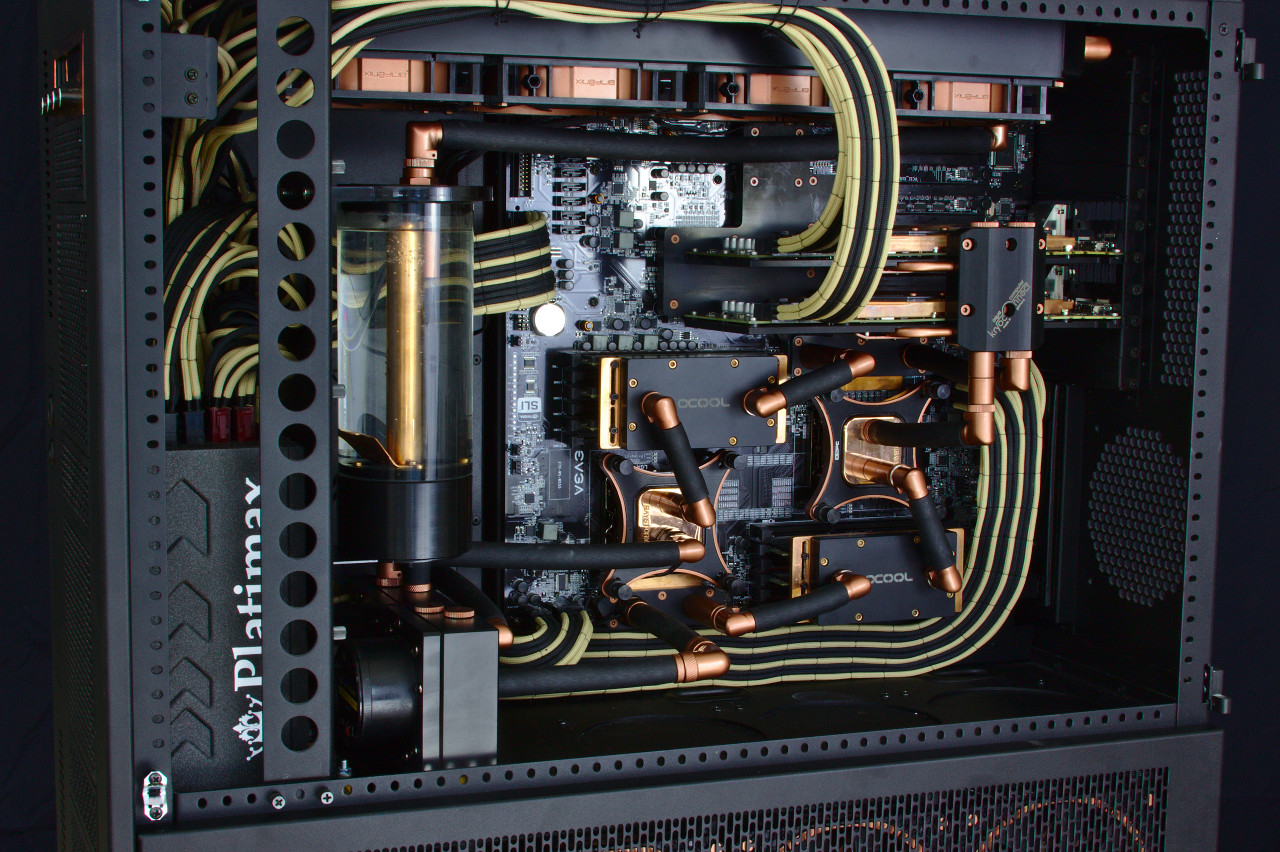
\includegraphics[width=120mm]{titlepic.jpg}

    \vfill

    \today\\
    Version 1.0.0
\end{titlingpage}
\frontmatter
\tableofcontents*

\mainmatter
\chapter{Text}
\lipsum[1]

\sffamily\lipsum[2]

\bfseries\lipsum[3]

\mdseries\ttfamily\lipsum[4]

\bfseries\ttfamily\lipsum[5]

\normalfont\scshape\lipsum[6]

\slshape\lipsum[7]

\scshape\lipsum[8]

\scslshape\lipsum[9]

\normalfont

\chapter{Tables}
\begin{table}
    \centering
    \caption{tabular inside float}
    \label{tab:float}
    \begin{tabular}{lll}
        \toprule
        \scshape Header 1 & \scshape Header 2 & \scshape Header 3 \\
        \midrule
        Content           & Content           & Content           \\
        Content           & Content           & Content           \\
        Content           & Content           & Content           \\
        Content           & Content           & Content           \\
        \bottomrule
    \end{tabular}
\end{table}

\lipsum[3]

\begin{center}
    \tabcaption{Tabular outside of float}
    \label{tab:outside}
    \begin{tabular}{lll}
        \toprule
        \scshape Header 1 & \scshape Header 2 & \scshape Header 3 \\
        \midrule
        Content           & Content           & Content           \\
        Content           & Content           & Content           \\
        Content           & Content           & Content           \\
        Content           & Content           & Content           \\
        \bottomrule
    \end{tabular}
\end{center}

\chapter{References and Hyperlinks}
This sentence refers to Table~\ref{tab:outside}.

This is a citation \cite{testitem}.

\href{https://hyperlink.com}{This is a hyperlink hiding behind text.}

\href{https://hyperlink.com}{\nolinkurl{https://hyperlink.com}}

\chapter{Sectional Headings}

This section illustrates the  style of \verb|\section|, \verb|\subsection| and
\verb|\subsubsection|.

\section{A Section}
\lipsum[2]

\subsection{A Subsection}
\lipsum[1]

\subsubsection{A subsubsection}
\lipsum[2]

\chapter{Code Listings}
\tikzset{external/export next=false}%
\begin{tcblisting}{%
        title=This Is a Code Listing,
        minted language=tex,
        listing side text,
        }
    \begin{tabular}{ll}
        a & a \\
        a & a \\
    \end{tabular}
\end{tcblisting}

\tikzset{external/export next=false}%
\begin{tcolorbox}[title=test]
    \lipsum[2]
\end{tcolorbox}

\tikzset{external/export next=false}%
\begin{tcolorbox}
    \lipsum[2]
\end{tcolorbox}

\chapter{Mathematics}

A numbered equation:
\begin{equation}
    y(x) = x^2 + 2x + 5
\end{equation}

An unnumbered equation:
\begin{equation*}
    x_{01,02} = -1 \pm 2j
\end{equation*}

An \verb|align| with some numbered and unnumbered lines:

\begin{align}
    \frac{\Phi}{i}
    & =
    \int_{0}^{\infty} \frac{dx}{x} \int_{0}^{l+m}
    \left[
        \frac{y dy}{\sqrt{x^2+y^2}} - \frac{(y-l) dy}{\sqrt{x^2+(y-l)^2}}
    \right]
    \nonumber
    \\
    &=
    \int_{0}^{\infty}
    \left[
        \sqrt{x^2 + (l+m)^2)} - \sqrt{x^2+l^2} - \sqrt{x^2+m^2}+x
    \right]
    \frac{dx}{x}
    \nonumber
    \\
    &=
    \Bigg[
        \sqrt{x^2 + (l+m)^2} - \sqrt{x^2+l^2} - \sqrt{x^2+m^2}
        \nonumber
        \\
        & ~~~~~~~~~   + x - l \cdot \log{\frac{l+m+\sqrt{x^2+(l+m)^2}}{l+\sqrt{x^2+l^2}}}
        \nonumber
        \\
        & ~~~~~~~~~   - m \cdot \log{\frac{l+m+\sqrt{x^2+(l+m)^2}}{m+\sqrt{x^2+l^2}}} ~
    \Bigg]_0^{\infty}
    \label{eq:mISL:2}
    \\
    & \approx
    \left[ l \cdot \log{\frac{l+m}{l}} + m \cdot \log{\frac{l+m}{m}} \right]
    \label{eq:mISL:3}
\end{align}


\cleardoublepage
\begin{titlingpage*}
    \fullhexpage{da2}{ct4}
    \begin{vplace}
        \flushright\Huge\bfseries\sffamily\appendixpagename
    \end{vplace}
\end{titlingpage*}
\appendix
\chapterstyle{alpenappendix}
\chapter{An Appendix Chapter}
\lipsum[1-3]

\chapter{Another Appendix Chapter with a Title That Requires Two Lines}
\lipsum[4-6]

\backmatter
\chapter{A Backmatter Chapter}
\lipsum[7-9]

\begin{thebibliography}{1}
    \bibitem{testitem}
        An Author, ``A Title``, 1979.
\end{thebibliography}
%% ============================================================== END CONTENT %
\end{document}
%</example>
% \fi
%^^A >>>
%
%^^A ------------------------------------------------------------------------- %
%^^A                                                  MULTI-LANGUAGE SUPPORT <<<
% \iffalse
%<*de>
\expandafter\newif\csname ifenglish\endcsname
\englishfalse
\input{alpenthesis.dtx}
%</de>
% \fi
%^^A >>>
%
%^^A ------------------------------------------------------------------------- %
%^^A                                                         CHARACTER TABLE <<<
% \CharacterTable
%  {Upper-case    \A\B\C\D\E\F\G\H\I\J\K\L\M\N\O\P\Q\R\S\T\U\V\W\X\Y\Z
%   Lower-case    \a\b\c\d\e\f\g\h\i\j\k\l\m\n\o\p\q\r\s\t\u\v\w\x\y\z
%   Digits        \0\1\2\3\4\5\6\7\8\9
%   Exclamation   \!     Double quote  \"     Hash (number) \#
%   Dollar        \$     Percent       \%     Ampersand     \&
%   Acute accent  \'     Left paren    \(     Right paren   \)
%   Asterisk      \*     Plus          \+     Comma         \,
%   Minus         \-     Point         \.     Solidus       \/
%   Colon         \:     Semicolon     \;     Less than     \<
%   Equals        \=     Greater than  \>     Question mark \?
%   Commercial at \@     Left bracket  \[     Backslash     \\
%   Right bracket \]     Circumflex    \^     Underscore    \_
%   Grave accent  \`     Left brace    \{     Vertical bar  \|
%   Right brace   \}     Tilde         \~}
%^^A >>>
\endinput
%^^A vim: foldenable foldcolumn=4 foldmethod=marker foldmarker=<<<,>>>

%</de>
% \fi
%^^A >>>
%
%^^A ------------------------------------------------------------------------- %
%^^A                                                         CHARACTER TABLE <<<
% \CharacterTable
%  {Upper-case    \A\B\C\D\E\F\G\H\I\J\K\L\M\N\O\P\Q\R\S\T\U\V\W\X\Y\Z
%   Lower-case    \a\b\c\d\e\f\g\h\i\j\k\l\m\n\o\p\q\r\s\t\u\v\w\x\y\z
%   Digits        \0\1\2\3\4\5\6\7\8\9
%   Exclamation   \!     Double quote  \"     Hash (number) \#
%   Dollar        \$     Percent       \%     Ampersand     \&
%   Acute accent  \'     Left paren    \(     Right paren   \)
%   Asterisk      \*     Plus          \+     Comma         \,
%   Minus         \-     Point         \.     Solidus       \/
%   Colon         \:     Semicolon     \;     Less than     \<
%   Equals        \=     Greater than  \>     Question mark \?
%   Commercial at \@     Left bracket  \[     Backslash     \\
%   Right bracket \]     Circumflex    \^     Underscore    \_
%   Grave accent  \`     Left brace    \{     Vertical bar  \|
%   Right brace   \}     Tilde         \~}
%^^A >>>
\endinput
%^^A vim: foldenable foldcolumn=4 foldmethod=marker foldmarker=<<<,>>>

%</de>
% \fi
%^^A >>>
%
%^^A ------------------------------------------------------------------------- %
%^^A                                                         CHARACTER TABLE <<<
% \CharacterTable
%  {Upper-case    \A\B\C\D\E\F\G\H\I\J\K\L\M\N\O\P\Q\R\S\T\U\V\W\X\Y\Z
%   Lower-case    \a\b\c\d\e\f\g\h\i\j\k\l\m\n\o\p\q\r\s\t\u\v\w\x\y\z
%   Digits        \0\1\2\3\4\5\6\7\8\9
%   Exclamation   \!     Double quote  \"     Hash (number) \#
%   Dollar        \$     Percent       \%     Ampersand     \&
%   Acute accent  \'     Left paren    \(     Right paren   \)
%   Asterisk      \*     Plus          \+     Comma         \,
%   Minus         \-     Point         \.     Solidus       \/
%   Colon         \:     Semicolon     \;     Less than     \<
%   Equals        \=     Greater than  \>     Question mark \?
%   Commercial at \@     Left bracket  \[     Backslash     \\
%   Right bracket \]     Circumflex    \^     Underscore    \_
%   Grave accent  \`     Left brace    \{     Vertical bar  \|
%   Right brace   \}     Tilde         \~}
%^^A >>>
\endinput
%^^A vim: foldenable foldcolumn=4 foldmethod=marker foldmarker=<<<,>>>

%</de>
% \fi
%^^A >>>
%
%^^A ------------------------------------------------------------------------- %
%^^A                                                         CHARACTER TABLE <<<
% \CharacterTable
%  {Upper-case    \A\B\C\D\E\F\G\H\I\J\K\L\M\N\O\P\Q\R\S\T\U\V\W\X\Y\Z
%   Lower-case    \a\b\c\d\e\f\g\h\i\j\k\l\m\n\o\p\q\r\s\t\u\v\w\x\y\z
%   Digits        \0\1\2\3\4\5\6\7\8\9
%   Exclamation   \!     Double quote  \"     Hash (number) \#
%   Dollar        \$     Percent       \%     Ampersand     \&
%   Acute accent  \'     Left paren    \(     Right paren   \)
%   Asterisk      \*     Plus          \+     Comma         \,
%   Minus         \-     Point         \.     Solidus       \/
%   Colon         \:     Semicolon     \;     Less than     \<
%   Equals        \=     Greater than  \>     Question mark \?
%   Commercial at \@     Left bracket  \[     Backslash     \\
%   Right bracket \]     Circumflex    \^     Underscore    \_
%   Grave accent  \`     Left brace    \{     Vertical bar  \|
%   Right brace   \}     Tilde         \~}
%^^A >>>
\endinput
%^^A vim: foldenable foldcolumn=4 foldmethod=marker foldmarker=<<<,>>>
